\documentclass[twoside]{book}

% Packages required by doxygen
\usepackage{calc}
\usepackage{doxygen}
\usepackage{graphicx}
\usepackage[utf8]{inputenc}
\usepackage{makeidx}
\usepackage{multicol}
\usepackage{multirow}
\usepackage{textcomp}
\usepackage[table]{xcolor}

% Font selection
\usepackage[T1]{fontenc}
\usepackage{mathptmx}
\usepackage[scaled=.90]{helvet}
\usepackage{courier}
\usepackage{amssymb}
\usepackage{sectsty}
\renewcommand{\familydefault}{\sfdefault}
\allsectionsfont{%
  \fontseries{bc}\selectfont%
  \color{darkgray}%
}
\renewcommand{\DoxyLabelFont}{%
  \fontseries{bc}\selectfont%
  \color{darkgray}%
}

% Page & text layout
\usepackage{geometry}
\geometry{%
  a4paper,%
  top=2.5cm,%
  bottom=2.5cm,%
  left=2.5cm,%
  right=2.5cm%
}
\tolerance=750
\hfuzz=15pt
\hbadness=750
\setlength{\emergencystretch}{15pt}
\setlength{\parindent}{0cm}
\setlength{\parskip}{0.2cm}
\makeatletter
\renewcommand{\paragraph}{%
  \@startsection{paragraph}{4}{0ex}{-1.0ex}{1.0ex}{%
    \normalfont\normalsize\bfseries\SS@parafont%
  }%
}
\renewcommand{\subparagraph}{%
  \@startsection{subparagraph}{5}{0ex}{-1.0ex}{1.0ex}{%
    \normalfont\normalsize\bfseries\SS@subparafont%
  }%
}
\makeatother

% Headers & footers
\usepackage{fancyhdr}
\pagestyle{fancyplain}
\fancyhead[LE]{\fancyplain{}{\bfseries\thepage}}
\fancyhead[CE]{\fancyplain{}{}}
\fancyhead[RE]{\fancyplain{}{\bfseries\leftmark}}
\fancyhead[LO]{\fancyplain{}{\bfseries\rightmark}}
\fancyhead[CO]{\fancyplain{}{}}
\fancyhead[RO]{\fancyplain{}{\bfseries\thepage}}
\fancyfoot[LE]{\fancyplain{}{}}
\fancyfoot[CE]{\fancyplain{}{}}
\fancyfoot[RE]{\fancyplain{}{\bfseries\scriptsize Generated on Mon Feb 2 2015 08\-:44\-:14 for N\-A\-Triu\-M by Doxygen }}
\fancyfoot[LO]{\fancyplain{}{\bfseries\scriptsize Generated on Mon Feb 2 2015 08\-:44\-:14 for N\-A\-Triu\-M by Doxygen }}
\fancyfoot[CO]{\fancyplain{}{}}
\fancyfoot[RO]{\fancyplain{}{}}
\renewcommand{\footrulewidth}{0.4pt}
\renewcommand{\chaptermark}[1]{%
  \markboth{#1}{}%
}
\renewcommand{\sectionmark}[1]{%
  \markright{\thesection\ #1}%
}

% Indices & bibliography
\usepackage{natbib}
\usepackage[titles]{tocloft}
\setcounter{tocdepth}{3}
\setcounter{secnumdepth}{5}
\makeindex

% Hyperlinks (required, but should be loaded last)
\usepackage{ifpdf}
\ifpdf
  \usepackage[pdftex,pagebackref=true]{hyperref}
\else
  \usepackage[ps2pdf,pagebackref=true]{hyperref}
\fi
\hypersetup{%
  colorlinks=true,%
  linkcolor=blue,%
  citecolor=blue,%
  unicode%
}

% Custom commands
\newcommand{\clearemptydoublepage}{%
  \newpage{\pagestyle{empty}\cleardoublepage}%
}


%===== C O N T E N T S =====

\begin{document}

% Titlepage & ToC
\hypersetup{pageanchor=false}
\pagenumbering{roman}
\begin{titlepage}
\vspace*{7cm}
\begin{center}%
{\Large N\-A\-Triu\-M }\\
\vspace*{1cm}
{\large Generated by Doxygen 1.8.6}\\
\vspace*{0.5cm}
{\small Mon Feb 2 2015 08:44:14}\\
\end{center}
\end{titlepage}
\clearemptydoublepage
\tableofcontents
\clearemptydoublepage
\pagenumbering{arabic}
\hypersetup{pageanchor=true}

%--- Begin generated contents ---
\chapter{N\-A\-Triu\-M -\/ A discontinuous Galerkin Lattice Boltzmann simulation tool based on deal.\-I\-I}
\label{index}\hypertarget{index}{}\hypertarget{index_lbm_sec}{}\section{The Lattice Boltzmann Method}\label{index_lbm_sec}
Lattice Boltzmann (LB) methods are an alternative approach for the simulation of fluid flows. Modeling particulate processes (advection and collision) they indirectly solve the fluid mechanical Navier-\/Stokes equations. Since 1988 LB has established besides classical finite element, finite volume and finite difference schemes, particularly for the simulation of complex flows. Concretely, they provide a straightforwardmodeling of multiphase flows and flows in complex geometries. Both kinds of simulations are nowadays indispensable, especially in engineering applications. The LB method has proven suitable for simulating complex flows on parallel computers. However, the original LB algorithm is limited to regular computation grids (the lattices), which is a severe shortcoming, specifically in resolving different scales and flows at high Reynolds numbers (Re). Furthermore, it is restricted to at most second order accuracy in time and space due to the inherent Euler time integration. Consequently, researchers attempted to transfer the LB concept to irregular grids and higher order accuracy. Various approaches have been published.\hypertarget{index_sedg_sec}{}\section{LBM on unstructured grids}\label{index_sedg_sec}
A very promising approach for LBM on irregular grids was published by Lee and Lin in 2003. They managed to split the Boltzmann equation into collision and advection, without restricting it to regular grids. They could solve the advection equation (streaming step) using a Finite Element scheme on a triangular grid with high order and even implicit time integrators. Their method was picked up by Min and Lee in 2011, who used a spectral element discontinuous Galerkin (SEDG) solver for the advection and obtained a high-\/order convergent SEDG-\/LBM scheme. NATriuM is based on this approach. Obviously, the sophisticated streaming procedure comes at the price of higher computation time. We have measured factors of $\sim$60 in a comparison with the Open Source LBM software Palabos (for BGK-\/collision and equal CFL numbers).\hypertarget{index_tpl_sec}{}\section{Third party libraries (TPLs)}\label{index_tpl_sec}
NATriuM inherits a huge part of its functionality from third party libraries, most importantly deal.II. Deal.II is a finite element library which was awarded the Wilkinson price for numerical software in 2007. Together with a huge FEM functionality, it offers wrappers to other TPLs like Trilinos to speed up simulations on multicore architectures. We use the Trilinos data structures (sparse matrices and vectors). The boost unit test module is used to structure the testing code. CMake is used for user-\/friendly compilation.\hypertarget{index_struct_sec}{}\section{Code structure}\label{index_struct_sec}
At the moment, NATriuM can only be used as a library, but it is going to be usable from the command line in a later stage of the project. A class diagram is in the documentation folder, but it could be slightly outdated. The source directory contains the following folders:
\begin{DoxyItemize}
\item \hyperlink{namespacenatrium}{natrium}: NATriuM library. Contains the code for the SEDG-\/Solver.
\item test: Unit and integration tests.
\item doc: Code documentation. Most importantly, this Doxygen documentation.
\item examples: Example simulations that use the NATriuM code.
\item analysis: Scripts for numerical analysis of the code (convergence tests, etc.)
\item preprocessing: Parameter GUI.
\item postprocessing: Nothing special (at the moment).
\end{DoxyItemize}\hypertarget{index_workflow_sec}{}\section{Workflow}\label{index_workflow_sec}
It is recommended to use the code in connection with sophisticated pre-\/ and postprocessing tools.
\begin{DoxyItemize}
\item Preprocessing: Deal.II supports various mesh grid formats. E.g. Salome can be used for grid generation.
\item Postprocessing: Paraview is highly recommended.
\end{DoxyItemize}

The Open Fuel Cell simulator (OpenFCST) also uses the workflow Salome-\/$>$deal.II-\/$>$Paraview. It might be interesting for you to take a look at the OpenFCST user manual (online available) which includes for example a short Tutorial on interfacing Salome and deal.II.\hypertarget{index_start_sec}{}\section{Getting started}\label{index_start_sec}
For simple applications, the triangulation can be generated within deal.II. The examples in the Examples section will help you to get grip on the code.\hypertarget{index_install_sec}{}\section{Installation}\label{index_install_sec}
The installation of NATRiuM requires several third party libraries. For a detailed documentation see the file INSTALL.txt. 
\chapter{Namespace Index}
\section{Namespace List}
Here is a list of all documented namespaces with brief descriptions:\begin{DoxyCompactList}
\item\contentsline{section}{\hyperlink{namespacenatrium}{natrium} (Definition of Grad's function to reconstruct missing distribution functions, e.g. at boundaries )}{\pageref{namespacenatrium}}{}
\item\contentsline{section}{\hyperlink{namespacenatrium_1_1CFDSolverUtilities}{natrium::CFDSolverUtilities} (Some tools for the \hyperlink{classnatrium_1_1CFDSolver}{CFDSolver} and its simple usage )}{\pageref{namespacenatrium_1_1CFDSolverUtilities}}{}
\item\contentsline{section}{\hyperlink{namespacenatrium_1_1DealIIExtensions}{natrium::DealIIExtensions} (Some extensions to deal.ii )}{\pageref{namespacenatrium_1_1DealIIExtensions}}{}
\item\contentsline{section}{\hyperlink{namespacenatrium_1_1Math}{natrium::Math} (Namespace which contains basic math functions )}{\pageref{namespacenatrium_1_1Math}}{}
\end{DoxyCompactList}

\chapter{Hierarchical Index}
\section{Class Hierarchy}
This inheritance list is sorted roughly, but not completely, alphabetically:\begin{DoxyCompactList}
\item \contentsline{section}{natrium::AdvectionOperator$<$ dim $>$}{\pageref{classnatrium_1_1AdvectionOperator}}{}
\begin{DoxyCompactList}
\item \contentsline{section}{natrium::SEDGMinLee$<$ dim $>$}{\pageref{classnatrium_1_1SEDGMinLee}}{}
\end{DoxyCompactList}
\item \contentsline{section}{natrium::AdvectionBenchmark::AdvectionResult}{\pageref{structnatrium_1_1AdvectionBenchmark_1_1AdvectionResult}}{}
\item \contentsline{section}{natrium::TaylorGreenVortex2D::AnalyticDensity}{\pageref{classnatrium_1_1TaylorGreenVortex2D_1_1AnalyticDensity}}{}
\item \contentsline{section}{natrium::CouetteFlow3D::AnalyticVelocity}{\pageref{classnatrium_1_1CouetteFlow3D_1_1AnalyticVelocity}}{}
\item \contentsline{section}{natrium::TaylorGreenVortex3D::AnalyticVelocity}{\pageref{classnatrium_1_1TaylorGreenVortex3D_1_1AnalyticVelocity}}{}
\item \contentsline{section}{natrium::PoiseuilleFlow2D::AnalyticVelocity}{\pageref{classnatrium_1_1PoiseuilleFlow2D_1_1AnalyticVelocity}}{}
\item \contentsline{section}{natrium::CouetteFlow2D::AnalyticVelocity}{\pageref{classnatrium_1_1CouetteFlow2D_1_1AnalyticVelocity}}{}
\item \contentsline{section}{natrium::TaylorGreenVortex2D::AnalyticVelocity}{\pageref{classnatrium_1_1TaylorGreenVortex2D_1_1AnalyticVelocity}}{}
\item \contentsline{section}{natrium::BGKTransformedWithConstantForce}{\pageref{classnatrium_1_1BGKTransformedWithConstantForce}}{}
\item \contentsline{section}{natrium::Boundary$<$ dim $>$}{\pageref{classnatrium_1_1Boundary}}{}
\begin{DoxyCompactList}
\item \contentsline{section}{natrium::MinLeeBoundary$<$ dim $>$}{\pageref{classnatrium_1_1MinLeeBoundary}}{}
\item \contentsline{section}{natrium::PeriodicBoundary$<$ dim $>$}{\pageref{classnatrium_1_1PeriodicBoundary}}{}
\end{DoxyCompactList}
\item \contentsline{section}{natrium::BoundaryCollection$<$ dim $>$}{\pageref{classnatrium_1_1BoundaryCollection}}{}
\item \contentsline{section}{natrium::BoundaryDensity$<$ dim $>$}{\pageref{classnatrium_1_1BoundaryDensity}}{}
\item \contentsline{section}{natrium::BoundaryTestDensity}{\pageref{classnatrium_1_1BoundaryTestDensity}}{}
\item \contentsline{section}{natrium::BoundaryTestVelocity}{\pageref{classnatrium_1_1BoundaryTestVelocity}}{}
\item \contentsline{section}{natrium::BoundaryVelocity$<$ dim $>$}{\pageref{classnatrium_1_1BoundaryVelocity}}{}
\item \contentsline{section}{natrium::CFDSolver$<$ dim $>$}{\pageref{classnatrium_1_1CFDSolver}}{}
\begin{DoxyCompactList}
\item \contentsline{section}{natrium::BenchmarkCFDSolver$<$ dim $>$}{\pageref{classnatrium_1_1BenchmarkCFDSolver}}{}
\end{DoxyCompactList}
\item \contentsline{section}{natrium::CollisionModel}{\pageref{classnatrium_1_1CollisionModel}}{}
\begin{DoxyCompactList}
\item \contentsline{section}{natrium::BGK}{\pageref{classnatrium_1_1BGK}}{}
\begin{DoxyCompactList}
\item \contentsline{section}{natrium::BGKPseudopotential}{\pageref{classnatrium_1_1BGKPseudopotential}}{}
\item \contentsline{section}{natrium::BGKStandard}{\pageref{classnatrium_1_1BGKStandard}}{}
\item \contentsline{section}{natrium::BGKStandardTransformed}{\pageref{classnatrium_1_1BGKStandardTransformed}}{}
\item \contentsline{section}{natrium::BGKSteadyState}{\pageref{classnatrium_1_1BGKSteadyState}}{}
\end{DoxyCompactList}
\end{DoxyCompactList}
\item \contentsline{section}{natrium::DistributionFunctions}{\pageref{classnatrium_1_1DistributionFunctions}}{}
\item \contentsline{section}{natrium::ErrorStats$<$ dim $>$}{\pageref{classnatrium_1_1ErrorStats}}{}
\item \contentsline{section}{HtmlTrace}{\pageref{classHtmlTrace}}{}
\item \contentsline{section}{natrium::LubricationSine::InitialVelocity}{\pageref{classnatrium_1_1LubricationSine_1_1InitialVelocity}}{}
\item \contentsline{section}{natrium::SteadyPeriodicTestFlow2D::InitialVelocity}{\pageref{classnatrium_1_1SteadyPeriodicTestFlow2D_1_1InitialVelocity}}{}
\item \contentsline{section}{natrium::SinusoidalShear2D::InitialVelocity}{\pageref{classnatrium_1_1SinusoidalShear2D_1_1InitialVelocity}}{}
\item \contentsline{section}{natrium::InitMPI}{\pageref{structnatrium_1_1InitMPI}}{}
\item \contentsline{section}{natrium::Logging}{\pageref{classnatrium_1_1Logging}}{}
\item \contentsline{section}{natrium::matrixAnalysis$<$ dim $>$}{\pageref{classnatrium_1_1matrixAnalysis}}{}
\item \contentsline{section}{plb::ModIncomprFlowParam$<$ T $>$}{\pageref{classplb_1_1ModIncomprFlowParam}}{}
\item \contentsline{section}{natrium::MPIGuard}{\pageref{classnatrium_1_1MPIGuard}}{}
\item \contentsline{section}{natrium::NATriuMException}{\pageref{classnatrium_1_1NATriuMException}}{}
\begin{DoxyCompactList}
\item \contentsline{section}{natrium::AdvectionSolverException}{\pageref{classnatrium_1_1AdvectionSolverException}}{}
\item \contentsline{section}{natrium::BoundaryCollectionException}{\pageref{classnatrium_1_1BoundaryCollectionException}}{}
\item \contentsline{section}{natrium::CFDSolverException}{\pageref{classnatrium_1_1CFDSolverException}}{}
\item \contentsline{section}{natrium::CFDSolverUtilities::CFDSolverUtilitiesException}{\pageref{classnatrium_1_1CFDSolverUtilities_1_1CFDSolverUtilitiesException}}{}
\item \contentsline{section}{natrium::CollisionException}{\pageref{classnatrium_1_1CollisionException}}{}
\item \contentsline{section}{natrium::ConfigurationException}{\pageref{classnatrium_1_1ConfigurationException}}{}
\item \contentsline{section}{natrium::PeriodicBoundaryNotPossible}{\pageref{classnatrium_1_1PeriodicBoundaryNotPossible}}{}
\end{DoxyCompactList}
\item \contentsline{section}{natrium::own\_\-double\_\-less}{\pageref{classnatrium_1_1own__double__less}}{}
\item \contentsline{section}{natrium::PhysicalProperties$<$ dim $>$}{\pageref{classnatrium_1_1PhysicalProperties}}{}
\item \contentsline{section}{natrium::BoundaryTools::point\_\-sorter}{\pageref{classnatrium_1_1BoundaryTools_1_1point__sorter}}{}
\item \contentsline{section}{natrium::ProblemDescription$<$ dim $>$}{\pageref{classnatrium_1_1ProblemDescription}}{}
\begin{DoxyCompactList}
\item \contentsline{section}{natrium::Benchmark$<$ 2 $>$}{\pageref{classnatrium_1_1Benchmark}}{}
\begin{DoxyCompactList}
\item \contentsline{section}{natrium::CouetteFlow2D}{\pageref{classnatrium_1_1CouetteFlow2D}}{}
\item \contentsline{section}{natrium::PoiseuilleFlow2D}{\pageref{classnatrium_1_1PoiseuilleFlow2D}}{}
\item \contentsline{section}{natrium::TaylorGreenVortex2D}{\pageref{classnatrium_1_1TaylorGreenVortex2D}}{}
\end{DoxyCompactList}
\item \contentsline{section}{natrium::Benchmark$<$ 3 $>$}{\pageref{classnatrium_1_1Benchmark}}{}
\begin{DoxyCompactList}
\item \contentsline{section}{natrium::CouetteFlow3D}{\pageref{classnatrium_1_1CouetteFlow3D}}{}
\item \contentsline{section}{natrium::TaylorGreenVortex3D}{\pageref{classnatrium_1_1TaylorGreenVortex3D}}{}
\end{DoxyCompactList}
\item \contentsline{section}{natrium::Benchmark$<$ dim $>$}{\pageref{classnatrium_1_1Benchmark}}{}
\end{DoxyCompactList}
\item \contentsline{section}{natrium::ProblemDescription$<$ 2 $>$}{\pageref{classnatrium_1_1ProblemDescription}}{}
\begin{DoxyCompactList}
\item \contentsline{section}{natrium::ComplexWall1}{\pageref{classnatrium_1_1ComplexWall1}}{}
\item \contentsline{section}{natrium::Cylinder2D}{\pageref{classnatrium_1_1Cylinder2D}}{}
\item \contentsline{section}{natrium::DensityFluctuation2D}{\pageref{classnatrium_1_1DensityFluctuation2D}}{}
\item \contentsline{section}{natrium::LidDrivenCavity2D}{\pageref{classnatrium_1_1LidDrivenCavity2D}}{}
\item \contentsline{section}{natrium::LubricationSine}{\pageref{classnatrium_1_1LubricationSine}}{}
\item \contentsline{section}{natrium::PeriodicTestDomain2D}{\pageref{classnatrium_1_1PeriodicTestDomain2D}}{}
\item \contentsline{section}{natrium::SinusoidalShear2D}{\pageref{classnatrium_1_1SinusoidalShear2D}}{}
\item \contentsline{section}{natrium::SteadyPeriodicTestFlow2D}{\pageref{classnatrium_1_1SteadyPeriodicTestFlow2D}}{}
\begin{DoxyCompactList}
\item \contentsline{section}{natrium::UnsteadyPeriodicTestFlow2D}{\pageref{classnatrium_1_1UnsteadyPeriodicTestFlow2D}}{}
\end{DoxyCompactList}
\item \contentsline{section}{TaylorGreenTest2D}{\pageref{classTaylorGreenTest2D}}{}
\item \contentsline{section}{WallTestDomain2D}{\pageref{classWallTestDomain2D}}{}
\end{DoxyCompactList}
\item \contentsline{section}{natrium::ProblemDescription$<$ 3 $>$}{\pageref{classnatrium_1_1ProblemDescription}}{}
\begin{DoxyCompactList}
\item \contentsline{section}{natrium::PeriodicTestDomain3D}{\pageref{classnatrium_1_1PeriodicTestDomain3D}}{}
\end{DoxyCompactList}
\item \contentsline{section}{natrium::SemiParallelMatrix$<$ VECTOR $>$}{\pageref{classnatrium_1_1SemiParallelMatrix}}{}
\item \contentsline{section}{SinusShapeDomain2D$<$ T $>$}{\pageref{classSinusShapeDomain2D}}{}
\item \contentsline{section}{natrium::SolverConfiguration}{\pageref{classnatrium_1_1SolverConfiguration}}{}
\item \contentsline{section}{natrium::SolverStats$<$ dim $>$}{\pageref{classnatrium_1_1SolverStats}}{}
\item \contentsline{section}{natrium::Stencil}{\pageref{classnatrium_1_1Stencil}}{}
\begin{DoxyCompactList}
\item \contentsline{section}{natrium::D2Q9}{\pageref{classnatrium_1_1D2Q9}}{}
\item \contentsline{section}{natrium::D3Q19}{\pageref{classnatrium_1_1D3Q19}}{}
\end{DoxyCompactList}
\item \contentsline{section}{natrium::IntegrationTestCases::TestResult}{\pageref{structnatrium_1_1IntegrationTestCases_1_1TestResult}}{}
\item \contentsline{section}{natrium::TimeIntegrator$<$ MATRIX, VECTOR $>$}{\pageref{classnatrium_1_1TimeIntegrator}}{}
\begin{DoxyCompactList}
\item \contentsline{section}{natrium::DealIIWrapper$<$ MATRIX, VECTOR $>$}{\pageref{classnatrium_1_1DealIIWrapper}}{}
\item \contentsline{section}{natrium::ExponentialTimeIntegrator$<$ MATRIX, VECTOR $>$}{\pageref{classnatrium_1_1ExponentialTimeIntegrator}}{}
\item \contentsline{section}{natrium::RungeKutta5LowStorage$<$ MATRIX, VECTOR $>$}{\pageref{classnatrium_1_1RungeKutta5LowStorage}}{}
\item \contentsline{section}{natrium::ThetaMethod$<$ MATRIX, VECTOR $>$}{\pageref{classnatrium_1_1ThetaMethod}}{}
\end{DoxyCompactList}
\item \contentsline{section}{natrium::UnsteadyPeriodicTestFlow2D::UnsteadyInitialVelocity}{\pageref{classnatrium_1_1UnsteadyPeriodicTestFlow2D_1_1UnsteadyInitialVelocity}}{}
\end{DoxyCompactList}

\chapter{Class Index}
\section{Class List}
Here are the classes, structs, unions and interfaces with brief descriptions\-:\begin{DoxyCompactList}
\item\contentsline{section}{\hyperlink{classnatrium_1_1AdvectionOperator}{natrium\-::\-Advection\-Operator$<$ dim $>$} \\*Abstract class for spatial part of the Advection Operator e\-\_\-i $\ast$ dx\-\_\-i f }{\pageref{classnatrium_1_1AdvectionOperator}}{}
\item\contentsline{section}{\hyperlink{classnatrium_1_1AdvectionSolverException}{natrium\-::\-Advection\-Solver\-Exception} \\*Exception class for Advection\-Solver }{\pageref{classnatrium_1_1AdvectionSolverException}}{}
\item\contentsline{section}{\hyperlink{classnatrium_1_1Benchmark}{natrium\-::\-Benchmark$<$ dim $>$} }{\pageref{classnatrium_1_1Benchmark}}{}
\item\contentsline{section}{\hyperlink{classnatrium_1_1BenchmarkCFDSolver}{natrium\-::\-Benchmark\-C\-F\-D\-Solver$<$ dim $>$} \\*Class that overrides the output function of the C\-F\-D solver class with comparisons to a reference solution }{\pageref{classnatrium_1_1BenchmarkCFDSolver}}{}
\item\contentsline{section}{\hyperlink{classnatrium_1_1BGKTransformed}{natrium\-::\-B\-G\-K\-Transformed} \\*Description of the B\-G\-K model for the transformed particle distributions, as described in Global data which is used by Min and Lee (2011)\-: A spectral-\/element discontinuous Galerkin lattice Boltzmann method for nearly incompressible flows, J\-C\-P 230 pp. 245-\/259 }{\pageref{classnatrium_1_1BGKTransformed}}{}
\item\contentsline{section}{\hyperlink{classnatrium_1_1BoltzmannModel}{natrium\-::\-Boltzmann\-Model} \\*Abstract class for the description of a boltzmann model, e.\-g. D2\-Q9 }{\pageref{classnatrium_1_1BoltzmannModel}}{}
\item\contentsline{section}{\hyperlink{classnatrium_1_1Boundary}{natrium\-::\-Boundary$<$ dim $>$} \\*Abstract class for the description of boundaries. Base class of \hyperlink{classnatrium_1_1PeriodicBoundary}{Periodic\-Boundary}, Inflow\-Boundary, etc }{\pageref{classnatrium_1_1Boundary}}{}
\item\contentsline{section}{\hyperlink{classnatrium_1_1BoundaryCollection}{natrium\-::\-Boundary\-Collection$<$ dim $>$} \\*The \hyperlink{classnatrium_1_1BoundaryCollection}{Boundary\-Collection} class defines all boundaries of a flow domain. Internally, the boundaries are stored in two different std\-::map, one for the periodic boundaries and one for the non-\/periodic ones. Its keys are the boundary indicators (for periodic boundaries\-: the first boundary indicator) }{\pageref{classnatrium_1_1BoundaryCollection}}{}
\item\contentsline{section}{\hyperlink{classnatrium_1_1BoundaryCollectionError}{natrium\-::\-Boundary\-Collection\-Error} \\*\hyperlink{classnatrium_1_1Boundary}{Boundary} errors (e.\-g. duplicate boundary indicators) }{\pageref{classnatrium_1_1BoundaryCollectionError}}{}
\item\contentsline{section}{\hyperlink{classnatrium_1_1BoundaryDensity}{natrium\-::\-Boundary\-Density} }{\pageref{classnatrium_1_1BoundaryDensity}}{}
\item\contentsline{section}{\hyperlink{classnatrium_1_1BoundaryTestDensity}{natrium\-::\-Boundary\-Test\-Density} }{\pageref{classnatrium_1_1BoundaryTestDensity}}{}
\item\contentsline{section}{\hyperlink{classnatrium_1_1BoundaryTestVelocity}{natrium\-::\-Boundary\-Test\-Velocity} }{\pageref{classnatrium_1_1BoundaryTestVelocity}}{}
\item\contentsline{section}{\hyperlink{classnatrium_1_1BoundaryVelocity}{natrium\-::\-Boundary\-Velocity} }{\pageref{classnatrium_1_1BoundaryVelocity}}{}
\item\contentsline{section}{\hyperlink{classnatrium_1_1CFDSolver}{natrium\-::\-C\-F\-D\-Solver$<$ dim $>$} \\*The central class for the C\-F\-D simulation based on the D\-B\-E }{\pageref{classnatrium_1_1CFDSolver}}{}
\item\contentsline{section}{\hyperlink{classnatrium_1_1CFDSolverException}{natrium\-::\-C\-F\-D\-Solver\-Exception} \\*Exception class for \hyperlink{classnatrium_1_1CFDSolver}{C\-F\-D\-Solver} }{\pageref{classnatrium_1_1CFDSolverException}}{}
\item\contentsline{section}{\hyperlink{classnatrium_1_1CollisionModel}{natrium\-::\-Collision\-Model} \\*Abstract class for the description of collision schemes }{\pageref{classnatrium_1_1CollisionModel}}{}
\item\contentsline{section}{\hyperlink{classnatrium_1_1CollisionModelException}{natrium\-::\-Collision\-Model\-Exception} \\*Exception class for Collision model }{\pageref{classnatrium_1_1CollisionModelException}}{}
\item\contentsline{section}{\hyperlink{classnatrium_1_1ConfigurationException}{natrium\-::\-Configuration\-Exception} \\*Exception class for \hyperlink{classnatrium_1_1CFDSolver}{C\-F\-D\-Solver} }{\pageref{classnatrium_1_1ConfigurationException}}{}
\item\contentsline{section}{\hyperlink{classnatrium_1_1CouetteFlow2D}{natrium\-::\-Couette\-Flow2\-D} \\*Description of a simple Couette Flow (regular channel flow in square domain). The domain is \mbox{[}0,1\mbox{]}$^\wedge$2. The top plate is moved with constant velocity. The domain consists of 8 x 8 = 64 Elements (contrast to Min and Lee, who have 6 x 6) }{\pageref{classnatrium_1_1CouetteFlow2D}}{}
\item\contentsline{section}{\hyperlink{classnatrium_1_1D2Q9IncompressibleModel}{natrium\-::\-D2\-Q9\-Incompressible\-Model} \\*D2\-Q9 model description for incompressible flow }{\pageref{classnatrium_1_1D2Q9IncompressibleModel}}{}
\item\contentsline{section}{\hyperlink{classnatrium_1_1D2Q9Model}{natrium\-::\-D2\-Q9\-Model} \\*D2\-Q9 Model }{\pageref{classnatrium_1_1D2Q9Model}}{}
\item\contentsline{section}{\hyperlink{classnatrium_1_1DistributionFunctions}{natrium\-::\-Distribution\-Functions} \\*This class contains the distribution functions. As the zero-\/velocity particles (f0) can be ignored for streaming, f0 is split from the other distribution functions (f\-Stream) in the implementation. f\-Stream is a block vector, which has the advantage that it can be multiplied with the System\-Matrix. The \hyperlink{classnatrium_1_1DistributionFunctions}{Distribution\-Functions} class is designed to mime the behaviour of a vector$<$distributed\-\_\-vector$>$ }{\pageref{classnatrium_1_1DistributionFunctions}}{}
\item\contentsline{section}{\hyperlink{classnatrium_1_1ErrorStats}{natrium\-::\-Error\-Stats$<$ dim $>$} \\*Container for error statistics and table file; only for use with \hyperlink{classnatrium_1_1BenchmarkCFDSolver}{Benchmark\-C\-F\-D\-Solver} }{\pageref{classnatrium_1_1ErrorStats}}{}
\item\contentsline{section}{\hyperlink{classnatrium_1_1ExponentialTimeIntegrator}{natrium\-::\-Exponential\-Time\-Integrator} \\*Exponential time integration scheme for the solution of f' = L$\ast$f, as used in Uga etal. (2012) Spectral-\/element discontinuous Galerkin lattice Boltzmann simulation of flow past two cylinders in tandem with an exponential time integrator, C\-M\-W\-A 65 pp. 239-\/251 }{\pageref{classnatrium_1_1ExponentialTimeIntegrator}}{}
\item\contentsline{section}{\hyperlink{classnatrium_1_1LidDrivenCavity2D}{natrium\-::\-Lid\-Driven\-Cavity2\-D} \\*Description of a simple Channel Flow The domain is \mbox{[}0,5\mbox{]}x\mbox{[}0,1\mbox{]} }{\pageref{classnatrium_1_1LidDrivenCavity2D}}{}
\item\contentsline{section}{\hyperlink{classnatrium_1_1Logging}{natrium\-::\-Logging} \\*This class is responsible for output streams to the command line and log file }{\pageref{classnatrium_1_1Logging}}{}
\item\contentsline{section}{\hyperlink{classnatrium_1_1matrixAnalysis}{natrium\-::matrix\-Analysis$<$ dim $>$} \\*Calculation of spectra and pseudospectra of streaming matrices }{\pageref{classnatrium_1_1matrixAnalysis}}{}
\item\contentsline{section}{\hyperlink{classnatrium_1_1MinLeeBoundary}{natrium\-::\-Min\-Lee\-Boundary$<$ dim $>$} \\*The boundary described by Min and Lee. For outgoing particle distribution functions the fluxes are set to 0 For incoming particle distributions fluxes are set to \[ f_{\alpha} - f^{+}_{\alpha} = f_{\alpha} - f_{\alpha^{*}} - 2w_{\alpha} \rho_{0} (e_{\alpha}\cdot u_{b})/c^{2}_{s}\] }{\pageref{classnatrium_1_1MinLeeBoundary}}{}
\item\contentsline{section}{\hyperlink{classnatrium_1_1own__double__less}{natrium\-::own\-\_\-double\-\_\-less} \\*Function to compare doubles as map keys; regards two doubles equal if they are in a epsilon(=1e-\/7)-\/range }{\pageref{classnatrium_1_1own__double__less}}{}
\item\contentsline{section}{\hyperlink{classnatrium_1_1PeriodicBoundary}{natrium\-::\-Periodic\-Boundary$<$ dim $>$} \\*A periodic boundary condition, }{\pageref{classnatrium_1_1PeriodicBoundary}}{}
\item\contentsline{section}{\hyperlink{classnatrium_1_1PeriodicBoundaryNotPossible}{natrium\-::\-Periodic\-Boundary\-Not\-Possible} \\*Exception for impossible periodic boundary, e.\-g. when the interfaces don't have the same length }{\pageref{classnatrium_1_1PeriodicBoundaryNotPossible}}{}
\item\contentsline{section}{\hyperlink{classnatrium_1_1PeriodicTestDomain2D}{natrium\-::\-Periodic\-Test\-Domain2\-D} \\*Description of a simple Periodic Flow (flow in square domain). The domain is \mbox{[}0,1\mbox{]}$^\wedge$2. The domain consists of 4 elements }{\pageref{classnatrium_1_1PeriodicTestDomain2D}}{}
\item\contentsline{section}{\hyperlink{classnatrium_1_1PhysicalProperties}{natrium\-::\-Physical\-Properties$<$ dim $>$} }{\pageref{classnatrium_1_1PhysicalProperties}}{}
\item\contentsline{section}{\hyperlink{classnatrium_1_1PoiseuilleFlow2D}{natrium\-::\-Poiseuille\-Flow2\-D} \\*Description of a simple Channel Flow The domain is \mbox{[}0,5\mbox{]}x\mbox{[}0,1\mbox{]} }{\pageref{classnatrium_1_1PoiseuilleFlow2D}}{}
\item\contentsline{section}{\hyperlink{classnatrium_1_1ProblemDescription}{natrium\-::\-Problem\-Description$<$ dim $>$} \\*Abstract class for the description of a C\-F\-D problem. The description includes the computational mesh, boundary description, viscosity and initial values }{\pageref{classnatrium_1_1ProblemDescription}}{}
\item\contentsline{section}{\hyperlink{classnatrium_1_1RungeKutta5LowStorage}{natrium\-::\-Runge\-Kutta5\-Low\-Storage$<$ M\-A\-T\-R\-I\-X, V\-E\-C\-T\-O\-R $>$} \\*Implementation of the fifth-\/order Runge-\/\-Kutta time integration scheme with low storage consumption }{\pageref{classnatrium_1_1RungeKutta5LowStorage}}{}
\item\contentsline{section}{\hyperlink{classnatrium_1_1SEDGMinLee}{natrium\-::\-S\-E\-D\-G\-Min\-Lee$<$ dim $>$} \\*This class solves the linear advection equations by a scheme which is used, e.\-g., by Min and Lee (2011)\-: A spectral-\/element discontinuous Galerkin lattice Boltzmann method for nearly incompressible flows, J\-C\-P 230 pp. 245-\/259. The advection equations used in the Lattice Boltzmann on unstructured grids are \[ \partial_t f_{\alpha} + e_{\alpha} \partial_x f_{\alpha} = 0,\quad \forall {\alpha} = 1,\dots,Q-1 \] where $ f_{\alpha}(x,t) $ are the particle distribution functions, and $ e_{\alpha} $ are the particle velocities. The discontinuous Galerkin (D\-G) method turns these P\-D\-Es into a large system of O\-D\-Es which can then be solved by a time integration scheme. Whereas this class implements the S\-E\-D\-G spatial discretization, the time integration is done by a subclass of \hyperlink{classnatrium_1_1TimeIntegrator}{Time\-Integrator}, e.\-g. \hyperlink{classnatrium_1_1RungeKutta5LowStorage}{Runge\-Kutta5\-Low\-Storage}. In other Finite Element schemes, degrees of freedom can belong to different elements (e.\-g. at corners of elements). In contrast, D\-G methods have the degrees of freedom belonging to a single element, which can lead to discontinuities at the element faces. To connect neighbor cells, the integral over the boundary of each cell incorporates the solution on neighbor cells. These contributions are called numerical fluxes. The D\-G scheme uses the weak formulation of the above equations on quadrilateral elements \$\$\-: \[ \left( \partial_t f_{\alpha} + \partial_x (e_{\alpha} f_{\alpha}), \Phi \right)_{\Omega_e} = \left(n \left[ e_i f_{\alpha} - F^{\ast}_{\alpha}(f) \right], \Phi \right)_{\partial \Omega_e}. \] In this formulation $ F^{\ast}_{i}(f) $ denotes the numerical fluxes. They can be be calculated as central fluxes or Lax-\/\-Friedrichs fluxes. Lax-\/\-Friedrichs is in general more accurate for the advection equation. For detailed information on the fluxes, see the cited paper. For spatial integration a Gauss-\/\-Lobatto quadrature is used, which has the advantage that the resulting mass matrix M\-\_\-\{\} = (, )\-\_\-\{\} is diagonal. This circumvents the solution of a linear equation system. Each advection equation leads to a O\-D\-E \[ \partial_t f_{\alpha} = M_{\alpha}^{-1}(- e_{\alpha x} D_{{\alpha}x} - e_{{\alpha}y} D_{{\alpha}y} + R_{\alpha}) f_{\alpha} + B_i f_{{\alpha}^{\ast}} + b_{\alpha}.\] Altogether, for the example of the D2\-Q9, the system becomes \[ \partial_t f_{1,\dots,Q} = \left( \matrix{ L_1 & 0 & B_1 & 0 & 0 & 0 & 0 & 0 \cr 0 & L_2 & 0 & B_2 & 0 & 0 & 0 & 0 \cr B_3 & 0 & L_3 & 0 & 0 & 0 & 0 & 0 \cr 0 & B_4 & 0 & L_4 & 0 & 0 & 0 & 0 \cr 0 & 0 & 0 & 0 & L_5 & 0 & B_5 & 0 \cr 0 & 0 & 0 & 0 & 0 & L_6 & 0 & B_6\cr 0 & 0 & 0 & 0 & B_7 & 0 & L_7 & 0 \cr 0 & 0 & 0 & 0 & 0 & B_8 & 0 & L_8 } \right) f_{1,\dots,Q} + \left( \matrix{ b_1 \cr b_2 \cr b_3 \cr b_4 \cr b_5 \cr b_6 \cr b_7 \cr b_8 }\right), \] where $ L_{\alpha} = M_{\alpha}^{-1}(- e_{{\alpha}x} D_{{\alpha}x} - e_{{\alpha}y} D_{{\alpha}y} + R_{\alpha}) $ }{\pageref{classnatrium_1_1SEDGMinLee}}{}
\item\contentsline{section}{\hyperlink{classnatrium_1_1SolverConfiguration}{natrium\-::\-Solver\-Configuration} \\*Class that stores the configuration for a C\-F\-D simulation based on the Discrete Boltzmann Equation (D\-B\-E) }{\pageref{classnatrium_1_1SolverConfiguration}}{}
\item\contentsline{section}{\hyperlink{classnatrium_1_1SolverStats}{natrium\-::\-Solver\-Stats$<$ dim $>$} \\*Container for solver statistics and table file }{\pageref{classnatrium_1_1SolverStats}}{}
\item\contentsline{section}{\hyperlink{classnatrium_1_1SteadyPeriodicTestFlow2D}{natrium\-::\-Steady\-Periodic\-Test\-Flow2\-D} \\*Description of a simple Periodic Flow (flow in square domain). The domain is \mbox{[}0,1\mbox{]}$^\wedge$2. The domain consists of 8 x 8 = 64 Elements (contrast to Min and Lee, who have 6 x 6) }{\pageref{classnatrium_1_1SteadyPeriodicTestFlow2D}}{}
\item\contentsline{section}{\hyperlink{classTaylorGreenTest2D}{Taylor\-Green\-Test2\-D} \\*Description of a Taylor-\/\-Green vortex, a benchmark with only periodic boundaries }{\pageref{classTaylorGreenTest2D}}{}
\item\contentsline{section}{\hyperlink{classnatrium_1_1TaylorGreenVortex2D}{natrium\-::\-Taylor\-Green\-Vortex2\-D} \\*Description of a simple Periodic Flow (flow in square domain). The domain is \mbox{[}0,1\mbox{]}$^\wedge$2. The domain consists of 8 x 8 = 64 Elements (contrast to Min and Lee, who have 6 x 6) }{\pageref{classnatrium_1_1TaylorGreenVortex2D}}{}
\item\contentsline{section}{\hyperlink{classnatrium_1_1TimeIntegrator}{natrium\-::\-Time\-Integrator$<$ M\-A\-T\-R\-I\-X, V\-E\-C\-T\-O\-R $>$} \\*Abstract class for time integration (solution of ordinary differential equations (O\-D\-E)) }{\pageref{classnatrium_1_1TimeIntegrator}}{}
\item\contentsline{section}{\hyperlink{classnatrium_1_1UnsteadyPeriodicTestFlow2D}{natrium\-::\-Unsteady\-Periodic\-Test\-Flow2\-D} }{\pageref{classnatrium_1_1UnsteadyPeriodicTestFlow2D}}{}
\item\contentsline{section}{\hyperlink{classWallTestDomain2D}{Wall\-Test\-Domain2\-D} \\*Description of a simple Flow with wall boundaries (flow in square domain). The domain is \mbox{[}0,1\mbox{]}$^\wedge$2. The domain consists of 4 elements }{\pageref{classWallTestDomain2D}}{}
\end{DoxyCompactList}

\chapter{File Index}
\section{File List}
Here is a list of all documented files with brief descriptions:\begin{DoxyCompactList}
\item\contentsline{section}{/mnt/fdrive/akraem3m/workspace/NATriuM/src/analysis/convergence-\/analysis-\/advection-\/solver/\hyperlink{advectionConvergence_8cpp}{advectionConvergence.cpp} (Checks the convergence of the SEDG advection solver, analyzes the local discretization error in dependence of dt, dx and fe\_\-order )}{\pageref{advectionConvergence_8cpp}}{}
\item\contentsline{section}{/mnt/fdrive/akraem3m/workspace/NATriuM/src/analysis/convergence-\/analysis-\/basic/\hyperlink{convergence-analysis-basic_8cpp}{convergence-\/analysis-\/basic.cpp} (The convergence of the NATriuM solver is analyzed by application to the Taylor-\/Green vortex in 2D (only periodic walls). This script uses a linear scaling (= constant Mach number). Thus, there is a general compressibily error, which destroys the convergence for the finer meshes. To analyze the results, move the table\_\-order.txt and table\_\-results.txt files to NATriuM/src/analysis/convergence\_\-analysis\_\-basic/ and execute the gnuplot scripts )}{\pageref{convergence-analysis-basic_8cpp}}{}
\item\contentsline{section}{/mnt/fdrive/akraem3m/workspace/NATriuM/src/analysis/convergence-\/analysis-\/junk/\hyperlink{convergence-analysis-junk_8cpp}{convergence-\/analysis-\/junk.cpp} }{\pageref{convergence-analysis-junk_8cpp}}{}
\item\contentsline{section}{/mnt/fdrive/akraem3m/workspace/NATriuM/src/analysis/convergence-\/analysis-\/kinetic-\/energy/\hyperlink{convergence-analysis-kinE_8cpp}{convergence-\/analysis-\/kinE.cpp} (Investigate the evolution of the kinetic energy over time )}{\pageref{convergence-analysis-kinE_8cpp}}{}
\item\contentsline{section}{/mnt/fdrive/akraem3m/workspace/NATriuM/src/analysis/convergence-\/analysis-\/p/\hyperlink{convergence-analysis-p_8cpp}{convergence-\/analysis-\/p.cpp} (The convergence of the NATriuM solver is analyzed by application to the Taylor-\/Green vortex in 2D (only periodic walls). This script uses a linear scaling (= constant Mach number). Thus, there is a general compressibily error, which destroys the convergence for the finer meshes. To analyze the results, move the table\_\-order.txt and table\_\-results.txt files to NATriuM/src/analysis/convergence\_\-analysis\_\-basic/ and execute the gnuplot scripts )}{\pageref{convergence-analysis-p_8cpp}}{}
\item\contentsline{section}{/mnt/fdrive/akraem3m/workspace/NATriuM/src/analysis/convergence-\/analysis/\hyperlink{convergence-analysis_8cpp}{convergence-\/analysis.cpp} (The convergence of the NATriuM solver is analyzed by application to the Taylor-\/Green vortex in 2D (only periodic walls). This script uses a linear scaling (= constant Mach number). Thus, there is a general compressibily error, which destroys the convergence for the finer meshes. To analyze the results, move the table\_\-order.txt and table\_\-results.txt files to NATriuM/src/analysis/convergence\_\-analysis\_\-basic/ and execute the gnuplot scripts )}{\pageref{convergence-analysis_8cpp}}{}
\item\contentsline{section}{/mnt/fdrive/akraem3m/workspace/NATriuM/src/analysis/matrix-\/analysis/\hyperlink{analyzeMatrix_8cpp}{analyzeMatrix.cpp} (Executable for the analysis of spectra/pseudospectra of streaming matrices )}{\pageref{analyzeMatrix_8cpp}}{}
\item\contentsline{section}{/mnt/fdrive/akraem3m/workspace/NATriuM/src/analysis/matrix-\/analysis/\hyperlink{matrixAnalysis_8cpp}{matrixAnalysis.cpp} (Computation and output of spectra/pseudospectra of streaming matrices )}{\pageref{matrixAnalysis_8cpp}}{}
\item\contentsline{section}{/mnt/fdrive/akraem3m/workspace/NATriuM/src/analysis/matrix-\/analysis/\hyperlink{matrixAnalysis_8h}{matrixAnalysis.h} (Header file for the computation of spectra/pseudospectra of streaming matrices )}{\pageref{matrixAnalysis_8h}}{}
\item\contentsline{section}{/mnt/fdrive/akraem3m/workspace/NATriuM/src/analysis/parallel\_\-benchmark/\hyperlink{benchmark_8cpp}{benchmark.cpp} (Couette Flow in 2D with time measurement )}{\pageref{benchmark_8cpp}}{}
\item\contentsline{section}{/mnt/fdrive/akraem3m/workspace/NATriuM/src/analysis/performance-\/analysis/\hyperlink{performance-analysis_8cpp}{performance-\/analysis.cpp} (The convergence of the NATriuM solver is analyzed by application to the Taylor-\/Green vortex in 2D (only periodic walls). This script uses a linear scaling (= constant Mach number). Thus, there is a general compressibily error, which destroys the convergence for the finer meshes. To analyze the results, move the table\_\-order.txt and table\_\-results.txt files to NATriuM/src/analysis/convergence\_\-analysis\_\-basic/ and execute the gnuplot scripts )}{\pageref{performance-analysis_8cpp}}{}
\item\contentsline{section}{/mnt/fdrive/akraem3m/workspace/NATriuM/src/analysis/performance-\/analysis/palabos/{\bfseries pramsmod.h} }{\pageref{pramsmod_8h}}{}
\item\contentsline{section}{/mnt/fdrive/akraem3m/workspace/NATriuM/src/examples/step-\/0/\hyperlink{LidDrivenCavity2D_8cpp}{LidDrivenCavity2D.cpp} (Lid-\/driven cavity with three static walls and one moving wall )}{\pageref{LidDrivenCavity2D_8cpp}}{}
\item\contentsline{section}{/mnt/fdrive/akraem3m/workspace/NATriuM/src/examples/step-\/0/\hyperlink{LidDrivenCavity2D_8h}{LidDrivenCavity2D.h} (Lid-\/driven cavity with three static walls and one moving wall )}{\pageref{LidDrivenCavity2D_8h}}{}
\item\contentsline{section}{/mnt/fdrive/akraem3m/workspace/NATriuM/src/examples/step-\/0/\hyperlink{step-0_8cpp}{step-\/0.cpp} }{\pageref{step-0_8cpp}}{}
\item\contentsline{section}{/mnt/fdrive/akraem3m/workspace/NATriuM/src/examples/step-\/1/\hyperlink{step-1_8cpp}{step-\/1.cpp} (Taylor-\/Green vortex in 2D (only periodic walls) )}{\pageref{step-1_8cpp}}{}
\item\contentsline{section}{/mnt/fdrive/akraem3m/workspace/NATriuM/src/examples/step-\/2/\hyperlink{step-2_8cpp}{step-\/2.cpp} (Second tutorial: Couette Flow in 2D )}{\pageref{step-2_8cpp}}{}
\item\contentsline{section}{/mnt/fdrive/akraem3m/workspace/NATriuM/src/examples/step-\/6/\hyperlink{ComplexWall1_8cpp}{ComplexWall1.cpp} }{\pageref{ComplexWall1_8cpp}}{}
\item\contentsline{section}{/mnt/fdrive/akraem3m/workspace/NATriuM/src/examples/step-\/6/{\bfseries ComplexWall1.h} }{\pageref{ComplexWall1_8h}}{}
\item\contentsline{section}{/mnt/fdrive/akraem3m/workspace/NATriuM/src/examples/step-\/9/\hyperlink{Cylinder2D_8cpp}{Cylinder2D.cpp} }{\pageref{Cylinder2D_8cpp}}{}
\item\contentsline{section}{/mnt/fdrive/akraem3m/workspace/NATriuM/src/examples/step-\/9/\hyperlink{Cylinder2D_8h}{Cylinder2D.h} (Description of the circular cylinder benchmark (Karman vortex street) )}{\pageref{Cylinder2D_8h}}{}
\item\contentsline{section}{/mnt/fdrive/akraem3m/workspace/NATriuM/src/examples/step-\/99/{\bfseries DensityFluctuation2D.h} }{\pageref{DensityFluctuation2D_8h}}{}
\item\contentsline{section}{/mnt/fdrive/akraem3m/workspace/NATriuM/src/examples/step-\/couette3D/\hyperlink{step-couette3D_8cpp}{step-\/couette3D.cpp} (Second tutorial: Couette Flow in 2D )}{\pageref{step-couette3D_8cpp}}{}
\item\contentsline{section}{/mnt/fdrive/akraem3m/workspace/NATriuM/src/examples/step-\/lubrication-\/sine/\hyperlink{step-lubrication-sine_8cpp}{step-\/lubrication-\/sine.cpp} (Sinusoidal Shear flow )}{\pageref{step-lubrication-sine_8cpp}}{}
\item\contentsline{section}{/mnt/fdrive/akraem3m/workspace/NATriuM/src/library/natrium/advection/\hyperlink{AdvectionOperator_8cpp}{AdvectionOperator.cpp} }{\pageref{AdvectionOperator_8cpp}}{}
\item\contentsline{section}{/mnt/fdrive/akraem3m/workspace/NATriuM/src/library/natrium/advection/\hyperlink{AdvectionOperator_8h}{AdvectionOperator.h} (Abstract class for spatial part of the Advection Operator e\_\-i $\ast$ dx\_\-i f )}{\pageref{AdvectionOperator_8h}}{}
\item\contentsline{section}{/mnt/fdrive/akraem3m/workspace/NATriuM/src/library/natrium/advection/\hyperlink{SEDGMinLee_8cpp}{SEDGMinLee.cpp} (Advection scheme proposed by Min and Lee (2011) )}{\pageref{SEDGMinLee_8cpp}}{}
\item\contentsline{section}{/mnt/fdrive/akraem3m/workspace/NATriuM/src/library/natrium/advection/\hyperlink{SEDGMinLee_8h}{SEDGMinLee.h} (Advection operator proposed by Min and Lee (2011): A spectral-\/elemennt discontinuous Galerkin lattice Boltzmann method for nearly incompressible flows, JCP 230 pp. 245-\/259 )}{\pageref{SEDGMinLee_8h}}{}
\item\contentsline{section}{/mnt/fdrive/akraem3m/workspace/NATriuM/src/library/natrium/benchmarks/{\bfseries AdvectionBenchmark.h} }{\pageref{AdvectionBenchmark_8h}}{}
\item\contentsline{section}{/mnt/fdrive/akraem3m/workspace/NATriuM/src/library/natrium/benchmarks/\hyperlink{CouetteFlow2D_8cpp}{CouetteFlow2D.cpp} }{\pageref{CouetteFlow2D_8cpp}}{}
\item\contentsline{section}{/mnt/fdrive/akraem3m/workspace/NATriuM/src/library/natrium/benchmarks/\hyperlink{CouetteFlow2D_8h}{CouetteFlow2D.h} (Description of a simple Couette Flow (regular channel flow in rectangular domain) )}{\pageref{CouetteFlow2D_8h}}{}
\item\contentsline{section}{/mnt/fdrive/akraem3m/workspace/NATriuM/src/library/natrium/benchmarks/\hyperlink{CouetteFlow3D_8cpp}{CouetteFlow3D.cpp} }{\pageref{CouetteFlow3D_8cpp}}{}
\item\contentsline{section}{/mnt/fdrive/akraem3m/workspace/NATriuM/src/library/natrium/benchmarks/\hyperlink{CouetteFlow3D_8h}{CouetteFlow3D.h} (Description of a simple Couette Flow (regular channel flow in rectangular domain) )}{\pageref{CouetteFlow3D_8h}}{}
\item\contentsline{section}{/mnt/fdrive/akraem3m/workspace/NATriuM/src/library/natrium/benchmarks/{\bfseries LubricationSine.h} }{\pageref{LubricationSine_8h}}{}
\item\contentsline{section}{/mnt/fdrive/akraem3m/workspace/NATriuM/src/library/natrium/benchmarks/\hyperlink{PeriodicTestDomain2D_8cpp}{PeriodicTestDomain2D.cpp} }{\pageref{PeriodicTestDomain2D_8cpp}}{}
\item\contentsline{section}{/mnt/fdrive/akraem3m/workspace/NATriuM/src/library/natrium/benchmarks/\hyperlink{PeriodicTestDomain2D_8h}{PeriodicTestDomain2D.h} (Description of a simple Periodic Flow (in rectangular domain) )}{\pageref{PeriodicTestDomain2D_8h}}{}
\item\contentsline{section}{/mnt/fdrive/akraem3m/workspace/NATriuM/src/library/natrium/benchmarks/\hyperlink{PeriodicTestDomain3D_8cpp}{PeriodicTestDomain3D.cpp} }{\pageref{PeriodicTestDomain3D_8cpp}}{}
\item\contentsline{section}{/mnt/fdrive/akraem3m/workspace/NATriuM/src/library/natrium/benchmarks/\hyperlink{PeriodicTestDomain3D_8h}{PeriodicTestDomain3D.h} (Description of a simple Periodic Flow (in rectangular domain) )}{\pageref{PeriodicTestDomain3D_8h}}{}
\item\contentsline{section}{/mnt/fdrive/akraem3m/workspace/NATriuM/src/library/natrium/benchmarks/\hyperlink{PoiseuilleFlow2D_8cpp}{PoiseuilleFlow2D.cpp} }{\pageref{PoiseuilleFlow2D_8cpp}}{}
\item\contentsline{section}{/mnt/fdrive/akraem3m/workspace/NATriuM/src/library/natrium/benchmarks/\hyperlink{PoiseuilleFlow2D_8h}{PoiseuilleFlow2D.h} (Channel flow in 2D )}{\pageref{PoiseuilleFlow2D_8h}}{}
\item\contentsline{section}{/mnt/fdrive/akraem3m/workspace/NATriuM/src/library/natrium/benchmarks/{\bfseries SinusoidalShear2D.h} }{\pageref{SinusoidalShear2D_8h}}{}
\item\contentsline{section}{/mnt/fdrive/akraem3m/workspace/NATriuM/src/library/natrium/benchmarks/\hyperlink{TaylorGreenVortex2D_8cpp}{TaylorGreenVortex2D.cpp} }{\pageref{TaylorGreenVortex2D_8cpp}}{}
\item\contentsline{section}{/mnt/fdrive/akraem3m/workspace/NATriuM/src/library/natrium/benchmarks/\hyperlink{TaylorGreenVortex2D_8h}{TaylorGreenVortex2D.h} (Description of a simple Periodic Flow (in rectangular domain) )}{\pageref{TaylorGreenVortex2D_8h}}{}
\item\contentsline{section}{/mnt/fdrive/akraem3m/workspace/NATriuM/src/library/natrium/benchmarks/\hyperlink{TaylorGreenVortex3D_8h}{TaylorGreenVortex3D.h} (Description of a simple Periodic Flow (in cubic domain) )}{\pageref{TaylorGreenVortex3D_8h}}{}
\item\contentsline{section}{/mnt/fdrive/akraem3m/workspace/NATriuM/src/library/natrium/collision/\hyperlink{BGK_8cpp}{BGK.cpp} }{\pageref{BGK_8cpp}}{}
\item\contentsline{section}{/mnt/fdrive/akraem3m/workspace/NATriuM/src/library/natrium/collision/\hyperlink{BGK_8h}{BGK.h} (Description of the BGK model for the transformed particle distributions, as described in Global data which is used by Min and Lee (2011): A spectral-\/element discontinuous Galerkin lattice Boltzmann method for nearly incompressible flows, JCP 230 pp. 245-\/259 )}{\pageref{BGK_8h}}{}
\item\contentsline{section}{/mnt/fdrive/akraem3m/workspace/NATriuM/src/library/natrium/collision/{\bfseries BGKPseudopotential.h} }{\pageref{BGKPseudopotential_8h}}{}
\item\contentsline{section}{/mnt/fdrive/akraem3m/workspace/NATriuM/src/library/natrium/collision/\hyperlink{BGKStandard_8cpp}{BGKStandard.cpp} (D2Q9 model description for incompressible flow )}{\pageref{BGKStandard_8cpp}}{}
\item\contentsline{section}{/mnt/fdrive/akraem3m/workspace/NATriuM/src/library/natrium/collision/\hyperlink{BGKStandard_8h}{BGKStandard.h} (D2Q9 model description for incompressible flow )}{\pageref{BGKStandard_8h}}{}
\item\contentsline{section}{/mnt/fdrive/akraem3m/workspace/NATriuM/src/library/natrium/collision/\hyperlink{BGKStandardTransformed_8cpp}{BGKStandardTransformed.cpp} (D2Q9 model description for incompressible flow )}{\pageref{BGKStandardTransformed_8cpp}}{}
\item\contentsline{section}{/mnt/fdrive/akraem3m/workspace/NATriuM/src/library/natrium/collision/\hyperlink{BGKStandardTransformed_8h}{BGKStandardTransformed.h} (D2Q9 model description for incompressible flow )}{\pageref{BGKStandardTransformed_8h}}{}
\item\contentsline{section}{/mnt/fdrive/akraem3m/workspace/NATriuM/src/library/natrium/collision/\hyperlink{BGKSteadyState_8cpp}{BGKSteadyState.cpp} (D2Q9 model description for incompressible flow )}{\pageref{BGKSteadyState_8cpp}}{}
\item\contentsline{section}{/mnt/fdrive/akraem3m/workspace/NATriuM/src/library/natrium/collision/\hyperlink{BGKSteadyState_8h}{BGKSteadyState.h} (D2Q9 model description for incompressible flow )}{\pageref{BGKSteadyState_8h}}{}
\item\contentsline{section}{/mnt/fdrive/akraem3m/workspace/NATriuM/src/library/natrium/collision/\hyperlink{CollisionModel_8cpp}{CollisionModel.cpp} }{\pageref{CollisionModel_8cpp}}{}
\item\contentsline{section}{/mnt/fdrive/akraem3m/workspace/NATriuM/src/library/natrium/collision/\hyperlink{CollisionModel_8h}{CollisionModel.h} (Abstract class for the description of collision schemes )}{\pageref{CollisionModel_8h}}{}
\item\contentsline{section}{/mnt/fdrive/akraem3m/workspace/NATriuM/src/library/natrium/problemdescription/\hyperlink{Benchmark_8cpp}{Benchmark.cpp} (Abstract class for the description of a CFD Benchmark problem )}{\pageref{Benchmark_8cpp}}{}
\item\contentsline{section}{/mnt/fdrive/akraem3m/workspace/NATriuM/src/library/natrium/problemdescription/\hyperlink{Benchmark_8h}{Benchmark.h} (Abstract class for the description of a CFD Benchmark problem )}{\pageref{Benchmark_8h}}{}
\item\contentsline{section}{/mnt/fdrive/akraem3m/workspace/NATriuM/src/library/natrium/problemdescription/\hyperlink{Boundary_8cpp}{Boundary.cpp} (Abstract class for the description of boundary conditions )}{\pageref{Boundary_8cpp}}{}
\item\contentsline{section}{/mnt/fdrive/akraem3m/workspace/NATriuM/src/library/natrium/problemdescription/\hyperlink{Boundary_8h}{Boundary.h} (Abstract class for Description of a Boundary object )}{\pageref{Boundary_8h}}{}
\item\contentsline{section}{/mnt/fdrive/akraem3m/workspace/NATriuM/src/library/natrium/problemdescription/{\bfseries BoundaryCollection.h} }{\pageref{BoundaryCollection_8h}}{}
\item\contentsline{section}{/mnt/fdrive/akraem3m/workspace/NATriuM/src/library/natrium/problemdescription/\hyperlink{BoundaryTools_8cpp}{BoundaryTools.cpp} }{\pageref{BoundaryTools_8cpp}}{}
\item\contentsline{section}{/mnt/fdrive/akraem3m/workspace/NATriuM/src/library/natrium/problemdescription/\hyperlink{BoundaryTools_8h}{BoundaryTools.h} }{\pageref{BoundaryTools_8h}}{}
\item\contentsline{section}{/mnt/fdrive/akraem3m/workspace/NATriuM/src/library/natrium/problemdescription/\hyperlink{LinearBoundary_8h}{LinearBoundary.h} (Description of a boundary as described by Min and Lee )}{\pageref{LinearBoundary_8h}}{}
\item\contentsline{section}{/mnt/fdrive/akraem3m/workspace/NATriuM/src/library/natrium/problemdescription/{\bfseries LinearBoundaryRhoU.h} }{\pageref{LinearBoundaryRhoU_8h}}{}
\item\contentsline{section}{/mnt/fdrive/akraem3m/workspace/NATriuM/src/library/natrium/problemdescription/\hyperlink{PeriodicBoundary_8cpp}{PeriodicBoundary.cpp} (Description of a periodic boundary )}{\pageref{PeriodicBoundary_8cpp}}{}
\item\contentsline{section}{/mnt/fdrive/akraem3m/workspace/NATriuM/src/library/natrium/problemdescription/\hyperlink{PeriodicBoundary_8h}{PeriodicBoundary.h} (Description of a periodic boundary on a line )}{\pageref{PeriodicBoundary_8h}}{}
\item\contentsline{section}{/mnt/fdrive/akraem3m/workspace/NATriuM/src/library/natrium/problemdescription/\hyperlink{ProblemDescription_8h}{ProblemDescription.h} (Abstract class for the description of a CFD problem. The description includes the computational mesh, boundary description, viscosity and initial values )}{\pageref{ProblemDescription_8h}}{}
\item\contentsline{section}{/mnt/fdrive/akraem3m/workspace/NATriuM/src/library/natrium/solver/{\bfseries BenchmarkCFDSolver.h} }{\pageref{BenchmarkCFDSolver_8h}}{}
\item\contentsline{section}{/mnt/fdrive/akraem3m/workspace/NATriuM/src/library/natrium/solver/\hyperlink{CFDSolver_8cpp}{CFDSolver.cpp} }{\pageref{CFDSolver_8cpp}}{}
\item\contentsline{section}{/mnt/fdrive/akraem3m/workspace/NATriuM/src/library/natrium/solver/\hyperlink{CFDSolver_8h}{CFDSolver.h} (CFD Solver, specified for Benchmark applications )}{\pageref{CFDSolver_8h}}{}
\item\contentsline{section}{/mnt/fdrive/akraem3m/workspace/NATriuM/src/library/natrium/solver/\hyperlink{DistributionFunctions_8cpp}{DistributionFunctions.cpp} }{\pageref{DistributionFunctions_8cpp}}{}
\item\contentsline{section}{/mnt/fdrive/akraem3m/workspace/NATriuM/src/library/natrium/solver/{\bfseries DistributionFunctions.h} }{\pageref{DistributionFunctions_8h}}{}
\item\contentsline{section}{/mnt/fdrive/akraem3m/workspace/NATriuM/src/library/natrium/solver/{\bfseries ErrorStats.h} }{\pageref{ErrorStats_8h}}{}
\item\contentsline{section}{/mnt/fdrive/akraem3m/workspace/NATriuM/src/library/natrium/solver/\hyperlink{PhysicalProperties_8cpp}{PhysicalProperties.cpp} }{\pageref{PhysicalProperties_8cpp}}{}
\item\contentsline{section}{/mnt/fdrive/akraem3m/workspace/NATriuM/src/library/natrium/solver/{\bfseries PhysicalProperties.h} }{\pageref{PhysicalProperties_8h}}{}
\item\contentsline{section}{/mnt/fdrive/akraem3m/workspace/NATriuM/src/library/natrium/solver/\hyperlink{SolverConfiguration_8cpp}{SolverConfiguration.cpp} }{\pageref{SolverConfiguration_8cpp}}{}
\item\contentsline{section}{/mnt/fdrive/akraem3m/workspace/NATriuM/src/library/natrium/solver/\hyperlink{SolverConfiguration_8h}{SolverConfiguration.h} (Calculation of physical properties )}{\pageref{SolverConfiguration_8h}}{}
\item\contentsline{section}{/mnt/fdrive/akraem3m/workspace/NATriuM/src/library/natrium/solver/{\bfseries SolverStats.h} }{\pageref{SolverStats_8h}}{}
\item\contentsline{section}{/mnt/fdrive/akraem3m/workspace/NATriuM/src/library/natrium/stencils/\hyperlink{D2Q9_8cpp}{D2Q9.cpp} }{\pageref{D2Q9_8cpp}}{}
\item\contentsline{section}{/mnt/fdrive/akraem3m/workspace/NATriuM/src/library/natrium/stencils/\hyperlink{D2Q9_8h}{D2Q9.h} (D2Q9 Stencil )}{\pageref{D2Q9_8h}}{}
\item\contentsline{section}{/mnt/fdrive/akraem3m/workspace/NATriuM/src/library/natrium/stencils/{\bfseries D3Q15.h} }{\pageref{D3Q15_8h}}{}
\item\contentsline{section}{/mnt/fdrive/akraem3m/workspace/NATriuM/src/library/natrium/stencils/{\bfseries D3Q19.h} }{\pageref{D3Q19_8h}}{}
\item\contentsline{section}{/mnt/fdrive/akraem3m/workspace/NATriuM/src/library/natrium/stencils/{\bfseries D3Q27.h} }{\pageref{D3Q27_8h}}{}
\item\contentsline{section}{/mnt/fdrive/akraem3m/workspace/NATriuM/src/library/natrium/stencils/\hyperlink{Stencil_8cpp}{Stencil.cpp} (Abstract class for the description of a boltzmann model )}{\pageref{Stencil_8cpp}}{}
\item\contentsline{section}{/mnt/fdrive/akraem3m/workspace/NATriuM/src/library/natrium/stencils/\hyperlink{Stencil_8h}{Stencil.h} (Abstract class for the description of a boltzmann model )}{\pageref{Stencil_8h}}{}
\item\contentsline{section}{/mnt/fdrive/akraem3m/workspace/NATriuM/src/library/natrium/timeintegration/{\bfseries DealIIWrapper.h} }{\pageref{DealIIWrapper_8h}}{}
\item\contentsline{section}{/mnt/fdrive/akraem3m/workspace/NATriuM/src/library/natrium/timeintegration/\hyperlink{ExponentialTimeIntegrator_8cpp}{ExponentialTimeIntegrator.cpp} }{\pageref{ExponentialTimeIntegrator_8cpp}}{}
\item\contentsline{section}{/mnt/fdrive/akraem3m/workspace/NATriuM/src/library/natrium/timeintegration/{\bfseries ExponentialTimeIntegrator.h} }{\pageref{ExponentialTimeIntegrator_8h}}{}
\item\contentsline{section}{/mnt/fdrive/akraem3m/workspace/NATriuM/src/library/natrium/timeintegration/\hyperlink{RungeKutta5LowStorage_8cpp}{RungeKutta5LowStorage.cpp} }{\pageref{RungeKutta5LowStorage_8cpp}}{}
\item\contentsline{section}{/mnt/fdrive/akraem3m/workspace/NATriuM/src/library/natrium/timeintegration/\hyperlink{RungeKutta5LowStorage_8h}{RungeKutta5LowStorage.h} (Fifth-\/order Runge-\/Kutta time integration scheme with low storage consumption )}{\pageref{RungeKutta5LowStorage_8h}}{}
\item\contentsline{section}{/mnt/fdrive/akraem3m/workspace/NATriuM/src/library/natrium/timeintegration/\hyperlink{ThetaMethod_8cpp}{ThetaMethod.cpp} }{\pageref{ThetaMethod_8cpp}}{}
\item\contentsline{section}{/mnt/fdrive/akraem3m/workspace/NATriuM/src/library/natrium/timeintegration/\hyperlink{ThetaMethod_8h}{ThetaMethod.h} (Time integration scheme: theta = 0: Explicit Euler, theta = 1: implicit Euler, theta = 0.5: Crank-\/Nicholson )}{\pageref{ThetaMethod_8h}}{}
\item\contentsline{section}{/mnt/fdrive/akraem3m/workspace/NATriuM/src/library/natrium/timeintegration/\hyperlink{TimeIntegrator_8cpp}{TimeIntegrator.cpp} }{\pageref{TimeIntegrator_8cpp}}{}
\item\contentsline{section}{/mnt/fdrive/akraem3m/workspace/NATriuM/src/library/natrium/timeintegration/\hyperlink{TimeIntegrator_8h}{TimeIntegrator.h} (Abstract class for time integrationof ordinary differential equations (ODEs) )}{\pageref{TimeIntegrator_8h}}{}
\item\contentsline{section}{/mnt/fdrive/akraem3m/workspace/NATriuM/src/library/natrium/utilities/\hyperlink{BasicNames_8h}{BasicNames.h} (Definition of the basic typedefs and names used in the Code; )}{\pageref{BasicNames_8h}}{}
\item\contentsline{section}{/mnt/fdrive/akraem3m/workspace/NATriuM/src/library/natrium/utilities/\hyperlink{CFDSolverUtilities_8cpp}{CFDSolverUtilities.cpp} }{\pageref{CFDSolverUtilities_8cpp}}{}
\item\contentsline{section}{/mnt/fdrive/akraem3m/workspace/NATriuM/src/library/natrium/utilities/\hyperlink{CFDSolverUtilities_8h}{CFDSolverUtilities.h} (General utility functions for the CFD solver )}{\pageref{CFDSolverUtilities_8h}}{}
\item\contentsline{section}{/mnt/fdrive/akraem3m/workspace/NATriuM/src/library/natrium/utilities/{\bfseries DealiiExtensions.h} }{\pageref{DealiiExtensions_8h}}{}
\item\contentsline{section}{/mnt/fdrive/akraem3m/workspace/NATriuM/src/library/natrium/utilities/{\bfseries HtmlTrace.h} }{\pageref{HtmlTrace_8h}}{}
\item\contentsline{section}{/mnt/fdrive/akraem3m/workspace/NATriuM/src/library/natrium/utilities/{\bfseries Info.h} }{\pageref{Info_8h}}{}
\item\contentsline{section}{/mnt/fdrive/akraem3m/workspace/NATriuM/src/library/natrium/utilities/\hyperlink{Logging_8h}{Logging.h} (Definition of logging output streams )}{\pageref{Logging_8h}}{}
\item\contentsline{section}{/mnt/fdrive/akraem3m/workspace/NATriuM/src/library/natrium/utilities/\hyperlink{Math_8h}{Math.h} (Definition of basic math functionality )}{\pageref{Math_8h}}{}
\item\contentsline{section}{/mnt/fdrive/akraem3m/workspace/NATriuM/src/library/natrium/utilities/{\bfseries MPIGuard.h} }{\pageref{MPIGuard_8h}}{}
\item\contentsline{section}{/mnt/fdrive/akraem3m/workspace/NATriuM/src/library/natrium/utilities/{\bfseries NATriuMException.h} }{\pageref{NATriuMException_8h}}{}
\item\contentsline{section}{/mnt/fdrive/akraem3m/workspace/NATriuM/src/library/natrium/utilities/{\bfseries SemiParallelMatrix.h} }{\pageref{SemiParallelMatrix_8h}}{}
\item\contentsline{section}{/mnt/fdrive/akraem3m/workspace/NATriuM/src/library/natrium/utilities/{\bfseries Timing.h} }{\pageref{Timing_8h}}{}
\item\contentsline{section}{/mnt/fdrive/akraem3m/workspace/NATriuM/src/library/natrium/utilities/{\bfseries TrilinosBlockPreconditioner.h} }{\pageref{TrilinosBlockPreconditioner_8h}}{}
\item\contentsline{section}{/mnt/fdrive/akraem3m/workspace/NATriuM/src/natrium/collisionmodels/{\bfseries BGKTransformedWithConstantForce.h} }{\pageref{BGKTransformedWithConstantForce_8h}}{}
\item\contentsline{section}{/mnt/fdrive/akraem3m/workspace/NATriuM/src/test/\hyperlink{MainTest_8cpp}{MainTest.cpp} }{\pageref{MainTest_8cpp}}{}
\item\contentsline{section}{/mnt/fdrive/akraem3m/workspace/NATriuM/src/test/advection/\hyperlink{SEDGMinLee__test_8cpp}{SEDGMinLee\_\-test.cpp} }{\pageref{SEDGMinLee__test_8cpp}}{}
\item\contentsline{section}{/mnt/fdrive/akraem3m/workspace/NATriuM/src/test/collision/\hyperlink{BGKPseudopotential__test_8cpp}{BGKPseudopotential\_\-test.cpp} }{\pageref{BGKPseudopotential__test_8cpp}}{}
\item\contentsline{section}{/mnt/fdrive/akraem3m/workspace/NATriuM/src/test/collision/\hyperlink{BGKStandard__test_8cpp}{BGKStandard\_\-test.cpp} }{\pageref{BGKStandard__test_8cpp}}{}
\item\contentsline{section}{/mnt/fdrive/akraem3m/workspace/NATriuM/src/test/collision/\hyperlink{BGKStandardTransformed__test_8cpp}{BGKStandardTransformed\_\-test.cpp} }{\pageref{BGKStandardTransformed__test_8cpp}}{}
\item\contentsline{section}{/mnt/fdrive/akraem3m/workspace/NATriuM/src/test/collision/\hyperlink{BGKSteadyState__test_8cpp}{BGKSteadyState\_\-test.cpp} }{\pageref{BGKSteadyState__test_8cpp}}{}
\item\contentsline{section}{/mnt/fdrive/akraem3m/workspace/NATriuM/src/test/integrationtest/{\bfseries IntegrationTestCases.h} }{\pageref{IntegrationTestCases_8h}}{}
\item\contentsline{section}{/mnt/fdrive/akraem3m/workspace/NATriuM/src/test/integrationtest/\hyperlink{start-test_8cpp}{start-\/test.cpp} (Execute integration test cases )}{\pageref{start-test_8cpp}}{}
\item\contentsline{section}{/mnt/fdrive/akraem3m/workspace/NATriuM/src/test/problemdescription/\hyperlink{BoundaryTools__test_8cpp}{BoundaryTools\_\-test.cpp} (Unit tests for all functions ins \hyperlink{BoundaryTools_8h}{BoundaryTools.h} )}{\pageref{BoundaryTools__test_8cpp}}{}
\item\contentsline{section}{/mnt/fdrive/akraem3m/workspace/NATriuM/src/test/problemdescription/\hyperlink{PeriodicBoundary2D__test_8cpp}{PeriodicBoundary2D\_\-test.cpp} }{\pageref{PeriodicBoundary2D__test_8cpp}}{}
\item\contentsline{section}{/mnt/fdrive/akraem3m/workspace/NATriuM/src/test/problemdescription/\hyperlink{ProblemDescription__test_8cpp}{ProblemDescription\_\-test.cpp} }{\pageref{ProblemDescription__test_8cpp}}{}
\item\contentsline{section}{/mnt/fdrive/akraem3m/workspace/NATriuM/src/test/problemdescription/\hyperlink{TaylorGreenTest2D_8h}{TaylorGreenTest2D.h} (Description of a simple Periodic Flow (in rectangular domain) )}{\pageref{TaylorGreenTest2D_8h}}{}
\item\contentsline{section}{/mnt/fdrive/akraem3m/workspace/NATriuM/src/test/problemdescription/\hyperlink{WallTestDomain2D_8h}{WallTestDomain2D.h} (Description of a simple flow with walls (in square domain) )}{\pageref{WallTestDomain2D_8h}}{}
\item\contentsline{section}{/mnt/fdrive/akraem3m/workspace/NATriuM/src/test/solver/\hyperlink{CFDSolver__test_8cpp}{CFDSolver\_\-test.cpp} }{\pageref{CFDSolver__test_8cpp}}{}
\item\contentsline{section}{/mnt/fdrive/akraem3m/workspace/NATriuM/src/test/solver/\hyperlink{DistributionFunctions__test_8cpp}{DistributionFunctions\_\-test.cpp} }{\pageref{DistributionFunctions__test_8cpp}}{}
\item\contentsline{section}{/mnt/fdrive/akraem3m/workspace/NATriuM/src/test/solver/\hyperlink{PeriodicTestFlow2D_8h}{PeriodicTestFlow2D.h} (Description of a simple Periodic Flow (in rectangular domain) )}{\pageref{PeriodicTestFlow2D_8h}}{}
\item\contentsline{section}{/mnt/fdrive/akraem3m/workspace/NATriuM/src/test/solver/\hyperlink{SolverConfiguration__test_8cpp}{SolverConfiguration\_\-test.cpp} }{\pageref{SolverConfiguration__test_8cpp}}{}
\item\contentsline{section}{/mnt/fdrive/akraem3m/workspace/NATriuM/src/test/stencils/\hyperlink{D2Q9__test_8cpp}{D2Q9\_\-test.cpp} }{\pageref{D2Q9__test_8cpp}}{}
\item\contentsline{section}{/mnt/fdrive/akraem3m/workspace/NATriuM/src/test/timeintegration/\hyperlink{ExponentialTimeIntegrator__test_8cpp}{ExponentialTimeIntegrator\_\-test.cpp} }{\pageref{ExponentialTimeIntegrator__test_8cpp}}{}
\item\contentsline{section}{/mnt/fdrive/akraem3m/workspace/NATriuM/src/test/timeintegration/\hyperlink{RungeKutta5LowStorage__test_8cpp}{RungeKutta5LowStorage\_\-test.cpp} }{\pageref{RungeKutta5LowStorage__test_8cpp}}{}
\item\contentsline{section}{/mnt/fdrive/akraem3m/workspace/NATriuM/src/test/timeintegration/\hyperlink{ThetaMethod__test_8cpp}{ThetaMethod\_\-test.cpp} }{\pageref{ThetaMethod__test_8cpp}}{}
\item\contentsline{section}{/mnt/fdrive/akraem3m/workspace/NATriuM/src/test/utilities/\hyperlink{BasicNames__test_8cpp}{BasicNames\_\-test.cpp} }{\pageref{BasicNames__test_8cpp}}{}
\item\contentsline{section}{/mnt/fdrive/akraem3m/workspace/NATriuM/src/test/utilities/\hyperlink{CFDSolverUtilities__test_8cpp}{CFDSolverUtilities\_\-test.cpp} }{\pageref{CFDSolverUtilities__test_8cpp}}{}
\item\contentsline{section}{/mnt/fdrive/akraem3m/workspace/NATriuM/src/test/utilities/\hyperlink{DealIIFunctionality__test_8cpp}{DealIIFunctionality\_\-test.cpp} }{\pageref{DealIIFunctionality__test_8cpp}}{}
\item\contentsline{section}{/mnt/fdrive/akraem3m/workspace/NATriuM/src/test/utilities/\hyperlink{Logging__test_8cpp}{Logging\_\-test.cpp} }{\pageref{Logging__test_8cpp}}{}
\item\contentsline{section}{/mnt/fdrive/akraem3m/workspace/NATriuM/src/test/utilities/\hyperlink{Math__test_8cpp}{Math\_\-test.cpp} }{\pageref{Math__test_8cpp}}{}
\end{DoxyCompactList}

\chapter{Namespace Documentation}
\hypertarget{namespacenatrium_1_1Math}{
\section{natrium::Math Namespace Reference}
\label{namespacenatrium_1_1Math}\index{natrium::Math@{natrium::Math}}
}


namespace which contains basic math functions  
\subsection*{Functions}
\begin{DoxyCompactItemize}
\item 
\hypertarget{namespacenatrium_1_1Math_a60a79394533003516ee1895b0cb93c73}{
double \hyperlink{namespacenatrium_1_1Math_a60a79394533003516ee1895b0cb93c73}{scalar\_\-product} (const numeric\_\-vector \&x, const numeric\_\-vector \&y)}
\label{namespacenatrium_1_1Math_a60a79394533003516ee1895b0cb93c73}

\begin{DoxyCompactList}\small\item\em scalar product \item\end{DoxyCompactList}\item 
\hypertarget{namespacenatrium_1_1Math_a951fe967a78de6add632ac1944465bf3}{
void \hyperlink{namespacenatrium_1_1Math_a951fe967a78de6add632ac1944465bf3}{scale\_\-vector} (double a, numeric\_\-vector \&x)}
\label{namespacenatrium_1_1Math_a951fe967a78de6add632ac1944465bf3}

\begin{DoxyCompactList}\small\item\em scale existing vector \item\end{DoxyCompactList}\item 
\hypertarget{namespacenatrium_1_1Math_af6c85a423e8c6ec87858a3d48669a271}{
numeric\_\-vector \hyperlink{namespacenatrium_1_1Math_af6c85a423e8c6ec87858a3d48669a271}{scalar\_\-vector} (double a, const numeric\_\-vector \&x)}
\label{namespacenatrium_1_1Math_af6c85a423e8c6ec87858a3d48669a271}

\begin{DoxyCompactList}\small\item\em scalar times vector \item\end{DoxyCompactList}\item 
\hypertarget{namespacenatrium_1_1Math_adce2097ce0c14661aac3eaff3a03e183}{
void {\bfseries add\_\-vector} (numeric\_\-vector \&x, const numeric\_\-vector \&y)}
\label{namespacenatrium_1_1Math_adce2097ce0c14661aac3eaff3a03e183}

\item 
\hypertarget{namespacenatrium_1_1Math_aa836548ce124ae68fe267d0c988add9b}{
void {\bfseries subtract\_\-vector} (numeric\_\-vector \&x, const numeric\_\-vector \&y)}
\label{namespacenatrium_1_1Math_aa836548ce124ae68fe267d0c988add9b}

\item 
\hypertarget{namespacenatrium_1_1Math_a3fbf64e851a081a568d1fce928380074}{
double {\bfseries euclidean\_\-norm} (numeric\_\-vector \&x)}
\label{namespacenatrium_1_1Math_a3fbf64e851a081a568d1fce928380074}

\item 
\hypertarget{namespacenatrium_1_1Math_a5e27b57b0c8ef5db261c6fd6cc7f8b08}{
bool {\bfseries is\_\-angle\_\-small} (dealii::Tensor$<$ 1, 2 $>$ vector1, dealii::Tensor$<$ 1, 2 $>$ vector2, double thresholdDegrees=0.0)}
\label{namespacenatrium_1_1Math_a5e27b57b0c8ef5db261c6fd6cc7f8b08}

\item 
\hypertarget{namespacenatrium_1_1Math_a9e700098d3aab2d0e0ed0b5be4b1137a}{
double {\bfseries maxVelocityNorm} (const vector$<$ distributed\_\-vector $>$ \&velocity)}
\label{namespacenatrium_1_1Math_a9e700098d3aab2d0e0ed0b5be4b1137a}

\item 
\hypertarget{namespacenatrium_1_1Math_a4d98cdb7fc5423722f75bf6e6440a1d3}{
double {\bfseries velocity2Norm} (const vector$<$ distributed\_\-vector $>$ \&velocity)}
\label{namespacenatrium_1_1Math_a4d98cdb7fc5423722f75bf6e6440a1d3}

\end{DoxyCompactItemize}
\subsection*{Variables}
\begin{DoxyCompactItemize}
\item 
\hypertarget{namespacenatrium_1_1Math_a1ef5edf004cf147f3b3e9d36a7af4b00}{
const double {\bfseries PI} = 3.141592653589793238462}
\label{namespacenatrium_1_1Math_a1ef5edf004cf147f3b3e9d36a7af4b00}

\end{DoxyCompactItemize}


\subsection{Detailed Description}
namespace which contains basic math functions 
\chapter{Class Documentation}
\hypertarget{classnatrium_1_1AdvectionOperator}{\section{natrium\-:\-:Advection\-Operator$<$ dim $>$ Class Template Reference}
\label{classnatrium_1_1AdvectionOperator}\index{natrium\-::\-Advection\-Operator$<$ dim $>$@{natrium\-::\-Advection\-Operator$<$ dim $>$}}
}


Abstract class for spatial part of the Advection Operator e\-\_\-i $\ast$ dx\-\_\-i f.  




{\ttfamily \#include $<$Advection\-Operator.\-h$>$}

Inheritance diagram for natrium\-:\-:Advection\-Operator$<$ dim $>$\-:\begin{figure}[H]
\begin{center}
\leavevmode
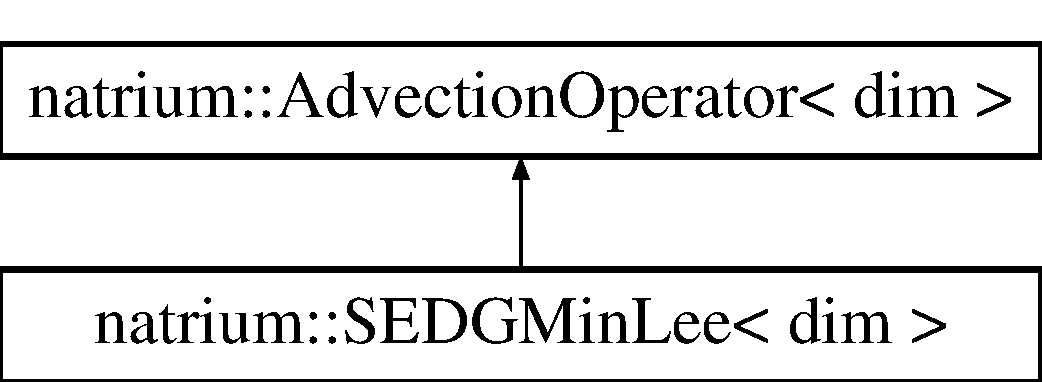
\includegraphics[height=2.000000cm]{classnatrium_1_1AdvectionOperator}
\end{center}
\end{figure}
\subsection*{Public Member Functions}
\begin{DoxyCompactItemize}
\item 
\hypertarget{classnatrium_1_1AdvectionOperator_a48d3a57e3433d9f6c3768ad2f392df56}{\hyperlink{classnatrium_1_1AdvectionOperator_a48d3a57e3433d9f6c3768ad2f392df56}{Advection\-Operator} ()}\label{classnatrium_1_1AdvectionOperator_a48d3a57e3433d9f6c3768ad2f392df56}

\begin{DoxyCompactList}\small\item\em constructor \end{DoxyCompactList}\item 
\hypertarget{classnatrium_1_1AdvectionOperator_a691156dace41e3075fd89953f30ae83f}{virtual \hyperlink{classnatrium_1_1AdvectionOperator_a691156dace41e3075fd89953f30ae83f}{$\sim$\-Advection\-Operator} ()}\label{classnatrium_1_1AdvectionOperator_a691156dace41e3075fd89953f30ae83f}

\begin{DoxyCompactList}\small\item\em destructor \end{DoxyCompactList}\item 
\hypertarget{classnatrium_1_1AdvectionOperator_a89c25c3dae9a1e5973cd89fab8c2c052}{virtual void \hyperlink{classnatrium_1_1AdvectionOperator_a89c25c3dae9a1e5973cd89fab8c2c052}{reassemble} ()=0}\label{classnatrium_1_1AdvectionOperator_a89c25c3dae9a1e5973cd89fab8c2c052}

\begin{DoxyCompactList}\small\item\em function to (re-\/)assemble linear system \end{DoxyCompactList}\item 
\hypertarget{classnatrium_1_1AdvectionOperator_aacdf6096f40166c5ec64686655c906a0}{virtual void \hyperlink{classnatrium_1_1AdvectionOperator_aacdf6096f40166c5ec64686655c906a0}{stream} ()=0}\label{classnatrium_1_1AdvectionOperator_aacdf6096f40166c5ec64686655c906a0}

\begin{DoxyCompactList}\small\item\em make streaming step \end{DoxyCompactList}\item 
\hypertarget{classnatrium_1_1AdvectionOperator_a2cbaee43740d976492e6c9d6d2b84ad0}{virtual const \\*
distributed\-\_\-sparse\-\_\-block\-\_\-matrix \& {\bfseries get\-System\-Matrix} () const =0}\label{classnatrium_1_1AdvectionOperator_a2cbaee43740d976492e6c9d6d2b84ad0}

\item 
\hypertarget{classnatrium_1_1AdvectionOperator_a68f51edd8cc34b61f32ded0a8db82f7b}{virtual const shared\-\_\-ptr\\*
$<$ dealii\-::\-Do\-F\-Handler$<$ dim $>$ $>$ \& {\bfseries get\-Do\-F\-Handler} () const =0}\label{classnatrium_1_1AdvectionOperator_a68f51edd8cc34b61f32ded0a8db82f7b}

\item 
\hypertarget{classnatrium_1_1AdvectionOperator_adc118010e30df45b5906d35743e5ec2e}{virtual void {\bfseries map\-Do\-Fs\-To\-Support\-Points} (vector$<$ dealii\-::\-Point$<$ dim $>$ $>$ \&support\-Points) const =0}\label{classnatrium_1_1AdvectionOperator_adc118010e30df45b5906d35743e5ec2e}

\item 
\hypertarget{classnatrium_1_1AdvectionOperator_a419e94f5534d7871cee47c027a2501c4}{virtual const \\*
dealii\-::\-Mapping\-Q1$<$ dim $>$ \& {\bfseries get\-Mapping} () const =0}\label{classnatrium_1_1AdvectionOperator_a419e94f5534d7871cee47c027a2501c4}

\item 
virtual void \hyperlink{classnatrium_1_1AdvectionOperator_aca14260bae100874b0050a2a96d7a564}{save\-Checkpoint} (const string \&directory) const =0
\begin{DoxyCompactList}\small\item\em save matrices and status to files \end{DoxyCompactList}\item 
\hypertarget{classnatrium_1_1AdvectionOperator_a251e21d1dd023926d4c5f7fd973b90bf}{virtual size\-\_\-t {\bfseries get\-Number\-Of\-Do\-Fs} () const =0}\label{classnatrium_1_1AdvectionOperator_a251e21d1dd023926d4c5f7fd973b90bf}

\end{DoxyCompactItemize}


\subsection{Detailed Description}
\subsubsection*{template$<$size\-\_\-t dim$>$class natrium\-::\-Advection\-Operator$<$ dim $>$}

Abstract class for spatial part of the Advection Operator e\-\_\-i $\ast$ dx\-\_\-i f. 


\begin{DoxyTemplParams}{Template Parameters}
{\em dim} & The dimension of the flow (2 or 3). \\
\hline
\end{DoxyTemplParams}


\subsection{Member Function Documentation}
\hypertarget{classnatrium_1_1AdvectionOperator_aca14260bae100874b0050a2a96d7a564}{\index{natrium\-::\-Advection\-Operator@{natrium\-::\-Advection\-Operator}!save\-Checkpoint@{save\-Checkpoint}}
\index{save\-Checkpoint@{save\-Checkpoint}!natrium::AdvectionOperator@{natrium\-::\-Advection\-Operator}}
\subsubsection[{save\-Checkpoint}]{\setlength{\rightskip}{0pt plus 5cm}template$<$size\-\_\-t dim$>$ virtual void {\bf natrium\-::\-Advection\-Operator}$<$ dim $>$\-::save\-Checkpoint (
\begin{DoxyParamCaption}
\item[{const string \&}]{directory}
\end{DoxyParamCaption}
) const\hspace{0.3cm}{\ttfamily [pure virtual]}}}\label{classnatrium_1_1AdvectionOperator_aca14260bae100874b0050a2a96d7a564}


save matrices and status to files 


\begin{DoxyParams}[1]{Parameters}
\mbox{\tt in}  & {\em directory} & directory to save the matrix files to \\
\hline
\end{DoxyParams}

\begin{DoxyExceptions}{Exceptions}
{\em \hyperlink{classnatrium_1_1AdvectionSolverException}{Advection\-Solver\-Exception}} & \\
\hline
\end{DoxyExceptions}


Implemented in \hyperlink{classnatrium_1_1SEDGMinLee_ab3cf80e18230ee7f08f4ed9883b9dadd}{natrium\-::\-S\-E\-D\-G\-Min\-Lee$<$ dim $>$}.



The documentation for this class was generated from the following file\-:\begin{DoxyCompactItemize}
\item 
/home/kraemer/eclipse\-\_\-workspace/\-N\-A\-Triu\-M/src/natrium/advection/\hyperlink{AdvectionOperator_8h}{Advection\-Operator.\-h}\end{DoxyCompactItemize}

\hypertarget{classnatrium_1_1AdvectionSolverException}{
\section{natrium::AdvectionSolverException Class Reference}
\label{classnatrium_1_1AdvectionSolverException}\index{natrium::AdvectionSolverException@{natrium::AdvectionSolverException}}
}


Exception class for \hyperlink{classnatrium_1_1AdvectionOperator}{AdvectionOperator}.  


{\ttfamily \#include $<$AdvectionTools.h$>$}Inheritance diagram for natrium::AdvectionSolverException::\begin{figure}[H]
\begin{center}
\leavevmode
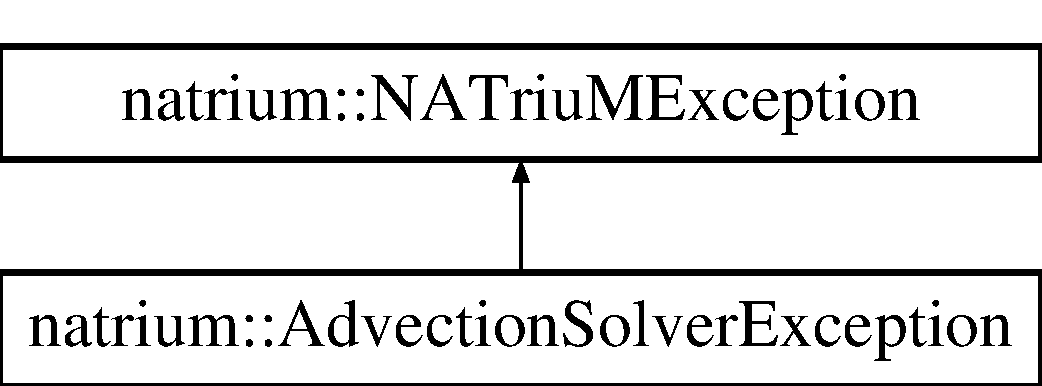
\includegraphics[height=2cm]{classnatrium_1_1AdvectionSolverException}
\end{center}
\end{figure}
\subsection*{Public Member Functions}
\begin{DoxyCompactItemize}
\item 
\hypertarget{classnatrium_1_1AdvectionSolverException_a443084a12dee879bdfbfc900202a0706}{
{\bfseries AdvectionSolverException} (const char $\ast$msg)}
\label{classnatrium_1_1AdvectionSolverException_a443084a12dee879bdfbfc900202a0706}

\item 
\hypertarget{classnatrium_1_1AdvectionSolverException_a9cda3faa279e3528f96c3780a91545bd}{
{\bfseries AdvectionSolverException} (const string \&msg)}
\label{classnatrium_1_1AdvectionSolverException_a9cda3faa279e3528f96c3780a91545bd}

\item 
\hypertarget{classnatrium_1_1AdvectionSolverException_aeb13fafe3f75de7cfd4e282a8a0fb5b0}{
const char $\ast$ {\bfseries what} () const   throw ()}
\label{classnatrium_1_1AdvectionSolverException_aeb13fafe3f75de7cfd4e282a8a0fb5b0}

\end{DoxyCompactItemize}


\subsection{Detailed Description}
Exception class for \hyperlink{classnatrium_1_1AdvectionOperator}{AdvectionOperator}. 

The documentation for this class was generated from the following file:\begin{DoxyCompactItemize}
\item 
/mnt/fdrive/akraem3m/workspace/NATriuM/src/library/natrium/advection/AdvectionTools.h\end{DoxyCompactItemize}

\hypertarget{classnatrium_1_1Benchmark}{
\section{natrium::Benchmark$<$ dim $>$ Class Template Reference}
\label{classnatrium_1_1Benchmark}\index{natrium::Benchmark@{natrium::Benchmark}}
}
Inheritance diagram for natrium::Benchmark$<$ dim $>$::\begin{figure}[H]
\begin{center}
\leavevmode
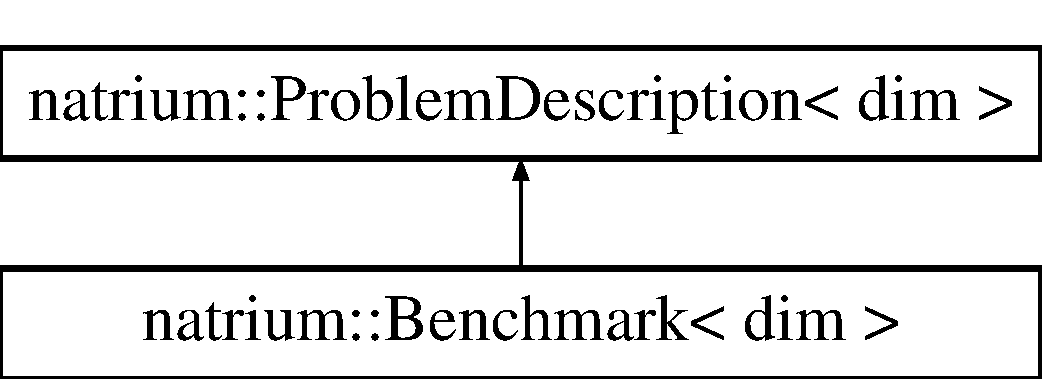
\includegraphics[height=2cm]{classnatrium_1_1Benchmark}
\end{center}
\end{figure}
\subsection*{Public Member Functions}
\begin{DoxyCompactItemize}
\item 
\hypertarget{classnatrium_1_1Benchmark_afad7bc0117bd13bf116d8b00518b774e}{
\hyperlink{classnatrium_1_1Benchmark_afad7bc0117bd13bf116d8b00518b774e}{Benchmark} (shared\_\-ptr$<$ Mesh$<$ dim $>$ $>$ triangulation, double viscosity, double characteristicLength)}
\label{classnatrium_1_1Benchmark_afad7bc0117bd13bf116d8b00518b774e}

\begin{DoxyCompactList}\small\item\em Constructor. \item\end{DoxyCompactList}\item 
\hypertarget{classnatrium_1_1Benchmark_a9560e49a097a369ec972b72fb2873a2e}{
virtual \hyperlink{classnatrium_1_1Benchmark_a9560e49a097a369ec972b72fb2873a2e}{$\sim$Benchmark} ()}
\label{classnatrium_1_1Benchmark_a9560e49a097a369ec972b72fb2873a2e}

\begin{DoxyCompactList}\small\item\em Destructor. \item\end{DoxyCompactList}\item 
\hypertarget{classnatrium_1_1Benchmark_a21e67666e47f219a441bb80697e23b63}{
const shared\_\-ptr$<$ dealii::Function$<$ dim $>$ $>$ \& {\bfseries getAnalyticRhoFunction} (double time) const }
\label{classnatrium_1_1Benchmark_a21e67666e47f219a441bb80697e23b63}

\item 
\hypertarget{classnatrium_1_1Benchmark_a398e571355ecd6a95c7f7d40cf19c783}{
const shared\_\-ptr$<$ dealii::Function$<$ dim $>$ $>$ \& {\bfseries getAnalyticUFunction} (double time) const }
\label{classnatrium_1_1Benchmark_a398e571355ecd6a95c7f7d40cf19c783}

\item 
\hypertarget{classnatrium_1_1Benchmark_a720202a91c6777d3196415fe0c1f86ea}{
virtual const shared\_\-ptr$<$ dealii::Function$<$ dim $>$ $>$ \& {\bfseries getInitialRhoFunction} () const }
\label{classnatrium_1_1Benchmark_a720202a91c6777d3196415fe0c1f86ea}

\item 
\hypertarget{classnatrium_1_1Benchmark_ae2b476e376bd1d87f754e0acdfdc1e0e}{
virtual const shared\_\-ptr$<$ dealii::Function$<$ dim $>$ $>$ \& {\bfseries getInitialUFunction} () const }
\label{classnatrium_1_1Benchmark_ae2b476e376bd1d87f754e0acdfdc1e0e}

\end{DoxyCompactItemize}
\subsection*{Protected Member Functions}
\begin{DoxyCompactItemize}
\item 
\hypertarget{classnatrium_1_1Benchmark_a5232102078b3d709cf9c8a79be391ddf}{
void {\bfseries setAnalyticRho} (shared\_\-ptr$<$ dealii::Function$<$ dim $>$ $>$ ana\_\-rho)}
\label{classnatrium_1_1Benchmark_a5232102078b3d709cf9c8a79be391ddf}

\item 
\hypertarget{classnatrium_1_1Benchmark_ac61be28bab79a44b4ff32c20f6d92483}{
void {\bfseries setAnalyticU} (shared\_\-ptr$<$ dealii::Function$<$ dim $>$ $>$ ana\_\-u)}
\label{classnatrium_1_1Benchmark_ac61be28bab79a44b4ff32c20f6d92483}

\end{DoxyCompactItemize}
\subsubsection*{template$<$size\_\-t dim$>$ class natrium::Benchmark$<$ dim $>$}



The documentation for this class was generated from the following file:\begin{DoxyCompactItemize}
\item 
/mnt/fdrive/akraem3m/workspace/NATriuM/src/library/natrium/problemdescription/\hyperlink{Benchmark_8h}{Benchmark.h}\end{DoxyCompactItemize}

\hypertarget{classnatrium_1_1BenchmarkCFDSolver}{\section{natrium\-:\-:Benchmark\-C\-F\-D\-Solver$<$ dim $>$ Class Template Reference}
\label{classnatrium_1_1BenchmarkCFDSolver}\index{natrium\-::\-Benchmark\-C\-F\-D\-Solver$<$ dim $>$@{natrium\-::\-Benchmark\-C\-F\-D\-Solver$<$ dim $>$}}
}


a class that overrides the output function of the C\-F\-D solver class with comparisons to a reference solution  




{\ttfamily \#include $<$Benchmark\-C\-F\-D\-Solver.\-h$>$}

Inheritance diagram for natrium\-:\-:Benchmark\-C\-F\-D\-Solver$<$ dim $>$\-:\begin{figure}[H]
\begin{center}
\leavevmode
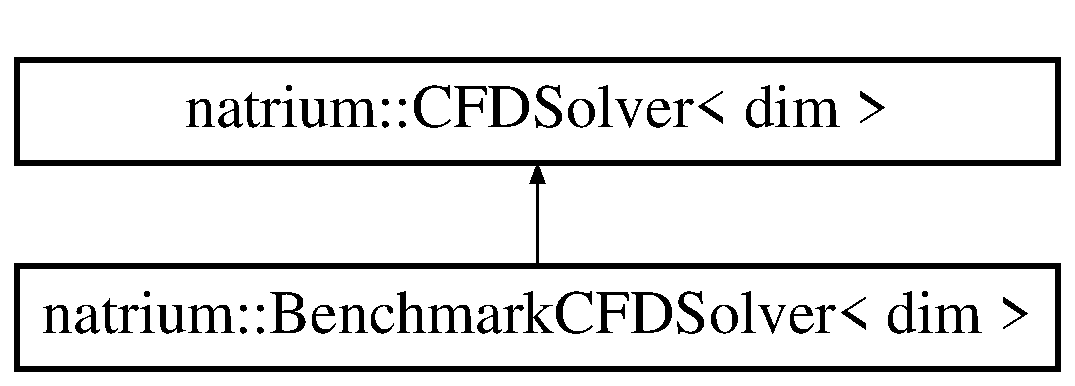
\includegraphics[height=2.000000cm]{classnatrium_1_1BenchmarkCFDSolver}
\end{center}
\end{figure}
\subsection*{Public Member Functions}
\begin{DoxyCompactItemize}
\item 
\hypertarget{classnatrium_1_1BenchmarkCFDSolver_ac90d82e4b09e658a18439996b0ab1ec1}{\hyperlink{classnatrium_1_1BenchmarkCFDSolver_ac90d82e4b09e658a18439996b0ab1ec1}{Benchmark\-C\-F\-D\-Solver} (shared\-\_\-ptr$<$ \hyperlink{classnatrium_1_1SolverConfiguration}{Solver\-Configuration} $>$ configuration, shared\-\_\-ptr$<$ \hyperlink{classnatrium_1_1Benchmark}{Benchmark}$<$ dim $>$ $>$ problem\-Description)}\label{classnatrium_1_1BenchmarkCFDSolver_ac90d82e4b09e658a18439996b0ab1ec1}

\begin{DoxyCompactList}\small\item\em constructor \end{DoxyCompactList}\item 
\hypertarget{classnatrium_1_1BenchmarkCFDSolver_a9708132fc0cef4ae55e3453672891c81}{virtual void \hyperlink{classnatrium_1_1BenchmarkCFDSolver_a9708132fc0cef4ae55e3453672891c81}{output} (size\-\_\-t iteration)}\label{classnatrium_1_1BenchmarkCFDSolver_a9708132fc0cef4ae55e3453672891c81}

\begin{DoxyCompactList}\small\item\em create output data and write to file \end{DoxyCompactList}\item 
\hypertarget{classnatrium_1_1BenchmarkCFDSolver_a96be8add7c888ef4e6a1cb41cd2b40f6}{virtual void \hyperlink{classnatrium_1_1BenchmarkCFDSolver_a96be8add7c888ef4e6a1cb41cd2b40f6}{add\-Analytic\-Solution\-To\-Output} (dealii\-::\-Data\-Out$<$ dim $>$ \&data\-\_\-out)}\label{classnatrium_1_1BenchmarkCFDSolver_a96be8add7c888ef4e6a1cb41cd2b40f6}

\begin{DoxyCompactList}\small\item\em gives the possibility for \hyperlink{classnatrium_1_1Benchmark}{Benchmark} instances to add the analytic solution to output \end{DoxyCompactList}\item 
\hypertarget{classnatrium_1_1BenchmarkCFDSolver_aafd3c01db648420ce6d98a8349bdfa09}{virtual \hyperlink{classnatrium_1_1BenchmarkCFDSolver_aafd3c01db648420ce6d98a8349bdfa09}{$\sim$\-Benchmark\-C\-F\-D\-Solver} ()}\label{classnatrium_1_1BenchmarkCFDSolver_aafd3c01db648420ce6d98a8349bdfa09}

\begin{DoxyCompactList}\small\item\em destructor \end{DoxyCompactList}\item 
\hypertarget{classnatrium_1_1BenchmarkCFDSolver_a3c2c8da9004e370209db1b611a136fe9}{const distributed\-\_\-vector \& {\bfseries get\-Analytic\-Density} () const }\label{classnatrium_1_1BenchmarkCFDSolver_a3c2c8da9004e370209db1b611a136fe9}

\item 
\hypertarget{classnatrium_1_1BenchmarkCFDSolver_aee14ac9e3a9d36960d16f0b4899a3c08}{const vector\\*
$<$ distributed\-\_\-vector $>$ \& {\bfseries get\-Analytic\-Velocity} () const }\label{classnatrium_1_1BenchmarkCFDSolver_aee14ac9e3a9d36960d16f0b4899a3c08}

\item 
\hypertarget{classnatrium_1_1BenchmarkCFDSolver_aa5a174cf76431ba7b1721f1ce55df967}{const shared\-\_\-ptr$<$ \hyperlink{classnatrium_1_1Benchmark}{Benchmark}\\*
$<$ dim $>$ $>$ \& {\bfseries get\-Benchmark} () const }\label{classnatrium_1_1BenchmarkCFDSolver_aa5a174cf76431ba7b1721f1ce55df967}

\item 
\hypertarget{classnatrium_1_1BenchmarkCFDSolver_a7d71686aaf03be14827bded582f76e71}{const vector$<$ dealii\-::\-Point$<$ 2 $>$ $>$ \& {\bfseries get\-Support\-Points} () const }\label{classnatrium_1_1BenchmarkCFDSolver_a7d71686aaf03be14827bded582f76e71}

\item 
\hypertarget{classnatrium_1_1BenchmarkCFDSolver_ac015d170b19024e63ff43f4a2e516fef}{const shared\-\_\-ptr$<$ \hyperlink{classnatrium_1_1ErrorStats}{Error\-Stats}\\*
$<$ dim $>$ $>$ \& {\bfseries get\-Error\-Stats} () const }\label{classnatrium_1_1BenchmarkCFDSolver_ac015d170b19024e63ff43f4a2e516fef}

\end{DoxyCompactItemize}
\subsection*{Friends}
\begin{DoxyCompactItemize}
\item 
\hypertarget{classnatrium_1_1BenchmarkCFDSolver_af0f098157b0009154b8effd1fb919fe6}{{\footnotesize template$<$size\-\_\-t dim2$>$ }\\class {\bfseries Error\-Stats}}\label{classnatrium_1_1BenchmarkCFDSolver_af0f098157b0009154b8effd1fb919fe6}

\end{DoxyCompactItemize}
\subsection*{Additional Inherited Members}


\subsection{Detailed Description}
\subsubsection*{template$<$size\-\_\-t dim$>$class natrium\-::\-Benchmark\-C\-F\-D\-Solver$<$ dim $>$}

a class that overrides the output function of the C\-F\-D solver class with comparisons to a reference solution 

The documentation for this class was generated from the following files\-:\begin{DoxyCompactItemize}
\item 
/home/kraemer/eclipse\-\_\-workspace/\-N\-A\-Triu\-M/src/natrium/solver/Benchmark\-C\-F\-D\-Solver.\-h\item 
/home/kraemer/eclipse\-\_\-workspace/\-N\-A\-Triu\-M/src/natrium/solver/Benchmark\-C\-F\-D\-Solver.\-cpp\end{DoxyCompactItemize}

\hypertarget{classnatrium_1_1BGKTransformed}{\section{natrium\-:\-:B\-G\-K\-Transformed Class Reference}
\label{classnatrium_1_1BGKTransformed}\index{natrium\-::\-B\-G\-K\-Transformed@{natrium\-::\-B\-G\-K\-Transformed}}
}


Description of the B\-G\-K model for the transformed particle distributions, as described in Global data which is used by Min and Lee (2011)\-: A spectral-\/element discontinuous Galerkin lattice Boltzmann method for nearly incompressible flows, J\-C\-P 230 pp. 245-\/259.  




{\ttfamily \#include $<$B\-G\-K\-Transformed.\-h$>$}

Inheritance diagram for natrium\-:\-:B\-G\-K\-Transformed\-:\begin{figure}[H]
\begin{center}
\leavevmode
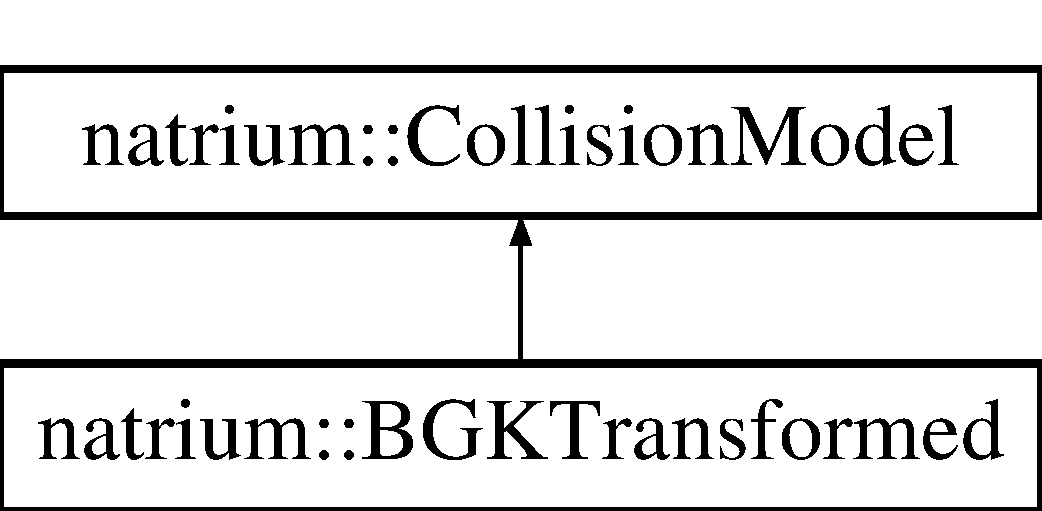
\includegraphics[height=2.000000cm]{classnatrium_1_1BGKTransformed}
\end{center}
\end{figure}
\subsection*{Public Member Functions}
\begin{DoxyCompactItemize}
\item 
\hyperlink{classnatrium_1_1BGKTransformed_aafd0ed5b888da93e496c0a29e092bf5b}{B\-G\-K\-Transformed} (double relaxation\-Parameter, boost\-::shared\-\_\-ptr$<$ \hyperlink{classnatrium_1_1BoltzmannModel}{Boltzmann\-Model} $>$ boltzmann\-Model)
\begin{DoxyCompactList}\small\item\em constructor \end{DoxyCompactList}\item 
\hypertarget{classnatrium_1_1BGKTransformed_a554c68facfbd2b126f24504f215eb193}{virtual \hyperlink{classnatrium_1_1BGKTransformed_a554c68facfbd2b126f24504f215eb193}{$\sim$\-B\-G\-K\-Transformed} ()}\label{classnatrium_1_1BGKTransformed_a554c68facfbd2b126f24504f215eb193}

\begin{DoxyCompactList}\small\item\em destructor \end{DoxyCompactList}\item 
virtual void \hyperlink{classnatrium_1_1BGKTransformed_a2e40159e5f5204431b1acb84b15910c0}{collide\-Single\-Point} (vector$<$ double $>$ \&distributions) const 
\begin{DoxyCompactList}\small\item\em function for collision \end{DoxyCompactList}\item 
virtual void \hyperlink{classnatrium_1_1BGKTransformed_a6bb41acd37234d2f92a9d868ff2486e1}{collide\-Single\-Do\-F} (size\-\_\-t do\-F, const vector$<$ double $>$ \&feq, \hyperlink{classnatrium_1_1DistributionFunctions}{Distribution\-Functions} \&f) const 
\begin{DoxyCompactList}\small\item\em virtual function for collision \end{DoxyCompactList}\end{DoxyCompactItemize}
\subsection*{Additional Inherited Members}


\subsection{Detailed Description}
Description of the B\-G\-K model for the transformed particle distributions, as described in Global data which is used by Min and Lee (2011)\-: A spectral-\/element discontinuous Galerkin lattice Boltzmann method for nearly incompressible flows, J\-C\-P 230 pp. 245-\/259. 

\subsection{Constructor \& Destructor Documentation}
\hypertarget{classnatrium_1_1BGKTransformed_aafd0ed5b888da93e496c0a29e092bf5b}{\index{natrium\-::\-B\-G\-K\-Transformed@{natrium\-::\-B\-G\-K\-Transformed}!B\-G\-K\-Transformed@{B\-G\-K\-Transformed}}
\index{B\-G\-K\-Transformed@{B\-G\-K\-Transformed}!natrium::BGKTransformed@{natrium\-::\-B\-G\-K\-Transformed}}
\subsubsection[{B\-G\-K\-Transformed}]{\setlength{\rightskip}{0pt plus 5cm}natrium\-::\-B\-G\-K\-Transformed\-::\-B\-G\-K\-Transformed (
\begin{DoxyParamCaption}
\item[{double}]{relaxation\-Parameter, }
\item[{boost\-::shared\-\_\-ptr$<$ {\bf Boltzmann\-Model} $>$}]{boltzmann\-Model}
\end{DoxyParamCaption}
)}}\label{classnatrium_1_1BGKTransformed_aafd0ed5b888da93e496c0a29e092bf5b}


constructor 


\begin{DoxyParams}[1]{Parameters}
\mbox{\tt in}  & {\em relaxation\-Parameter} & relaxation parameter tau \\
\hline
\end{DoxyParams}


\subsection{Member Function Documentation}
\hypertarget{classnatrium_1_1BGKTransformed_a6bb41acd37234d2f92a9d868ff2486e1}{\index{natrium\-::\-B\-G\-K\-Transformed@{natrium\-::\-B\-G\-K\-Transformed}!collide\-Single\-Do\-F@{collide\-Single\-Do\-F}}
\index{collide\-Single\-Do\-F@{collide\-Single\-Do\-F}!natrium::BGKTransformed@{natrium\-::\-B\-G\-K\-Transformed}}
\subsubsection[{collide\-Single\-Do\-F}]{\setlength{\rightskip}{0pt plus 5cm}void natrium\-::\-B\-G\-K\-Transformed\-::collide\-Single\-Do\-F (
\begin{DoxyParamCaption}
\item[{size\-\_\-t}]{do\-F, }
\item[{const vector$<$ double $>$ \&}]{feq, }
\item[{{\bf Distribution\-Functions} \&}]{f}
\end{DoxyParamCaption}
) const\hspace{0.3cm}{\ttfamily [virtual]}}}\label{classnatrium_1_1BGKTransformed_a6bb41acd37234d2f92a9d868ff2486e1}


virtual function for collision 


\begin{DoxyParams}[1]{Parameters}
\mbox{\tt in}  & {\em do\-F} & the do\-F index for which collision is done \\
\hline
\mbox{\tt in}  & {\em feq} & the vector of local equilibrium distributions \\
\hline
\mbox{\tt in}  & {\em f} & the vector of global distribution functions \\
\hline
\end{DoxyParams}


Implements \hyperlink{classnatrium_1_1CollisionModel_abe4f58658074680b679db7b7fddd6113}{natrium\-::\-Collision\-Model}.

\hypertarget{classnatrium_1_1BGKTransformed_a2e40159e5f5204431b1acb84b15910c0}{\index{natrium\-::\-B\-G\-K\-Transformed@{natrium\-::\-B\-G\-K\-Transformed}!collide\-Single\-Point@{collide\-Single\-Point}}
\index{collide\-Single\-Point@{collide\-Single\-Point}!natrium::BGKTransformed@{natrium\-::\-B\-G\-K\-Transformed}}
\subsubsection[{collide\-Single\-Point}]{\setlength{\rightskip}{0pt plus 5cm}void natrium\-::\-B\-G\-K\-Transformed\-::collide\-Single\-Point (
\begin{DoxyParamCaption}
\item[{vector$<$ double $>$ \&}]{distributions}
\end{DoxyParamCaption}
) const\hspace{0.3cm}{\ttfamily [virtual]}}}\label{classnatrium_1_1BGKTransformed_a2e40159e5f5204431b1acb84b15910c0}


function for collision 


\begin{DoxyParams}{Parameters}
{\em in/out\mbox{]}} & distributions the particle distribution functions \\
\hline
\end{DoxyParams}


Implements \hyperlink{classnatrium_1_1CollisionModel_acde767e924eb2124ab3eb725543111e8}{natrium\-::\-Collision\-Model}.



The documentation for this class was generated from the following files\-:\begin{DoxyCompactItemize}
\item 
/home/kraemer/eclipse\-\_\-workspace/\-N\-A\-Triu\-M/src/natrium/collisionmodels/\hyperlink{BGKTransformed_8h}{B\-G\-K\-Transformed.\-h}\item 
/home/kraemer/eclipse\-\_\-workspace/\-N\-A\-Triu\-M/src/natrium/collisionmodels/\hyperlink{BGKTransformed_8cpp}{B\-G\-K\-Transformed.\-cpp}\end{DoxyCompactItemize}

\hypertarget{classnatrium_1_1BoltzmannModel}{\section{natrium\-:\-:\-Boltzmann\-Model \-Class \-Reference}
\label{classnatrium_1_1BoltzmannModel}\index{natrium\-::\-Boltzmann\-Model@{natrium\-::\-Boltzmann\-Model}}
}


\-Abstract class for the description of a boltzmann model, e.\-g. \-D2\-Q9.  




{\ttfamily \#include $<$\-Boltzmann\-Model.\-h$>$}

\-Inheritance diagram for natrium\-:\-:\-Boltzmann\-Model\-:\begin{figure}[H]
\begin{center}
\leavevmode
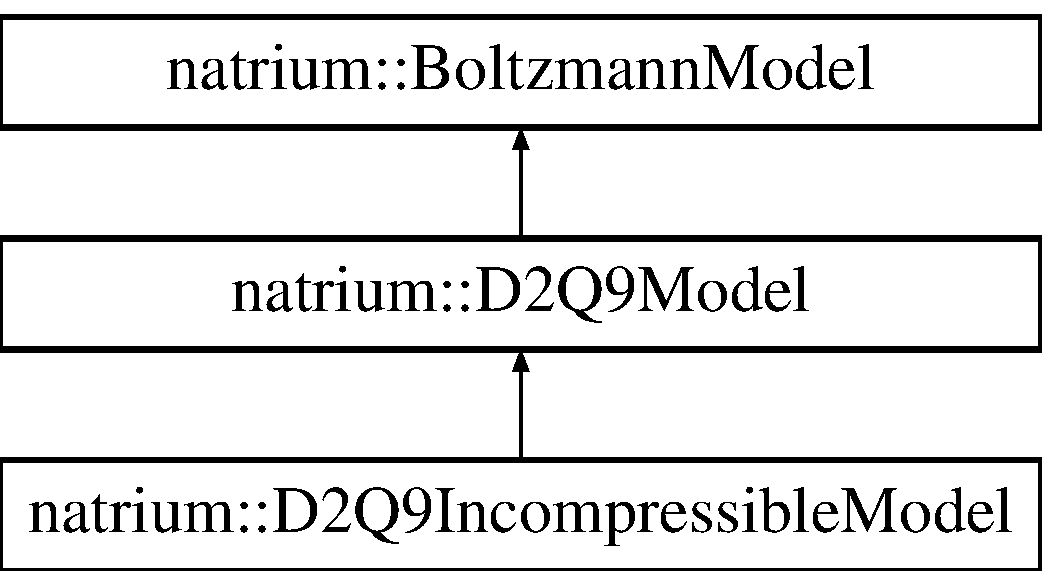
\includegraphics[height=3.000000cm]{classnatrium_1_1BoltzmannModel}
\end{center}
\end{figure}
\subsection*{\-Public \-Member \-Functions}
\begin{DoxyCompactItemize}
\item 
\hyperlink{classnatrium_1_1BoltzmannModel_a0547ee3c88330d7a2ac44ad3ece8d560}{\-Boltzmann\-Model} (size\-\_\-t d, size\-\_\-t q, const vector$<$ numeric\-\_\-vector $>$ \&directions, const vector$<$ float\-\_\-t $>$ \&weights, \-Stencil\-Type stencil\-Type)
\begin{DoxyCompactList}\small\item\em constructor \end{DoxyCompactList}\item 
\hypertarget{classnatrium_1_1BoltzmannModel_ac2e3dabcbe15c1e37ff09ec1c53dafa5}{virtual \hyperlink{classnatrium_1_1BoltzmannModel_ac2e3dabcbe15c1e37ff09ec1c53dafa5}{$\sim$\-Boltzmann\-Model} ()}\label{classnatrium_1_1BoltzmannModel_ac2e3dabcbe15c1e37ff09ec1c53dafa5}

\begin{DoxyCompactList}\small\item\em destructor \end{DoxyCompactList}\item 
const vector$<$ numeric\-\_\-vector $>$ \& \hyperlink{classnatrium_1_1BoltzmannModel_aeabed4142acd04a57ba41ca26dfbe666}{get\-Directions} () const 
\begin{DoxyCompactList}\small\item\em get a reference to the vector of directions \end{DoxyCompactList}\item 
const numeric\-\_\-vector \& \hyperlink{classnatrium_1_1BoltzmannModel_a0b258b2c7cc4cba5ac666a06ca2a8f49}{get\-Direction} (size\-\_\-t i) const 
\begin{DoxyCompactList}\small\item\em get the i-\/th direction \end{DoxyCompactList}\item 
size\-\_\-t \hyperlink{classnatrium_1_1BoltzmannModel_ae7cfcd108a085d3215cdc8c00e826107}{get\-Q} () const 
\begin{DoxyCompactList}\small\item\em get q, the number of directions in the \-Dd\-Qq-\/stencil \end{DoxyCompactList}\item 
size\-\_\-t \hyperlink{classnatrium_1_1BoltzmannModel_a8d16745a0dab65cb0324d6b076e53d15}{get\-D} () const 
\begin{DoxyCompactList}\small\item\em get d, the dimension of the \-Dd\-Qq-\/stencil \end{DoxyCompactList}\item 
const vector$<$ float\-\_\-t $>$ \& \hyperlink{classnatrium_1_1BoltzmannModel_a3158e70071707c169486d87d26727f3c}{get\-Weights} () const 
\begin{DoxyCompactList}\small\item\em get the weights of the equilibrium distributions \end{DoxyCompactList}\item 
float\-\_\-t \hyperlink{classnatrium_1_1BoltzmannModel_aae549c1f5dd48a92fc9e174afc5de1a5}{get\-Weight} (size\-\_\-t i) const 
\begin{DoxyCompactList}\small\item\em get the weight belonging to a certain direction \end{DoxyCompactList}\item 
const \-Stencil\-Type \hyperlink{classnatrium_1_1BoltzmannModel_ac95c2547a37e380d8d7b3de3c0f8a4c2}{get\-Stencil\-Type} () const 
\begin{DoxyCompactList}\small\item\em get stencil type \end{DoxyCompactList}\item 
float\-\_\-t \hyperlink{classnatrium_1_1BoltzmannModel_adf8901da899eef5d11b0cbf80200ee32}{calculate\-Density} (const vector$<$ float\-\_\-t $>$ \&distributions) const 
\begin{DoxyCompactList}\small\item\em calculate macroscopic density \end{DoxyCompactList}\item 
numeric\-\_\-vector \hyperlink{classnatrium_1_1BoltzmannModel_a2c7e3465bb3541e420f15a7970533047}{calculate\-Velocity} (const vector$<$ float\-\_\-t $>$ \&distributions) const 
\begin{DoxyCompactList}\small\item\em calculate macroscopic velocity \end{DoxyCompactList}\item 
void \hyperlink{classnatrium_1_1BoltzmannModel_a3d5a504ad3dc0b3847c5db412b1988b8}{calculate\-Velocity} (const vector$<$ float\-\_\-t $>$ \&distributions, const float\-\_\-t rho, numeric\-\_\-vector \&u) const 
\begin{DoxyCompactList}\small\item\em calculate macroscopic velocity; saves the double calculation of the density \end{DoxyCompactList}\item 
virtual float\-\_\-t \hyperlink{classnatrium_1_1BoltzmannModel_ac5615f43cd5c03c881734d4826ce31be}{get\-Equilibrium\-Distribution} (size\-\_\-t i, const numeric\-\_\-vector \&u, const float\-\_\-t rho=1) const =0
\begin{DoxyCompactList}\small\item\em virtual function for the calculation of the equilibrium distribution \end{DoxyCompactList}\item 
virtual void \hyperlink{classnatrium_1_1BoltzmannModel_aab8d824211e65a394536333c5537b325}{get\-Equilibrium\-Distributions} (vector$<$ float\-\_\-t $>$ \&feq, const numeric\-\_\-vector \&u, const float\-\_\-t rho=1) const 
\begin{DoxyCompactList}\small\item\em function for the calculation of all equilibrium distributions \end{DoxyCompactList}\end{DoxyCompactItemize}


\subsection{\-Detailed \-Description}
\-Abstract class for the description of a boltzmann model, e.\-g. \-D2\-Q9. 

\subsection{\-Constructor \& \-Destructor \-Documentation}
\hypertarget{classnatrium_1_1BoltzmannModel_a0547ee3c88330d7a2ac44ad3ece8d560}{\index{natrium\-::\-Boltzmann\-Model@{natrium\-::\-Boltzmann\-Model}!\-Boltzmann\-Model@{\-Boltzmann\-Model}}
\index{\-Boltzmann\-Model@{\-Boltzmann\-Model}!natrium::BoltzmannModel@{natrium\-::\-Boltzmann\-Model}}
\subsubsection[{\-Boltzmann\-Model}]{\setlength{\rightskip}{0pt plus 5cm}{\bf natrium\-::\-Boltzmann\-Model\-::\-Boltzmann\-Model} (
\begin{DoxyParamCaption}
\item[{size\-\_\-t}]{d, }
\item[{size\-\_\-t}]{q, }
\item[{const vector$<$ numeric\-\_\-vector $>$ \&}]{directions, }
\item[{const vector$<$ float\-\_\-t $>$ \&}]{weights, }
\item[{\-Stencil\-Type}]{stencil\-Type}
\end{DoxyParamCaption}
)}}\label{classnatrium_1_1BoltzmannModel_a0547ee3c88330d7a2ac44ad3ece8d560}


constructor 


\begin{DoxyParams}{\-Parameters}
{\em d} & dimension \\
\hline
{\em q} & number of directions \\
\hline
{\em directions} & the directions of the stencil \\
\hline
{\em weights} & the weights of the equilibrium distribution \\
\hline
{\em stencil\-Type} & type of the stencil (e.\-g. \-D2\-Q9) \\
\hline
\end{DoxyParams}


\subsection{\-Member \-Function \-Documentation}
\hypertarget{classnatrium_1_1BoltzmannModel_adf8901da899eef5d11b0cbf80200ee32}{\index{natrium\-::\-Boltzmann\-Model@{natrium\-::\-Boltzmann\-Model}!calculate\-Density@{calculate\-Density}}
\index{calculate\-Density@{calculate\-Density}!natrium::BoltzmannModel@{natrium\-::\-Boltzmann\-Model}}
\subsubsection[{calculate\-Density}]{\setlength{\rightskip}{0pt plus 5cm}float\-\_\-t {\bf natrium\-::\-Boltzmann\-Model\-::calculate\-Density} (
\begin{DoxyParamCaption}
\item[{const vector$<$ float\-\_\-t $>$ \&}]{distributions}
\end{DoxyParamCaption}
) const\hspace{0.3cm}{\ttfamily  \mbox{[}inline\mbox{]}}}}\label{classnatrium_1_1BoltzmannModel_adf8901da899eef5d11b0cbf80200ee32}


calculate macroscopic density 


\begin{DoxyParams}[1]{\-Parameters}
\mbox{\tt in}  & {\em distributions} & particle distribution functions at a given point \\
\hline
\end{DoxyParams}
\begin{DoxyReturn}{\-Returns}
macroscopic density (sum of all distributions) 
\end{DoxyReturn}
\hypertarget{classnatrium_1_1BoltzmannModel_a2c7e3465bb3541e420f15a7970533047}{\index{natrium\-::\-Boltzmann\-Model@{natrium\-::\-Boltzmann\-Model}!calculate\-Velocity@{calculate\-Velocity}}
\index{calculate\-Velocity@{calculate\-Velocity}!natrium::BoltzmannModel@{natrium\-::\-Boltzmann\-Model}}
\subsubsection[{calculate\-Velocity}]{\setlength{\rightskip}{0pt plus 5cm}numeric\-\_\-vector {\bf natrium\-::\-Boltzmann\-Model\-::calculate\-Velocity} (
\begin{DoxyParamCaption}
\item[{const vector$<$ float\-\_\-t $>$ \&}]{distributions}
\end{DoxyParamCaption}
) const\hspace{0.3cm}{\ttfamily  \mbox{[}inline\mbox{]}}}}\label{classnatrium_1_1BoltzmannModel_a2c7e3465bb3541e420f15a7970533047}


calculate macroscopic velocity 


\begin{DoxyParams}[1]{\-Parameters}
\mbox{\tt in}  & {\em distributions} & particle distribution functions at a given point \\
\hline
\end{DoxyParams}
\begin{DoxyReturn}{\-Returns}
macroscopic velocity 
\end{DoxyReturn}
\hypertarget{classnatrium_1_1BoltzmannModel_a3d5a504ad3dc0b3847c5db412b1988b8}{\index{natrium\-::\-Boltzmann\-Model@{natrium\-::\-Boltzmann\-Model}!calculate\-Velocity@{calculate\-Velocity}}
\index{calculate\-Velocity@{calculate\-Velocity}!natrium::BoltzmannModel@{natrium\-::\-Boltzmann\-Model}}
\subsubsection[{calculate\-Velocity}]{\setlength{\rightskip}{0pt plus 5cm}void {\bf natrium\-::\-Boltzmann\-Model\-::calculate\-Velocity} (
\begin{DoxyParamCaption}
\item[{const vector$<$ float\-\_\-t $>$ \&}]{distributions, }
\item[{const float\-\_\-t}]{rho, }
\item[{numeric\-\_\-vector \&}]{u}
\end{DoxyParamCaption}
) const\hspace{0.3cm}{\ttfamily  \mbox{[}inline\mbox{]}}}}\label{classnatrium_1_1BoltzmannModel_a3d5a504ad3dc0b3847c5db412b1988b8}


calculate macroscopic velocity; saves the double calculation of the density 

\begin{DoxyNote}{\-Note}
more efficient 
\end{DoxyNote}

\begin{DoxyParams}[1]{\-Parameters}
\mbox{\tt in}  & {\em distributions} & particle distribution functions at a given point \\
\hline
\mbox{\tt in}  & {\em rho} & macroscopic density \\
\hline
\mbox{\tt out}  & {\em u} & macroscopic velocity \\
\hline
\end{DoxyParams}
\hypertarget{classnatrium_1_1BoltzmannModel_a8d16745a0dab65cb0324d6b076e53d15}{\index{natrium\-::\-Boltzmann\-Model@{natrium\-::\-Boltzmann\-Model}!get\-D@{get\-D}}
\index{get\-D@{get\-D}!natrium::BoltzmannModel@{natrium\-::\-Boltzmann\-Model}}
\subsubsection[{get\-D}]{\setlength{\rightskip}{0pt plus 5cm}size\-\_\-t {\bf natrium\-::\-Boltzmann\-Model\-::get\-D} (
\begin{DoxyParamCaption}
{}
\end{DoxyParamCaption}
) const\hspace{0.3cm}{\ttfamily  \mbox{[}inline\mbox{]}}}}\label{classnatrium_1_1BoltzmannModel_a8d16745a0dab65cb0324d6b076e53d15}


get d, the dimension of the \-Dd\-Qq-\/stencil 

\begin{DoxyReturn}{\-Returns}
d 
\end{DoxyReturn}
\hypertarget{classnatrium_1_1BoltzmannModel_a0b258b2c7cc4cba5ac666a06ca2a8f49}{\index{natrium\-::\-Boltzmann\-Model@{natrium\-::\-Boltzmann\-Model}!get\-Direction@{get\-Direction}}
\index{get\-Direction@{get\-Direction}!natrium::BoltzmannModel@{natrium\-::\-Boltzmann\-Model}}
\subsubsection[{get\-Direction}]{\setlength{\rightskip}{0pt plus 5cm}const numeric\-\_\-vector\& {\bf natrium\-::\-Boltzmann\-Model\-::get\-Direction} (
\begin{DoxyParamCaption}
\item[{size\-\_\-t}]{i}
\end{DoxyParamCaption}
) const\hspace{0.3cm}{\ttfamily  \mbox{[}inline\mbox{]}}}}\label{classnatrium_1_1BoltzmannModel_a0b258b2c7cc4cba5ac666a06ca2a8f49}


get the i-\/th direction 


\begin{DoxyParams}{\-Parameters}
{\em i} & index i \\
\hline
\end{DoxyParams}
\begin{DoxyReturn}{\-Returns}
a reference to the i-\/th direction of the \-Dd\-Qq-\/stencil 
\end{DoxyReturn}
\hypertarget{classnatrium_1_1BoltzmannModel_aeabed4142acd04a57ba41ca26dfbe666}{\index{natrium\-::\-Boltzmann\-Model@{natrium\-::\-Boltzmann\-Model}!get\-Directions@{get\-Directions}}
\index{get\-Directions@{get\-Directions}!natrium::BoltzmannModel@{natrium\-::\-Boltzmann\-Model}}
\subsubsection[{get\-Directions}]{\setlength{\rightskip}{0pt plus 5cm}const vector$<$numeric\-\_\-vector$>$\& {\bf natrium\-::\-Boltzmann\-Model\-::get\-Directions} (
\begin{DoxyParamCaption}
{}
\end{DoxyParamCaption}
) const\hspace{0.3cm}{\ttfamily  \mbox{[}inline\mbox{]}}}}\label{classnatrium_1_1BoltzmannModel_aeabed4142acd04a57ba41ca26dfbe666}


get a reference to the vector of directions 

\begin{DoxyReturn}{\-Returns}
a ublas\-\_\-vector, which contains the directions of the \-Dd\-Qq-\/stencil as ublas\-\_\-vectors 
\end{DoxyReturn}
\hypertarget{classnatrium_1_1BoltzmannModel_ac5615f43cd5c03c881734d4826ce31be}{\index{natrium\-::\-Boltzmann\-Model@{natrium\-::\-Boltzmann\-Model}!get\-Equilibrium\-Distribution@{get\-Equilibrium\-Distribution}}
\index{get\-Equilibrium\-Distribution@{get\-Equilibrium\-Distribution}!natrium::BoltzmannModel@{natrium\-::\-Boltzmann\-Model}}
\subsubsection[{get\-Equilibrium\-Distribution}]{\setlength{\rightskip}{0pt plus 5cm}virtual float\-\_\-t {\bf natrium\-::\-Boltzmann\-Model\-::get\-Equilibrium\-Distribution} (
\begin{DoxyParamCaption}
\item[{size\-\_\-t}]{i, }
\item[{const numeric\-\_\-vector \&}]{u, }
\item[{const float\-\_\-t}]{rho = {\ttfamily 1}}
\end{DoxyParamCaption}
) const\hspace{0.3cm}{\ttfamily  \mbox{[}pure virtual\mbox{]}}}}\label{classnatrium_1_1BoltzmannModel_ac5615f43cd5c03c881734d4826ce31be}


virtual function for the calculation of the equilibrium distribution 


\begin{DoxyParams}{\-Parameters}
{\em i} & index of the direction \\
\hline
{\em u} & macroscopic velocity \\
\hline
{\em rho} & macroscopic density \\
\hline
\end{DoxyParams}
\begin{DoxyReturn}{\-Returns}
value of the equilibrium distribution 
\end{DoxyReturn}
\begin{DoxyNote}{\-Note}
\-The calculation can surely be done more efficiently by passing different arguments, e.\-g. u$\ast$u or u/(c$^\wedge$2) 
\end{DoxyNote}


\-Implemented in \hyperlink{classnatrium_1_1D2Q9IncompressibleModel_a437bce6e0d6f35ca3ff2df4bbe650043}{natrium\-::\-D2\-Q9\-Incompressible\-Model}.

\hypertarget{classnatrium_1_1BoltzmannModel_aab8d824211e65a394536333c5537b325}{\index{natrium\-::\-Boltzmann\-Model@{natrium\-::\-Boltzmann\-Model}!get\-Equilibrium\-Distributions@{get\-Equilibrium\-Distributions}}
\index{get\-Equilibrium\-Distributions@{get\-Equilibrium\-Distributions}!natrium::BoltzmannModel@{natrium\-::\-Boltzmann\-Model}}
\subsubsection[{get\-Equilibrium\-Distributions}]{\setlength{\rightskip}{0pt plus 5cm}void {\bf natrium\-::\-Boltzmann\-Model\-::get\-Equilibrium\-Distributions} (
\begin{DoxyParamCaption}
\item[{vector$<$ float\-\_\-t $>$ \&}]{feq, }
\item[{const numeric\-\_\-vector \&}]{u, }
\item[{const float\-\_\-t}]{rho = {\ttfamily 1}}
\end{DoxyParamCaption}
) const\hspace{0.3cm}{\ttfamily  \mbox{[}virtual\mbox{]}}}}\label{classnatrium_1_1BoltzmannModel_aab8d824211e65a394536333c5537b325}


function for the calculation of all equilibrium distributions 


\begin{DoxyParams}[1]{\-Parameters}
\mbox{\tt out}  & {\em feq} & vector of all equality distributions, must have size \-Q \\
\hline
\mbox{\tt in}  & {\em u} & macroscopic velocity \\
\hline
\mbox{\tt in}  & {\em rho} & macroscopic density \\
\hline
\end{DoxyParams}
\begin{DoxyNote}{\-Note}
\-The calculation can surely be done more efficiently by passing different arguments, e.\-g. u$\ast$u or u/(c$^\wedge$2) 
\end{DoxyNote}
\hypertarget{classnatrium_1_1BoltzmannModel_ae7cfcd108a085d3215cdc8c00e826107}{\index{natrium\-::\-Boltzmann\-Model@{natrium\-::\-Boltzmann\-Model}!get\-Q@{get\-Q}}
\index{get\-Q@{get\-Q}!natrium::BoltzmannModel@{natrium\-::\-Boltzmann\-Model}}
\subsubsection[{get\-Q}]{\setlength{\rightskip}{0pt plus 5cm}size\-\_\-t {\bf natrium\-::\-Boltzmann\-Model\-::get\-Q} (
\begin{DoxyParamCaption}
{}
\end{DoxyParamCaption}
) const\hspace{0.3cm}{\ttfamily  \mbox{[}inline\mbox{]}}}}\label{classnatrium_1_1BoltzmannModel_ae7cfcd108a085d3215cdc8c00e826107}


get q, the number of directions in the \-Dd\-Qq-\/stencil 

\begin{DoxyReturn}{\-Returns}
q 
\end{DoxyReturn}
\hypertarget{classnatrium_1_1BoltzmannModel_ac95c2547a37e380d8d7b3de3c0f8a4c2}{\index{natrium\-::\-Boltzmann\-Model@{natrium\-::\-Boltzmann\-Model}!get\-Stencil\-Type@{get\-Stencil\-Type}}
\index{get\-Stencil\-Type@{get\-Stencil\-Type}!natrium::BoltzmannModel@{natrium\-::\-Boltzmann\-Model}}
\subsubsection[{get\-Stencil\-Type}]{\setlength{\rightskip}{0pt plus 5cm}const \-Stencil\-Type {\bf natrium\-::\-Boltzmann\-Model\-::get\-Stencil\-Type} (
\begin{DoxyParamCaption}
{}
\end{DoxyParamCaption}
) const\hspace{0.3cm}{\ttfamily  \mbox{[}inline\mbox{]}}}}\label{classnatrium_1_1BoltzmannModel_ac95c2547a37e380d8d7b3de3c0f8a4c2}


get stencil type 

\begin{DoxyReturn}{\-Returns}
stencil type, e.\-g. \-D2\-Q9 
\end{DoxyReturn}
\hypertarget{classnatrium_1_1BoltzmannModel_aae549c1f5dd48a92fc9e174afc5de1a5}{\index{natrium\-::\-Boltzmann\-Model@{natrium\-::\-Boltzmann\-Model}!get\-Weight@{get\-Weight}}
\index{get\-Weight@{get\-Weight}!natrium::BoltzmannModel@{natrium\-::\-Boltzmann\-Model}}
\subsubsection[{get\-Weight}]{\setlength{\rightskip}{0pt plus 5cm}float\-\_\-t {\bf natrium\-::\-Boltzmann\-Model\-::get\-Weight} (
\begin{DoxyParamCaption}
\item[{size\-\_\-t}]{i}
\end{DoxyParamCaption}
) const\hspace{0.3cm}{\ttfamily  \mbox{[}inline\mbox{]}}}}\label{classnatrium_1_1BoltzmannModel_aae549c1f5dd48a92fc9e174afc5de1a5}


get the weight belonging to a certain direction 


\begin{DoxyParams}{\-Parameters}
{\em i} & index i of the direction (1 $<$= i $<$= q) \\
\hline
\end{DoxyParams}
\begin{DoxyReturn}{\-Returns}
the i-\/th weight 
\end{DoxyReturn}
\hypertarget{classnatrium_1_1BoltzmannModel_a3158e70071707c169486d87d26727f3c}{\index{natrium\-::\-Boltzmann\-Model@{natrium\-::\-Boltzmann\-Model}!get\-Weights@{get\-Weights}}
\index{get\-Weights@{get\-Weights}!natrium::BoltzmannModel@{natrium\-::\-Boltzmann\-Model}}
\subsubsection[{get\-Weights}]{\setlength{\rightskip}{0pt plus 5cm}const vector$<$float\-\_\-t$>$\& {\bf natrium\-::\-Boltzmann\-Model\-::get\-Weights} (
\begin{DoxyParamCaption}
{}
\end{DoxyParamCaption}
) const\hspace{0.3cm}{\ttfamily  \mbox{[}inline\mbox{]}}}}\label{classnatrium_1_1BoltzmannModel_a3158e70071707c169486d87d26727f3c}


get the weights of the equilibrium distributions 

\begin{DoxyReturn}{\-Returns}
a reference to the vector of weights 
\end{DoxyReturn}


\-The documentation for this class was generated from the following files\-:\begin{DoxyCompactItemize}
\item 
/home/kraemer/eclipse\-\_\-workspace/\-N\-A\-Triu\-M/src/boltzmannmodels/\hyperlink{BoltzmannModel_8h}{\-Boltzmann\-Model.\-h}\item 
/home/kraemer/eclipse\-\_\-workspace/\-N\-A\-Triu\-M/src/boltzmannmodels/\hyperlink{BoltzmannModel_8cpp}{\-Boltzmann\-Model.\-cpp}\end{DoxyCompactItemize}

\hypertarget{classnatrium_1_1Boundary}{\section{natrium\-:\-:Boundary$<$ dim $>$ Class Template Reference}
\label{classnatrium_1_1Boundary}\index{natrium\-::\-Boundary$<$ dim $>$@{natrium\-::\-Boundary$<$ dim $>$}}
}


Abstract class for the description of boundaries. Base class of \hyperlink{classnatrium_1_1PeriodicBoundary}{Periodic\-Boundary}, Inflow\-Boundary, etc.  




{\ttfamily \#include $<$Boundary.\-h$>$}

Inheritance diagram for natrium\-:\-:Boundary$<$ dim $>$\-:\begin{figure}[H]
\begin{center}
\leavevmode
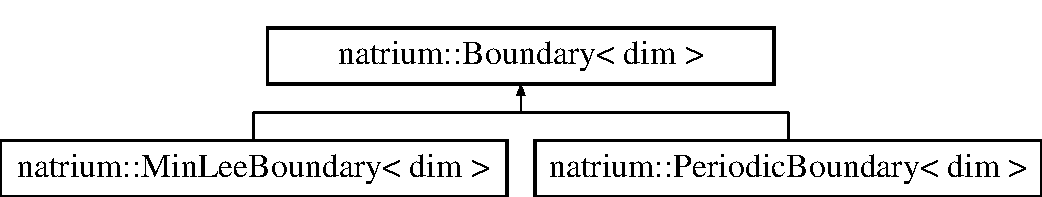
\includegraphics[height=2.000000cm]{classnatrium_1_1Boundary}
\end{center}
\end{figure}
\subsection*{Public Member Functions}
\begin{DoxyCompactItemize}
\item 
\hypertarget{classnatrium_1_1Boundary_a987978143b16ef0bbadd2b465dc1882d}{\hyperlink{classnatrium_1_1Boundary_a987978143b16ef0bbadd2b465dc1882d}{Boundary} ()}\label{classnatrium_1_1Boundary_a987978143b16ef0bbadd2b465dc1882d}

\begin{DoxyCompactList}\small\item\em constructor \end{DoxyCompactList}\item 
\hypertarget{classnatrium_1_1Boundary_a63e8fb8ec44288b9145f819b515ae6d9}{virtual \hyperlink{classnatrium_1_1Boundary_a63e8fb8ec44288b9145f819b515ae6d9}{$\sim$\-Boundary} ()}\label{classnatrium_1_1Boundary_a63e8fb8ec44288b9145f819b515ae6d9}

\begin{DoxyCompactList}\small\item\em destructor \end{DoxyCompactList}\item 
\hypertarget{classnatrium_1_1Boundary_acb651f4148b4e00f08258e1321c43235}{virtual bool \hyperlink{classnatrium_1_1Boundary_acb651f4148b4e00f08258e1321c43235}{is\-Periodic} () const }\label{classnatrium_1_1Boundary_acb651f4148b4e00f08258e1321c43235}

\begin{DoxyCompactList}\small\item\em is the boundary a periodic boundary ? \end{DoxyCompactList}\end{DoxyCompactItemize}


\subsection{Detailed Description}
\subsubsection*{template$<$size\-\_\-t dim$>$class natrium\-::\-Boundary$<$ dim $>$}

Abstract class for the description of boundaries. Base class of \hyperlink{classnatrium_1_1PeriodicBoundary}{Periodic\-Boundary}, Inflow\-Boundary, etc. 


\begin{DoxyTemplParams}{Template Parameters}
{\em dim} & The dimension of the boundary is the dimension of the domain -\/1 ( e.\-g. 2-\/dim meshes have 1-\/dim boundary) \\
\hline
\end{DoxyTemplParams}


The documentation for this class was generated from the following file\-:\begin{DoxyCompactItemize}
\item 
/home/kraemer/eclipse\-\_\-workspace/\-N\-A\-Triu\-M/src/natrium/problemdescription/\hyperlink{Boundary_8h}{Boundary.\-h}\end{DoxyCompactItemize}

\hypertarget{classnatrium_1_1BoundaryCollection}{
\section{natrium::BoundaryCollection$<$ dim $>$ Class Template Reference}
\label{classnatrium_1_1BoundaryCollection}\index{natrium::BoundaryCollection@{natrium::BoundaryCollection}}
}


The \hyperlink{classnatrium_1_1BoundaryCollection}{BoundaryCollection} class defines all boundaries of a flow domain. Internally, the boundaries are stored in two different std::map, one for the periodic boundaries and one for the non-\/periodic ones. Its keys are the boundary indicators (for periodic boundaries: the first boundary indicator).  


{\ttfamily \#include $<$BoundaryCollection.h$>$}\subsection*{Public Types}
\begin{DoxyCompactItemize}
\item 
\hypertarget{classnatrium_1_1BoundaryCollection_a8f113a1640c2f088c86f24cf9ddf4be6}{
typedef std::map$<$ size\_\-t, shared\_\-ptr$<$ \hyperlink{classnatrium_1_1Boundary}{Boundary}$<$ dim $>$ $>$ $>$::iterator {\bfseries Iterator}}
\label{classnatrium_1_1BoundaryCollection_a8f113a1640c2f088c86f24cf9ddf4be6}

\item 
\hypertarget{classnatrium_1_1BoundaryCollection_a7b7a9bd9ff95ffe3cfdec0d6efcbdf81}{
typedef std::map$<$ size\_\-t, shared\_\-ptr$<$ \hyperlink{classnatrium_1_1Boundary}{Boundary}$<$ dim $>$ $>$ $>$::const\_\-iterator {\bfseries ConstIterator}}
\label{classnatrium_1_1BoundaryCollection_a7b7a9bd9ff95ffe3cfdec0d6efcbdf81}

\item 
\hypertarget{classnatrium_1_1BoundaryCollection_aba4f994dd4290e55b888ac51800bbe9e}{
typedef std::map$<$ size\_\-t, shared\_\-ptr$<$ \hyperlink{classnatrium_1_1MinLeeBoundary}{MinLeeBoundary}$<$ dim $>$ $>$ $>$::iterator {\bfseries MinLeeIterator}}
\label{classnatrium_1_1BoundaryCollection_aba4f994dd4290e55b888ac51800bbe9e}

\item 
\hypertarget{classnatrium_1_1BoundaryCollection_a5248927752b4e9ac21dfc1a3e010e79d}{
typedef std::map$<$ size\_\-t, shared\_\-ptr$<$ \hyperlink{classnatrium_1_1MinLeeBoundary}{MinLeeBoundary}$<$ dim $>$ $>$ $>$::const\_\-iterator {\bfseries ConstMinLeeIterator}}
\label{classnatrium_1_1BoundaryCollection_a5248927752b4e9ac21dfc1a3e010e79d}

\item 
\hypertarget{classnatrium_1_1BoundaryCollection_a7cf1943ddd37e2d31d41483365de04a2}{
typedef std::map$<$ size\_\-t, shared\_\-ptr$<$ \hyperlink{classnatrium_1_1PeriodicBoundary}{PeriodicBoundary}$<$ dim $>$ $>$ $>$::iterator {\bfseries PeriodicIterator}}
\label{classnatrium_1_1BoundaryCollection_a7cf1943ddd37e2d31d41483365de04a2}

\item 
\hypertarget{classnatrium_1_1BoundaryCollection_a132c389d4a4c65e2fad4c428c7183f8b}{
typedef std::map$<$ size\_\-t, shared\_\-ptr$<$ \hyperlink{classnatrium_1_1PeriodicBoundary}{PeriodicBoundary}$<$ dim $>$ $>$ $>$::const\_\-iterator {\bfseries ConstPeriodicIterator}}
\label{classnatrium_1_1BoundaryCollection_a132c389d4a4c65e2fad4c428c7183f8b}

\end{DoxyCompactItemize}
\subsection*{Public Member Functions}
\begin{DoxyCompactItemize}
\item 
void \hyperlink{classnatrium_1_1BoundaryCollection_a60d5efd5fa9bf2107705ee1a38508dd4}{addBoundary} (shared\_\-ptr$<$ \hyperlink{classnatrium_1_1PeriodicBoundary}{PeriodicBoundary}$<$ dim $>$ $>$ boundary)
\begin{DoxyCompactList}\small\item\em Add a boundary to the flow definition. This definition of addBoundary applies to periodic boundaries. As periodic boundaries have two boundary indicators, they are added twice to the boundary map. Internally, they are additionally added to the vector periodicBoundaries, which can be accessed separate from non-\/periodic boundaries. \item\end{DoxyCompactList}\item 
void \hyperlink{classnatrium_1_1BoundaryCollection_ac8ad257c880937c59baad2d646392d7d}{addBoundary} (shared\_\-ptr$<$ \hyperlink{classnatrium_1_1MinLeeBoundary}{MinLeeBoundary}$<$ dim $>$ $>$ boundary)
\begin{DoxyCompactList}\small\item\em Add a boundary to the flow definition. \item\end{DoxyCompactList}\item 
const shared\_\-ptr$<$ \hyperlink{classnatrium_1_1Boundary}{Boundary}$<$ dim $>$ $>$ \& \hyperlink{classnatrium_1_1BoundaryCollection_adacc8205b74bdc7344161e73f1acadca}{getBoundary} (size\_\-t boundaryIndicator) const 
\begin{DoxyCompactList}\small\item\em get a specific boundary \item\end{DoxyCompactList}\item 
const shared\_\-ptr$<$ \hyperlink{classnatrium_1_1PeriodicBoundary}{PeriodicBoundary}$<$ dim $>$ $>$ \& \hyperlink{classnatrium_1_1BoundaryCollection_ac3a84114a57f0e321a24eaa743a141f3}{getPeriodicBoundary} (size\_\-t boundaryIndicator) const 
\begin{DoxyCompactList}\small\item\em get a specific periodic boundary \item\end{DoxyCompactList}\item 
const shared\_\-ptr$<$ \hyperlink{classnatrium_1_1MinLeeBoundary}{MinLeeBoundary}$<$ dim $>$ $>$ \& \hyperlink{classnatrium_1_1BoundaryCollection_aea35fe9645fc3521da83ae83ef84967b}{getMinLeeBoundary} (size\_\-t boundaryIndicator) const 
\begin{DoxyCompactList}\small\item\em get a specific MinLee boundary \item\end{DoxyCompactList}\item 
\hypertarget{classnatrium_1_1BoundaryCollection_aec4a9de4aaccaa7a49e5308bf9812c66}{
bool \hyperlink{classnatrium_1_1BoundaryCollection_aec4a9de4aaccaa7a49e5308bf9812c66}{isPeriodic} (size\_\-t boundaryIndicator) const }
\label{classnatrium_1_1BoundaryCollection_aec4a9de4aaccaa7a49e5308bf9812c66}

\begin{DoxyCompactList}\small\item\em test if the boundary with the given boundary indicator is periodic \item\end{DoxyCompactList}\item 
\hypertarget{classnatrium_1_1BoundaryCollection_ad9dbba7ffccaa31ee79cace73197148e}{
size\_\-t {\bfseries numberOfBoundaries} () const }
\label{classnatrium_1_1BoundaryCollection_ad9dbba7ffccaa31ee79cace73197148e}

\item 
\hypertarget{classnatrium_1_1BoundaryCollection_a62004be7508761795d894ed7ca7e4eb8}{
size\_\-t {\bfseries numberOfPeriodicBoundaries} () const }
\label{classnatrium_1_1BoundaryCollection_a62004be7508761795d894ed7ca7e4eb8}

\item 
\hypertarget{classnatrium_1_1BoundaryCollection_ab1454365bef1b79a2bd38148f8037be6}{
const std::map$<$ size\_\-t, shared\_\-ptr$<$ \hyperlink{classnatrium_1_1Boundary}{Boundary}$<$ dim $>$ $>$ $>$ \& {\bfseries getBoundaries} () const }
\label{classnatrium_1_1BoundaryCollection_ab1454365bef1b79a2bd38148f8037be6}

\item 
\hypertarget{classnatrium_1_1BoundaryCollection_a3f72a07f410649d80f3077046521b551}{
const std::map$<$ size\_\-t, shared\_\-ptr$<$ \hyperlink{classnatrium_1_1PeriodicBoundary}{PeriodicBoundary}$<$ dim $>$ $>$ $>$ \& {\bfseries getPeriodicBoundaries} () const }
\label{classnatrium_1_1BoundaryCollection_a3f72a07f410649d80f3077046521b551}

\item 
\hypertarget{classnatrium_1_1BoundaryCollection_a9a56438d4dfcfafe5842882fe34bbe0e}{
const std::map$<$ size\_\-t, shared\_\-ptr$<$ \hyperlink{classnatrium_1_1MinLeeBoundary}{MinLeeBoundary}$<$ dim $>$ $>$ $>$ \& {\bfseries getMinLeeBoundaries} () const }
\label{classnatrium_1_1BoundaryCollection_a9a56438d4dfcfafe5842882fe34bbe0e}

\end{DoxyCompactItemize}


\subsection{Detailed Description}
\subsubsection*{template$<$size\_\-t dim$>$ class natrium::BoundaryCollection$<$ dim $>$}

The \hyperlink{classnatrium_1_1BoundaryCollection}{BoundaryCollection} class defines all boundaries of a flow domain. Internally, the boundaries are stored in two different std::map, one for the periodic boundaries and one for the non-\/periodic ones. Its keys are the boundary indicators (for periodic boundaries: the first boundary indicator). 

\subsection{Member Function Documentation}
\hypertarget{classnatrium_1_1BoundaryCollection_ac8ad257c880937c59baad2d646392d7d}{
\index{natrium::BoundaryCollection@{natrium::BoundaryCollection}!addBoundary@{addBoundary}}
\index{addBoundary@{addBoundary}!natrium::BoundaryCollection@{natrium::BoundaryCollection}}
\subsubsection[{addBoundary}]{\setlength{\rightskip}{0pt plus 5cm}template$<$size\_\-t dim$>$ void {\bf natrium::BoundaryCollection}$<$ dim $>$::addBoundary (shared\_\-ptr$<$ {\bf MinLeeBoundary}$<$ dim $>$ $>$ {\em boundary})\hspace{0.3cm}{\ttfamily  \mbox{[}inline\mbox{]}}}}
\label{classnatrium_1_1BoundaryCollection_ac8ad257c880937c59baad2d646392d7d}


Add a boundary to the flow definition. 
\begin{DoxyParams}{Parameters}
\item[{\em boundary}]a periodic boundary \end{DoxyParams}

\begin{DoxyExceptions}{Exceptions}
\item[{\em BoundaryCollectionError,e.g.}]if boundary indicators are not unique \end{DoxyExceptions}
\hypertarget{classnatrium_1_1BoundaryCollection_a60d5efd5fa9bf2107705ee1a38508dd4}{
\index{natrium::BoundaryCollection@{natrium::BoundaryCollection}!addBoundary@{addBoundary}}
\index{addBoundary@{addBoundary}!natrium::BoundaryCollection@{natrium::BoundaryCollection}}
\subsubsection[{addBoundary}]{\setlength{\rightskip}{0pt plus 5cm}template$<$size\_\-t dim$>$ void {\bf natrium::BoundaryCollection}$<$ dim $>$::addBoundary (shared\_\-ptr$<$ {\bf PeriodicBoundary}$<$ dim $>$ $>$ {\em boundary})\hspace{0.3cm}{\ttfamily  \mbox{[}inline\mbox{]}}}}
\label{classnatrium_1_1BoundaryCollection_a60d5efd5fa9bf2107705ee1a38508dd4}


Add a boundary to the flow definition. This definition of addBoundary applies to periodic boundaries. As periodic boundaries have two boundary indicators, they are added twice to the boundary map. Internally, they are additionally added to the vector periodicBoundaries, which can be accessed separate from non-\/periodic boundaries. 
\begin{DoxyParams}{Parameters}
\item[{\em boundary}]a periodic boundary \end{DoxyParams}

\begin{DoxyExceptions}{Exceptions}
\item[{\em BoundaryCollectionError,e.g.}]if boundary indicators are not unique \end{DoxyExceptions}
\hypertarget{classnatrium_1_1BoundaryCollection_adacc8205b74bdc7344161e73f1acadca}{
\index{natrium::BoundaryCollection@{natrium::BoundaryCollection}!getBoundary@{getBoundary}}
\index{getBoundary@{getBoundary}!natrium::BoundaryCollection@{natrium::BoundaryCollection}}
\subsubsection[{getBoundary}]{\setlength{\rightskip}{0pt plus 5cm}template$<$size\_\-t dim$>$ const shared\_\-ptr$<${\bf Boundary}$<$dim$>$ $>$\& {\bf natrium::BoundaryCollection}$<$ dim $>$::getBoundary (size\_\-t {\em boundaryIndicator}) const\hspace{0.3cm}{\ttfamily  \mbox{[}inline\mbox{]}}}}
\label{classnatrium_1_1BoundaryCollection_adacc8205b74bdc7344161e73f1acadca}


get a specific boundary 
\begin{DoxyExceptions}{Exceptions}
\item[{\em BoundaryCollectionError,if}]the specified boundary indicator does not exist \end{DoxyExceptions}
\hypertarget{classnatrium_1_1BoundaryCollection_aea35fe9645fc3521da83ae83ef84967b}{
\index{natrium::BoundaryCollection@{natrium::BoundaryCollection}!getMinLeeBoundary@{getMinLeeBoundary}}
\index{getMinLeeBoundary@{getMinLeeBoundary}!natrium::BoundaryCollection@{natrium::BoundaryCollection}}
\subsubsection[{getMinLeeBoundary}]{\setlength{\rightskip}{0pt plus 5cm}template$<$size\_\-t dim$>$ const shared\_\-ptr$<${\bf MinLeeBoundary}$<$dim$>$ $>$\& {\bf natrium::BoundaryCollection}$<$ dim $>$::getMinLeeBoundary (size\_\-t {\em boundaryIndicator}) const\hspace{0.3cm}{\ttfamily  \mbox{[}inline\mbox{]}}}}
\label{classnatrium_1_1BoundaryCollection_aea35fe9645fc3521da83ae83ef84967b}


get a specific MinLee boundary 
\begin{DoxyExceptions}{Exceptions}
\item[{\em BoundaryCollectionError,if}]the specified boundary indicator does not exist \end{DoxyExceptions}
\hypertarget{classnatrium_1_1BoundaryCollection_ac3a84114a57f0e321a24eaa743a141f3}{
\index{natrium::BoundaryCollection@{natrium::BoundaryCollection}!getPeriodicBoundary@{getPeriodicBoundary}}
\index{getPeriodicBoundary@{getPeriodicBoundary}!natrium::BoundaryCollection@{natrium::BoundaryCollection}}
\subsubsection[{getPeriodicBoundary}]{\setlength{\rightskip}{0pt plus 5cm}template$<$size\_\-t dim$>$ const shared\_\-ptr$<${\bf PeriodicBoundary}$<$dim$>$ $>$\& {\bf natrium::BoundaryCollection}$<$ dim $>$::getPeriodicBoundary (size\_\-t {\em boundaryIndicator}) const\hspace{0.3cm}{\ttfamily  \mbox{[}inline\mbox{]}}}}
\label{classnatrium_1_1BoundaryCollection_ac3a84114a57f0e321a24eaa743a141f3}


get a specific periodic boundary 
\begin{DoxyExceptions}{Exceptions}
\item[{\em BoundaryCollectionError,if}]the specified boundary indicator does not exist \end{DoxyExceptions}


The documentation for this class was generated from the following file:\begin{DoxyCompactItemize}
\item 
/mnt/fdrive/akraem3m/workspace/NATriuM/src/library/natrium/problemdescription/BoundaryCollection.h\end{DoxyCompactItemize}

\hypertarget{classnatrium_1_1BoundaryCollectionError}{\section{natrium\-:\-:Boundary\-Collection\-Error Class Reference}
\label{classnatrium_1_1BoundaryCollectionError}\index{natrium\-::\-Boundary\-Collection\-Error@{natrium\-::\-Boundary\-Collection\-Error}}
}


\hyperlink{classnatrium_1_1Boundary}{Boundary} errors (e.\-g. duplicate boundary indicators)  




{\ttfamily \#include $<$Boundary\-Collection.\-h$>$}

Inheritance diagram for natrium\-:\-:Boundary\-Collection\-Error\-:\begin{figure}[H]
\begin{center}
\leavevmode
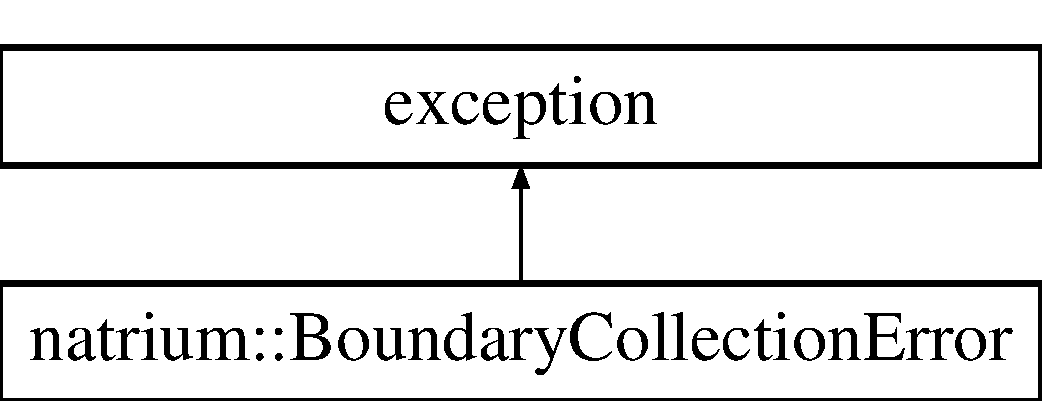
\includegraphics[height=2.000000cm]{classnatrium_1_1BoundaryCollectionError}
\end{center}
\end{figure}
\subsection*{Public Member Functions}
\begin{DoxyCompactItemize}
\item 
\hypertarget{classnatrium_1_1BoundaryCollectionError_a4eb02d034a4a61142ca0d93a633babdd}{{\bfseries Boundary\-Collection\-Error} (const std\-::string \&message)}\label{classnatrium_1_1BoundaryCollectionError_a4eb02d034a4a61142ca0d93a633babdd}

\item 
\hypertarget{classnatrium_1_1BoundaryCollectionError_ac80dc49f07da4dc6353b7d62d28a42fa}{virtual const char $\ast$ {\bfseries what} () const   throw ()}\label{classnatrium_1_1BoundaryCollectionError_ac80dc49f07da4dc6353b7d62d28a42fa}

\end{DoxyCompactItemize}


\subsection{Detailed Description}
\hyperlink{classnatrium_1_1Boundary}{Boundary} errors (e.\-g. duplicate boundary indicators) 

The documentation for this class was generated from the following file\-:\begin{DoxyCompactItemize}
\item 
/home/kraemer/eclipse\-\_\-workspace/\-N\-A\-Triu\-M/src/natrium/problemdescription/Boundary\-Collection.\-h\end{DoxyCompactItemize}

\hypertarget{classnatrium_1_1BoundaryDensity}{\section{natrium\-:\-:Boundary\-Density Class Reference}
\label{classnatrium_1_1BoundaryDensity}\index{natrium\-::\-Boundary\-Density@{natrium\-::\-Boundary\-Density}}
}
Inheritance diagram for natrium\-:\-:Boundary\-Density\-:\begin{figure}[H]
\begin{center}
\leavevmode
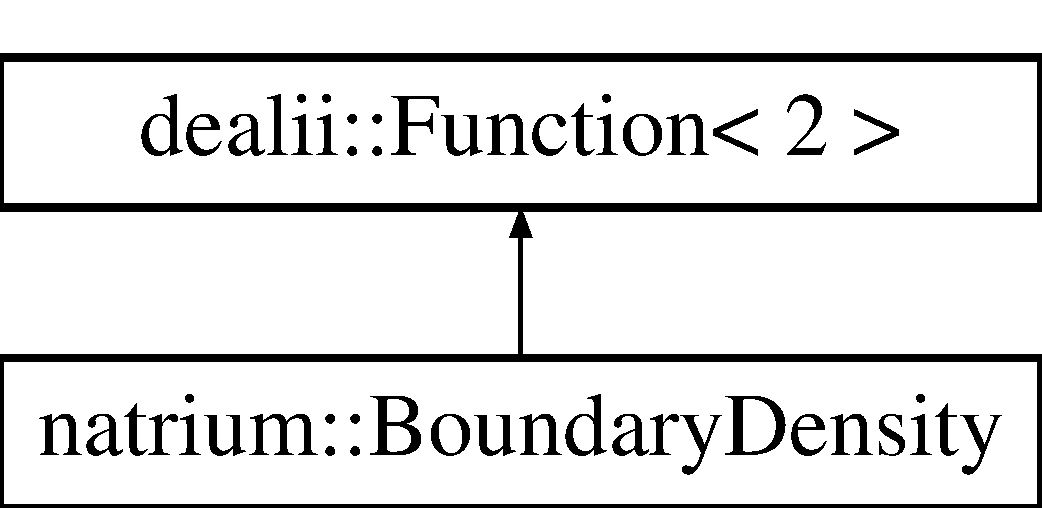
\includegraphics[height=2.000000cm]{classnatrium_1_1BoundaryDensity}
\end{center}
\end{figure}
\subsection*{Public Member Functions}
\begin{DoxyCompactItemize}
\item 
\hypertarget{classnatrium_1_1BoundaryDensity_aea4a63e9b0ef8a965b61d3a9bfcd076e}{virtual double {\bfseries value} (const dealii\-::\-Point$<$ 2 $>$ \&p, const unsigned int component=0) const }\label{classnatrium_1_1BoundaryDensity_aea4a63e9b0ef8a965b61d3a9bfcd076e}

\end{DoxyCompactItemize}


The documentation for this class was generated from the following file\-:\begin{DoxyCompactItemize}
\item 
/home/kraemer/eclipse\-\_\-workspace/\-N\-A\-Triu\-M/src/natrium/problemdescription/\hyperlink{MinLeeBoundary_8h}{Min\-Lee\-Boundary.\-h}\end{DoxyCompactItemize}

\hypertarget{classnatrium_1_1BoundaryTestDensity}{
\section{natrium::BoundaryTestDensity Class Reference}
\label{classnatrium_1_1BoundaryTestDensity}\index{natrium::BoundaryTestDensity@{natrium::BoundaryTestDensity}}
}
\subsection*{Public Member Functions}
\begin{DoxyCompactItemize}
\item 
\hypertarget{classnatrium_1_1BoundaryTestDensity_af485f34989fac863e20d1827f379cfa6}{
virtual double {\bfseries value} (const dealii::Point$<$ 2 $>$ \&, const unsigned int) const }
\label{classnatrium_1_1BoundaryTestDensity_af485f34989fac863e20d1827f379cfa6}

\end{DoxyCompactItemize}


The documentation for this class was generated from the following file:\begin{DoxyCompactItemize}
\item 
/mnt/fdrive/akraem3m/workspace/NATriuM/src/test/boundaries/DirichletBoundaryRhoU2D\_\-test.cpp\end{DoxyCompactItemize}

\hypertarget{classnatrium_1_1BoundaryTestVelocity}{
\section{natrium::BoundaryTestVelocity Class Reference}
\label{classnatrium_1_1BoundaryTestVelocity}\index{natrium::BoundaryTestVelocity@{natrium::BoundaryTestVelocity}}
}
\subsection*{Public Member Functions}
\begin{DoxyCompactItemize}
\item 
\hypertarget{classnatrium_1_1BoundaryTestVelocity_a79517bd2413986c38f4e944faea57a48}{
virtual void {\bfseries vector\_\-value} (const dealii::Point$<$ 2 $>$ \&, dealii::Vector$<$ double $>$ \&values) const }
\label{classnatrium_1_1BoundaryTestVelocity_a79517bd2413986c38f4e944faea57a48}

\end{DoxyCompactItemize}


The documentation for this class was generated from the following file:\begin{DoxyCompactItemize}
\item 
/mnt/fdrive/akraem3m/workspace/NATriuM/src/test/problemdescription/DirichletBoundaryRhoU2D\_\-test.cpp\end{DoxyCompactItemize}

\hypertarget{classnatrium_1_1BoundaryVelocity}{\section{natrium\-:\-:Boundary\-Velocity Class Reference}
\label{classnatrium_1_1BoundaryVelocity}\index{natrium\-::\-Boundary\-Velocity@{natrium\-::\-Boundary\-Velocity}}
}
Inheritance diagram for natrium\-:\-:Boundary\-Velocity\-:\begin{figure}[H]
\begin{center}
\leavevmode
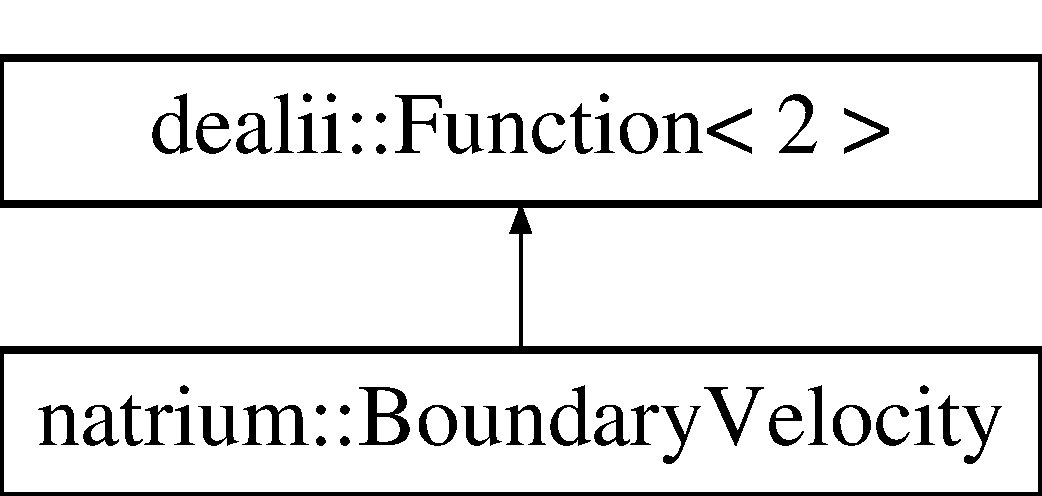
\includegraphics[height=2.000000cm]{classnatrium_1_1BoundaryVelocity}
\end{center}
\end{figure}
\subsection*{Public Member Functions}
\begin{DoxyCompactItemize}
\item 
\hypertarget{classnatrium_1_1BoundaryVelocity_a2deefe9da743338b45f2382ecc50f942}{{\bfseries Boundary\-Velocity} (const dealii\-::\-Vector$<$ double $>$ \&velocity)}\label{classnatrium_1_1BoundaryVelocity_a2deefe9da743338b45f2382ecc50f942}

\item 
\hypertarget{classnatrium_1_1BoundaryVelocity_a468a9411f08b9a6c6f484e096f7d57a1}{virtual void {\bfseries vector\-\_\-value} (const dealii\-::\-Point$<$ 2 $>$ \&p, dealii\-::\-Vector$<$ double $>$ \&values) const }\label{classnatrium_1_1BoundaryVelocity_a468a9411f08b9a6c6f484e096f7d57a1}

\end{DoxyCompactItemize}


The documentation for this class was generated from the following file\-:\begin{DoxyCompactItemize}
\item 
/home/kraemer/eclipse\-\_\-workspace/\-N\-A\-Triu\-M/src/natrium/problemdescription/\hyperlink{MinLeeBoundary_8h}{Min\-Lee\-Boundary.\-h}\end{DoxyCompactItemize}

\hypertarget{classnatrium_1_1CFDSolver}{
\section{natrium::CFDSolver$<$ dim $>$ Class Template Reference}
\label{classnatrium_1_1CFDSolver}\index{natrium::CFDSolver@{natrium::CFDSolver}}
}


The central class for the CFD simulation based on the DBE.  


{\ttfamily \#include $<$CFDSolver.h$>$}Inheritance diagram for natrium::CFDSolver$<$ dim $>$::\begin{figure}[H]
\begin{center}
\leavevmode
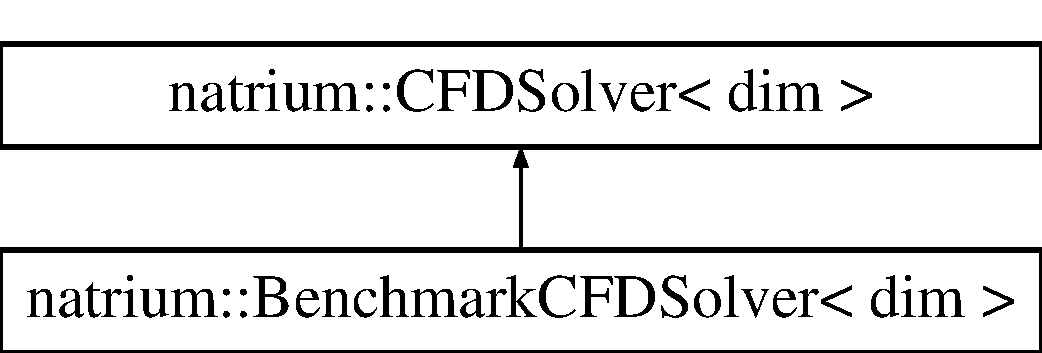
\includegraphics[height=2cm]{classnatrium_1_1CFDSolver}
\end{center}
\end{figure}
\subsection*{Public Member Functions}
\begin{DoxyCompactItemize}
\item 
\hyperlink{classnatrium_1_1CFDSolver_a9d0e65b8a404ac3eaf80aee6c81945dc}{CFDSolver} (shared\_\-ptr$<$ \hyperlink{classnatrium_1_1SolverConfiguration}{SolverConfiguration} $>$ configuration, shared\_\-ptr$<$ \hyperlink{classnatrium_1_1ProblemDescription}{ProblemDescription}$<$ dim $>$ $>$ problemDescription)
\item 
\hypertarget{classnatrium_1_1CFDSolver_a7ca9bd709255ac87b34f869c984b913b}{
virtual \hyperlink{classnatrium_1_1CFDSolver_a7ca9bd709255ac87b34f869c984b913b}{$\sim$CFDSolver} ()}
\label{classnatrium_1_1CFDSolver_a7ca9bd709255ac87b34f869c984b913b}

\begin{DoxyCompactList}\small\item\em destructor \item\end{DoxyCompactList}\item 
\hypertarget{classnatrium_1_1CFDSolver_abe627b0bbde0635abb30b9bea4c72dc1}{
void \hyperlink{classnatrium_1_1CFDSolver_abe627b0bbde0635abb30b9bea4c72dc1}{initializeDistributions} ()}
\label{classnatrium_1_1CFDSolver_abe627b0bbde0635abb30b9bea4c72dc1}

\begin{DoxyCompactList}\small\item\em initialize distribution functions \item\end{DoxyCompactList}\item 
\hypertarget{classnatrium_1_1CFDSolver_ac32a318e504b31195eb61c2cdc2659fe}{
void \hyperlink{classnatrium_1_1CFDSolver_ac32a318e504b31195eb61c2cdc2659fe}{stream} ()}
\label{classnatrium_1_1CFDSolver_ac32a318e504b31195eb61c2cdc2659fe}

\begin{DoxyCompactList}\small\item\em Advection in all directions. \item\end{DoxyCompactList}\item 
\hypertarget{classnatrium_1_1CFDSolver_ac9bec7d0c4bcd5e02c5213ec09438c02}{
void \hyperlink{classnatrium_1_1CFDSolver_ac9bec7d0c4bcd5e02c5213ec09438c02}{collide} ()}
\label{classnatrium_1_1CFDSolver_ac9bec7d0c4bcd5e02c5213ec09438c02}

\begin{DoxyCompactList}\small\item\em Low-\/level collide function. \item\end{DoxyCompactList}\item 
\hypertarget{classnatrium_1_1CFDSolver_a604212a1f6cd2549b8f60ab26b14de00}{
void \hyperlink{classnatrium_1_1CFDSolver_a604212a1f6cd2549b8f60ab26b14de00}{reassemble} ()}
\label{classnatrium_1_1CFDSolver_a604212a1f6cd2549b8f60ab26b14de00}

\begin{DoxyCompactList}\small\item\em reassembly of all matrices \item\end{DoxyCompactList}\item 
\hypertarget{classnatrium_1_1CFDSolver_a11f503bc3f3c306b240874c74a38025b}{
void \hyperlink{classnatrium_1_1CFDSolver_a11f503bc3f3c306b240874c74a38025b}{run} ()}
\label{classnatrium_1_1CFDSolver_a11f503bc3f3c306b240874c74a38025b}

\begin{DoxyCompactList}\small\item\em run CFD solver \item\end{DoxyCompactList}\item 
\hypertarget{classnatrium_1_1CFDSolver_a9a144e7e757e1b1c26f32b712b17c70e}{
bool \hyperlink{classnatrium_1_1CFDSolver_a9a144e7e757e1b1c26f32b712b17c70e}{stopConditionMet} ()}
\label{classnatrium_1_1CFDSolver_a9a144e7e757e1b1c26f32b712b17c70e}

\begin{DoxyCompactList}\small\item\em test for stop conditions \item\end{DoxyCompactList}\item 
void \hyperlink{classnatrium_1_1CFDSolver_a36146c0f8a6c5abd0ebec4c49f2a4e6d}{applyInitialDensities} (distributed\_\-vector \&initialDensities, const map$<$ dealii::types::global\_\-dof\_\-index, dealii::Point$<$ dim $>$ $>$ \&supportPoints) const 
\begin{DoxyCompactList}\small\item\em set initial densities \item\end{DoxyCompactList}\item 
void \hyperlink{classnatrium_1_1CFDSolver_afd82bfa5e1e613ef99b9b870cb73db0e}{applyInitialVelocities} (vector$<$ distributed\_\-vector $>$ \&initialVelocities, const map$<$ dealii::types::global\_\-dof\_\-index, dealii::Point$<$ dim $>$ $>$ \&supportPoints) const 
\begin{DoxyCompactList}\small\item\em set initial velocities \item\end{DoxyCompactList}\item 
virtual void \hyperlink{classnatrium_1_1CFDSolver_abf6804f132885502b61877fc1f9ca4a2}{output} (size\_\-t iteration)
\begin{DoxyCompactList}\small\item\em create output data and write to file \item\end{DoxyCompactList}\item 
\hypertarget{classnatrium_1_1CFDSolver_a9c3f844b4c6b670aac83bc3ad5519fad}{
bool {\bfseries hasGeometryChanged} ()}
\label{classnatrium_1_1CFDSolver_a9c3f844b4c6b670aac83bc3ad5519fad}

\item 
\hypertarget{classnatrium_1_1CFDSolver_adf0b4e4da292bcb195d926d3174ba2a9}{
const distributed\_\-vector \& {\bfseries getDensity} () const }
\label{classnatrium_1_1CFDSolver_adf0b4e4da292bcb195d926d3174ba2a9}

\item 
\hypertarget{classnatrium_1_1CFDSolver_a963e069873d88d130b0fe3f7f77c3d83}{
const \hyperlink{classnatrium_1_1DistributionFunctions}{DistributionFunctions} \& {\bfseries getF} () const }
\label{classnatrium_1_1CFDSolver_a963e069873d88d130b0fe3f7f77c3d83}

\item 
\hypertarget{classnatrium_1_1CFDSolver_a0e5ec3dc278216d5827410b7db82af59}{
const vector$<$ distributed\_\-vector $>$ \& {\bfseries getVelocity} () const }
\label{classnatrium_1_1CFDSolver_a0e5ec3dc278216d5827410b7db82af59}

\item 
\hypertarget{classnatrium_1_1CFDSolver_a1aea207c81089c2e46092489557bb139}{
const shared\_\-ptr$<$ \hyperlink{classnatrium_1_1AdvectionOperator}{AdvectionOperator}$<$ dim $>$ $>$ \& {\bfseries getAdvectionOperator} () const }
\label{classnatrium_1_1CFDSolver_a1aea207c81089c2e46092489557bb139}

\item 
\hypertarget{classnatrium_1_1CFDSolver_a2006f7bbbf2336789a5cd74d329c2e60}{
const shared\_\-ptr$<$ \hyperlink{classnatrium_1_1Stencil}{Stencil} $>$ \& {\bfseries getStencil} () const }
\label{classnatrium_1_1CFDSolver_a2006f7bbbf2336789a5cd74d329c2e60}

\item 
\hypertarget{classnatrium_1_1CFDSolver_abb4b632b524bd68afcdff7d54c2d3d97}{
const shared\_\-ptr$<$ \hyperlink{classnatrium_1_1CollisionModel}{CollisionModel} $>$ \& {\bfseries getCollisionModel} () const }
\label{classnatrium_1_1CFDSolver_abb4b632b524bd68afcdff7d54c2d3d97}

\item 
\hypertarget{classnatrium_1_1CFDSolver_a413691491ac82f384a03293be2294de5}{
const shared\_\-ptr$<$ \hyperlink{classnatrium_1_1SolverConfiguration}{SolverConfiguration} $>$ \& {\bfseries getConfiguration} () const }
\label{classnatrium_1_1CFDSolver_a413691491ac82f384a03293be2294de5}

\item 
\hypertarget{classnatrium_1_1CFDSolver_a8b1131e8fd6b022bea5ddce72469c289}{
const shared\_\-ptr$<$ \hyperlink{classnatrium_1_1ProblemDescription}{ProblemDescription}$<$ dim $>$ $>$ \& {\bfseries getProblemDescription} () const }
\label{classnatrium_1_1CFDSolver_a8b1131e8fd6b022bea5ddce72469c289}

\item 
\hypertarget{classnatrium_1_1CFDSolver_af1b1ca6771029003bc9bac7cfe0b4d3c}{
const shared\_\-ptr$<$ \hyperlink{classnatrium_1_1TimeIntegrator}{TimeIntegrator}$<$ distributed\_\-vector, distributed\_\-sparse\_\-matrix $>$ $>$ \& {\bfseries getTimeIntegrator} () const }
\label{classnatrium_1_1CFDSolver_af1b1ca6771029003bc9bac7cfe0b4d3c}

\item 
\hypertarget{classnatrium_1_1CFDSolver_a74d459ef4f43d42e04ceb2178bb006f4}{
size\_\-t {\bfseries getNumberOfDoFs} () const }
\label{classnatrium_1_1CFDSolver_a74d459ef4f43d42e04ceb2178bb006f4}

\item 
\hypertarget{classnatrium_1_1CFDSolver_ae9c44bb0f33e2c73ee96fbe100061842}{
double {\bfseries getMaxVelocityNorm} () const }
\label{classnatrium_1_1CFDSolver_ae9c44bb0f33e2c73ee96fbe100061842}

\item 
\hypertarget{classnatrium_1_1CFDSolver_ade641431988a82cb47d88a9d600e1c92}{
double {\bfseries getMaxDensityDeviationFrom} (double referenceDensity) const }
\label{classnatrium_1_1CFDSolver_ade641431988a82cb47d88a9d600e1c92}

\item 
\hypertarget{classnatrium_1_1CFDSolver_a33c4bfd63b8d457a5bc15f0c0da02c38}{
size\_\-t {\bfseries getIterationStart} () const }
\label{classnatrium_1_1CFDSolver_a33c4bfd63b8d457a5bc15f0c0da02c38}

\item 
\hypertarget{classnatrium_1_1CFDSolver_a8e3686b16794c0040bd5cc7cf9fe98d3}{
double {\bfseries getTime} () const }
\label{classnatrium_1_1CFDSolver_a8e3686b16794c0040bd5cc7cf9fe98d3}

\item 
\hypertarget{classnatrium_1_1CFDSolver_a3c0920e02df800abcfb8f82518cab0ca}{
size\_\-t {\bfseries getIteration} () const }
\label{classnatrium_1_1CFDSolver_a3c0920e02df800abcfb8f82518cab0ca}

\item 
\hypertarget{classnatrium_1_1CFDSolver_a97546801de9259206f9611c14ce9ff1d}{
void {\bfseries setIteration} (size\_\-t iteration)}
\label{classnatrium_1_1CFDSolver_a97546801de9259206f9611c14ce9ff1d}

\item 
\hypertarget{classnatrium_1_1CFDSolver_ab40725ea85fde34033d92027d13a4b06}{
const shared\_\-ptr$<$ \hyperlink{classnatrium_1_1SolverStats}{SolverStats}$<$ dim $>$ $>$ \& {\bfseries getSolverStats} () const }
\label{classnatrium_1_1CFDSolver_ab40725ea85fde34033d92027d13a4b06}

\item 
\hypertarget{classnatrium_1_1CFDSolver_abcce31d3ba9b00e148780b6c855d189b}{
double {\bfseries getTau} () const }
\label{classnatrium_1_1CFDSolver_abcce31d3ba9b00e148780b6c855d189b}

\item 
\hypertarget{classnatrium_1_1CFDSolver_a1a508263caff799245a183989efd6680}{
double {\bfseries getResiduumDensity} () const }
\label{classnatrium_1_1CFDSolver_a1a508263caff799245a183989efd6680}

\item 
\hypertarget{classnatrium_1_1CFDSolver_a051ad2daa843e9edf9f1243b3c062686}{
double {\bfseries getResiduumVelocity} () const }
\label{classnatrium_1_1CFDSolver_a051ad2daa843e9edf9f1243b3c062686}

\end{DoxyCompactItemize}
\subsection*{Protected Member Functions}
\begin{DoxyCompactItemize}
\item 
\hypertarget{classnatrium_1_1CFDSolver_a9a2592ea549fa10427c84f0a1e380c1e}{
void \hyperlink{classnatrium_1_1CFDSolver_a9a2592ea549fa10427c84f0a1e380c1e}{saveDistributionFunctionsToFiles} (const string \&directory)}
\label{classnatrium_1_1CFDSolver_a9a2592ea549fa10427c84f0a1e380c1e}

\begin{DoxyCompactList}\small\item\em save the distribution functions to files for checkpointing \item\end{DoxyCompactList}\item 
\hypertarget{classnatrium_1_1CFDSolver_a42245d22e289d079a3b06a0c26f50050}{
void \hyperlink{classnatrium_1_1CFDSolver_a42245d22e289d079a3b06a0c26f50050}{loadDistributionFunctionsFromFiles} (const string \&directory)}
\label{classnatrium_1_1CFDSolver_a42245d22e289d079a3b06a0c26f50050}

\begin{DoxyCompactList}\small\item\em load the distribution functions from files for checkpointing \item\end{DoxyCompactList}\item 
\hypertarget{classnatrium_1_1CFDSolver_a9107b3f462bddc5b7988ec93f78797c2}{
virtual void \hyperlink{classnatrium_1_1CFDSolver_a9107b3f462bddc5b7988ec93f78797c2}{addAnalyticSolutionToOutput} (dealii::DataOut$<$ dim $>$ \&)}
\label{classnatrium_1_1CFDSolver_a9107b3f462bddc5b7988ec93f78797c2}

\begin{DoxyCompactList}\small\item\em gives the possibility for \hyperlink{classnatrium_1_1Benchmark}{Benchmark} instances to add the analytic solution to output \item\end{DoxyCompactList}\end{DoxyCompactItemize}
\subsection*{Friends}
\begin{DoxyCompactItemize}
\item 
\hypertarget{classnatrium_1_1CFDSolver_a077a2603e5a09310a68f71b538415f46}{
class {\bfseries SolverStats}}
\label{classnatrium_1_1CFDSolver_a077a2603e5a09310a68f71b538415f46}

\end{DoxyCompactItemize}


\subsection{Detailed Description}
\subsubsection*{template$<$size\_\-t dim$>$ class natrium::CFDSolver$<$ dim $>$}

The central class for the CFD simulation based on the DBE. \begin{DoxyNote}{Note}
The \hyperlink{classnatrium_1_1CFDSolver}{CFDSolver} itself is quite static but it contains interchangeable modules, e.g. for the \hyperlink{classnatrium_1_1Stencil}{Stencil} or the time integrator. By these means, a variety of different simulation methods can be covered. 
\end{DoxyNote}

\begin{DoxyTemplParams}{Template Parameters}
\item[{\em dim}]The dimension of the flow (2 or 3). \end{DoxyTemplParams}
\begin{Desc}
\item[Examples: ]\par


\hyperlink{step-0_8cpp-example}{step-\/0.cpp}.\end{Desc}


\subsection{Constructor \& Destructor Documentation}
\hypertarget{classnatrium_1_1CFDSolver_a9d0e65b8a404ac3eaf80aee6c81945dc}{
\index{natrium::CFDSolver@{natrium::CFDSolver}!CFDSolver@{CFDSolver}}
\index{CFDSolver@{CFDSolver}!natrium::CFDSolver@{natrium::CFDSolver}}
\subsubsection[{CFDSolver}]{\setlength{\rightskip}{0pt plus 5cm}template$<$size\_\-t dim$>$ {\bf natrium::CFDSolver}$<$ dim $>$::{\bf CFDSolver} (shared\_\-ptr$<$ {\bf SolverConfiguration} $>$ {\em configuration}, \/  shared\_\-ptr$<$ {\bf ProblemDescription}$<$ dim $>$ $>$ {\em problemDescription})\hspace{0.3cm}{\ttfamily  \mbox{[}inline\mbox{]}}}}
\label{classnatrium_1_1CFDSolver_a9d0e65b8a404ac3eaf80aee6c81945dc}
constructor \begin{DoxyNote}{Note}
: has to be inlined, if the template parameter is not made explicit 
\end{DoxyNote}


Create output directory

check if problem's boundary conditions are well defined

check if problem and solver configuration fit together

Build boltzmann model

Build streaming data object

Calculate relaxation parameter and build collision model

Build time integrator 

\subsection{Member Function Documentation}
\hypertarget{classnatrium_1_1CFDSolver_a36146c0f8a6c5abd0ebec4c49f2a4e6d}{
\index{natrium::CFDSolver@{natrium::CFDSolver}!applyInitialDensities@{applyInitialDensities}}
\index{applyInitialDensities@{applyInitialDensities}!natrium::CFDSolver@{natrium::CFDSolver}}
\subsubsection[{applyInitialDensities}]{\setlength{\rightskip}{0pt plus 5cm}template$<$size\_\-t dim$>$ void {\bf natrium::CFDSolver}$<$ dim $>$::applyInitialDensities (distributed\_\-vector \& {\em initialDensities}, \/  const map$<$ dealii::types::global\_\-dof\_\-index, dealii::Point$<$ dim $>$ $>$ \& {\em supportPoints}) const\hspace{0.3cm}{\ttfamily  \mbox{[}inline\mbox{]}}}}
\label{classnatrium_1_1CFDSolver_a36146c0f8a6c5abd0ebec4c49f2a4e6d}


set initial densities 
\begin{DoxyParams}{Parameters}
\item[\mbox{$\rightarrow$} {\em initialDensities}]vector of densities; to be filled \item[\mbox{$\leftarrow$} {\em supportPoints}]the coordinates associated with each degree of freedom \end{DoxyParams}
\hypertarget{classnatrium_1_1CFDSolver_afd82bfa5e1e613ef99b9b870cb73db0e}{
\index{natrium::CFDSolver@{natrium::CFDSolver}!applyInitialVelocities@{applyInitialVelocities}}
\index{applyInitialVelocities@{applyInitialVelocities}!natrium::CFDSolver@{natrium::CFDSolver}}
\subsubsection[{applyInitialVelocities}]{\setlength{\rightskip}{0pt plus 5cm}template$<$size\_\-t dim$>$ void {\bf natrium::CFDSolver}$<$ dim $>$::applyInitialVelocities (vector$<$ distributed\_\-vector $>$ \& {\em initialVelocities}, \/  const map$<$ dealii::types::global\_\-dof\_\-index, dealii::Point$<$ dim $>$ $>$ \& {\em supportPoints}) const\hspace{0.3cm}{\ttfamily  \mbox{[}inline\mbox{]}}}}
\label{classnatrium_1_1CFDSolver_afd82bfa5e1e613ef99b9b870cb73db0e}


set initial velocities 
\begin{DoxyParams}{Parameters}
\item[\mbox{$\rightarrow$} {\em initialVelocities}]vector of velocities; to be filled \item[\mbox{$\leftarrow$} {\em supportPoints}]the coordinates associated with each degree of freedom \end{DoxyParams}


Reimplemented in \hyperlink{classnatrium_1_1BenchmarkCFDSolver_a7883dcfd4469ae65ae62cad09ae5d160}{natrium::BenchmarkCFDSolver$<$ dim $>$}.\hypertarget{classnatrium_1_1CFDSolver_abf6804f132885502b61877fc1f9ca4a2}{
\index{natrium::CFDSolver@{natrium::CFDSolver}!output@{output}}
\index{output@{output}!natrium::CFDSolver@{natrium::CFDSolver}}
\subsubsection[{output}]{\setlength{\rightskip}{0pt plus 5cm}template$<$size\_\-t dim$>$ template void {\bf natrium::CFDSolver}$<$ dim $>$::output (size\_\-t {\em iteration})\hspace{0.3cm}{\ttfamily  \mbox{[}inline, virtual\mbox{]}}}}
\label{classnatrium_1_1CFDSolver_abf6804f132885502b61877fc1f9ca4a2}


create output data and write to file 

For Benchmarks: add analytic solution 

Reimplemented in \hyperlink{classnatrium_1_1BenchmarkCFDSolver_a9708132fc0cef4ae55e3453672891c81}{natrium::BenchmarkCFDSolver$<$ dim $>$}.

The documentation for this class was generated from the following files:\begin{DoxyCompactItemize}
\item 
/mnt/fdrive/akraem3m/workspace/NATriuM/src/library/natrium/solver/\hyperlink{CFDSolver_8h}{CFDSolver.h}\item 
/mnt/fdrive/akraem3m/workspace/NATriuM/src/library/natrium/solver/\hyperlink{CFDSolver_8cpp}{CFDSolver.cpp}\end{DoxyCompactItemize}

\hypertarget{classnatrium_1_1CFDSolverException}{
\section{natrium::CFDSolverException Class Reference}
\label{classnatrium_1_1CFDSolverException}\index{natrium::CFDSolverException@{natrium::CFDSolverException}}
}


Exception class for \hyperlink{classnatrium_1_1CFDSolver}{CFDSolver}.  


{\ttfamily \#include $<$CFDSolver.h$>$}Inheritance diagram for natrium::CFDSolverException::\begin{figure}[H]
\begin{center}
\leavevmode
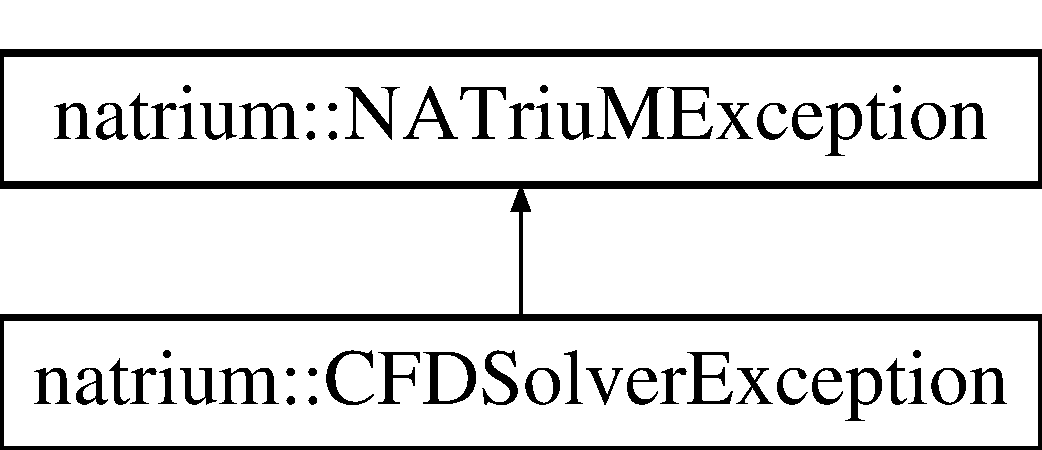
\includegraphics[height=2cm]{classnatrium_1_1CFDSolverException}
\end{center}
\end{figure}
\subsection*{Public Member Functions}
\begin{DoxyCompactItemize}
\item 
\hypertarget{classnatrium_1_1CFDSolverException_a1256570132b679d57fe046f648656051}{
{\bfseries CFDSolverException} (const char $\ast$msg)}
\label{classnatrium_1_1CFDSolverException_a1256570132b679d57fe046f648656051}

\item 
\hypertarget{classnatrium_1_1CFDSolverException_a1fc20604a6925cd3577fe3fa7c0f585e}{
{\bfseries CFDSolverException} (const string \&msg)}
\label{classnatrium_1_1CFDSolverException_a1fc20604a6925cd3577fe3fa7c0f585e}

\item 
\hypertarget{classnatrium_1_1CFDSolverException_ae1e5d3d088b808ab4c995d1209a86a1f}{
const char $\ast$ {\bfseries what} () const   throw ()}
\label{classnatrium_1_1CFDSolverException_ae1e5d3d088b808ab4c995d1209a86a1f}

\end{DoxyCompactItemize}


\subsection{Detailed Description}
Exception class for \hyperlink{classnatrium_1_1CFDSolver}{CFDSolver}. 

The documentation for this class was generated from the following file:\begin{DoxyCompactItemize}
\item 
/mnt/fdrive/akraem3m/workspace/NATriuM/src/library/natrium/solver/\hyperlink{CFDSolver_8h}{CFDSolver.h}\end{DoxyCompactItemize}

\hypertarget{classnatrium_1_1Collision}{\section{natrium\-:\-:Collision$<$ Boltzmann\-Type, Collision\-Type $>$ Class Template Reference}
\label{classnatrium_1_1Collision}\index{natrium\-::\-Collision$<$ Boltzmann\-Type, Collision\-Type $>$@{natrium\-::\-Collision$<$ Boltzmann\-Type, Collision\-Type $>$}}
}


Abstract class for the description of collision schemes.  




{\ttfamily \#include $<$Collision.\-h$>$}

Inheritance diagram for natrium\-:\-:Collision$<$ Boltzmann\-Type, Collision\-Type $>$\-:\begin{figure}[H]
\begin{center}
\leavevmode
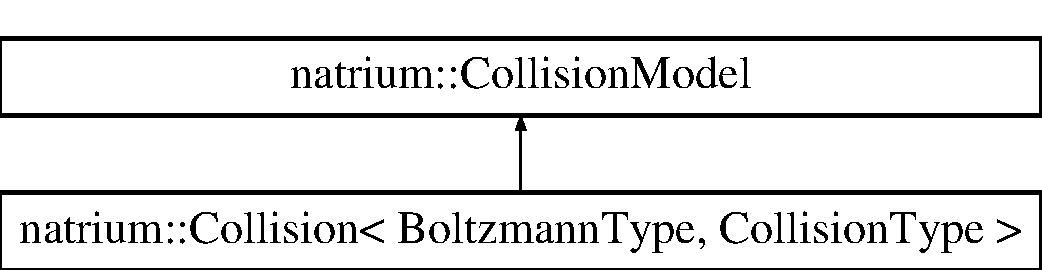
\includegraphics[height=2.000000cm]{classnatrium_1_1Collision}
\end{center}
\end{figure}
\subsection*{Public Member Functions}
\begin{DoxyCompactItemize}
\item 
\hyperlink{classnatrium_1_1Collision_a2a18af16681cbcea3ff0ebba132094f5}{Collision} (Boltzmann\-Type boltzmann\-Type, Collision\-Type collision\-Type)
\begin{DoxyCompactList}\small\item\em constructor, important\-: Copy arguments instead of reference \end{DoxyCompactList}\item 
\hypertarget{classnatrium_1_1Collision_aafa5f1a6f7da61df7c9ef54369dc8fed}{virtual \hyperlink{classnatrium_1_1Collision_aafa5f1a6f7da61df7c9ef54369dc8fed}{$\sim$\-Collision} ()}\label{classnatrium_1_1Collision_aafa5f1a6f7da61df7c9ef54369dc8fed}

\begin{DoxyCompactList}\small\item\em destructor \end{DoxyCompactList}\item 
\hypertarget{classnatrium_1_1Collision_ae6d6c234ac922a0602f4882ad19b4608}{virtual void \hyperlink{classnatrium_1_1Collision_ae6d6c234ac922a0602f4882ad19b4608}{collide\-Single\-Point} (vector$<$ double $>$ \&distributions) const }\label{classnatrium_1_1Collision_ae6d6c234ac922a0602f4882ad19b4608}

\begin{DoxyCompactList}\small\item\em only for testing purposes; do not use in code, because this function is very inefficient \end{DoxyCompactList}\item 
virtual void \hyperlink{classnatrium_1_1Collision_a5e1fe09430194ccb35bd2fcaa5958bf2}{collide\-All} (\hyperlink{classnatrium_1_1DistributionFunctions}{Distribution\-Functions} \&f, distributed\-\_\-vector \&densities, vector$<$ distributed\-\_\-vector $>$ \&velocities, const vector$<$ bool $>$ \&is\-Boundary, bool in\-Initialization\-Procedure=false) const 
\begin{DoxyCompactList}\small\item\em function for collision \end{DoxyCompactList}\item 
virtual void \hyperlink{classnatrium_1_1Collision_a12e3b507cbf329bbcc2bc8b9a184f6e2}{collide\-All} (\hyperlink{classnatrium_1_1DistributionFunctions}{Distribution\-Functions} \&f, distributed\-\_\-vector \&densities, vector$<$ distributed\-\_\-vector $>$ \&velocities, bool in\-Initialization\-Procedure=false) const 
\begin{DoxyCompactList}\small\item\em function for collision \end{DoxyCompactList}\item 
\hypertarget{classnatrium_1_1Collision_a978f4846827c2cf1129f560188807605}{{\footnotesize template$<$$>$ }\\void {\bfseries collide\-All} (\hyperlink{classnatrium_1_1DistributionFunctions}{Distribution\-Functions} \&f, distributed\-\_\-vector \&densities, vector$<$ distributed\-\_\-vector $>$ \&velocities, bool in\-Initialization\-Procedure) const}\label{classnatrium_1_1Collision_a978f4846827c2cf1129f560188807605}

\item 
\hypertarget{classnatrium_1_1Collision_a1a241ffb792c728a608580f9ab8dcb3d}{{\footnotesize template$<$$>$ }\\void {\bfseries collide\-All} (\hyperlink{classnatrium_1_1DistributionFunctions}{Distribution\-Functions} \&f, distributed\-\_\-vector \&densities, vector$<$ distributed\-\_\-vector $>$ \&velocities, bool in\-Initialization\-Procedure) const}\label{classnatrium_1_1Collision_a1a241ffb792c728a608580f9ab8dcb3d}

\end{DoxyCompactItemize}
\subsection*{Static Public Member Functions}
\begin{DoxyCompactItemize}
\item 
\hypertarget{classnatrium_1_1Collision_ad0ca1b0b33783e077d68b08892933f39}{static double \hyperlink{classnatrium_1_1Collision_ad0ca1b0b33783e077d68b08892933f39}{calculate\-Optimal\-Time\-Step} (double dx, const Boltzmann\-Type \&boltzmann\-Type)}\label{classnatrium_1_1Collision_ad0ca1b0b33783e077d68b08892933f39}

\begin{DoxyCompactList}\small\item\em calculate the time step, so that the Courant number is 1 for the diagonal directions \end{DoxyCompactList}\end{DoxyCompactItemize}
\subsection*{Protected Attributes}
\begin{DoxyCompactItemize}
\item 
\hypertarget{classnatrium_1_1Collision_aedbd709beac24029ee46002b123471a3}{const Boltzmann\-Type \hyperlink{classnatrium_1_1Collision_aedbd709beac24029ee46002b123471a3}{m\-\_\-boltzmann\-Type}}\label{classnatrium_1_1Collision_aedbd709beac24029ee46002b123471a3}

\begin{DoxyCompactList}\small\item\em Boltzmann model (e.\-g. D2\-Q9\-Incompressible) \end{DoxyCompactList}\item 
\hypertarget{classnatrium_1_1Collision_aae138b2fc3eb1a718a0b9bf3d75f9fd6}{const Collision\-Type {\bfseries m\-\_\-collision\-Type}}\label{classnatrium_1_1Collision_aae138b2fc3eb1a718a0b9bf3d75f9fd6}

\item 
\hypertarget{classnatrium_1_1Collision_ae4a33343ec73303ad63dfde4ac574cd6}{size\-\_\-t \hyperlink{classnatrium_1_1Collision_ae4a33343ec73303ad63dfde4ac574cd6}{m\-\_\-d}}\label{classnatrium_1_1Collision_ae4a33343ec73303ad63dfde4ac574cd6}

\begin{DoxyCompactList}\small\item\em D (dimension) \end{DoxyCompactList}\item 
\hypertarget{classnatrium_1_1Collision_a81cefcbe828514dbd71fe8ea8197724a}{double \hyperlink{classnatrium_1_1Collision_a81cefcbe828514dbd71fe8ea8197724a}{m\-\_\-q}}\label{classnatrium_1_1Collision_a81cefcbe828514dbd71fe8ea8197724a}

\begin{DoxyCompactList}\small\item\em Q (number of directions) \end{DoxyCompactList}\end{DoxyCompactItemize}


\subsection{Detailed Description}
\subsubsection*{template$<$class Boltzmann\-Type, class Collision\-Type$>$class natrium\-::\-Collision$<$ Boltzmann\-Type, Collision\-Type $>$}

Abstract class for the description of collision schemes. 

\subsection{Constructor \& Destructor Documentation}
\hypertarget{classnatrium_1_1Collision_a2a18af16681cbcea3ff0ebba132094f5}{\index{natrium\-::\-Collision@{natrium\-::\-Collision}!Collision@{Collision}}
\index{Collision@{Collision}!natrium::Collision@{natrium\-::\-Collision}}
\subsubsection[{Collision}]{\setlength{\rightskip}{0pt plus 5cm}template$<$class Boltzmann\-Type , class Collision\-Type $>$ template {\bf natrium\-::\-Collision}$<$ Boltzmann\-Type, Collision\-Type $>$\-::{\bf Collision} (
\begin{DoxyParamCaption}
\item[{Boltzmann\-Type}]{boltzmann\-Type, }
\item[{Collision\-Type}]{collision\-Type}
\end{DoxyParamCaption}
)}}\label{classnatrium_1_1Collision_a2a18af16681cbcea3ff0ebba132094f5}


constructor, important\-: Copy arguments instead of reference 


\begin{DoxyParams}[1]{Parameters}
\mbox{\tt in}  & {\em viscosity} & the kinematic viscosity \\
\hline
\mbox{\tt in}  & {\em time\-Step\-Size} & the size of the time step \\
\hline
\mbox{\tt in}  & {\em boltzmann\-Model} & the discrete velocity stencil \\
\hline
\end{DoxyParams}


\subsection{Member Function Documentation}
\hypertarget{classnatrium_1_1Collision_a5e1fe09430194ccb35bd2fcaa5958bf2}{\index{natrium\-::\-Collision@{natrium\-::\-Collision}!collide\-All@{collide\-All}}
\index{collide\-All@{collide\-All}!natrium::Collision@{natrium\-::\-Collision}}
\subsubsection[{collide\-All}]{\setlength{\rightskip}{0pt plus 5cm}template$<$class Boltzmann\-Type , class Collision\-Type $>$ template void {\bf natrium\-::\-Collision}$<$ Boltzmann\-Type, Collision\-Type $>$\-::collide\-All (
\begin{DoxyParamCaption}
\item[{{\bf Distribution\-Functions} \&}]{f, }
\item[{distributed\-\_\-vector \&}]{densities, }
\item[{vector$<$ distributed\-\_\-vector $>$ \&}]{velocities, }
\item[{const vector$<$ bool $>$ \&}]{is\-Boundary, }
\item[{bool}]{in\-Initialization\-Procedure = {\ttfamily false}}
\end{DoxyParamCaption}
) const\hspace{0.3cm}{\ttfamily [virtual]}}}\label{classnatrium_1_1Collision_a5e1fe09430194ccb35bd2fcaa5958bf2}


function for collision 

f the global vectors of discrete particle distribution functions densities the global vector of densities velocities the global vectors of velocity components \mbox{[} \mbox{[}u\-\_\-1x, u\-\_\-2x, ...\mbox{]}, \mbox{[}u\-\_\-1y, u\-\_\-2y, ...\mbox{]} \mbox{]} in\-Initialization\-Procedure indicates if the collision is performed in the context of an iterative initilizatation procedure. In this case, only the macroscopic densities are recalculated, while the velocities remain unchanged. default\-: false 

Implements \hyperlink{classnatrium_1_1CollisionModel}{natrium\-::\-Collision\-Model}.

\hypertarget{classnatrium_1_1Collision_a12e3b507cbf329bbcc2bc8b9a184f6e2}{\index{natrium\-::\-Collision@{natrium\-::\-Collision}!collide\-All@{collide\-All}}
\index{collide\-All@{collide\-All}!natrium::Collision@{natrium\-::\-Collision}}
\subsubsection[{collide\-All}]{\setlength{\rightskip}{0pt plus 5cm}template$<$class Boltzmann\-Type , class Collision\-Type $>$ void {\bf natrium\-::\-Collision}$<$ Boltzmann\-Type, Collision\-Type $>$\-::collide\-All (
\begin{DoxyParamCaption}
\item[{{\bf Distribution\-Functions} \&}]{f, }
\item[{distributed\-\_\-vector \&}]{densities, }
\item[{vector$<$ distributed\-\_\-vector $>$ \&}]{velocities, }
\item[{bool}]{in\-Initialization\-Procedure = {\ttfamily false}}
\end{DoxyParamCaption}
) const\hspace{0.3cm}{\ttfamily [virtual]}}}\label{classnatrium_1_1Collision_a12e3b507cbf329bbcc2bc8b9a184f6e2}


function for collision 

f the global vectors of discrete particle distribution functions densities the global vector of densities velocities the global vectors of velocity components \mbox{[} \mbox{[}u\-\_\-1x, u\-\_\-2x, ...\mbox{]}, \mbox{[}u\-\_\-1y, u\-\_\-2y, ...\mbox{]} \mbox{]} in\-Initialization\-Procedure indicates if the collision is performed in the context of an iterative initilizatation procedure. In this case, only the macroscopic densities are recalculated, while the velocities remain unchanged. default\-: false 

Implements \hyperlink{classnatrium_1_1CollisionModel}{natrium\-::\-Collision\-Model}.



The documentation for this class was generated from the following files\-:\begin{DoxyCompactItemize}
\item 
/home/kraemer/eclipse\-\_\-workspace/\-N\-A\-Triu\-M/src/natrium/collision/Collision.\-h\item 
/home/kraemer/eclipse\-\_\-workspace/\-N\-A\-Triu\-M/src/natrium/collision/Collision.\-cpp\end{DoxyCompactItemize}

\hypertarget{classnatrium_1_1CollisionException}{\section{natrium\-:\-:Collision\-Exception Class Reference}
\label{classnatrium_1_1CollisionException}\index{natrium\-::\-Collision\-Exception@{natrium\-::\-Collision\-Exception}}
}


Exception class for \hyperlink{classnatrium_1_1Collision}{Collision} model.  




{\ttfamily \#include $<$Collision.\-h$>$}

Inheritance diagram for natrium\-:\-:Collision\-Exception\-:\begin{figure}[H]
\begin{center}
\leavevmode
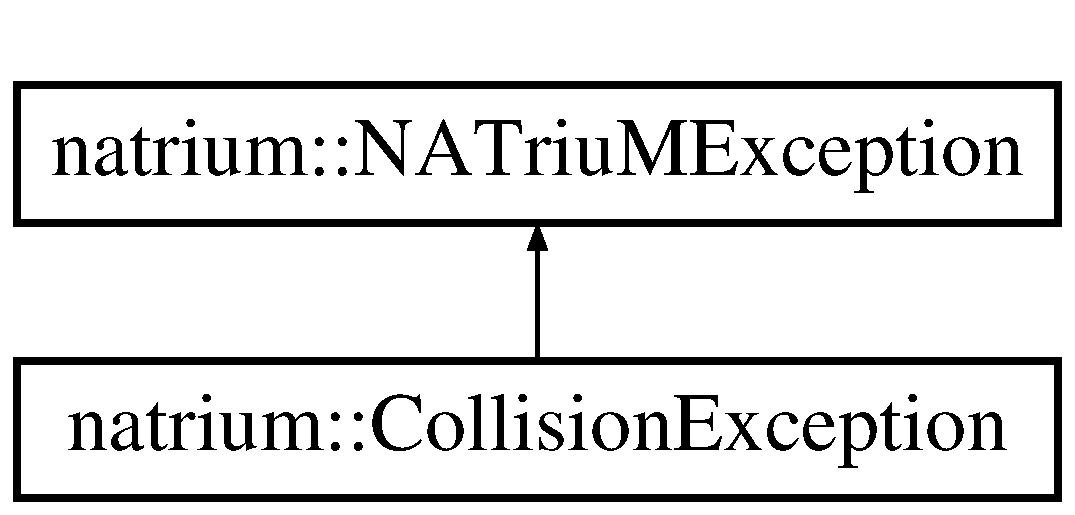
\includegraphics[height=2.000000cm]{classnatrium_1_1CollisionException}
\end{center}
\end{figure}
\subsection*{Public Member Functions}
\begin{DoxyCompactItemize}
\item 
\hypertarget{classnatrium_1_1CollisionException_aee60989a43066bd65b0481cde4d96980}{{\bfseries Collision\-Exception} (const char $\ast$msg)}\label{classnatrium_1_1CollisionException_aee60989a43066bd65b0481cde4d96980}

\item 
\hypertarget{classnatrium_1_1CollisionException_a700f9ee10ef668a35cb227d8a7b01d4c}{const char $\ast$ {\bfseries what} () const   throw ()}\label{classnatrium_1_1CollisionException_a700f9ee10ef668a35cb227d8a7b01d4c}

\end{DoxyCompactItemize}


\subsection{Detailed Description}
Exception class for \hyperlink{classnatrium_1_1Collision}{Collision} model. 

The documentation for this class was generated from the following file\-:\begin{DoxyCompactItemize}
\item 
/home/kraemer/eclipse\-\_\-workspace/\-N\-A\-Triu\-M/src/natrium/collision/Collision.\-h\end{DoxyCompactItemize}

\hypertarget{classnatrium_1_1CollisionModel}{
\section{natrium::CollisionModel Class Reference}
\label{classnatrium_1_1CollisionModel}\index{natrium::CollisionModel@{natrium::CollisionModel}}
}


Abstract collision model. Required to have a common parent of all template specializations of Collision.  


{\ttfamily \#include $<$CollisionModel.h$>$}Inheritance diagram for natrium::CollisionModel::\begin{figure}[H]
\begin{center}
\leavevmode
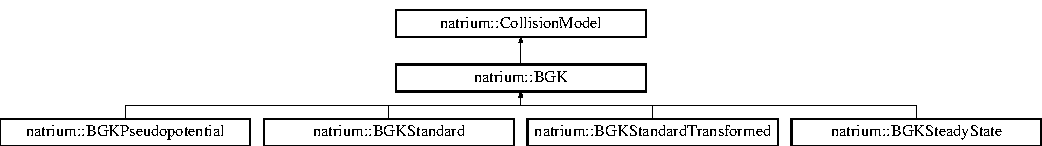
\includegraphics[height=1.96262cm]{classnatrium_1_1CollisionModel}
\end{center}
\end{figure}
\subsection*{Public Member Functions}
\begin{DoxyCompactItemize}
\item 
\hypertarget{classnatrium_1_1CollisionModel_a5e5254caec7f69000646886be11a34f8}{
{\bfseries CollisionModel} (const shared\_\-ptr$<$ \hyperlink{classnatrium_1_1Stencil}{Stencil} $>$ stencil)}
\label{classnatrium_1_1CollisionModel_a5e5254caec7f69000646886be11a34f8}

\item 
\hypertarget{classnatrium_1_1CollisionModel_ac6c6d95633d62209a04528af86807025}{
virtual void {\bfseries collideAll} (\hyperlink{classnatrium_1_1DistributionFunctions}{DistributionFunctions} \&f, distributed\_\-vector \&densities, vector$<$ distributed\_\-vector $>$ \&velocities, const dealii::IndexSet \&locally\_\-owned\_\-dofs, bool inInitializationProcedure=false) const =0}
\label{classnatrium_1_1CollisionModel_ac6c6d95633d62209a04528af86807025}

\item 
\hypertarget{classnatrium_1_1CollisionModel_aa0df0674bc26821d037323ac184fb52b}{
virtual void {\bfseries setTimeStep} (double dt)=0}
\label{classnatrium_1_1CollisionModel_aa0df0674bc26821d037323ac184fb52b}

\item 
\hypertarget{classnatrium_1_1CollisionModel_a482808bab1832ee06892630b8ead7dde}{
const shared\_\-ptr$<$ \hyperlink{classnatrium_1_1Stencil}{Stencil} $>$ \& {\bfseries getStencil} () const }
\label{classnatrium_1_1CollisionModel_a482808bab1832ee06892630b8ead7dde}

\item 
virtual double \hyperlink{classnatrium_1_1CollisionModel_ae1c879c87ac210a227a8e3da2d0ac385}{calculateDensity} (const vector$<$ double $>$ \&distributions) const 
\begin{DoxyCompactList}\small\item\em calculate macroscopic density \item\end{DoxyCompactList}\item 
virtual numeric\_\-vector \hyperlink{classnatrium_1_1CollisionModel_a90428f4c29916641de3de872803dde0f}{calculateVelocity} (const vector$<$ double $>$ \&distributions) const 
\begin{DoxyCompactList}\small\item\em calculate macroscopic velocity \item\end{DoxyCompactList}\item 
virtual void \hyperlink{classnatrium_1_1CollisionModel_a667f0e36da1bfb1c5102adb8f3afdcde}{calculateVelocity} (const vector$<$ double $>$ \&distributions, const double rho, numeric\_\-vector \&u) const 
\begin{DoxyCompactList}\small\item\em calculate macroscopic velocity; saves the double calculation of the density \item\end{DoxyCompactList}\item 
virtual double \hyperlink{classnatrium_1_1CollisionModel_a88b382d63da80e950bc58e8afad769a6}{getEquilibriumDistribution} (size\_\-t i, const numeric\_\-vector \&u, const double rho=1) const =0
\begin{DoxyCompactList}\small\item\em virtual function for the calculation of the equilibrium distribution \item\end{DoxyCompactList}\item 
virtual void \hyperlink{classnatrium_1_1CollisionModel_a296474961c4501bc23228be1d30ebf82}{getEquilibriumDistributions} (vector$<$ double $>$ \&feq, const numeric\_\-vector \&u, const double rho=1) const 
\begin{DoxyCompactList}\small\item\em function for the calculation of all equilibrium distributions \item\end{DoxyCompactList}\end{DoxyCompactItemize}


\subsection{Detailed Description}
Abstract collision model. Required to have a common parent of all template specializations of Collision. 

\subsection{Member Function Documentation}
\hypertarget{classnatrium_1_1CollisionModel_ae1c879c87ac210a227a8e3da2d0ac385}{
\index{natrium::CollisionModel@{natrium::CollisionModel}!calculateDensity@{calculateDensity}}
\index{calculateDensity@{calculateDensity}!natrium::CollisionModel@{natrium::CollisionModel}}
\subsubsection[{calculateDensity}]{\setlength{\rightskip}{0pt plus 5cm}virtual double natrium::CollisionModel::calculateDensity (const vector$<$ double $>$ \& {\em distributions}) const\hspace{0.3cm}{\ttfamily  \mbox{[}inline, virtual\mbox{]}}}}
\label{classnatrium_1_1CollisionModel_ae1c879c87ac210a227a8e3da2d0ac385}


calculate macroscopic density 
\begin{DoxyParams}{Parameters}
\item[\mbox{$\leftarrow$} {\em distributions}]particle distribution functions at a given point \end{DoxyParams}
\begin{DoxyReturn}{Returns}
macroscopic density (sum of all distributions) 
\end{DoxyReturn}


Reimplemented in \hyperlink{classnatrium_1_1BGKStandardTransformed_a58c4dc0c67ff4898c6555b614afc1ace}{natrium::BGKStandardTransformed}.\hypertarget{classnatrium_1_1CollisionModel_a667f0e36da1bfb1c5102adb8f3afdcde}{
\index{natrium::CollisionModel@{natrium::CollisionModel}!calculateVelocity@{calculateVelocity}}
\index{calculateVelocity@{calculateVelocity}!natrium::CollisionModel@{natrium::CollisionModel}}
\subsubsection[{calculateVelocity}]{\setlength{\rightskip}{0pt plus 5cm}virtual void natrium::CollisionModel::calculateVelocity (const vector$<$ double $>$ \& {\em distributions}, \/  const double {\em rho}, \/  numeric\_\-vector \& {\em u}) const\hspace{0.3cm}{\ttfamily  \mbox{[}inline, virtual\mbox{]}}}}
\label{classnatrium_1_1CollisionModel_a667f0e36da1bfb1c5102adb8f3afdcde}


calculate macroscopic velocity; saves the double calculation of the density \begin{DoxyNote}{Note}
more efficient 
\end{DoxyNote}

\begin{DoxyParams}{Parameters}
\item[\mbox{$\leftarrow$} {\em distributions}]particle distribution functions at a given point \item[\mbox{$\leftarrow$} {\em rho}]macroscopic density \item[\mbox{$\rightarrow$} {\em u}]macroscopic velocity \end{DoxyParams}
\hypertarget{classnatrium_1_1CollisionModel_a90428f4c29916641de3de872803dde0f}{
\index{natrium::CollisionModel@{natrium::CollisionModel}!calculateVelocity@{calculateVelocity}}
\index{calculateVelocity@{calculateVelocity}!natrium::CollisionModel@{natrium::CollisionModel}}
\subsubsection[{calculateVelocity}]{\setlength{\rightskip}{0pt plus 5cm}virtual numeric\_\-vector natrium::CollisionModel::calculateVelocity (const vector$<$ double $>$ \& {\em distributions}) const\hspace{0.3cm}{\ttfamily  \mbox{[}inline, virtual\mbox{]}}}}
\label{classnatrium_1_1CollisionModel_a90428f4c29916641de3de872803dde0f}


calculate macroscopic velocity 
\begin{DoxyParams}{Parameters}
\item[\mbox{$\leftarrow$} {\em distributions}]particle distribution functions at a given point \end{DoxyParams}
\begin{DoxyReturn}{Returns}
macroscopic velocity 
\end{DoxyReturn}
\hypertarget{classnatrium_1_1CollisionModel_a88b382d63da80e950bc58e8afad769a6}{
\index{natrium::CollisionModel@{natrium::CollisionModel}!getEquilibriumDistribution@{getEquilibriumDistribution}}
\index{getEquilibriumDistribution@{getEquilibriumDistribution}!natrium::CollisionModel@{natrium::CollisionModel}}
\subsubsection[{getEquilibriumDistribution}]{\setlength{\rightskip}{0pt plus 5cm}virtual double natrium::CollisionModel::getEquilibriumDistribution (size\_\-t {\em i}, \/  const numeric\_\-vector \& {\em u}, \/  const double {\em rho} = {\ttfamily 1}) const\hspace{0.3cm}{\ttfamily  \mbox{[}pure virtual\mbox{]}}}}
\label{classnatrium_1_1CollisionModel_a88b382d63da80e950bc58e8afad769a6}


virtual function for the calculation of the equilibrium distribution 
\begin{DoxyParams}{Parameters}
\item[{\em i}]index of the direction \item[{\em u}]macroscopic velocity \item[{\em rho}]macroscopic density \end{DoxyParams}
\begin{DoxyReturn}{Returns}
value of the equilibrium distribution 
\end{DoxyReturn}
\begin{DoxyNote}{Note}
The calculation can surely be done more efficiently by passing different arguments, e.g. u$\ast$u or u/(c$^\wedge$2) 
\end{DoxyNote}


Implemented in \hyperlink{classnatrium_1_1BGKPseudopotential_a63ce98e44a07466963fb123cac9dd905}{natrium::BGKPseudopotential}, \hyperlink{classnatrium_1_1BGKStandard_a3d45ef2fe5536bf14914f99297477754}{natrium::BGKStandard}, \hyperlink{classnatrium_1_1BGKStandardTransformed_a870465cc026f92c8ffba899af6f95634}{natrium::BGKStandardTransformed}, and \hyperlink{classnatrium_1_1BGKSteadyState_ad99d9159cc14b5897bea7f145c3b39ca}{natrium::BGKSteadyState}.\hypertarget{classnatrium_1_1CollisionModel_a296474961c4501bc23228be1d30ebf82}{
\index{natrium::CollisionModel@{natrium::CollisionModel}!getEquilibriumDistributions@{getEquilibriumDistributions}}
\index{getEquilibriumDistributions@{getEquilibriumDistributions}!natrium::CollisionModel@{natrium::CollisionModel}}
\subsubsection[{getEquilibriumDistributions}]{\setlength{\rightskip}{0pt plus 5cm}void natrium::CollisionModel::getEquilibriumDistributions (vector$<$ double $>$ \& {\em feq}, \/  const numeric\_\-vector \& {\em u}, \/  const double {\em rho} = {\ttfamily 1}) const\hspace{0.3cm}{\ttfamily  \mbox{[}virtual\mbox{]}}}}
\label{classnatrium_1_1CollisionModel_a296474961c4501bc23228be1d30ebf82}


function for the calculation of all equilibrium distributions 
\begin{DoxyParams}{Parameters}
\item[\mbox{$\rightarrow$} {\em feq}]vector of all equality distributions, must have size Q \item[\mbox{$\leftarrow$} {\em u}]macroscopic velocity \item[\mbox{$\leftarrow$} {\em rho}]macroscopic density \end{DoxyParams}
\begin{DoxyNote}{Note}
The calculation can surely be done more efficiently by passing different arguments, e.g. u$\ast$u or u/(c$^\wedge$2) 
\end{DoxyNote}


The documentation for this class was generated from the following files:\begin{DoxyCompactItemize}
\item 
/mnt/fdrive/akraem3m/workspace/NATriuM/src/library/natrium/collision/\hyperlink{CollisionModel_8h}{CollisionModel.h}\item 
/mnt/fdrive/akraem3m/workspace/NATriuM/src/library/natrium/collision/\hyperlink{CollisionModel_8cpp}{CollisionModel.cpp}\end{DoxyCompactItemize}

\hypertarget{classnatrium_1_1ComplexWall1}{\section{natrium\-:\-:Complex\-Wall1 Class Reference}
\label{classnatrium_1_1ComplexWall1}\index{natrium\-::\-Complex\-Wall1@{natrium\-::\-Complex\-Wall1}}
}


Description of a simple Couette Flow (regular channel flow in square domain). The domain is \mbox{[}0,1\mbox{]}$^\wedge$2. The top plate is moved with constant velocity. The domain consists of 8 x 8 = 64 Elements (contrast to Min and Lee, who have 6 x 6).  




{\ttfamily \#include $<$Complex\-Wall1.\-h$>$}

Inheritance diagram for natrium\-:\-:Complex\-Wall1\-:\begin{figure}[H]
\begin{center}
\leavevmode
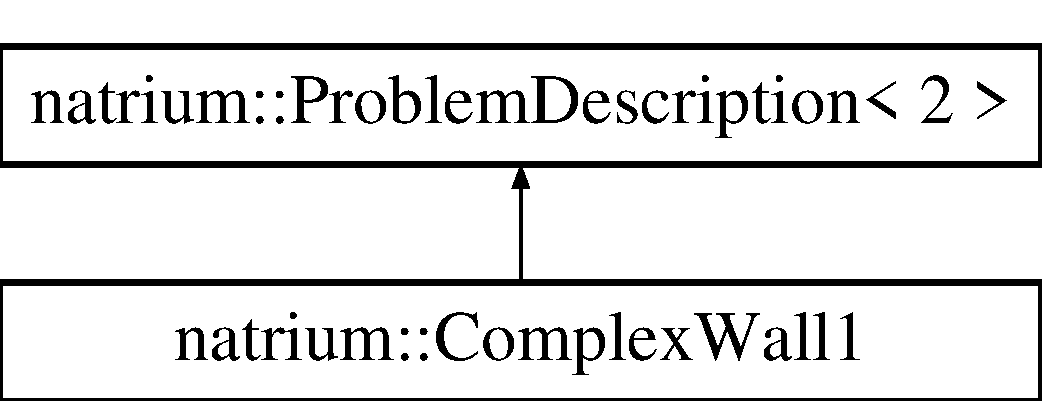
\includegraphics[height=2.000000cm]{classnatrium_1_1ComplexWall1}
\end{center}
\end{figure}
\subsection*{Public Member Functions}
\begin{DoxyCompactItemize}
\item 
\hyperlink{classnatrium_1_1ComplexWall1_ad619c81f979a47c447fc0061bed20e05}{Complex\-Wall1} (double viscosity, double bottom\-Velocity, size\-\_\-t refinement\-Level, double L=1.\-0)
\begin{DoxyCompactList}\small\item\em constructor \end{DoxyCompactList}\item 
\hypertarget{classnatrium_1_1ComplexWall1_a6d68cdec98529c139716ae98e8149d30}{virtual \hyperlink{classnatrium_1_1ComplexWall1_a6d68cdec98529c139716ae98e8149d30}{$\sim$\-Complex\-Wall1} ()}\label{classnatrium_1_1ComplexWall1_a6d68cdec98529c139716ae98e8149d30}

\begin{DoxyCompactList}\small\item\em destructor \end{DoxyCompactList}\item 
\hypertarget{classnatrium_1_1ComplexWall1_a782e4262d5c717656803f43eb4e05202}{virtual double {\bfseries get\-Characteristic\-Velocity} () const }\label{classnatrium_1_1ComplexWall1_a782e4262d5c717656803f43eb4e05202}

\end{DoxyCompactItemize}


\subsection{Detailed Description}
Description of a simple Couette Flow (regular channel flow in square domain). The domain is \mbox{[}0,1\mbox{]}$^\wedge$2. The top plate is moved with constant velocity. The domain consists of 8 x 8 = 64 Elements (contrast to Min and Lee, who have 6 x 6). 

\begin{DoxyNote}{Note}
The analytic solution is obtained by a formula stated in Min and Lee (2011). 
\end{DoxyNote}


\subsection{Constructor \& Destructor Documentation}
\hypertarget{classnatrium_1_1ComplexWall1_ad619c81f979a47c447fc0061bed20e05}{\index{natrium\-::\-Complex\-Wall1@{natrium\-::\-Complex\-Wall1}!Complex\-Wall1@{Complex\-Wall1}}
\index{Complex\-Wall1@{Complex\-Wall1}!natrium::ComplexWall1@{natrium\-::\-Complex\-Wall1}}
\subsubsection[{Complex\-Wall1}]{\setlength{\rightskip}{0pt plus 5cm}natrium\-::\-Complex\-Wall1\-::\-Complex\-Wall1 (
\begin{DoxyParamCaption}
\item[{double}]{viscosity, }
\item[{double}]{bottom\-Velocity, }
\item[{size\-\_\-t}]{refinement\-Level, }
\item[{double}]{L = {\ttfamily 1.0}}
\end{DoxyParamCaption}
)}}\label{classnatrium_1_1ComplexWall1_ad619c81f979a47c447fc0061bed20e05}


constructor 

apply boundary values 

The documentation for this class was generated from the following files\-:\begin{DoxyCompactItemize}
\item 
/home/kraemer/eclipse\-\_\-workspace/\-N\-A\-Triu\-M/src/examples/step-\/6/Complex\-Wall1.\-h\item 
/home/kraemer/eclipse\-\_\-workspace/\-N\-A\-Triu\-M/src/examples/step-\/6/\hyperlink{ComplexWall1_8cpp}{Complex\-Wall1.\-cpp}\end{DoxyCompactItemize}

\hypertarget{classnatrium_1_1ConfigurationException}{\section{natrium\-:\-:Configuration\-Exception Class Reference}
\label{classnatrium_1_1ConfigurationException}\index{natrium\-::\-Configuration\-Exception@{natrium\-::\-Configuration\-Exception}}
}


Exception class for \hyperlink{classnatrium_1_1CFDSolver}{C\-F\-D\-Solver}.  




{\ttfamily \#include $<$Solver\-Configuration.\-h$>$}

Inheritance diagram for natrium\-:\-:Configuration\-Exception\-:\begin{figure}[H]
\begin{center}
\leavevmode
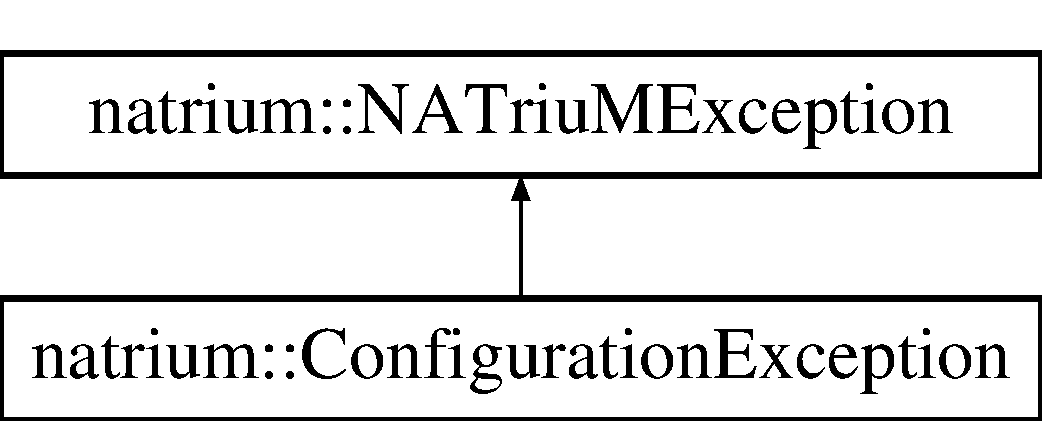
\includegraphics[height=2.000000cm]{classnatrium_1_1ConfigurationException}
\end{center}
\end{figure}
\subsection*{Public Member Functions}
\begin{DoxyCompactItemize}
\item 
\hypertarget{classnatrium_1_1ConfigurationException_ac9248a6224570c873784f201ef9ae34f}{{\bfseries Configuration\-Exception} (const char $\ast$msg)}\label{classnatrium_1_1ConfigurationException_ac9248a6224570c873784f201ef9ae34f}

\item 
\hypertarget{classnatrium_1_1ConfigurationException_a9f622f88d955e5c5e01719b7fcb273a6}{{\bfseries Configuration\-Exception} (const string \&msg)}\label{classnatrium_1_1ConfigurationException_a9f622f88d955e5c5e01719b7fcb273a6}

\item 
\hypertarget{classnatrium_1_1ConfigurationException_a48c72bd9bbae81e098a1f214899b3de6}{const char $\ast$ {\bfseries what} () const   throw ()}\label{classnatrium_1_1ConfigurationException_a48c72bd9bbae81e098a1f214899b3de6}

\end{DoxyCompactItemize}


\subsection{Detailed Description}
Exception class for \hyperlink{classnatrium_1_1CFDSolver}{C\-F\-D\-Solver}. 

The documentation for this class was generated from the following file\-:\begin{DoxyCompactItemize}
\item 
/home/kraemer/eclipse\-\_\-workspace/\-N\-A\-Triu\-M/src/natrium/solver/\hyperlink{SolverConfiguration_8h}{Solver\-Configuration.\-h}\end{DoxyCompactItemize}

\hypertarget{classnatrium_1_1CouetteFlow2D}{\section{natrium\-:\-:Couette\-Flow2\-D Class Reference}
\label{classnatrium_1_1CouetteFlow2D}\index{natrium\-::\-Couette\-Flow2\-D@{natrium\-::\-Couette\-Flow2\-D}}
}


Description of a simple Couette Flow (regular channel flow in square domain). The domain is \mbox{[}0,1\mbox{]}$^\wedge$2. The top plate is moved with constant velocity. The domain consists of 8 x 8 = 64 Elements (contrast to Min and Lee, who have 6 x 6).  




{\ttfamily \#include $<$Couette\-Flow2\-D.\-h$>$}

Inheritance diagram for natrium\-:\-:Couette\-Flow2\-D\-:\begin{figure}[H]
\begin{center}
\leavevmode
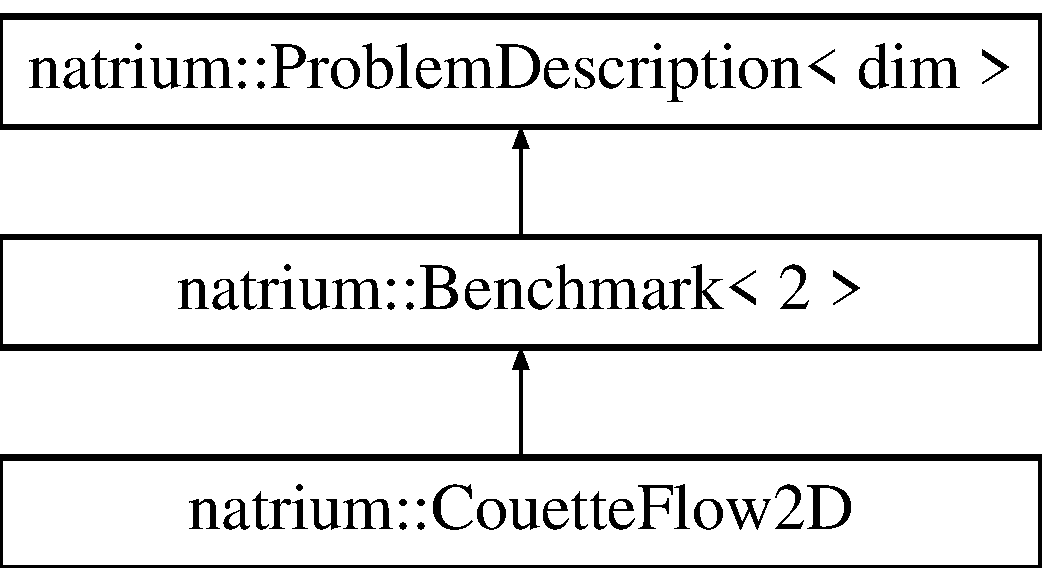
\includegraphics[height=3.000000cm]{classnatrium_1_1CouetteFlow2D}
\end{center}
\end{figure}
\subsection*{Public Member Functions}
\begin{DoxyCompactItemize}
\item 
\hyperlink{classnatrium_1_1CouetteFlow2D_a94e51b7eaff3998383f1d7dc07b994cb}{Couette\-Flow2\-D} (double viscosity, double top\-Plate\-Velocity, size\-\_\-t refinement\-Level, double L=1.\-0, double start\-Time=0.\-0, bool is\-Unstructured=false)
\begin{DoxyCompactList}\small\item\em constructor \end{DoxyCompactList}\item 
\hypertarget{classnatrium_1_1CouetteFlow2D_a97b61b0f71dc653427ba3db46e185873}{virtual \hyperlink{classnatrium_1_1CouetteFlow2D_a97b61b0f71dc653427ba3db46e185873}{$\sim$\-Couette\-Flow2\-D} ()}\label{classnatrium_1_1CouetteFlow2D_a97b61b0f71dc653427ba3db46e185873}

\begin{DoxyCompactList}\small\item\em destructor \end{DoxyCompactList}\item 
\hypertarget{classnatrium_1_1CouetteFlow2D_a3953d81acbab33424dfc4135930253df}{virtual void \hyperlink{classnatrium_1_1CouetteFlow2D_a3953d81acbab33424dfc4135930253df}{get\-Analytic\-Velocity} (const dealii\-::\-Point$<$ 2 $>$ \&x, double t, dealii\-::\-Point$<$ 2 $>$ \&velocity) const }\label{classnatrium_1_1CouetteFlow2D_a3953d81acbab33424dfc4135930253df}

\begin{DoxyCompactList}\small\item\em analytic solution of the Taylor-\/\-Green vortex \end{DoxyCompactList}\item 
\hypertarget{classnatrium_1_1CouetteFlow2D_a74429d98c455a0c06430a665505d8375}{virtual double {\bfseries get\-Characteristic\-Velocity} () const }\label{classnatrium_1_1CouetteFlow2D_a74429d98c455a0c06430a665505d8375}

\end{DoxyCompactItemize}


\subsection{Detailed Description}
Description of a simple Couette Flow (regular channel flow in square domain). The domain is \mbox{[}0,1\mbox{]}$^\wedge$2. The top plate is moved with constant velocity. The domain consists of 8 x 8 = 64 Elements (contrast to Min and Lee, who have 6 x 6). 

\begin{DoxyNote}{Note}
The analytic solution is obtained by a formula stated in Min and Lee (2011). 
\end{DoxyNote}


\subsection{Constructor \& Destructor Documentation}
\hypertarget{classnatrium_1_1CouetteFlow2D_a94e51b7eaff3998383f1d7dc07b994cb}{\index{natrium\-::\-Couette\-Flow2\-D@{natrium\-::\-Couette\-Flow2\-D}!Couette\-Flow2\-D@{Couette\-Flow2\-D}}
\index{Couette\-Flow2\-D@{Couette\-Flow2\-D}!natrium::CouetteFlow2D@{natrium\-::\-Couette\-Flow2\-D}}
\subsubsection[{Couette\-Flow2\-D}]{\setlength{\rightskip}{0pt plus 5cm}natrium\-::\-Couette\-Flow2\-D\-::\-Couette\-Flow2\-D (
\begin{DoxyParamCaption}
\item[{double}]{viscosity, }
\item[{double}]{top\-Plate\-Velocity, }
\item[{size\-\_\-t}]{refinement\-Level, }
\item[{double}]{L = {\ttfamily 1.0}, }
\item[{double}]{start\-Time = {\ttfamily 0.0}, }
\item[{bool}]{is\-Unstructured = {\ttfamily false}}
\end{DoxyParamCaption}
)}}\label{classnatrium_1_1CouetteFlow2D_a94e51b7eaff3998383f1d7dc07b994cb}


constructor 

apply boundary values 

The documentation for this class was generated from the following files\-:\begin{DoxyCompactItemize}
\item 
/home/kraemer/eclipse\-\_\-workspace/\-N\-A\-Triu\-M/src/examples/step-\/2/\hyperlink{CouetteFlow2D_8h}{Couette\-Flow2\-D.\-h}\item 
/home/kraemer/eclipse\-\_\-workspace/\-N\-A\-Triu\-M/src/examples/step-\/2/\hyperlink{CouetteFlow2D_8cpp}{Couette\-Flow2\-D.\-cpp}\end{DoxyCompactItemize}

\hypertarget{classnatrium_1_1Cylinder2D}{
\section{natrium::Cylinder2D Class Reference}
\label{classnatrium_1_1Cylinder2D}\index{natrium::Cylinder2D@{natrium::Cylinder2D}}
}


Description of the flow around a circular cylinder (regular channel flow in square domain).  


{\ttfamily \#include $<$Cylinder2D.h$>$}Inheritance diagram for natrium::Cylinder2D::\begin{figure}[H]
\begin{center}
\leavevmode
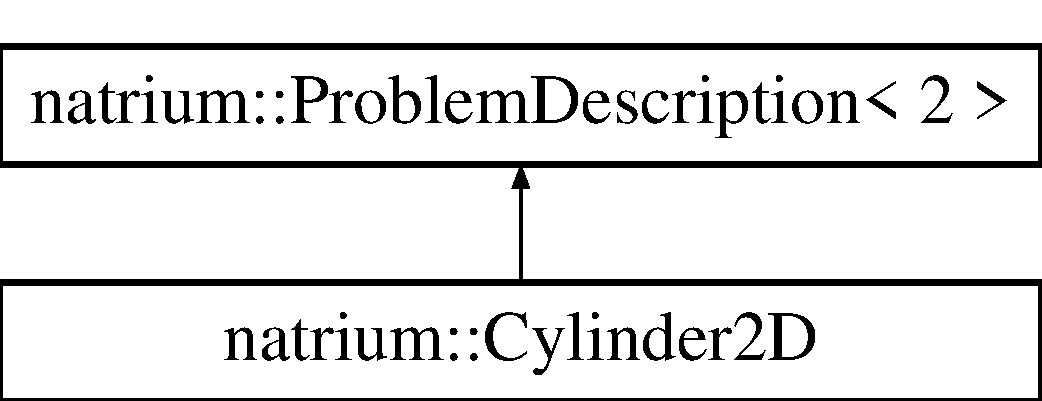
\includegraphics[height=2cm]{classnatrium_1_1Cylinder2D}
\end{center}
\end{figure}
\subsection*{Public Member Functions}
\begin{DoxyCompactItemize}
\item 
\hyperlink{classnatrium_1_1Cylinder2D_a38e5826b6fd4fc859b74783de3999658}{Cylinder2D} (double viscosity, double inletVelocity)
\begin{DoxyCompactList}\small\item\em constructor \item\end{DoxyCompactList}\item 
\hypertarget{classnatrium_1_1Cylinder2D_a40a33168f7deb7f35e4eb7b3f749b4a3}{
virtual \hyperlink{classnatrium_1_1Cylinder2D_a40a33168f7deb7f35e4eb7b3f749b4a3}{$\sim$Cylinder2D} ()}
\label{classnatrium_1_1Cylinder2D_a40a33168f7deb7f35e4eb7b3f749b4a3}

\begin{DoxyCompactList}\small\item\em destructor \item\end{DoxyCompactList}\item 
\hypertarget{classnatrium_1_1Cylinder2D_a6e32e2b875af680163160779aca52134}{
virtual double {\bfseries getCharacteristicVelocity} () const }
\label{classnatrium_1_1Cylinder2D_a6e32e2b875af680163160779aca52134}

\item 
\hypertarget{classnatrium_1_1Cylinder2D_aa67c905852893276844a6f9d6013cc05}{
virtual void {\bfseries refine} (Mesh$<$ 2 $>$ \&mesh)}
\label{classnatrium_1_1Cylinder2D_aa67c905852893276844a6f9d6013cc05}

\item 
\hypertarget{classnatrium_1_1Cylinder2D_a34077d9eecf1277adc4e7255ed695fc0}{
virtual void {\bfseries transform} (Mesh$<$ 2 $>$ \&mesh)}
\label{classnatrium_1_1Cylinder2D_a34077d9eecf1277adc4e7255ed695fc0}

\end{DoxyCompactItemize}


\subsection{Detailed Description}
Description of the flow around a circular cylinder (regular channel flow in square domain). 

\subsection{Constructor \& Destructor Documentation}
\hypertarget{classnatrium_1_1Cylinder2D_a38e5826b6fd4fc859b74783de3999658}{
\index{natrium::Cylinder2D@{natrium::Cylinder2D}!Cylinder2D@{Cylinder2D}}
\index{Cylinder2D@{Cylinder2D}!natrium::Cylinder2D@{natrium::Cylinder2D}}
\subsubsection[{Cylinder2D}]{\setlength{\rightskip}{0pt plus 5cm}natrium::Cylinder2D::Cylinder2D (double {\em viscosity}, \/  double {\em inletVelocity})}}
\label{classnatrium_1_1Cylinder2D_a38e5826b6fd4fc859b74783de3999658}


constructor 

apply boundary values 

The documentation for this class was generated from the following files:\begin{DoxyCompactItemize}
\item 
/mnt/fdrive/akraem3m/workspace/NATriuM/src/examples/step-\/9/\hyperlink{Cylinder2D_8h}{Cylinder2D.h}\item 
/mnt/fdrive/akraem3m/workspace/NATriuM/src/examples/step-\/9/\hyperlink{Cylinder2D_8cpp}{Cylinder2D.cpp}\end{DoxyCompactItemize}

\hypertarget{classnatrium_1_1D2Q9IncompressibleModel}{\section{natrium\-:\-:D2\-Q9\-Incompressible\-Model Class Reference}
\label{classnatrium_1_1D2Q9IncompressibleModel}\index{natrium\-::\-D2\-Q9\-Incompressible\-Model@{natrium\-::\-D2\-Q9\-Incompressible\-Model}}
}


D2\-Q9 model description for incompressible flow.  




{\ttfamily \#include $<$D2\-Q9\-Incompressible\-Model.\-h$>$}

Inheritance diagram for natrium\-:\-:D2\-Q9\-Incompressible\-Model\-:\begin{figure}[H]
\begin{center}
\leavevmode
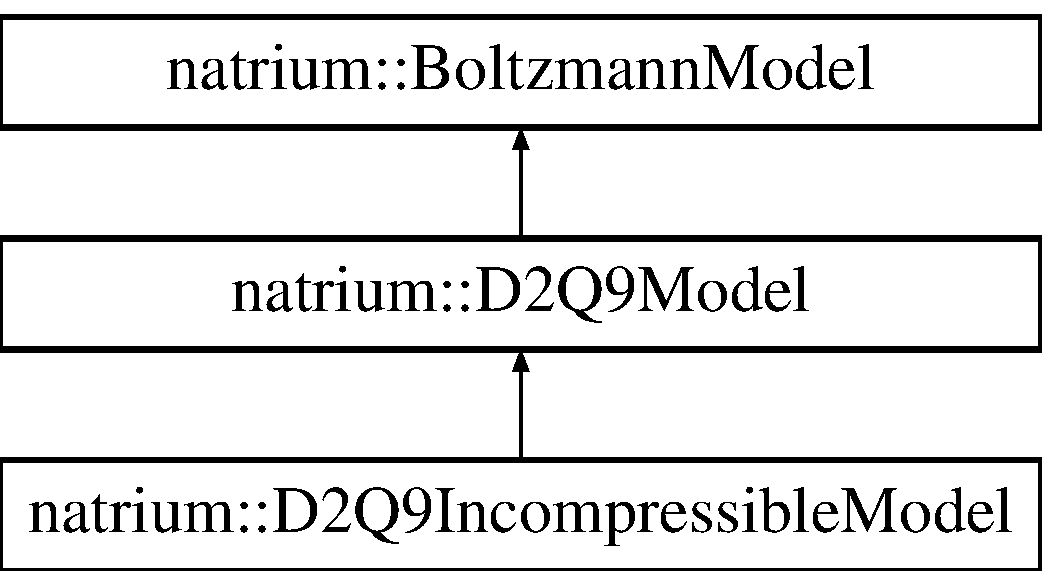
\includegraphics[height=3.000000cm]{classnatrium_1_1D2Q9IncompressibleModel}
\end{center}
\end{figure}
\subsection*{Public Member Functions}
\begin{DoxyCompactItemize}
\item 
\hypertarget{classnatrium_1_1D2Q9IncompressibleModel_a2ebdd3442edd4e3f38798a99b8413fcb}{\hyperlink{classnatrium_1_1D2Q9IncompressibleModel_a2ebdd3442edd4e3f38798a99b8413fcb}{D2\-Q9\-Incompressible\-Model} (double scaling=1)}\label{classnatrium_1_1D2Q9IncompressibleModel_a2ebdd3442edd4e3f38798a99b8413fcb}

\begin{DoxyCompactList}\small\item\em constructor \end{DoxyCompactList}\item 
virtual \hyperlink{classnatrium_1_1D2Q9IncompressibleModel_a6e757941f7ca2c5a6148893147211724}{$\sim$\-D2\-Q9\-Incompressible\-Model} ()
\begin{DoxyCompactList}\small\item\em destructor \end{DoxyCompactList}\item 
virtual double \hyperlink{classnatrium_1_1D2Q9IncompressibleModel_ac461ec3ce0f4ecd742dfbdfb1bce7d5a}{get\-Equilibrium\-Distribution} (size\-\_\-t i, const numeric\-\_\-vector \&u, const double rho=1) const 
\begin{DoxyCompactList}\small\item\em function for the calculation of the equilibrium distribution in the incompressible D2\-Q9 model \end{DoxyCompactList}\end{DoxyCompactItemize}
\subsection*{Additional Inherited Members}


\subsection{Detailed Description}
D2\-Q9 model description for incompressible flow. 

\subsection{Constructor \& Destructor Documentation}
\hypertarget{classnatrium_1_1D2Q9IncompressibleModel_a6e757941f7ca2c5a6148893147211724}{\index{natrium\-::\-D2\-Q9\-Incompressible\-Model@{natrium\-::\-D2\-Q9\-Incompressible\-Model}!$\sim$\-D2\-Q9\-Incompressible\-Model@{$\sim$\-D2\-Q9\-Incompressible\-Model}}
\index{$\sim$\-D2\-Q9\-Incompressible\-Model@{$\sim$\-D2\-Q9\-Incompressible\-Model}!natrium::D2Q9IncompressibleModel@{natrium\-::\-D2\-Q9\-Incompressible\-Model}}
\subsubsection[{$\sim$\-D2\-Q9\-Incompressible\-Model}]{\setlength{\rightskip}{0pt plus 5cm}natrium\-::\-D2\-Q9\-Incompressible\-Model\-::$\sim$\-D2\-Q9\-Incompressible\-Model (
\begin{DoxyParamCaption}
{}
\end{DoxyParamCaption}
)\hspace{0.3cm}{\ttfamily [virtual]}}}\label{classnatrium_1_1D2Q9IncompressibleModel_a6e757941f7ca2c5a6148893147211724}


destructor 

constructor

destructor 

\subsection{Member Function Documentation}
\hypertarget{classnatrium_1_1D2Q9IncompressibleModel_ac461ec3ce0f4ecd742dfbdfb1bce7d5a}{\index{natrium\-::\-D2\-Q9\-Incompressible\-Model@{natrium\-::\-D2\-Q9\-Incompressible\-Model}!get\-Equilibrium\-Distribution@{get\-Equilibrium\-Distribution}}
\index{get\-Equilibrium\-Distribution@{get\-Equilibrium\-Distribution}!natrium::D2Q9IncompressibleModel@{natrium\-::\-D2\-Q9\-Incompressible\-Model}}
\subsubsection[{get\-Equilibrium\-Distribution}]{\setlength{\rightskip}{0pt plus 5cm}virtual double natrium\-::\-D2\-Q9\-Incompressible\-Model\-::get\-Equilibrium\-Distribution (
\begin{DoxyParamCaption}
\item[{size\-\_\-t}]{i, }
\item[{const numeric\-\_\-vector \&}]{u, }
\item[{const double}]{rho = {\ttfamily 1}}
\end{DoxyParamCaption}
) const\hspace{0.3cm}{\ttfamily [inline]}, {\ttfamily [virtual]}}}\label{classnatrium_1_1D2Q9IncompressibleModel_ac461ec3ce0f4ecd742dfbdfb1bce7d5a}


function for the calculation of the equilibrium distribution in the incompressible D2\-Q9 model 


\begin{DoxyParams}{Parameters}
{\em i} & index of the direction \\
\hline
{\em u} & macroscopic velocity \\
\hline
{\em rho} & macroscopic density \\
\hline
\end{DoxyParams}
\begin{DoxyReturn}{Returns}
value of the equilibrium distribution 
\end{DoxyReturn}
\begin{DoxyNote}{Note}
The calculation can surely be done more efficiently by passing different arguments, e.\-g. u$\ast$u or u/(c$^\wedge$2) 
\end{DoxyNote}


Implements \hyperlink{classnatrium_1_1BoltzmannModel_ad482e26c4df3014e4b1447ee6cbb44ff}{natrium\-::\-Boltzmann\-Model}.



The documentation for this class was generated from the following files\-:\begin{DoxyCompactItemize}
\item 
/home/kraemer/eclipse\-\_\-workspace/\-N\-A\-Triu\-M/src/natrium/boltzmannmodels/D2\-Q9\-Incompressible\-Model.\-h\item 
/home/kraemer/eclipse\-\_\-workspace/\-N\-A\-Triu\-M/src/natrium/boltzmannmodels/D2\-Q9\-Incompressible\-Model.\-cpp\end{DoxyCompactItemize}

\hypertarget{classnatrium_1_1D2Q9Model}{\section{natrium\-:\-:D2\-Q9\-Model Class Reference}
\label{classnatrium_1_1D2Q9Model}\index{natrium\-::\-D2\-Q9\-Model@{natrium\-::\-D2\-Q9\-Model}}
}


D2\-Q9 Model.  




{\ttfamily \#include $<$D2\-Q9\-Model.\-h$>$}

Inheritance diagram for natrium\-:\-:D2\-Q9\-Model\-:\begin{figure}[H]
\begin{center}
\leavevmode
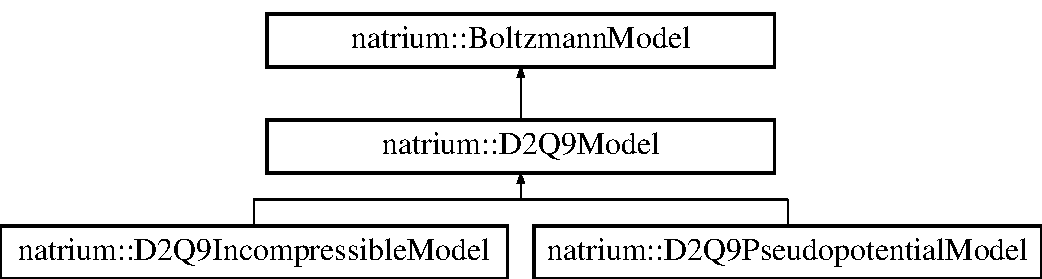
\includegraphics[height=3.000000cm]{classnatrium_1_1D2Q9Model}
\end{center}
\end{figure}
\subsection*{Public Member Functions}
\begin{DoxyCompactItemize}
\item 
\hypertarget{classnatrium_1_1D2Q9Model_af498c14d311e9172d96b5d962ccc5202}{\hyperlink{classnatrium_1_1D2Q9Model_af498c14d311e9172d96b5d962ccc5202}{D2\-Q9\-Model} (double scaling)}\label{classnatrium_1_1D2Q9Model_af498c14d311e9172d96b5d962ccc5202}

\begin{DoxyCompactList}\small\item\em constructor \end{DoxyCompactList}\item 
\hypertarget{classnatrium_1_1D2Q9Model_aec7d8c160f430e14fbede9ecda368797}{virtual \hyperlink{classnatrium_1_1D2Q9Model_aec7d8c160f430e14fbede9ecda368797}{$\sim$\-D2\-Q9\-Model} ()}\label{classnatrium_1_1D2Q9Model_aec7d8c160f430e14fbede9ecda368797}

\begin{DoxyCompactList}\small\item\em destructor \end{DoxyCompactList}\item 
\hypertarget{classnatrium_1_1D2Q9Model_ac9b53eb73e84ecd13afcf9f3a0b0e195}{virtual double {\bfseries get\-Speed\-Of\-Sound} () const }\label{classnatrium_1_1D2Q9Model_ac9b53eb73e84ecd13afcf9f3a0b0e195}

\item 
\hypertarget{classnatrium_1_1D2Q9Model_aa83e54b682ec7081c298324ee9688a8e}{virtual double {\bfseries get\-Speed\-Of\-Sound\-Square} () const }\label{classnatrium_1_1D2Q9Model_aa83e54b682ec7081c298324ee9688a8e}

\item 
\hypertarget{classnatrium_1_1D2Q9Model_ae29e3df458e24802467ca9c2209cc0ca}{virtual size\-\_\-t {\bfseries get\-Index\-Of\-Opposite\-Direction} (size\-\_\-t index) const }\label{classnatrium_1_1D2Q9Model_ae29e3df458e24802467ca9c2209cc0ca}

\end{DoxyCompactItemize}
\subsection*{Static Public Attributes}
\begin{DoxyCompactItemize}
\item 
\hypertarget{classnatrium_1_1D2Q9Model_a81532a1067ba5f280698a1a84711ede5}{static const size\-\_\-t \hyperlink{classnatrium_1_1D2Q9Model_a81532a1067ba5f280698a1a84711ede5}{D} = 2}\label{classnatrium_1_1D2Q9Model_a81532a1067ba5f280698a1a84711ede5}

\begin{DoxyCompactList}\small\item\em D. \end{DoxyCompactList}\item 
\hypertarget{classnatrium_1_1D2Q9Model_ad3d102dfb9c8ad7b56a8f82c3f4286f6}{static const size\-\_\-t \hyperlink{classnatrium_1_1D2Q9Model_ad3d102dfb9c8ad7b56a8f82c3f4286f6}{Q} = 9}\label{classnatrium_1_1D2Q9Model_ad3d102dfb9c8ad7b56a8f82c3f4286f6}

\begin{DoxyCompactList}\small\item\em Q. \end{DoxyCompactList}\end{DoxyCompactItemize}
\subsection*{Protected Attributes}
\begin{DoxyCompactItemize}
\item 
\hypertarget{classnatrium_1_1D2Q9Model_ab212c0c04921591f16c1970d93878cf9}{const double \hyperlink{classnatrium_1_1D2Q9Model_ab212c0c04921591f16c1970d93878cf9}{m\-\_\-speed\-Of\-Sound}}\label{classnatrium_1_1D2Q9Model_ab212c0c04921591f16c1970d93878cf9}

\begin{DoxyCompactList}\small\item\em speed of sound \end{DoxyCompactList}\item 
\hypertarget{classnatrium_1_1D2Q9Model_afa28316438de5055d51674d89a0075ba}{const double \hyperlink{classnatrium_1_1D2Q9Model_afa28316438de5055d51674d89a0075ba}{m\-\_\-speed\-Of\-Sound\-Square}}\label{classnatrium_1_1D2Q9Model_afa28316438de5055d51674d89a0075ba}

\begin{DoxyCompactList}\small\item\em (speed of sound)$^\wedge$2 \end{DoxyCompactList}\end{DoxyCompactItemize}


\subsection{Detailed Description}
D2\-Q9 Model. 

The documentation for this class was generated from the following files\-:\begin{DoxyCompactItemize}
\item 
/home/kraemer/eclipse\-\_\-workspace/\-N\-A\-Triu\-M/src/natrium/boltzmannmodels/\hyperlink{D2Q9Model_8h}{D2\-Q9\-Model.\-h}\item 
/home/kraemer/eclipse\-\_\-workspace/\-N\-A\-Triu\-M/src/natrium/boltzmannmodels/\hyperlink{D2Q9Model_8cpp}{D2\-Q9\-Model.\-cpp}\end{DoxyCompactItemize}

\hypertarget{classnatrium_1_1D2Q9PseudopotentialModel}{\section{natrium\-:\-:D2\-Q9\-Pseudopotential\-Model Class Reference}
\label{classnatrium_1_1D2Q9PseudopotentialModel}\index{natrium\-::\-D2\-Q9\-Pseudopotential\-Model@{natrium\-::\-D2\-Q9\-Pseudopotential\-Model}}
}
Inheritance diagram for natrium\-:\-:D2\-Q9\-Pseudopotential\-Model\-:\begin{figure}[H]
\begin{center}
\leavevmode
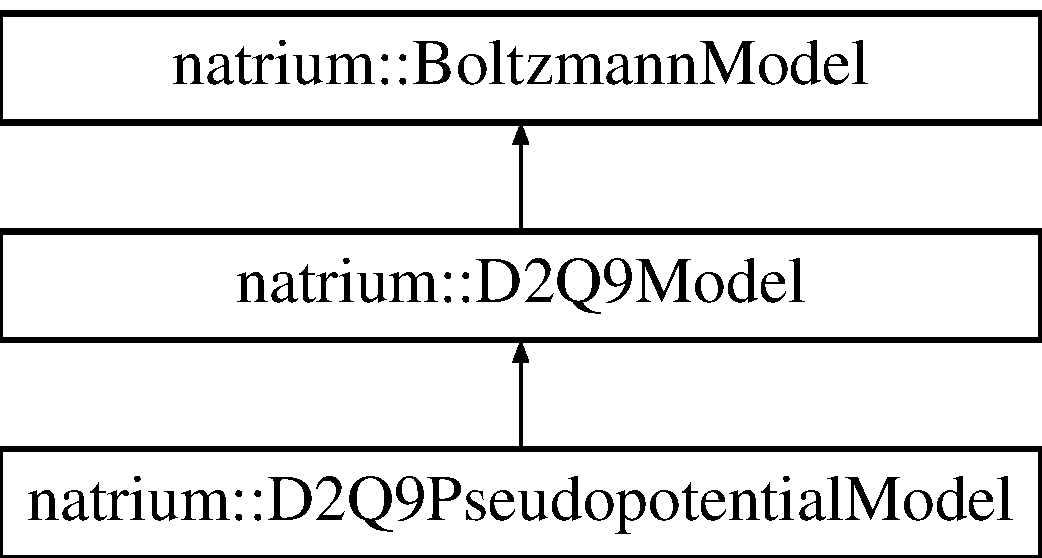
\includegraphics[height=3.000000cm]{classnatrium_1_1D2Q9PseudopotentialModel}
\end{center}
\end{figure}
\subsection*{Public Member Functions}
\begin{DoxyCompactItemize}
\item 
\hypertarget{classnatrium_1_1D2Q9PseudopotentialModel_af533d01219626d11d9f2cf296aa7cc63}{\hyperlink{classnatrium_1_1D2Q9PseudopotentialModel_af533d01219626d11d9f2cf296aa7cc63}{D2\-Q9\-Pseudopotential\-Model} (double scaling, const double dt)}\label{classnatrium_1_1D2Q9PseudopotentialModel_af533d01219626d11d9f2cf296aa7cc63}

\begin{DoxyCompactList}\small\item\em constructor \end{DoxyCompactList}\item 
\hypertarget{classnatrium_1_1D2Q9PseudopotentialModel_ac8cdc8eb6e099490819423455325ecbb}{virtual \hyperlink{classnatrium_1_1D2Q9PseudopotentialModel_ac8cdc8eb6e099490819423455325ecbb}{$\sim$\-D2\-Q9\-Pseudopotential\-Model} ()}\label{classnatrium_1_1D2Q9PseudopotentialModel_ac8cdc8eb6e099490819423455325ecbb}

\begin{DoxyCompactList}\small\item\em destructor \end{DoxyCompactList}\item 
virtual double \hyperlink{classnatrium_1_1D2Q9PseudopotentialModel_a54a15a3c9590e7c40b4b3052fcb7319e}{get\-Equilibrium\-Distribution} (size\-\_\-t i, const numeric\-\_\-vector \&u, const double rho=1) const 
\begin{DoxyCompactList}\small\item\em virtual function for the calculation of the equilibrium distribution \end{DoxyCompactList}\item 
\hypertarget{classnatrium_1_1D2Q9PseudopotentialModel_aa74c0b3299f15d9830cf427b4d61bd68}{void {\bfseries get\-Interaction\-Force} (const vector$<$ double $>$ \&distributions, numeric\-\_\-vector \&interaction\-Force, const double rho=1)}\label{classnatrium_1_1D2Q9PseudopotentialModel_aa74c0b3299f15d9830cf427b4d61bd68}

\item 
\hypertarget{classnatrium_1_1D2Q9PseudopotentialModel_ae8ac734b4cfb98151ed7daa8a9af3af2}{const shared\-\_\-ptr$<$ \hyperlink{classnatrium_1_1SEDGMinLee}{S\-E\-D\-G\-Min\-Lee}$<$ 2 $>$ $>$ {\bfseries get\-Advection\-Operator} () const }\label{classnatrium_1_1D2Q9PseudopotentialModel_ae8ac734b4cfb98151ed7daa8a9af3af2}

\item 
\hypertarget{classnatrium_1_1D2Q9PseudopotentialModel_a192ab3089f17ae9cb95557e03a6a5eaf}{void {\bfseries set\-Advection\-Operator} (const shared\-\_\-ptr$<$ \hyperlink{classnatrium_1_1SEDGMinLee}{S\-E\-D\-G\-Min\-Lee}$<$ 2 $>$ $>$ \&advection\-Operator)}\label{classnatrium_1_1D2Q9PseudopotentialModel_a192ab3089f17ae9cb95557e03a6a5eaf}

\end{DoxyCompactItemize}
\subsection*{Additional Inherited Members}


\subsection{Member Function Documentation}
\hypertarget{classnatrium_1_1D2Q9PseudopotentialModel_a54a15a3c9590e7c40b4b3052fcb7319e}{\index{natrium\-::\-D2\-Q9\-Pseudopotential\-Model@{natrium\-::\-D2\-Q9\-Pseudopotential\-Model}!get\-Equilibrium\-Distribution@{get\-Equilibrium\-Distribution}}
\index{get\-Equilibrium\-Distribution@{get\-Equilibrium\-Distribution}!natrium::D2Q9PseudopotentialModel@{natrium\-::\-D2\-Q9\-Pseudopotential\-Model}}
\subsubsection[{get\-Equilibrium\-Distribution}]{\setlength{\rightskip}{0pt plus 5cm}double natrium\-::\-D2\-Q9\-Pseudopotential\-Model\-::get\-Equilibrium\-Distribution (
\begin{DoxyParamCaption}
\item[{size\-\_\-t}]{i, }
\item[{const numeric\-\_\-vector \&}]{u, }
\item[{const double}]{rho = {\ttfamily 1}}
\end{DoxyParamCaption}
) const\hspace{0.3cm}{\ttfamily [virtual]}}}\label{classnatrium_1_1D2Q9PseudopotentialModel_a54a15a3c9590e7c40b4b3052fcb7319e}


virtual function for the calculation of the equilibrium distribution 


\begin{DoxyParams}{Parameters}
{\em i} & index of the direction \\
\hline
{\em u} & macroscopic velocity \\
\hline
{\em rho} & macroscopic density \\
\hline
\end{DoxyParams}
\begin{DoxyReturn}{Returns}
value of the equilibrium distribution 
\end{DoxyReturn}
\begin{DoxyNote}{Note}
The calculation can surely be done more efficiently by passing different arguments, e.\-g. u$\ast$u or u/(c$^\wedge$2) 
\end{DoxyNote}


Implements \hyperlink{classnatrium_1_1BoltzmannModel_ad482e26c4df3014e4b1447ee6cbb44ff}{natrium\-::\-Boltzmann\-Model}.



The documentation for this class was generated from the following files\-:\begin{DoxyCompactItemize}
\item 
/home/kraemer/eclipse\-\_\-workspace/\-N\-A\-Triu\-M/src/natrium/boltzmannmodels/D2\-Q9\-Pseudopotential\-Model.\-h\item 
/home/kraemer/eclipse\-\_\-workspace/\-N\-A\-Triu\-M/src/natrium/boltzmannmodels/D2\-Q9\-Pseudopotential\-Model.\-cpp\end{DoxyCompactItemize}

\hypertarget{classnatrium_1_1DensityFluctuation2D}{
\section{natrium::DensityFluctuation2D Class Reference}
\label{classnatrium_1_1DensityFluctuation2D}\index{natrium::DensityFluctuation2D@{natrium::DensityFluctuation2D}}
}
Inheritance diagram for natrium::DensityFluctuation2D::\begin{figure}[H]
\begin{center}
\leavevmode
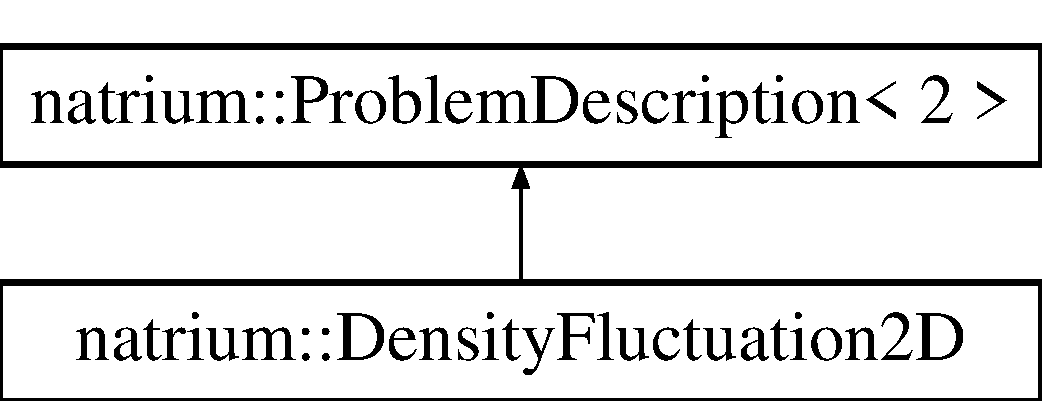
\includegraphics[height=2cm]{classnatrium_1_1DensityFluctuation2D}
\end{center}
\end{figure}
\subsection*{Public Member Functions}
\begin{DoxyCompactItemize}
\item 
\hypertarget{classnatrium_1_1DensityFluctuation2D_aac8ea303ea740e73868cd1ee431e182f}{
{\bfseries DensityFluctuation2D} (double viscosity, size\_\-t refinementLevel)}
\label{classnatrium_1_1DensityFluctuation2D_aac8ea303ea740e73868cd1ee431e182f}

\item 
\hypertarget{classnatrium_1_1DensityFluctuation2D_a7d345499b56b65e0b107defcd5c89e2e}{
virtual void {\bfseries applyInitialDensities} (\hyperlink{namespacenatrium_a903d2b92917f582f2ff05f52160ab811}{distributed\_\-vector} \&initialDensities, const vector$<$ dealii::Point$<$ 2 $>$ $>$ \&supportPoints) const }
\label{classnatrium_1_1DensityFluctuation2D_a7d345499b56b65e0b107defcd5c89e2e}

\item 
\hypertarget{classnatrium_1_1DensityFluctuation2D_a217a8d3635da81fb0350671a86142b57}{
virtual void {\bfseries applyInitialVelocities} (vector$<$ \hyperlink{namespacenatrium_a903d2b92917f582f2ff05f52160ab811}{distributed\_\-vector} $>$ \&initialVelocities, const vector$<$ dealii::Point$<$ 2 $>$ $>$ \&supportPoints) const }
\label{classnatrium_1_1DensityFluctuation2D_a217a8d3635da81fb0350671a86142b57}

\item 
\hypertarget{classnatrium_1_1DensityFluctuation2D_af158622965391ef1c856587d9fb993b7}{
virtual void {\bfseries refine} (Mesh$<$ 2 $>$ \&mesh)}
\label{classnatrium_1_1DensityFluctuation2D_af158622965391ef1c856587d9fb993b7}

\item 
\hypertarget{classnatrium_1_1DensityFluctuation2D_a7b7215ba2073404b076a517ffe2c34ea}{
virtual void {\bfseries transform} (Mesh$<$ 2 $>$ \&mesh)}
\label{classnatrium_1_1DensityFluctuation2D_a7b7215ba2073404b076a517ffe2c34ea}

\end{DoxyCompactItemize}


The documentation for this class was generated from the following files:\begin{DoxyCompactItemize}
\item 
/mnt/fdrive/akraem3m/workspace/NATriuM/src/examples/step-\/99/DensityFluctuation2D.h\item 
/mnt/fdrive/akraem3m/workspace/NATriuM/src/examples/step-\/99/DensityFluctuation2D.cpp\end{DoxyCompactItemize}

\hypertarget{classnatrium_1_1DistributionFunctions}{\section{natrium\-:\-:Distribution\-Functions Class Reference}
\label{classnatrium_1_1DistributionFunctions}\index{natrium\-::\-Distribution\-Functions@{natrium\-::\-Distribution\-Functions}}
}


This class contains the distribution functions. As the zero-\/velocity particles (f0) can be ignored for streaming, f0 is split from the other distribution functions (f\-Stream) in the implementation. f\-Stream is a block vector, which has the advantage that it can be multiplied with the System\-Matrix. The \hyperlink{classnatrium_1_1DistributionFunctions}{Distribution\-Functions} class is designed to mime the behaviour of a vector$<$distributed\-\_\-vector$>$ .  




{\ttfamily \#include $<$Distribution\-Functions.\-h$>$}

\subsection*{Public Member Functions}
\begin{DoxyCompactItemize}
\item 
\hypertarget{classnatrium_1_1DistributionFunctions_a4fc9c42637465355a9df7681d45340c9}{\hyperlink{classnatrium_1_1DistributionFunctions_a4fc9c42637465355a9df7681d45340c9}{Distribution\-Functions} ()}\label{classnatrium_1_1DistributionFunctions_a4fc9c42637465355a9df7681d45340c9}

\begin{DoxyCompactList}\small\item\em empty constructor. Construction is done through reinit. \end{DoxyCompactList}\item 
\hypertarget{classnatrium_1_1DistributionFunctions_af0a970355419acf79be898e573f3149a}{\hyperlink{classnatrium_1_1DistributionFunctions_af0a970355419acf79be898e573f3149a}{Distribution\-Functions} (const \hyperlink{classnatrium_1_1DistributionFunctions}{Distribution\-Functions} \&f)}\label{classnatrium_1_1DistributionFunctions_af0a970355419acf79be898e573f3149a}

\begin{DoxyCompactList}\small\item\em Copy constructor. \end{DoxyCompactList}\item 
\hypertarget{classnatrium_1_1DistributionFunctions_a0ea3ad0426df18a986578f7b57361dd3}{\hyperlink{classnatrium_1_1DistributionFunctions_a0ea3ad0426df18a986578f7b57361dd3}{Distribution\-Functions} (const vector$<$ distributed\-\_\-vector $>$ \&f)}\label{classnatrium_1_1DistributionFunctions_a0ea3ad0426df18a986578f7b57361dd3}

\begin{DoxyCompactList}\small\item\em Copy constructor. Conversion from vector$<$distributed\-\_\-vector$>$. \end{DoxyCompactList}\item 
\hypertarget{classnatrium_1_1DistributionFunctions_af965a46fbf124e8f90250c843e615bcd}{virtual \hyperlink{classnatrium_1_1DistributionFunctions_af965a46fbf124e8f90250c843e615bcd}{$\sim$\-Distribution\-Functions} ()}\label{classnatrium_1_1DistributionFunctions_af965a46fbf124e8f90250c843e615bcd}

\begin{DoxyCompactList}\small\item\em Destructor. \end{DoxyCompactList}\item 
\hypertarget{classnatrium_1_1DistributionFunctions_a34f0147178c17597eaf24befdcced975}{distributed\-\_\-vector \& \hyperlink{classnatrium_1_1DistributionFunctions_a34f0147178c17597eaf24befdcced975}{at} (size\-\_\-t i)}\label{classnatrium_1_1DistributionFunctions_a34f0147178c17597eaf24befdcced975}

\begin{DoxyCompactList}\small\item\em mimes std\-::vector.\-at(i) \end{DoxyCompactList}\item 
\hypertarget{classnatrium_1_1DistributionFunctions_a750d7de21f207ac694c72b215ba7b6de}{const distributed\-\_\-vector \& \hyperlink{classnatrium_1_1DistributionFunctions_a750d7de21f207ac694c72b215ba7b6de}{at} (size\-\_\-t i) const }\label{classnatrium_1_1DistributionFunctions_a750d7de21f207ac694c72b215ba7b6de}

\begin{DoxyCompactList}\small\item\em mimes std\-::vector.\-at(i) \end{DoxyCompactList}\item 
\hypertarget{classnatrium_1_1DistributionFunctions_a3d76ae4f928f324ec82099dbdce678d7}{const distributed\-\_\-vector \& \hyperlink{classnatrium_1_1DistributionFunctions_a3d76ae4f928f324ec82099dbdce678d7}{get\-F0} () const }\label{classnatrium_1_1DistributionFunctions_a3d76ae4f928f324ec82099dbdce678d7}

\begin{DoxyCompactList}\small\item\em F0 denotes the vector $ f_0 $ (zero-\/velocity particles) \end{DoxyCompactList}\item 
\hypertarget{classnatrium_1_1DistributionFunctions_abb98df52461532f58e77741dd9b6a975}{distributed\-\_\-vector \& \hyperlink{classnatrium_1_1DistributionFunctions_abb98df52461532f58e77741dd9b6a975}{get\-F0} ()}\label{classnatrium_1_1DistributionFunctions_abb98df52461532f58e77741dd9b6a975}

\begin{DoxyCompactList}\small\item\em F0 denotes the vector $ f_0 $ (zero-\/velocity particles) \end{DoxyCompactList}\item 
\hypertarget{classnatrium_1_1DistributionFunctions_ae7cc68f9576384b3fbec8f171856f607}{void \hyperlink{classnatrium_1_1DistributionFunctions_ae7cc68f9576384b3fbec8f171856f607}{set\-F0} (const distributed\-\_\-vector \&f0)}\label{classnatrium_1_1DistributionFunctions_ae7cc68f9576384b3fbec8f171856f607}

\begin{DoxyCompactList}\small\item\em F0 denotes the vector $ f_0 $ (zero-\/velocity particles) \end{DoxyCompactList}\item 
\hypertarget{classnatrium_1_1DistributionFunctions_a74dfe8e6ac6d5f463dcb8220f37800a3}{distributed\-\_\-block\-\_\-vector \& \hyperlink{classnatrium_1_1DistributionFunctions_a74dfe8e6ac6d5f463dcb8220f37800a3}{get\-F\-Stream} ()}\label{classnatrium_1_1DistributionFunctions_a74dfe8e6ac6d5f463dcb8220f37800a3}

\begin{DoxyCompactList}\small\item\em F\-Stream denotes the block vector containing the vectors $ f_1, ..., f_Q $. \end{DoxyCompactList}\item 
\hypertarget{classnatrium_1_1DistributionFunctions_a88224d528262c522ea2ad8bec11178c1}{const distributed\-\_\-block\-\_\-vector \& \hyperlink{classnatrium_1_1DistributionFunctions_a88224d528262c522ea2ad8bec11178c1}{get\-F\-Stream} () const }\label{classnatrium_1_1DistributionFunctions_a88224d528262c522ea2ad8bec11178c1}

\begin{DoxyCompactList}\small\item\em F\-Stream denotes the block vector containing the vectors $ f_1, ..., f_Q $. \end{DoxyCompactList}\item 
\hypertarget{classnatrium_1_1DistributionFunctions_ad0ada0c54968a61f78eb1b82eb6c5a68}{void \hyperlink{classnatrium_1_1DistributionFunctions_ad0ada0c54968a61f78eb1b82eb6c5a68}{set\-F\-Stream} (const distributed\-\_\-block\-\_\-vector \&f\-Stream)}\label{classnatrium_1_1DistributionFunctions_ad0ada0c54968a61f78eb1b82eb6c5a68}

\begin{DoxyCompactList}\small\item\em F\-Stream denotes the block vector containing the vectors $ f_1, ..., f_Q $. \end{DoxyCompactList}\item 
\hypertarget{classnatrium_1_1DistributionFunctions_ae0fd8e8234c7d5abec8522767d2a95e7}{const size\-\_\-t \hyperlink{classnatrium_1_1DistributionFunctions_ae0fd8e8234c7d5abec8522767d2a95e7}{get\-Q} () const }\label{classnatrium_1_1DistributionFunctions_ae0fd8e8234c7d5abec8522767d2a95e7}

\begin{DoxyCompactList}\small\item\em the number of discrete velocities \end{DoxyCompactList}\item 
\hypertarget{classnatrium_1_1DistributionFunctions_acaca68f7cbb9322d354ad6dca68b2cb2}{void \hyperlink{classnatrium_1_1DistributionFunctions_acaca68f7cbb9322d354ad6dca68b2cb2}{reinit} (size\-\_\-t Q, size\-\_\-t \hyperlink{classnatrium_1_1DistributionFunctions_a636814c639143c76989b09b2a92b6757}{size})}\label{classnatrium_1_1DistributionFunctions_acaca68f7cbb9322d354ad6dca68b2cb2}

\begin{DoxyCompactList}\small\item\em reinitialize the sizes of the distribution functions \end{DoxyCompactList}\item 
\hypertarget{classnatrium_1_1DistributionFunctions_a636814c639143c76989b09b2a92b6757}{size\-\_\-t \hyperlink{classnatrium_1_1DistributionFunctions_a636814c639143c76989b09b2a92b6757}{size} () const }\label{classnatrium_1_1DistributionFunctions_a636814c639143c76989b09b2a92b6757}

\begin{DoxyCompactList}\small\item\em the number of discrete velocities, including zero \end{DoxyCompactList}\end{DoxyCompactItemize}


\subsection{Detailed Description}
This class contains the distribution functions. As the zero-\/velocity particles (f0) can be ignored for streaming, f0 is split from the other distribution functions (f\-Stream) in the implementation. f\-Stream is a block vector, which has the advantage that it can be multiplied with the System\-Matrix. The \hyperlink{classnatrium_1_1DistributionFunctions}{Distribution\-Functions} class is designed to mime the behaviour of a vector$<$distributed\-\_\-vector$>$ . 

The documentation for this class was generated from the following file\-:\begin{DoxyCompactItemize}
\item 
/home/kraemer/eclipse\-\_\-workspace/\-N\-A\-Triu\-M/src/natrium/solver/Distribution\-Functions.\-h\end{DoxyCompactItemize}

\hypertarget{classnatrium_1_1ErrorStats}{
\section{natrium::ErrorStats$<$ dim $>$ Class Template Reference}
\label{classnatrium_1_1ErrorStats}\index{natrium::ErrorStats@{natrium::ErrorStats}}
}


Container for error statistics and table file; only for use with \hyperlink{classnatrium_1_1BenchmarkCFDSolver}{BenchmarkCFDSolver}.  


{\ttfamily \#include $<$ErrorStats.h$>$}\subsection*{Public Member Functions}
\begin{DoxyCompactItemize}
\item 
\hyperlink{classnatrium_1_1ErrorStats_a1dcdc9cb0508c7f64a067efae4134754}{ErrorStats} (\hyperlink{classnatrium_1_1BenchmarkCFDSolver}{BenchmarkCFDSolver}$<$ dim $>$ $\ast$cfdsolver, const std::string tableFileName=\char`\"{}\char`\"{})
\begin{DoxyCompactList}\small\item\em Constructor. \item\end{DoxyCompactList}\item 
\hypertarget{classnatrium_1_1ErrorStats_ad8cc77e4ac7a50e030e9a49fe1a5bdba}{
void \hyperlink{classnatrium_1_1ErrorStats_ad8cc77e4ac7a50e030e9a49fe1a5bdba}{printHeaderLine} ()}
\label{classnatrium_1_1ErrorStats_ad8cc77e4ac7a50e030e9a49fe1a5bdba}

\begin{DoxyCompactList}\small\item\em write header line to table file \item\end{DoxyCompactList}\item 
\hypertarget{classnatrium_1_1ErrorStats_af02f31d82efefb482ea4ab3d69642486}{
void \hyperlink{classnatrium_1_1ErrorStats_af02f31d82efefb482ea4ab3d69642486}{printNewLine} ()}
\label{classnatrium_1_1ErrorStats_af02f31d82efefb482ea4ab3d69642486}

\begin{DoxyCompactList}\small\item\em write information of the current iteration to table file \item\end{DoxyCompactList}\item 
\hypertarget{classnatrium_1_1ErrorStats_ad24a8dae524127631e75368a0aac61b5}{
void \hyperlink{classnatrium_1_1ErrorStats_ad24a8dae524127631e75368a0aac61b5}{update} ()}
\label{classnatrium_1_1ErrorStats_ad24a8dae524127631e75368a0aac61b5}

\begin{DoxyCompactList}\small\item\em update errors for the current iteration \item\end{DoxyCompactList}\item 
\hypertarget{classnatrium_1_1ErrorStats_a72dcc0b8b86335a50ee1b324bbed0e61}{
bool \hyperlink{classnatrium_1_1ErrorStats_a72dcc0b8b86335a50ee1b324bbed0e61}{isUpToDate} () const }
\label{classnatrium_1_1ErrorStats_a72dcc0b8b86335a50ee1b324bbed0e61}

\begin{DoxyCompactList}\small\item\em check, if errors are up-\/to-\/date, i.e. have already been calculated in the current iteration \item\end{DoxyCompactList}\item 
\hypertarget{classnatrium_1_1ErrorStats_aebc5c3f92adfee93ece2f97275651e44}{
const shared\_\-ptr$<$ std::fstream $>$ \& {\bfseries getErrorsTableFile} () const }
\label{classnatrium_1_1ErrorStats_aebc5c3f92adfee93ece2f97275651e44}

\item 
\hypertarget{classnatrium_1_1ErrorStats_a341ef071a84aa3a2b78485ce90bca7b2}{
const std::string \& {\bfseries getFilename} () const }
\label{classnatrium_1_1ErrorStats_a341ef071a84aa3a2b78485ce90bca7b2}

\item 
\hypertarget{classnatrium_1_1ErrorStats_ab710182a15d0c548fbc8c3b071dbebd1}{
size\_\-t {\bfseries getIterationNumber} () const }
\label{classnatrium_1_1ErrorStats_ab710182a15d0c548fbc8c3b071dbebd1}

\item 
double \hyperlink{classnatrium_1_1ErrorStats_a66f817c7daaf15724d5d42de4f17a1e8}{getL2DensityError} () const 
\begin{DoxyCompactList}\small\item\em return L2-\/Error of density, $ \sqrt{ \sum_{i=1}^{N} (\rho_{i} - \rho_{i}^{ref})^{2} } $ \item\end{DoxyCompactList}\item 
double \hyperlink{classnatrium_1_1ErrorStats_a201f625a3607a814fdd645aabfe37fbc}{getL2VelocityError} () const 
\begin{DoxyCompactList}\small\item\em return L2-\/Error of velocity, $ \sqrt{ \sum_{i=1}^{N} \|u_{i} - u_{i}^{ref}\|_{2}^{2} } $ \item\end{DoxyCompactList}\item 
\hypertarget{classnatrium_1_1ErrorStats_a8e32b3e8c8d141b6cdcf5428613a875e}{
double \hyperlink{classnatrium_1_1ErrorStats_a8e32b3e8c8d141b6cdcf5428613a875e}{getMaxDensityError} () const }
\label{classnatrium_1_1ErrorStats_a8e32b3e8c8d141b6cdcf5428613a875e}

\begin{DoxyCompactList}\small\item\em return max error of density $ max | \rho_{i} - \rho_{i}^{ref} | $ \item\end{DoxyCompactList}\item 
\hypertarget{classnatrium_1_1ErrorStats_a350f6b6fcc91f18006095331b0aa430c}{
double {\bfseries getMaxUAnalytic} () const }
\label{classnatrium_1_1ErrorStats_a350f6b6fcc91f18006095331b0aa430c}

\item 
\hypertarget{classnatrium_1_1ErrorStats_a48ea1bfc5db4dad6369b4b2991aa1f5c}{
double \hyperlink{classnatrium_1_1ErrorStats_a48ea1bfc5db4dad6369b4b2991aa1f5c}{getMaxVelocityError} () const }
\label{classnatrium_1_1ErrorStats_a48ea1bfc5db4dad6369b4b2991aa1f5c}

\begin{DoxyCompactList}\small\item\em return max error of velocity $ max \|u_{i} - u_{i}^{ref}\|_{2} $ \item\end{DoxyCompactList}\item 
\hypertarget{classnatrium_1_1ErrorStats_aa79b49d872935e567c94a2727af24dea}{
double {\bfseries getTime} () const }
\label{classnatrium_1_1ErrorStats_aa79b49d872935e567c94a2727af24dea}

\item 
\hypertarget{classnatrium_1_1ErrorStats_a965b8a50d1f84d8962c995808c222799}{
double {\bfseries getL2UAnalytic} () const }
\label{classnatrium_1_1ErrorStats_a965b8a50d1f84d8962c995808c222799}

\end{DoxyCompactItemize}


\subsection{Detailed Description}
\subsubsection*{template$<$size\_\-t dim$>$ class natrium::ErrorStats$<$ dim $>$}

Container for error statistics and table file; only for use with \hyperlink{classnatrium_1_1BenchmarkCFDSolver}{BenchmarkCFDSolver}. \begin{DoxyNote}{Note}
As this class is a friend of \hyperlink{classnatrium_1_1BenchmarkCFDSolver}{BenchmarkCFDSolver}, it can access its private attributes 
\end{DoxyNote}


\subsection{Constructor \& Destructor Documentation}
\hypertarget{classnatrium_1_1ErrorStats_a1dcdc9cb0508c7f64a067efae4134754}{
\index{natrium::ErrorStats@{natrium::ErrorStats}!ErrorStats@{ErrorStats}}
\index{ErrorStats@{ErrorStats}!natrium::ErrorStats@{natrium::ErrorStats}}
\subsubsection[{ErrorStats}]{\setlength{\rightskip}{0pt plus 5cm}template$<$size\_\-t dim$>$ {\bf natrium::ErrorStats}$<$ dim $>$::{\bf ErrorStats} ({\bf BenchmarkCFDSolver}$<$ dim $>$ $\ast$ {\em cfdsolver}, \/  const std::string {\em tableFileName} = {\ttfamily \char`\"{}\char`\"{}})\hspace{0.3cm}{\ttfamily  \mbox{[}inline\mbox{]}}}}
\label{classnatrium_1_1ErrorStats_a1dcdc9cb0508c7f64a067efae4134754}


Constructor. 
\begin{DoxyParams}{Parameters}
\item[{\em cfdsolver}]Instance of \hyperlink{classnatrium_1_1CFDSolver}{CFDSolver} object \item[{\em tableFileName}]Default: \char`\"{}\char`\"{} means: switch output off \end{DoxyParams}


\subsection{Member Function Documentation}
\hypertarget{classnatrium_1_1ErrorStats_a66f817c7daaf15724d5d42de4f17a1e8}{
\index{natrium::ErrorStats@{natrium::ErrorStats}!getL2DensityError@{getL2DensityError}}
\index{getL2DensityError@{getL2DensityError}!natrium::ErrorStats@{natrium::ErrorStats}}
\subsubsection[{getL2DensityError}]{\setlength{\rightskip}{0pt plus 5cm}template$<$size\_\-t dim$>$ double {\bf natrium::ErrorStats}$<$ dim $>$::getL2DensityError () const\hspace{0.3cm}{\ttfamily  \mbox{[}inline\mbox{]}}}}
\label{classnatrium_1_1ErrorStats_a66f817c7daaf15724d5d42de4f17a1e8}


return L2-\/Error of density, $ \sqrt{ \sum_{i=1}^{N} (\rho_{i} - \rho_{i}^{ref})^{2} } $ \begin{DoxyNote}{Note}
The division by the number of dofs is required, because otherwise finer grids result in bigger errors. 
\end{DoxyNote}
\hypertarget{classnatrium_1_1ErrorStats_a201f625a3607a814fdd645aabfe37fbc}{
\index{natrium::ErrorStats@{natrium::ErrorStats}!getL2VelocityError@{getL2VelocityError}}
\index{getL2VelocityError@{getL2VelocityError}!natrium::ErrorStats@{natrium::ErrorStats}}
\subsubsection[{getL2VelocityError}]{\setlength{\rightskip}{0pt plus 5cm}template$<$size\_\-t dim$>$ double {\bf natrium::ErrorStats}$<$ dim $>$::getL2VelocityError () const\hspace{0.3cm}{\ttfamily  \mbox{[}inline\mbox{]}}}}
\label{classnatrium_1_1ErrorStats_a201f625a3607a814fdd645aabfe37fbc}


return L2-\/Error of velocity, $ \sqrt{ \sum_{i=1}^{N} \|u_{i} - u_{i}^{ref}\|_{2}^{2} } $ \begin{DoxyNote}{Note}
The division by the number of dofs is required, because otherwise finer grids result in bigger errors. 
\end{DoxyNote}


The documentation for this class was generated from the following files:\begin{DoxyCompactItemize}
\item 
/mnt/fdrive/akraem3m/workspace/NATriuM/src/library/natrium/solver/ErrorStats.h\item 
/mnt/fdrive/akraem3m/workspace/NATriuM/src/library/natrium/solver/ErrorStats.cpp\end{DoxyCompactItemize}

\hypertarget{classnatrium_1_1ExponentialTimeIntegrator}{
\section{natrium::ExponentialTimeIntegrator$<$ MATRIX, VECTOR $>$ Class Template Reference}
\label{classnatrium_1_1ExponentialTimeIntegrator}\index{natrium::ExponentialTimeIntegrator@{natrium::ExponentialTimeIntegrator}}
}


Exponential time integration scheme for the solution of f' = L$\ast$f, as used in Uga etal. (2012) Spectral-\/element discontinuous Galerkin lattice Boltzmann simulation of flow past two cylinders in tandem with an exponential time integrator, CMWA 65 pp. 239-\/251.  


{\ttfamily \#include $<$ExponentialTimeIntegrator.h$>$}Inheritance diagram for natrium::ExponentialTimeIntegrator$<$ MATRIX, VECTOR $>$::\begin{figure}[H]
\begin{center}
\leavevmode
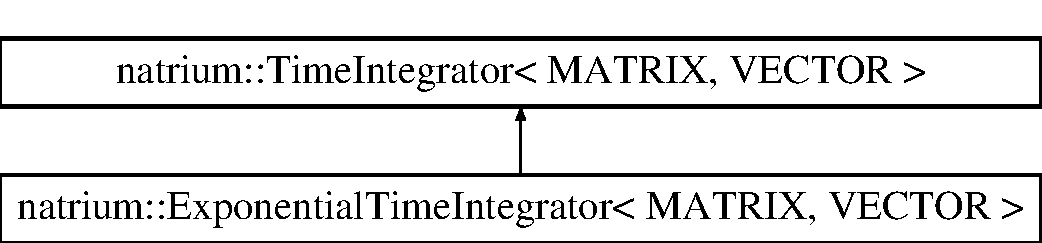
\includegraphics[height=2cm]{classnatrium_1_1ExponentialTimeIntegrator}
\end{center}
\end{figure}
\subsection*{Public Member Functions}
\begin{DoxyCompactItemize}
\item 
\hypertarget{classnatrium_1_1ExponentialTimeIntegrator_a3a3e7b0c53b5c083dbdb7b3d625d8087}{
\hyperlink{classnatrium_1_1ExponentialTimeIntegrator_a3a3e7b0c53b5c083dbdb7b3d625d8087}{ExponentialTimeIntegrator} (double timeStepSize)}
\label{classnatrium_1_1ExponentialTimeIntegrator_a3a3e7b0c53b5c083dbdb7b3d625d8087}

\begin{DoxyCompactList}\small\item\em constructor \item\end{DoxyCompactList}\item 
\hypertarget{classnatrium_1_1ExponentialTimeIntegrator_a7da2892aead7c5e1fec82be549dcb37b}{
{\bfseries ExponentialTimeIntegrator} (double timeStepSize, size\_\-t numberOfBlocks)}
\label{classnatrium_1_1ExponentialTimeIntegrator_a7da2892aead7c5e1fec82be549dcb37b}

\item 
\hypertarget{classnatrium_1_1ExponentialTimeIntegrator_ad85e62117ec3dbfebfbccd6ad1135d8c}{
virtual \hyperlink{classnatrium_1_1ExponentialTimeIntegrator_ad85e62117ec3dbfebfbccd6ad1135d8c}{$\sim$ExponentialTimeIntegrator} ()}
\label{classnatrium_1_1ExponentialTimeIntegrator_ad85e62117ec3dbfebfbccd6ad1135d8c}

\begin{DoxyCompactList}\small\item\em destructor \item\end{DoxyCompactList}\item 
virtual double \hyperlink{classnatrium_1_1ExponentialTimeIntegrator_ae0a9cff9bdafab123016db72d1439ef8}{step} (VECTOR \&f, const MATRIX \&systemMatrix, const VECTOR \&systemVector, double t=0, double dt=0)
\begin{DoxyCompactList}\small\item\em make one time integration step on f: \[ \frac{df}{dt} = Af+b \]. \item\end{DoxyCompactList}\item 
\hypertarget{classnatrium_1_1ExponentialTimeIntegrator_a7b68727897acae02ff025c39a56a4bf6}{
{\footnotesize template$<$$>$ }\\{\bfseries ExponentialTimeIntegrator} (double timeStepSize)}
\label{classnatrium_1_1ExponentialTimeIntegrator_a7b68727897acae02ff025c39a56a4bf6}

\item 
\hypertarget{classnatrium_1_1ExponentialTimeIntegrator_acbd606f38f9c5c0b4cb9b9fc817f1186}{
{\footnotesize template$<$$>$ }\\{\bfseries ExponentialTimeIntegrator} (double timeStepSize, size\_\-t)}
\label{classnatrium_1_1ExponentialTimeIntegrator_acbd606f38f9c5c0b4cb9b9fc817f1186}

\item 
\hypertarget{classnatrium_1_1ExponentialTimeIntegrator_a9fbf0f44e2d68eab2df6d767e6f08c77}{
{\footnotesize template$<$$>$ }\\{\bfseries ExponentialTimeIntegrator} (double timeStepSize)}
\label{classnatrium_1_1ExponentialTimeIntegrator_a9fbf0f44e2d68eab2df6d767e6f08c77}

\item 
\hypertarget{classnatrium_1_1ExponentialTimeIntegrator_a716b2f09970240253c9175e3ad5e3965}{
{\footnotesize template$<$$>$ }\\{\bfseries ExponentialTimeIntegrator} (double timeStepSize, size\_\-t)}
\label{classnatrium_1_1ExponentialTimeIntegrator_a716b2f09970240253c9175e3ad5e3965}

\item 
\hypertarget{classnatrium_1_1ExponentialTimeIntegrator_a04d6a47d38318ab92ba4bd22b834d6c3}{
{\footnotesize template$<$$>$ }\\dealii::IndexSet {\bfseries getIndexSet} (const distributed\_\-sparse\_\-matrix \&m)}
\label{classnatrium_1_1ExponentialTimeIntegrator_a04d6a47d38318ab92ba4bd22b834d6c3}

\item 
\hypertarget{classnatrium_1_1ExponentialTimeIntegrator_aa58b4f252c2f19808f10102d60eed3a9}{
{\footnotesize template$<$$>$ }\\dealii::IndexSet {\bfseries getIndexSet} (const distributed\_\-sparse\_\-block\_\-matrix \&m)}
\label{classnatrium_1_1ExponentialTimeIntegrator_aa58b4f252c2f19808f10102d60eed3a9}

\item 
\hypertarget{classnatrium_1_1ExponentialTimeIntegrator_a6ea6d696834a57e0e8af03558ffc1d5b}{
{\footnotesize template$<$$>$ }\\dealii::IndexSet {\bfseries getIndexSet} (const sparse\_\-matrix \&m)}
\label{classnatrium_1_1ExponentialTimeIntegrator_a6ea6d696834a57e0e8af03558ffc1d5b}

\item 
\hypertarget{classnatrium_1_1ExponentialTimeIntegrator_a0d43b0a3b92ced2b9b7755549742baa0}{
{\footnotesize template$<$$>$ }\\dealii::IndexSet {\bfseries getIndexSet} (const sparse\_\-block\_\-matrix \&m)}
\label{classnatrium_1_1ExponentialTimeIntegrator_a0d43b0a3b92ced2b9b7755549742baa0}

\end{DoxyCompactItemize}


\subsection{Detailed Description}
\subsubsection*{template$<$class MATRIX, class VECTOR$>$ class natrium::ExponentialTimeIntegrator$<$ MATRIX, VECTOR $>$}

Exponential time integration scheme for the solution of f' = L$\ast$f, as used in Uga etal. (2012) Spectral-\/element discontinuous Galerkin lattice Boltzmann simulation of flow past two cylinders in tandem with an exponential time integrator, CMWA 65 pp. 239-\/251. 

\subsection{Member Function Documentation}
\hypertarget{classnatrium_1_1ExponentialTimeIntegrator_ae0a9cff9bdafab123016db72d1439ef8}{
\index{natrium::ExponentialTimeIntegrator@{natrium::ExponentialTimeIntegrator}!step@{step}}
\index{step@{step}!natrium::ExponentialTimeIntegrator@{natrium::ExponentialTimeIntegrator}}
\subsubsection[{step}]{\setlength{\rightskip}{0pt plus 5cm}template$<$class MATRIX , class VECTOR $>$ double {\bf natrium::ExponentialTimeIntegrator}$<$ MATRIX, VECTOR $>$::step (VECTOR \& {\em f}, \/  const MATRIX \& {\em systemMatrix}, \/  const VECTOR \& {\em systemVector}, \/  double {\em t} = {\ttfamily 0}, \/  double {\em dt} = {\ttfamily 0})\hspace{0.3cm}{\ttfamily  \mbox{[}inline, virtual\mbox{]}}}}
\label{classnatrium_1_1ExponentialTimeIntegrator_ae0a9cff9bdafab123016db72d1439ef8}


make one time integration step on f: \[ \frac{df}{dt} = Af+b \]. 
\begin{DoxyParams}{Parameters}
\item[{\em in/out\mbox{]}}]f Vector of degrees of freedom \item[\mbox{$\leftarrow$} {\em systemMatrix}]Matrix A \item[\mbox{$\leftarrow$} {\em systemVector}]Vector b \item[\mbox{$\leftarrow$} {\em double}]t global time \item[\mbox{$\leftarrow$} {\em double}]dt time step size. Required to interface deal.II's embedded RK methods \end{DoxyParams}
\begin{DoxyReturn}{Returns}
new global time 
\end{DoxyReturn}
\begin{DoxyNote}{Note}
fully virtual method. Overloaded by subclasses. 
\end{DoxyNote}


Implements \hyperlink{classnatrium_1_1TimeIntegrator_a1c438e41d183d172d524aa5dc97785fb}{natrium::TimeIntegrator$<$ MATRIX, VECTOR $>$}.

The documentation for this class was generated from the following files:\begin{DoxyCompactItemize}
\item 
/mnt/fdrive/akraem3m/workspace/NATriuM/src/library/natrium/timeintegration/ExponentialTimeIntegrator.h\item 
/mnt/fdrive/akraem3m/workspace/NATriuM/src/library/natrium/timeintegration/\hyperlink{ExponentialTimeIntegrator_8cpp}{ExponentialTimeIntegrator.cpp}\end{DoxyCompactItemize}

\hypertarget{classHtmlTrace}{
\section{HtmlTrace Class Reference}
\label{classHtmlTrace}\index{HtmlTrace@{HtmlTrace}}
}


Stream integration test results to a html file.  


{\ttfamily \#include $<$HtmlTrace.h$>$}\subsection*{Public Member Functions}
\begin{DoxyCompactItemize}
\item 
\hypertarget{classHtmlTrace_aad24986d7bce81d050ea6f5ec4773be7}{
\hyperlink{classHtmlTrace_aad24986d7bce81d050ea6f5ec4773be7}{HtmlTrace} ()}
\label{classHtmlTrace_aad24986d7bce81d050ea6f5ec4773be7}

\begin{DoxyCompactList}\small\item\em Constructor. \item\end{DoxyCompactList}\item 
\hypertarget{classHtmlTrace_a27003513f2782cbd57bf387a1fca8be5}{
\hyperlink{classHtmlTrace_a27003513f2782cbd57bf387a1fca8be5}{$\sim$HtmlTrace} ()}
\label{classHtmlTrace_a27003513f2782cbd57bf387a1fca8be5}

\begin{DoxyCompactList}\small\item\em Destructor. \item\end{DoxyCompactList}\item 
\hypertarget{classHtmlTrace_a334a99ca80288f4b25ee6e5d02edf679}{
std::ofstream \& \hyperlink{classHtmlTrace_a334a99ca80288f4b25ee6e5d02edf679}{getHtml} ()}
\label{classHtmlTrace_a334a99ca80288f4b25ee6e5d02edf679}

\begin{DoxyCompactList}\small\item\em Return stream. \item\end{DoxyCompactList}\end{DoxyCompactItemize}


\subsection{Detailed Description}
Stream integration test results to a html file. 

The documentation for this class was generated from the following files:\begin{DoxyCompactItemize}
\item 
/mnt/fdrive/akraem3m/workspace/NATriuM/src/library/natrium/utilities/HtmlTrace.h\item 
/mnt/fdrive/akraem3m/workspace/NATriuM/src/library/natrium/utilities/HtmlTrace.cpp\end{DoxyCompactItemize}

\hypertarget{classnatrium_1_1LidDrivenCavity2D}{
\section{natrium::LidDrivenCavity2D Class Reference}
\label{classnatrium_1_1LidDrivenCavity2D}\index{natrium::LidDrivenCavity2D@{natrium::LidDrivenCavity2D}}
}


Description of a lid-\/driven cavity flow.  


{\ttfamily \#include $<$LidDrivenCavity2D.h$>$}Inheritance diagram for natrium::LidDrivenCavity2D::\begin{figure}[H]
\begin{center}
\leavevmode
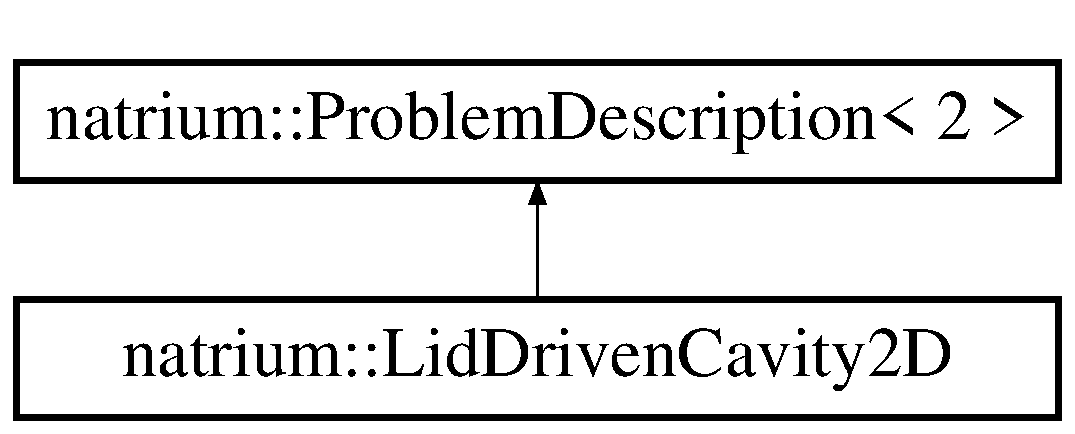
\includegraphics[height=2cm]{classnatrium_1_1LidDrivenCavity2D}
\end{center}
\end{figure}
\subsection*{Classes}
\begin{DoxyCompactItemize}
\item 
struct {\bfseries UnstructuredGridFunc}
\begin{DoxyCompactList}\small\item\em function to generate the unstructured mesh grid \item\end{DoxyCompactList}\end{DoxyCompactItemize}
\subsection*{Public Member Functions}
\begin{DoxyCompactItemize}
\item 
\hyperlink{classnatrium_1_1LidDrivenCavity2D_a139fe700f3e871e1b51eada1a41c69b1}{LidDrivenCavity2D} (double velocity, double viscosity, size\_\-t refinementLevel)
\begin{DoxyCompactList}\small\item\em constructor \item\end{DoxyCompactList}\item 
\hypertarget{classnatrium_1_1LidDrivenCavity2D_a8ae5029b008eb3d3c810bae81440b29c}{
virtual \hyperlink{classnatrium_1_1LidDrivenCavity2D_a8ae5029b008eb3d3c810bae81440b29c}{$\sim$LidDrivenCavity2D} ()}
\label{classnatrium_1_1LidDrivenCavity2D_a8ae5029b008eb3d3c810bae81440b29c}

\begin{DoxyCompactList}\small\item\em destructor \item\end{DoxyCompactList}\item 
\hypertarget{classnatrium_1_1LidDrivenCavity2D_a82c2d453cd5dd83f09a438201a7adec6}{
virtual double {\bfseries getCharacteristicVelocity} () const }
\label{classnatrium_1_1LidDrivenCavity2D_a82c2d453cd5dd83f09a438201a7adec6}

\item 
\hypertarget{classnatrium_1_1LidDrivenCavity2D_a1899d1f52f6f0e25f6be7dff5746efb9}{
virtual void {\bfseries refine} (Mesh$<$ 2 $>$ \&mesh)}
\label{classnatrium_1_1LidDrivenCavity2D_a1899d1f52f6f0e25f6be7dff5746efb9}

\item 
\hypertarget{classnatrium_1_1LidDrivenCavity2D_af42aefb1a7b763f7b0cca834038b5290}{
virtual void {\bfseries transform} (Mesh$<$ 2 $>$ \&mesh)}
\label{classnatrium_1_1LidDrivenCavity2D_af42aefb1a7b763f7b0cca834038b5290}

\end{DoxyCompactItemize}


\subsection{Detailed Description}
Description of a lid-\/driven cavity flow. \begin{Desc}
\item[Examples: ]\par


\hyperlink{step-0_8cpp-example}{step-\/0.cpp}.\end{Desc}


\subsection{Constructor \& Destructor Documentation}
\hypertarget{classnatrium_1_1LidDrivenCavity2D_a139fe700f3e871e1b51eada1a41c69b1}{
\index{natrium::LidDrivenCavity2D@{natrium::LidDrivenCavity2D}!LidDrivenCavity2D@{LidDrivenCavity2D}}
\index{LidDrivenCavity2D@{LidDrivenCavity2D}!natrium::LidDrivenCavity2D@{natrium::LidDrivenCavity2D}}
\subsubsection[{LidDrivenCavity2D}]{\setlength{\rightskip}{0pt plus 5cm}natrium::LidDrivenCavity2D::LidDrivenCavity2D (double {\em velocity}, \/  double {\em viscosity}, \/  size\_\-t {\em refinementLevel})}}
\label{classnatrium_1_1LidDrivenCavity2D_a139fe700f3e871e1b51eada1a41c69b1}


constructor 

apply boundary values 

The documentation for this class was generated from the following files:\begin{DoxyCompactItemize}
\item 
/mnt/fdrive/akraem3m/workspace/NATriuM/src/examples/step-\/0/\hyperlink{LidDrivenCavity2D_8h}{LidDrivenCavity2D.h}\item 
/mnt/fdrive/akraem3m/workspace/NATriuM/src/examples/step-\/0/\hyperlink{LidDrivenCavity2D_8cpp}{LidDrivenCavity2D.cpp}\end{DoxyCompactItemize}

\hypertarget{classnatrium_1_1Logging}{\section{natrium\-:\-:Logging Class Reference}
\label{classnatrium_1_1Logging}\index{natrium\-::\-Logging@{natrium\-::\-Logging}}
}


this class is responsible for output streams to the command line and log file  




{\ttfamily \#include $<$Logging.\-h$>$}

\subsection*{Static Public Attributes}
\begin{DoxyCompactItemize}
\item 
\hypertarget{classnatrium_1_1Logging_a3f7c1686be8b25fcfec6f624467d6346}{static boost\-::shared\-\_\-ptr\\*
$<$ Tee\-Stream $>$ \hyperlink{classnatrium_1_1Logging_a3f7c1686be8b25fcfec6f624467d6346}{F\-U\-L\-L} = boost\-::make\-\_\-shared$<$Tee\-Stream$>$(full\-Tee)}\label{classnatrium_1_1Logging_a3f7c1686be8b25fcfec6f624467d6346}

\begin{DoxyCompactList}\small\item\em Full (complete) log; stream for detailed information. \end{DoxyCompactList}\item 
\hypertarget{classnatrium_1_1Logging_addbf66b690d29a9f8ca9edbc82672d36}{static boost\-::shared\-\_\-ptr\\*
$<$ Tee\-Stream $>$ \hyperlink{classnatrium_1_1Logging_addbf66b690d29a9f8ca9edbc82672d36}{B\-A\-S\-I\-C} = boost\-::make\-\_\-shared$<$Tee\-Stream$>$(basic\-Tee)}\label{classnatrium_1_1Logging_addbf66b690d29a9f8ca9edbc82672d36}

\begin{DoxyCompactList}\small\item\em Stream for basic information. \end{DoxyCompactList}\item 
\hypertarget{classnatrium_1_1Logging_a83b60e3e23cc20425605e3b57962460d}{static boost\-::shared\-\_\-ptr\\*
$<$ Tee\-Stream $>$ \hyperlink{classnatrium_1_1Logging_a83b60e3e23cc20425605e3b57962460d}{E\-R\-R\-O\-R} = boost\-::make\-\_\-shared$<$Tee\-Stream$>$(error\-Tee)}\label{classnatrium_1_1Logging_a83b60e3e23cc20425605e3b57962460d}

\begin{DoxyCompactList}\small\item\em Stream for error messages. \end{DoxyCompactList}\end{DoxyCompactItemize}


\subsection{Detailed Description}
this class is responsible for output streams to the command line and log file 

The documentation for this class was generated from the following files\-:\begin{DoxyCompactItemize}
\item 
/home/kraemer/eclipse\-\_\-workspace/\-N\-A\-Triu\-M/src/natrium/utilities/\hyperlink{Logging_8h}{Logging.\-h}\item 
/home/kraemer/eclipse\-\_\-workspace/\-N\-A\-Triu\-M/src/natrium/utilities/Logging.\-cpp\end{DoxyCompactItemize}

\hypertarget{classnatrium_1_1matrixAnalysis}{\section{natrium\-:\-:matrix\-Analysis$<$ dim $>$ Class Template Reference}
\label{classnatrium_1_1matrixAnalysis}\index{natrium\-::matrix\-Analysis$<$ dim $>$@{natrium\-::matrix\-Analysis$<$ dim $>$}}
}


Calculation of spectra and pseudospectra of streaming matrices.  




{\ttfamily \#include $<$matrix\-Analysis.\-h$>$}

\subsection*{Public Member Functions}
\begin{DoxyCompactItemize}
\item 
\hypertarget{classnatrium_1_1matrixAnalysis_ab1434eb6a7256560cbeaf2f3869709ed}{{\bfseries matrix\-Analysis} (shared\-\_\-ptr$<$ \hyperlink{classnatrium_1_1CFDSolver}{C\-F\-D\-Solver}$<$ dim $>$ $>$ solver)}\label{classnatrium_1_1matrixAnalysis_ab1434eb6a7256560cbeaf2f3869709ed}

\item 
void \hyperlink{classnatrium_1_1matrixAnalysis_af83535a0c1c83db223649b958c245df1}{write\-Spectrum} ()
\begin{DoxyCompactList}\small\item\em Write the spectrum of the \hyperlink{classnatrium_1_1CFDSolver}{C\-F\-D\-Solver}'s streaming matrix to the file spectrum.\-txt in the Output\-Directory. \end{DoxyCompactList}\item 
void \hyperlink{classnatrium_1_1matrixAnalysis_a2c18eb04461c90bfdf3f301e8c9dfc1b}{write\-Pseudospectrum} (size\-\_\-t number\-Of\-Cycles=10, double perturbation=0.\-1)
\begin{DoxyCompactList}\small\item\em Write the pseudospectrum of the \hyperlink{classnatrium_1_1CFDSolver}{C\-F\-D\-Solver}'s streaming matrix to the file pseudospectrum.\-txt in the Output\-Directory. The pseudospectrum contains the eigenvalues of all matrices that are \char`\"{}close to the matrix A\char`\"{}, i.\-e. all entries can be perturbed by a small number. \end{DoxyCompactList}\item 
\hypertarget{classnatrium_1_1matrixAnalysis_af859304140aa0d5e5429bacdd6341d3e}{{\footnotesize template$<$$>$ }\\{\bfseries matrix\-Analysis} (shared\-\_\-ptr$<$ \hyperlink{classnatrium_1_1CFDSolver}{C\-F\-D\-Solver}$<$ 2 $>$ $>$ solver)}\label{classnatrium_1_1matrixAnalysis_af859304140aa0d5e5429bacdd6341d3e}

\item 
\hypertarget{classnatrium_1_1matrixAnalysis_a4ef4d76dd9e24c90a6844edeef6de313}{{\footnotesize template$<$$>$ }\\{\bfseries matrix\-Analysis} (shared\-\_\-ptr$<$ \hyperlink{classnatrium_1_1CFDSolver}{C\-F\-D\-Solver}$<$ 3 $>$ $>$ solver)}\label{classnatrium_1_1matrixAnalysis_a4ef4d76dd9e24c90a6844edeef6de313}

\end{DoxyCompactItemize}
\subsection*{Static Public Member Functions}
\begin{DoxyCompactItemize}
\item 
static void \hyperlink{classnatrium_1_1matrixAnalysis_a78f3d3996a02982e4b465b627a9b999f}{compute\-Spectrum} (const distributed\-\_\-sparse\-\_\-block\-\_\-matrix \&matrix, vector$<$ std\-::complex$<$ double $>$ $>$ \&eigenvalues, double perturbation=0.\-0)
\begin{DoxyCompactList}\small\item\em Compute the eigenvalues of a sparse block matrix. \end{DoxyCompactList}\end{DoxyCompactItemize}


\subsection{Detailed Description}
\subsubsection*{template$<$size\-\_\-t dim$>$class natrium\-::matrix\-Analysis$<$ dim $>$}

Calculation of spectra and pseudospectra of streaming matrices. 

\subsection{Member Function Documentation}
\hypertarget{classnatrium_1_1matrixAnalysis_a78f3d3996a02982e4b465b627a9b999f}{\index{natrium\-::matrix\-Analysis@{natrium\-::matrix\-Analysis}!compute\-Spectrum@{compute\-Spectrum}}
\index{compute\-Spectrum@{compute\-Spectrum}!natrium::matrixAnalysis@{natrium\-::matrix\-Analysis}}
\subsubsection[{compute\-Spectrum}]{\setlength{\rightskip}{0pt plus 5cm}template$<$size\-\_\-t dim$>$ template void {\bf natrium\-::matrix\-Analysis}$<$ dim $>$\-::compute\-Spectrum (
\begin{DoxyParamCaption}
\item[{const distributed\-\_\-sparse\-\_\-block\-\_\-matrix \&}]{matrix, }
\item[{vector$<$ std\-::complex$<$ double $>$ $>$ \&}]{eigenvalues, }
\item[{double}]{perturbation = {\ttfamily 0.0}}
\end{DoxyParamCaption}
)\hspace{0.3cm}{\ttfamily [static]}}}\label{classnatrium_1_1matrixAnalysis_a78f3d3996a02982e4b465b627a9b999f}


Compute the eigenvalues of a sparse block matrix. 


\begin{DoxyParams}{Parameters}
{\em matrix} & the matrix \\
\hline
{\em eigenvalues} & Vector of eigenvalues. Is automatically resized by the method. \\
\hline
{\em perturbation} & Can be used to perturb all matrix entries by a random number in the interval \mbox{[}-\/perturbation, perturbation\mbox{]}. This is required for the calculation of pseudospectra. Default\-: 0.\-0 (no perturbation). \\
\hline
\end{DoxyParams}
\begin{DoxyNote}{Note}
Only practicable for small matrices, as the sparse matrix is turned into a full matrix. 
\end{DoxyNote}
\hypertarget{classnatrium_1_1matrixAnalysis_a2c18eb04461c90bfdf3f301e8c9dfc1b}{\index{natrium\-::matrix\-Analysis@{natrium\-::matrix\-Analysis}!write\-Pseudospectrum@{write\-Pseudospectrum}}
\index{write\-Pseudospectrum@{write\-Pseudospectrum}!natrium::matrixAnalysis@{natrium\-::matrix\-Analysis}}
\subsubsection[{write\-Pseudospectrum}]{\setlength{\rightskip}{0pt plus 5cm}template$<$size\-\_\-t dim$>$ template void {\bf natrium\-::matrix\-Analysis}$<$ dim $>$\-::write\-Pseudospectrum (
\begin{DoxyParamCaption}
\item[{size\-\_\-t}]{number\-Of\-Cycles = {\ttfamily 10}, }
\item[{double}]{perturbation = {\ttfamily 0.1}}
\end{DoxyParamCaption}
)}}\label{classnatrium_1_1matrixAnalysis_a2c18eb04461c90bfdf3f301e8c9dfc1b}


Write the pseudospectrum of the \hyperlink{classnatrium_1_1CFDSolver}{C\-F\-D\-Solver}'s streaming matrix to the file pseudospectrum.\-txt in the Output\-Directory. The pseudospectrum contains the eigenvalues of all matrices that are \char`\"{}close to the matrix A\char`\"{}, i.\-e. all entries can be perturbed by a small number. 


\begin{DoxyParams}{Parameters}
{\em number\-Of\-Cycles} & The number of matrices \char`\"{}close to A\char`\"{}, whose eigenvalues will be calculated. Default\-: 10. \\
\hline
{\em perturbation} & Maximal perturbation of the matrix entries. Default\-: 0.\-1. \\
\hline
\end{DoxyParams}
\begin{DoxyNote}{Note}
If the output directory does not exist\-: Write to /tmp/\-N\-A\-Trium\-\_\-pseudospectrum.txt 
\end{DoxyNote}
\hypertarget{classnatrium_1_1matrixAnalysis_af83535a0c1c83db223649b958c245df1}{\index{natrium\-::matrix\-Analysis@{natrium\-::matrix\-Analysis}!write\-Spectrum@{write\-Spectrum}}
\index{write\-Spectrum@{write\-Spectrum}!natrium::matrixAnalysis@{natrium\-::matrix\-Analysis}}
\subsubsection[{write\-Spectrum}]{\setlength{\rightskip}{0pt plus 5cm}template$<$size\-\_\-t dim$>$ template void {\bf natrium\-::matrix\-Analysis}$<$ dim $>$\-::write\-Spectrum (
\begin{DoxyParamCaption}
{}
\end{DoxyParamCaption}
)}}\label{classnatrium_1_1matrixAnalysis_af83535a0c1c83db223649b958c245df1}


Write the spectrum of the \hyperlink{classnatrium_1_1CFDSolver}{C\-F\-D\-Solver}'s streaming matrix to the file spectrum.\-txt in the Output\-Directory. 

\begin{DoxyNote}{Note}
If the output directory does not exist\-: Write to /tmp/\-N\-A\-Trium\-\_\-spectrum.txt 

The result differs from the spectrum in Min and Lees Paper, because we consider here the full streaming matrix, which includes all streaming directions. 
\end{DoxyNote}


The documentation for this class was generated from the following files\-:\begin{DoxyCompactItemize}
\item 
/home/kraemer/eclipse\-\_\-workspace/\-N\-A\-Triu\-M/src/analysis/matrix-\/analysis/\hyperlink{matrixAnalysis_8h}{matrix\-Analysis.\-h}\item 
/home/kraemer/eclipse\-\_\-workspace/\-N\-A\-Triu\-M/src/analysis/matrix-\/analysis/\hyperlink{matrixAnalysis_8cpp}{matrix\-Analysis.\-cpp}\end{DoxyCompactItemize}

\hypertarget{classnatrium_1_1MinLeeBoundary}{
\section{natrium::MinLeeBoundary$<$ dim $>$ Class Template Reference}
\label{classnatrium_1_1MinLeeBoundary}\index{natrium::MinLeeBoundary@{natrium::MinLeeBoundary}}
}


The boundary described by Min and Lee. For outgoing particle distribution functions the fluxes are set to 0 For incoming particle distributions fluxes are set to \[ f_{\alpha} - f^{+}_{\alpha} = f_{\alpha} - f_{\alpha^{*}} - 2w_{\alpha} \rho_{0} (e_{\alpha}\cdot u_{b})/c^{2}_{s}\].  


{\ttfamily \#include $<$MinLeeBoundary.h$>$}Inheritance diagram for natrium::MinLeeBoundary$<$ dim $>$::\begin{figure}[H]
\begin{center}
\leavevmode
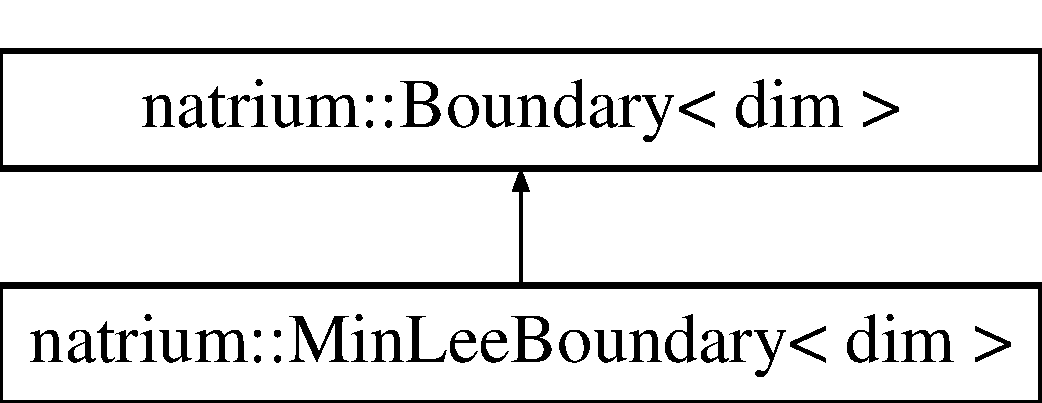
\includegraphics[height=2cm]{classnatrium_1_1MinLeeBoundary}
\end{center}
\end{figure}
\subsection*{Public Member Functions}
\begin{DoxyCompactItemize}
\item 
\hypertarget{classnatrium_1_1MinLeeBoundary_a1e9acd91ee2b97783932c4df45d38668}{
\hyperlink{classnatrium_1_1MinLeeBoundary_a1e9acd91ee2b97783932c4df45d38668}{MinLeeBoundary} (size\_\-t boundaryIndicator, shared\_\-ptr$<$ dealii::Function$<$ dim $>$ $>$ boundaryDensity, shared\_\-ptr$<$ dealii::Function$<$ dim $>$ $>$ boundaryVelocity)}
\label{classnatrium_1_1MinLeeBoundary_a1e9acd91ee2b97783932c4df45d38668}

\begin{DoxyCompactList}\small\item\em constructor \item\end{DoxyCompactList}\item 
\hypertarget{classnatrium_1_1MinLeeBoundary_a6bd31d48ffaf23ac74bc303b379b4ca8}{
\hyperlink{classnatrium_1_1MinLeeBoundary_a6bd31d48ffaf23ac74bc303b379b4ca8}{MinLeeBoundary} (size\_\-t boundaryIndicator, const dealii::Vector$<$ double $>$ \&velocity)}
\label{classnatrium_1_1MinLeeBoundary_a6bd31d48ffaf23ac74bc303b379b4ca8}

\begin{DoxyCompactList}\small\item\em constructor \item\end{DoxyCompactList}\item 
\hypertarget{classnatrium_1_1MinLeeBoundary_ab2409b8dceb378d7e2bdb457e8c5f374}{
virtual \hyperlink{classnatrium_1_1MinLeeBoundary_ab2409b8dceb378d7e2bdb457e8c5f374}{$\sim$MinLeeBoundary} ()}
\label{classnatrium_1_1MinLeeBoundary_ab2409b8dceb378d7e2bdb457e8c5f374}

\begin{DoxyCompactList}\small\item\em destructor \item\end{DoxyCompactList}\item 
void \hyperlink{classnatrium_1_1MinLeeBoundary_a9d9b16e12b09af906b21cae27102e1c3}{addToSparsityPattern} (dealii::DynamicSparsityPattern \&cSparse, const dealii::DoFHandler$<$ dim $>$ \&doFHandler, const \hyperlink{classnatrium_1_1Stencil}{Stencil} \&) const 
\begin{DoxyCompactList}\small\item\em modify sparsity pattern so that the fluxes over periodic boundary can be incorporated \item\end{DoxyCompactList}\item 
void \hyperlink{classnatrium_1_1MinLeeBoundary_ac23616963c4e9873c2177cdc7f67e159}{assembleBoundary} (size\_\-t alpha, const typename dealii::DoFHandler$<$ dim $>$::active\_\-cell\_\-iterator \&cell, size\_\-t faceNumber, dealii::FEFaceValues$<$ dim $>$ \&feFaceValues, const \hyperlink{classnatrium_1_1Stencil}{Stencil} \&stencil, const std::map$<$ size\_\-t, size\_\-t $>$ \&q\_\-index\_\-to\_\-facedof, const vector$<$ double $>$ \&inverseLocalMassMatrix, distributed\_\-sparse\_\-block\_\-matrix \&systemMatrix, distributed\_\-block\_\-vector \&systemVector, bool useCentralFlux=false) const 
\item 
\hypertarget{classnatrium_1_1MinLeeBoundary_a050f00caec37ee8e2f6e19a4d3d2d1fc}{
size\_\-t {\bfseries getBoundaryIndicator} () const }
\label{classnatrium_1_1MinLeeBoundary_a050f00caec37ee8e2f6e19a4d3d2d1fc}

\end{DoxyCompactItemize}


\subsection{Detailed Description}
\subsubsection*{template$<$size\_\-t dim$>$ class natrium::MinLeeBoundary$<$ dim $>$}

The boundary described by Min and Lee. For outgoing particle distribution functions the fluxes are set to 0 For incoming particle distributions fluxes are set to \[ f_{\alpha} - f^{+}_{\alpha} = f_{\alpha} - f_{\alpha^{*}} - 2w_{\alpha} \rho_{0} (e_{\alpha}\cdot u_{b})/c^{2}_{s}\]. 

\subsection{Member Function Documentation}
\hypertarget{classnatrium_1_1MinLeeBoundary_a9d9b16e12b09af906b21cae27102e1c3}{
\index{natrium::MinLeeBoundary@{natrium::MinLeeBoundary}!addToSparsityPattern@{addToSparsityPattern}}
\index{addToSparsityPattern@{addToSparsityPattern}!natrium::MinLeeBoundary@{natrium::MinLeeBoundary}}
\subsubsection[{addToSparsityPattern}]{\setlength{\rightskip}{0pt plus 5cm}template$<$size\_\-t dim$>$ void {\bf natrium::MinLeeBoundary}$<$ dim $>$::addToSparsityPattern (dealii::DynamicSparsityPattern \& {\em cSparse}, \/  const dealii::DoFHandler$<$ dim $>$ \& {\em doFHandler}, \/  const {\bf Stencil} \&) const\hspace{0.3cm}{\ttfamily  \mbox{[}inline\mbox{]}}}}
\label{classnatrium_1_1MinLeeBoundary_a9d9b16e12b09af906b21cae27102e1c3}


modify sparsity pattern so that the fluxes over periodic boundary can be incorporated 
\begin{DoxyParams}{Parameters}
\item[{\em cSparse}]the block-\/sparsity pattern \end{DoxyParams}
\hypertarget{classnatrium_1_1MinLeeBoundary_ac23616963c4e9873c2177cdc7f67e159}{
\index{natrium::MinLeeBoundary@{natrium::MinLeeBoundary}!assembleBoundary@{assembleBoundary}}
\index{assembleBoundary@{assembleBoundary}!natrium::MinLeeBoundary@{natrium::MinLeeBoundary}}
\subsubsection[{assembleBoundary}]{\setlength{\rightskip}{0pt plus 5cm}template$<$size\_\-t dim$>$ void {\bf natrium::MinLeeBoundary}$<$ dim $>$::assembleBoundary (size\_\-t {\em alpha}, \/  const typename dealii::DoFHandler$<$ dim $>$::active\_\-cell\_\-iterator \& {\em cell}, \/  size\_\-t {\em faceNumber}, \/  dealii::FEFaceValues$<$ dim $>$ \& {\em feFaceValues}, \/  const {\bf Stencil} \& {\em stencil}, \/  const std::map$<$ size\_\-t, size\_\-t $>$ \& {\em q\_\-index\_\-to\_\-facedof}, \/  const vector$<$ double $>$ \& {\em inverseLocalMassMatrix}, \/  distributed\_\-sparse\_\-block\_\-matrix \& {\em systemMatrix}, \/  distributed\_\-block\_\-vector \& {\em systemVector}, \/  bool {\em useCentralFlux} = {\ttfamily false}) const\hspace{0.3cm}{\ttfamily  \mbox{[}inline\mbox{]}}}}
\label{classnatrium_1_1MinLeeBoundary_ac23616963c4e9873c2177cdc7f67e159}


Distribute to global matrix 

The documentation for this class was generated from the following files:\begin{DoxyCompactItemize}
\item 
/mnt/fdrive/akraem3m/workspace/NATriuM/src/library/natrium/problemdescription/\hyperlink{MinLeeBoundary_8h}{MinLeeBoundary.h}\item 
/mnt/fdrive/akraem3m/workspace/NATriuM/src/library/natrium/problemdescription/MinLeeBoundary.cpp\end{DoxyCompactItemize}

\hypertarget{classnatrium_1_1MPIGuard}{
\section{natrium::MPIGuard Class Reference}
\label{classnatrium_1_1MPIGuard}\index{natrium::MPIGuard@{natrium::MPIGuard}}
}


Singleton that encapsulates the MPI init and finalize calls so that they are called at most once per run. This class wraps the function dealii::Utilities::MPI::MPI\_\-InitFinalize(argc, argv).  


{\ttfamily \#include $<$MPIGuard.h$>$}\subsection*{Public Member Functions}
\begin{DoxyCompactItemize}
\item 
\hypertarget{classnatrium_1_1MPIGuard_a1e07fafea3f7724d0d2dd9c106e1a44b}{
\hyperlink{classnatrium_1_1MPIGuard_a1e07fafea3f7724d0d2dd9c106e1a44b}{MPIGuard} (int \&argc, char $\ast$$\ast$\&argv)}
\label{classnatrium_1_1MPIGuard_a1e07fafea3f7724d0d2dd9c106e1a44b}

\begin{DoxyCompactList}\small\item\em Constructor (should normally be private, but is not allowed by boost::make\_\-shared). \item\end{DoxyCompactList}\item 
\hypertarget{classnatrium_1_1MPIGuard_a4df8a28efa88e97a77ee0dc9a74a1a17}{
boost::shared\_\-ptr$<$ dealii::Utilities::MPI::MPI\_\-InitFinalize $>$ \hyperlink{classnatrium_1_1MPIGuard_a4df8a28efa88e97a77ee0dc9a74a1a17}{getMPI\_\-InitFinalize} ()}
\label{classnatrium_1_1MPIGuard_a4df8a28efa88e97a77ee0dc9a74a1a17}

\begin{DoxyCompactList}\small\item\em return dealii's MPI\_\-InitFinalize object \item\end{DoxyCompactList}\end{DoxyCompactItemize}
\subsection*{Static Public Member Functions}
\begin{DoxyCompactItemize}
\item 
\hypertarget{classnatrium_1_1MPIGuard_a1ff461f2c920911f2ac67b4ddc57ecdc}{
static boost::shared\_\-ptr$<$ \hyperlink{classnatrium_1_1MPIGuard}{MPIGuard} $>$ \hyperlink{classnatrium_1_1MPIGuard_a1ff461f2c920911f2ac67b4ddc57ecdc}{getInstance} (int \&argc, char $\ast$$\ast$\&argv)}
\label{classnatrium_1_1MPIGuard_a1ff461f2c920911f2ac67b4ddc57ecdc}

\begin{DoxyCompactList}\small\item\em Static constructor.  Command line argument. Can be used to determine the number of parallel processes. See documentation of dealii::Utilities::MPI::MPI\_\-InitFinalize(argc, argv) for details.  Command line argument.Can be used to determine the number of parallel processes. See documentation of dealii::Utilities::MPI::MPI\_\-InitFinalize(argc, argv) for details. \item\end{DoxyCompactList}\item 
\hypertarget{classnatrium_1_1MPIGuard_a5896abef9f379f89b746e71c4d3e68aa}{
static boost::shared\_\-ptr$<$ \hyperlink{classnatrium_1_1MPIGuard}{MPIGuard} $>$ {\bfseries getInstance} ()}
\label{classnatrium_1_1MPIGuard_a5896abef9f379f89b746e71c4d3e68aa}

\end{DoxyCompactItemize}


\subsection{Detailed Description}
Singleton that encapsulates the MPI init and finalize calls so that they are called at most once per run. This class wraps the function dealii::Utilities::MPI::MPI\_\-InitFinalize(argc, argv). 

The documentation for this class was generated from the following files:\begin{DoxyCompactItemize}
\item 
/mnt/fdrive/akraem3m/workspace/NATriuM/src/library/natrium/utilities/MPIGuard.h\item 
/mnt/fdrive/akraem3m/workspace/NATriuM/src/library/natrium/utilities/MPIGuard.cpp\end{DoxyCompactItemize}

\hypertarget{classnatrium_1_1own__double__less}{\section{natrium\-:\-:own\-\_\-double\-\_\-less Class Reference}
\label{classnatrium_1_1own__double__less}\index{natrium\-::own\-\_\-double\-\_\-less@{natrium\-::own\-\_\-double\-\_\-less}}
}


function to compare doubles as map keys; regards two doubles equal if they are in a epsilon(=1e-\/7)-\/range.  




{\ttfamily \#include $<$Math.\-h$>$}

Inheritance diagram for natrium\-:\-:own\-\_\-double\-\_\-less\-:\begin{figure}[H]
\begin{center}
\leavevmode
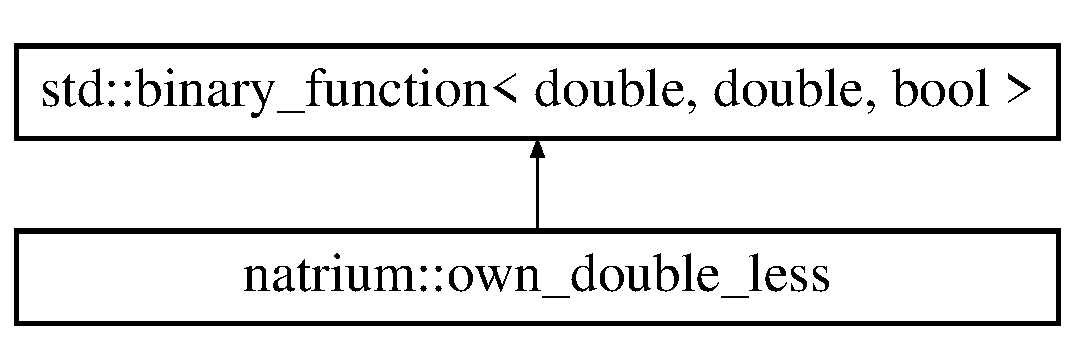
\includegraphics[height=2.000000cm]{classnatrium_1_1own__double__less}
\end{center}
\end{figure}
\subsection*{Public Member Functions}
\begin{DoxyCompactItemize}
\item 
\hypertarget{classnatrium_1_1own__double__less_ad0801e961db1be7a8752237d551bb016}{{\bfseries own\-\_\-double\-\_\-less} (double arg\-\_\-=1e-\/8)}\label{classnatrium_1_1own__double__less_ad0801e961db1be7a8752237d551bb016}

\item 
\hypertarget{classnatrium_1_1own__double__less_a79f21afda2b0b72708c20ce78080dbc7}{bool {\bfseries operator()} (const double \&left, const double \&right) const }\label{classnatrium_1_1own__double__less_a79f21afda2b0b72708c20ce78080dbc7}

\end{DoxyCompactItemize}
\subsection*{Public Attributes}
\begin{DoxyCompactItemize}
\item 
\hypertarget{classnatrium_1_1own__double__less_a5de868df983787412438c481c21621a7}{double {\bfseries epsilon}}\label{classnatrium_1_1own__double__less_a5de868df983787412438c481c21621a7}

\end{DoxyCompactItemize}


\subsection{Detailed Description}
function to compare doubles as map keys; regards two doubles equal if they are in a epsilon(=1e-\/7)-\/range. 

The documentation for this class was generated from the following file\-:\begin{DoxyCompactItemize}
\item 
/home/kraemer/eclipse\-\_\-workspace/\-N\-A\-Triu\-M/src/natrium/utilities/\hyperlink{Math_8h}{Math.\-h}\end{DoxyCompactItemize}

\hypertarget{classnatrium_1_1PeriodicBoundary}{
\section{natrium::PeriodicBoundary$<$ dim $>$ Class Template Reference}
\label{classnatrium_1_1PeriodicBoundary}\index{natrium::PeriodicBoundary@{natrium::PeriodicBoundary}}
}


A periodic boundary condition. Periodic boundaries have to be set before the grid is refined!  


{\ttfamily \#include $<$PeriodicBoundary.h$>$}Inheritance diagram for natrium::PeriodicBoundary$<$ dim $>$::\begin{figure}[H]
\begin{center}
\leavevmode
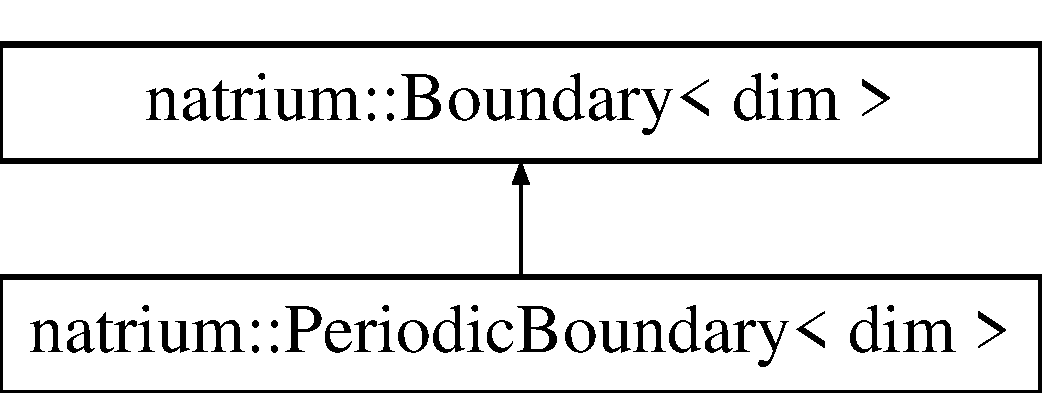
\includegraphics[height=2cm]{classnatrium_1_1PeriodicBoundary}
\end{center}
\end{figure}
\subsection*{Public Member Functions}
\begin{DoxyCompactItemize}
\item 
\hyperlink{classnatrium_1_1PeriodicBoundary_ad105994a331755f654822813875771d8}{PeriodicBoundary} (size\_\-t boundaryIndicator1, size\_\-t boundaryIndicator2, size\_\-t direction, boost::shared\_\-ptr$<$ Mesh$<$ dim $>$ $>$ triangulation)
\begin{DoxyCompactList}\small\item\em Constructor; the periodic boundary is defined by two lines. The degrees of freedom on the first line are forced to be equal to the opposite one on the second line, respectively. \item\end{DoxyCompactList}\item 
\hypertarget{classnatrium_1_1PeriodicBoundary_ad5f86b54a5a3ff86593ddb0e69b352e4}{
virtual \hyperlink{classnatrium_1_1PeriodicBoundary_ad5f86b54a5a3ff86593ddb0e69b352e4}{$\sim$PeriodicBoundary} ()}
\label{classnatrium_1_1PeriodicBoundary_ad5f86b54a5a3ff86593ddb0e69b352e4}

\begin{DoxyCompactList}\small\item\em destructor \item\end{DoxyCompactList}\item 
size\_\-t \hyperlink{classnatrium_1_1PeriodicBoundary_aaa861135e070feb4b3dd4408c487cd14}{getOppositeCellAtPeriodicBoundary} (const typename dealii::DoFHandler$<$ dim $>$::active\_\-cell\_\-iterator \&cell, typename dealii::DoFHandler$<$ dim $>$::cell\_\-iterator \&neighborCell) const 
\begin{DoxyCompactList}\small\item\em get the respective neighbor cell on the other side of a periodic boundary \item\end{DoxyCompactList}\item 
bool \hyperlink{classnatrium_1_1PeriodicBoundary_af43c1306653cc8a9d5aea68edcfca370}{isFaceInBoundary} (const typename dealii::DoFHandler$<$ dim $>$::active\_\-cell\_\-iterator \&, size\_\-t faceBoundaryIndicator) const 
\begin{DoxyCompactList}\small\item\em test if a given face belongs to this boundary \item\end{DoxyCompactList}\item 
\hypertarget{classnatrium_1_1PeriodicBoundary_a38c5e966e4b2a1ee185a5634fc379393}{
virtual bool \hyperlink{classnatrium_1_1PeriodicBoundary_a38c5e966e4b2a1ee185a5634fc379393}{isPeriodic} () const }
\label{classnatrium_1_1PeriodicBoundary_a38c5e966e4b2a1ee185a5634fc379393}

\begin{DoxyCompactList}\small\item\em is the boundary a periodic boundary ? \item\end{DoxyCompactList}\item 
void \hyperlink{classnatrium_1_1PeriodicBoundary_a233d460baa307b13bc32efb57c07f7c5}{createCellMap} (const dealii::DoFHandler$<$ dim $>$ \&doFHandler)
\begin{DoxyCompactList}\small\item\em create the map m\_\-cells which stores the cells adjacent to the periodic boundary \item\end{DoxyCompactList}\item 
\hypertarget{classnatrium_1_1PeriodicBoundary_a4885d5d5d4c8965db5534390ad877511}{
void \hyperlink{classnatrium_1_1PeriodicBoundary_a4885d5d5d4c8965db5534390ad877511}{checkCellMap} ()}
\label{classnatrium_1_1PeriodicBoundary_a4885d5d5d4c8965db5534390ad877511}

\begin{DoxyCompactList}\small\item\em check if all cells in the cell map have appropriate boundary indicators \item\end{DoxyCompactList}\item 
\hypertarget{classnatrium_1_1PeriodicBoundary_af46e4e91a6b612fb3b2ef658b962d5d8}{
void \hyperlink{classnatrium_1_1PeriodicBoundary_af46e4e91a6b612fb3b2ef658b962d5d8}{addToSparsityPattern} (dealii::BlockDynamicSparsityPattern \&, size\_\-t, size\_\-t, size\_\-t) const }
\label{classnatrium_1_1PeriodicBoundary_af46e4e91a6b612fb3b2ef658b962d5d8}

\begin{DoxyCompactList}\small\item\em This function does nothing; just to satisfy the interface. The Periodic \hyperlink{classnatrium_1_1Boundary}{Boundary} conditions are directly incorporated in make\_\-sparser\_\-flux\_\-sparsity\_\-pattern. \item\end{DoxyCompactList}\item 
dealii::Point$<$ dim $>$ \hyperlink{classnatrium_1_1PeriodicBoundary_a9a5677bbc1d59499ceec15a7893b8688}{coordinatesAcrossPeriodicBoundary} (const dealii::Point$<$ dim $>$ \&p, const typename dealii::DoFHandler$<$ dim $>$::active\_\-cell\_\-iterator \&cell)
\item 
\hypertarget{classnatrium_1_1PeriodicBoundary_a1351b925b9ae2008539a351a4baac3e0}{
const boost::shared\_\-ptr$<$ Mesh$<$ dim $>$ $>$ \& {\bfseries getMesh} () const }
\label{classnatrium_1_1PeriodicBoundary_a1351b925b9ae2008539a351a4baac3e0}

\item 
\hypertarget{classnatrium_1_1PeriodicBoundary_aead325214d43693a03a5d24613f4fe14}{
size\_\-t {\bfseries getBoundaryIndicator1} () const }
\label{classnatrium_1_1PeriodicBoundary_aead325214d43693a03a5d24613f4fe14}

\item 
\hypertarget{classnatrium_1_1PeriodicBoundary_af7e6f5b6028b0499df8335377156bc26}{
size\_\-t {\bfseries getBoundaryIndicator2} () const }
\label{classnatrium_1_1PeriodicBoundary_af7e6f5b6028b0499df8335377156bc26}

\item 
\hypertarget{classnatrium_1_1PeriodicBoundary_a4200caafcbda9553552220303e26bad0}{
const PeriodicCellMap$<$ dim $>$ \& {\bfseries getCellMap} () const }
\label{classnatrium_1_1PeriodicBoundary_a4200caafcbda9553552220303e26bad0}

\item 
\hypertarget{classnatrium_1_1PeriodicBoundary_a49e51f3612f67060f6189c3f92f64025}{
size\_\-t {\bfseries getDirection} () const }
\label{classnatrium_1_1PeriodicBoundary_a49e51f3612f67060f6189c3f92f64025}

\item 
\hypertarget{classnatrium_1_1PeriodicBoundary_ac02d8bae511dcb9d63d5da8478f2cb03}{
const boost::shared\_\-ptr$<$ Mesh$<$ dim $>$ $>$ \& {\bfseries getTriangulation} () const }
\label{classnatrium_1_1PeriodicBoundary_ac02d8bae511dcb9d63d5da8478f2cb03}

\end{DoxyCompactItemize}
\subsection*{Friends}
\begin{DoxyCompactItemize}
\item 
\hypertarget{classnatrium_1_1PeriodicBoundary_a92462e8f67aa8d5e91e018a1cce70842}{
class {\bfseries own\_\-double\_\-less\_\-periodic}}
\label{classnatrium_1_1PeriodicBoundary_a92462e8f67aa8d5e91e018a1cce70842}

\end{DoxyCompactItemize}


\subsection{Detailed Description}
\subsubsection*{template$<$size\_\-t dim$>$ class natrium::PeriodicBoundary$<$ dim $>$}

A periodic boundary condition. Periodic boundaries have to be set before the grid is refined! \begin{DoxyNote}{Note}
First use in step-\/1 tutorial. 
\end{DoxyNote}


\subsection{Constructor \& Destructor Documentation}
\hypertarget{classnatrium_1_1PeriodicBoundary_ad105994a331755f654822813875771d8}{
\index{natrium::PeriodicBoundary@{natrium::PeriodicBoundary}!PeriodicBoundary@{PeriodicBoundary}}
\index{PeriodicBoundary@{PeriodicBoundary}!natrium::PeriodicBoundary@{natrium::PeriodicBoundary}}
\subsubsection[{PeriodicBoundary}]{\setlength{\rightskip}{0pt plus 5cm}template$<$size\_\-t dim$>$ {\bf natrium::PeriodicBoundary}$<$ dim $>$::{\bf PeriodicBoundary} (size\_\-t {\em boundaryIndicator1}, \/  size\_\-t {\em boundaryIndicator2}, \/  size\_\-t {\em direction}, \/  boost::shared\_\-ptr$<$ Mesh$<$ dim $>$ $>$ {\em triangulation})\hspace{0.3cm}{\ttfamily  \mbox{[}inline\mbox{]}}}}
\label{classnatrium_1_1PeriodicBoundary_ad105994a331755f654822813875771d8}


Constructor; the periodic boundary is defined by two lines. The degrees of freedom on the first line are forced to be equal to the opposite one on the second line, respectively. DEPRECATED, because boundary indicators are needed for application of boundary values \begin{DoxyNote}{Note}
Since both lines have to match each other perfectly, the constructor tests whether their lengths agree.
\end{DoxyNote}

\begin{DoxyParams}{Parameters}
\item[{\em beginLine1}]start point of line 1 \item[{\em endLine1}]end point of line 1 \item[{\em beginLine2}]start point of line 2 \item[{\em endLine2}]end point of line 2 PeriodicBoundary1D(dealii::Point$<$2$>$\& beginLine1, dealii::Point$<$2$>$\& endLine1, dealii::Point$<$2$>$\& beginLine2, dealii::Point$<$2$>$\& endLine2, boost::shared\_\-ptr$<$Mesh$<$2$>$ $>$ triangulation); Constructor; the periodic boundary is defined by two lines. The degrees of freedom on the first line are forced to be equal to the opposite one on the second line, respectively. \end{DoxyParams}
\begin{DoxyNote}{Note}
Since both lines have to match each other perfectly, the constructor tests whether their lengths agree.
\end{DoxyNote}

\begin{DoxyParams}{Parameters}
\item[{\em boundaryIndicator1}]boundary indicator of interface line 1 \item[{\em boundaryIndicator2}]boundary indicator of interface line 2 \item[{\em triangulation}]A (shared ptr to a) triangulation object (the mesh) \end{DoxyParams}


\subsection{Member Function Documentation}
\hypertarget{classnatrium_1_1PeriodicBoundary_a9a5677bbc1d59499ceec15a7893b8688}{
\index{natrium::PeriodicBoundary@{natrium::PeriodicBoundary}!coordinatesAcrossPeriodicBoundary@{coordinatesAcrossPeriodicBoundary}}
\index{coordinatesAcrossPeriodicBoundary@{coordinatesAcrossPeriodicBoundary}!natrium::PeriodicBoundary@{natrium::PeriodicBoundary}}
\subsubsection[{coordinatesAcrossPeriodicBoundary}]{\setlength{\rightskip}{0pt plus 5cm}template$<$size\_\-t dim$>$ dealii::Point$<$ dim $>$ {\bf natrium::PeriodicBoundary}$<$ dim $>$::coordinatesAcrossPeriodicBoundary (const dealii::Point$<$ dim $>$ \& {\em p}, \/  const typename dealii::DoFHandler$<$ dim $>$::active\_\-cell\_\-iterator \& {\em cell})\hspace{0.3cm}{\ttfamily  \mbox{[}inline\mbox{]}}}}
\label{classnatrium_1_1PeriodicBoundary_a9a5677bbc1d59499ceec15a7893b8688}
Transform a point into its equivalent across the periodic boundary \hypertarget{classnatrium_1_1PeriodicBoundary_a233d460baa307b13bc32efb57c07f7c5}{
\index{natrium::PeriodicBoundary@{natrium::PeriodicBoundary}!createCellMap@{createCellMap}}
\index{createCellMap@{createCellMap}!natrium::PeriodicBoundary@{natrium::PeriodicBoundary}}
\subsubsection[{createCellMap}]{\setlength{\rightskip}{0pt plus 5cm}template$<$size\_\-t dim$>$ void {\bf natrium::PeriodicBoundary}$<$ dim $>$::createCellMap (const dealii::DoFHandler$<$ dim $>$ \& {\em doFHandler})\hspace{0.3cm}{\ttfamily  \mbox{[}inline\mbox{]}}}}
\label{classnatrium_1_1PeriodicBoundary_a233d460baa307b13bc32efb57c07f7c5}


create the map m\_\-cells which stores the cells adjacent to the periodic boundary 
\begin{DoxyParams}{Parameters}
\item[{\em doFHandler}]The map is stored with doFHandler iterators in order to access degrees of freedom at the boundary. \end{DoxyParams}
\hypertarget{classnatrium_1_1PeriodicBoundary_aaa861135e070feb4b3dd4408c487cd14}{
\index{natrium::PeriodicBoundary@{natrium::PeriodicBoundary}!getOppositeCellAtPeriodicBoundary@{getOppositeCellAtPeriodicBoundary}}
\index{getOppositeCellAtPeriodicBoundary@{getOppositeCellAtPeriodicBoundary}!natrium::PeriodicBoundary@{natrium::PeriodicBoundary}}
\subsubsection[{getOppositeCellAtPeriodicBoundary}]{\setlength{\rightskip}{0pt plus 5cm}template$<$size\_\-t dim$>$ size\_\-t {\bf natrium::PeriodicBoundary}$<$ dim $>$::getOppositeCellAtPeriodicBoundary (const typename dealii::DoFHandler$<$ dim $>$::active\_\-cell\_\-iterator \& {\em cell}, \/  typename dealii::DoFHandler$<$ dim $>$::cell\_\-iterator \& {\em neighborCell}) const\hspace{0.3cm}{\ttfamily  \mbox{[}inline\mbox{]}}}}
\label{classnatrium_1_1PeriodicBoundary_aaa861135e070feb4b3dd4408c487cd14}


get the respective neighbor cell on the other side of a periodic boundary 
\begin{DoxyParams}{Parameters}
\item[\mbox{$\leftarrow$} {\em cellID}]a cell ID \item[\mbox{$\rightarrow$} {\em neighborCell}]the desired neighbor cell\end{DoxyParams}
\begin{DoxyReturn}{Returns}
local face number of cell1, denoting the respective cell number 
\end{DoxyReturn}
\hypertarget{classnatrium_1_1PeriodicBoundary_af43c1306653cc8a9d5aea68edcfca370}{
\index{natrium::PeriodicBoundary@{natrium::PeriodicBoundary}!isFaceInBoundary@{isFaceInBoundary}}
\index{isFaceInBoundary@{isFaceInBoundary}!natrium::PeriodicBoundary@{natrium::PeriodicBoundary}}
\subsubsection[{isFaceInBoundary}]{\setlength{\rightskip}{0pt plus 5cm}template$<$size\_\-t dim$>$ bool {\bf natrium::PeriodicBoundary}$<$ dim $>$::isFaceInBoundary (const typename dealii::DoFHandler$<$ dim $>$::active\_\-cell\_\-iterator \&, \/  size\_\-t {\em faceBoundaryIndicator}) const\hspace{0.3cm}{\ttfamily  \mbox{[}inline\mbox{]}}}}
\label{classnatrium_1_1PeriodicBoundary_af43c1306653cc8a9d5aea68edcfca370}


test if a given face belongs to this boundary 
\begin{DoxyParams}{Parameters}
\item[\mbox{$\leftarrow$} {\em cell}]pointer to the cell \item[\mbox{$\leftarrow$} {\em faceBoundaryIndicator}]the boundary indicator of the face \end{DoxyParams}


The documentation for this class was generated from the following files:\begin{DoxyCompactItemize}
\item 
/mnt/fdrive/akraem3m/workspace/NATriuM/src/library/natrium/boundaries/\hyperlink{PeriodicBoundary_8h}{PeriodicBoundary.h}\item 
/mnt/fdrive/akraem3m/workspace/NATriuM/src/library/natrium/boundaries/\hyperlink{PeriodicBoundary_8cpp}{PeriodicBoundary.cpp}\end{DoxyCompactItemize}

\hypertarget{classnatrium_1_1PeriodicBoundaryNotPossible}{
\section{natrium::PeriodicBoundaryNotPossible Class Reference}
\label{classnatrium_1_1PeriodicBoundaryNotPossible}\index{natrium::PeriodicBoundaryNotPossible@{natrium::PeriodicBoundaryNotPossible}}
}


Exception for impossible periodic boundary, e.g. when the interfaces don't have the same length.  


{\ttfamily \#include $<$PeriodicBoundary.h$>$}Inheritance diagram for natrium::PeriodicBoundaryNotPossible::\begin{figure}[H]
\begin{center}
\leavevmode
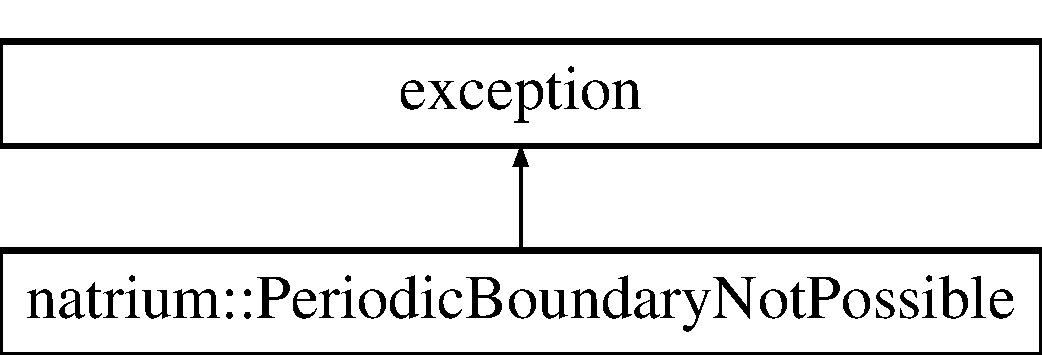
\includegraphics[height=2cm]{classnatrium_1_1PeriodicBoundaryNotPossible}
\end{center}
\end{figure}
\subsection*{Public Member Functions}
\begin{DoxyCompactItemize}
\item 
\hypertarget{classnatrium_1_1PeriodicBoundaryNotPossible_ad5eb4588e496d08cea9b623df1372807}{
{\bfseries PeriodicBoundaryNotPossible} (const char $\ast$msg, const std::stringstream \&additionalInfo=std::stringstream())}
\label{classnatrium_1_1PeriodicBoundaryNotPossible_ad5eb4588e496d08cea9b623df1372807}

\item 
\hypertarget{classnatrium_1_1PeriodicBoundaryNotPossible_a4597b7a3a3e34233911fe8e1dd7bc5f4}{
{\bfseries PeriodicBoundaryNotPossible} (const string \&msg, const std::stringstream \&additionalInfo=std::stringstream())}
\label{classnatrium_1_1PeriodicBoundaryNotPossible_a4597b7a3a3e34233911fe8e1dd7bc5f4}

\item 
\hypertarget{classnatrium_1_1PeriodicBoundaryNotPossible_a32746bddb45dc92e28e8aef98ceed310}{
const char $\ast$ {\bfseries what} () const   throw ()}
\label{classnatrium_1_1PeriodicBoundaryNotPossible_a32746bddb45dc92e28e8aef98ceed310}

\end{DoxyCompactItemize}


\subsection{Detailed Description}
Exception for impossible periodic boundary, e.g. when the interfaces don't have the same length. 

The documentation for this class was generated from the following file:\begin{DoxyCompactItemize}
\item 
/mnt/fdrive/akraem3m/workspace/NATriuM/src/library/natrium/problemdescription/\hyperlink{PeriodicBoundary_8h}{PeriodicBoundary.h}\end{DoxyCompactItemize}

\hypertarget{classnatrium_1_1PeriodicTestDomain2D}{
\section{natrium::PeriodicTestDomain2D Class Reference}
\label{classnatrium_1_1PeriodicTestDomain2D}\index{natrium::PeriodicTestDomain2D@{natrium::PeriodicTestDomain2D}}
}


Description of a simple Periodic Flow (flow in square domain). The domain is \mbox{[}0,1\mbox{]}$^\wedge$2. The domain consists of 4 elements.  


{\ttfamily \#include $<$PeriodicTestDomain2D.h$>$}Inheritance diagram for natrium::PeriodicTestDomain2D::\begin{figure}[H]
\begin{center}
\leavevmode
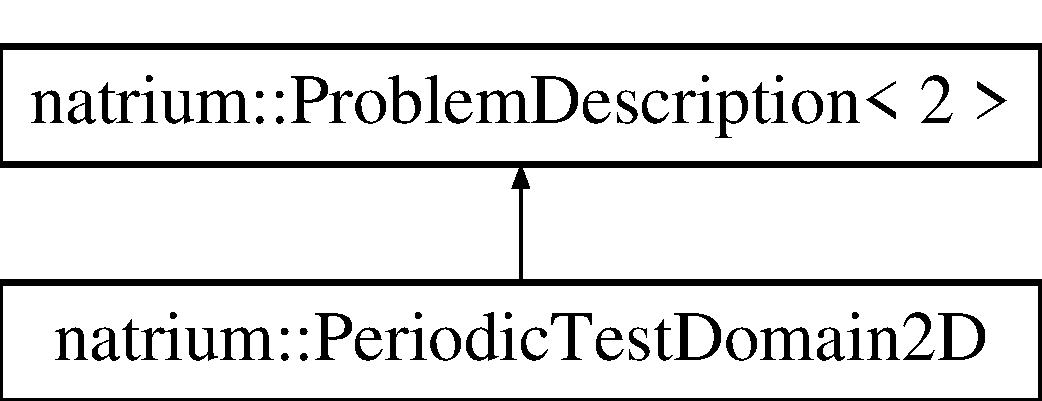
\includegraphics[height=2cm]{classnatrium_1_1PeriodicTestDomain2D}
\end{center}
\end{figure}
\subsection*{Public Member Functions}
\begin{DoxyCompactItemize}
\item 
\hyperlink{classnatrium_1_1PeriodicTestDomain2D_a930da37a3e1be744aaf59e27ba956318}{PeriodicTestDomain2D} (size\_\-t globalRefinementLevel)
\begin{DoxyCompactList}\small\item\em constructor \item\end{DoxyCompactList}\item 
\hypertarget{classnatrium_1_1PeriodicTestDomain2D_a81fe3504b294cd4d6219c360f465f84b}{
virtual \hyperlink{classnatrium_1_1PeriodicTestDomain2D_a81fe3504b294cd4d6219c360f465f84b}{$\sim$PeriodicTestDomain2D} ()}
\label{classnatrium_1_1PeriodicTestDomain2D_a81fe3504b294cd4d6219c360f465f84b}

\begin{DoxyCompactList}\small\item\em destructor \item\end{DoxyCompactList}\item 
\hypertarget{classnatrium_1_1PeriodicTestDomain2D_a2585d064816ca884d12586da93388a48}{
virtual void {\bfseries refine} (Mesh$<$ 2 $>$ \&mesh)}
\label{classnatrium_1_1PeriodicTestDomain2D_a2585d064816ca884d12586da93388a48}

\item 
\hypertarget{classnatrium_1_1PeriodicTestDomain2D_a1a6e52d1a6b3f09332158ecbf19eab6e}{
virtual void {\bfseries transform} (Mesh$<$ 2 $>$ \&)}
\label{classnatrium_1_1PeriodicTestDomain2D_a1a6e52d1a6b3f09332158ecbf19eab6e}

\end{DoxyCompactItemize}


\subsection{Detailed Description}
Description of a simple Periodic Flow (flow in square domain). The domain is \mbox{[}0,1\mbox{]}$^\wedge$2. The domain consists of 4 elements. 

\subsection{Constructor \& Destructor Documentation}
\hypertarget{classnatrium_1_1PeriodicTestDomain2D_a930da37a3e1be744aaf59e27ba956318}{
\index{natrium::PeriodicTestDomain2D@{natrium::PeriodicTestDomain2D}!PeriodicTestDomain2D@{PeriodicTestDomain2D}}
\index{PeriodicTestDomain2D@{PeriodicTestDomain2D}!natrium::PeriodicTestDomain2D@{natrium::PeriodicTestDomain2D}}
\subsubsection[{PeriodicTestDomain2D}]{\setlength{\rightskip}{0pt plus 5cm}natrium::PeriodicTestDomain2D::PeriodicTestDomain2D (size\_\-t {\em globalRefinementLevel})}}
\label{classnatrium_1_1PeriodicTestDomain2D_a930da37a3e1be744aaf59e27ba956318}


constructor 

apply boundary values 

The documentation for this class was generated from the following files:\begin{DoxyCompactItemize}
\item 
/mnt/fdrive/akraem3m/workspace/NATriuM/src/library/natrium/benchmarks/\hyperlink{PeriodicTestDomain2D_8h}{PeriodicTestDomain2D.h}\item 
/mnt/fdrive/akraem3m/workspace/NATriuM/src/library/natrium/benchmarks/\hyperlink{PeriodicTestDomain2D_8cpp}{PeriodicTestDomain2D.cpp}\end{DoxyCompactItemize}

\hypertarget{classnatrium_1_1PhysicalProperties}{
\section{natrium::PhysicalProperties$<$ dim $>$ Class Template Reference}
\label{classnatrium_1_1PhysicalProperties}\index{natrium::PhysicalProperties@{natrium::PhysicalProperties}}
}
\subsection*{Public Member Functions}
\begin{DoxyCompactItemize}
\item 
\hypertarget{classnatrium_1_1PhysicalProperties_a5047491de09441e2aae00f6ba838f99e}{
\hyperlink{classnatrium_1_1PhysicalProperties_a5047491de09441e2aae00f6ba838f99e}{PhysicalProperties} ()}
\label{classnatrium_1_1PhysicalProperties_a5047491de09441e2aae00f6ba838f99e}

\begin{DoxyCompactList}\small\item\em constructor \item\end{DoxyCompactList}\item 
\hypertarget{classnatrium_1_1PhysicalProperties_a1089bbb66f56e8c31cdb2908d5b08757}{
virtual \hyperlink{classnatrium_1_1PhysicalProperties_a1089bbb66f56e8c31cdb2908d5b08757}{$\sim$PhysicalProperties} ()}
\label{classnatrium_1_1PhysicalProperties_a1089bbb66f56e8c31cdb2908d5b08757}

\begin{DoxyCompactList}\small\item\em destructor \item\end{DoxyCompactList}\item 
\hypertarget{classnatrium_1_1PhysicalProperties_a1a76b0dd1a88cfc037b85771c3166af7}{
{\footnotesize template$<$$>$ }\\double {\bfseries kineticEnergy} (const vector$<$ distributed\_\-vector $>$ \&u, const distributed\_\-vector \&rho, shared\_\-ptr$<$ \hyperlink{classnatrium_1_1AdvectionOperator}{AdvectionOperator}$<$ 2 $>$ $>$ advection)}
\label{classnatrium_1_1PhysicalProperties_a1a76b0dd1a88cfc037b85771c3166af7}

\item 
\hypertarget{classnatrium_1_1PhysicalProperties_abeda6e133c618f7eec4ccbeb08ef452e}{
{\footnotesize template$<$$>$ }\\double {\bfseries kineticEnergy} (const vector$<$ distributed\_\-vector $>$ \&u, const distributed\_\-vector \&rho, shared\_\-ptr$<$ \hyperlink{classnatrium_1_1AdvectionOperator}{AdvectionOperator}$<$ 3 $>$ $>$ advection)}
\label{classnatrium_1_1PhysicalProperties_abeda6e133c618f7eec4ccbeb08ef452e}

\end{DoxyCompactItemize}
\subsection*{Static Public Member Functions}
\begin{DoxyCompactItemize}
\item 
\hypertarget{classnatrium_1_1PhysicalProperties_ab813391c2437bca3edd626aac09a449f}{
static double {\bfseries kineticEnergy} (const vector$<$ distributed\_\-vector $>$ \&u, const distributed\_\-vector \&rho, shared\_\-ptr$<$ \hyperlink{classnatrium_1_1AdvectionOperator}{AdvectionOperator}$<$ dim $>$ $>$ advection)}
\label{classnatrium_1_1PhysicalProperties_ab813391c2437bca3edd626aac09a449f}

\item 
\hypertarget{classnatrium_1_1PhysicalProperties_a9041e6fc4bebe07da63c6f0b25aabc0d}{
static double \hyperlink{classnatrium_1_1PhysicalProperties_a9041e6fc4bebe07da63c6f0b25aabc0d}{maximalPressure} (const distributed\_\-vector \&rho, const double speedOfSound, double \&minimalPressure)}
\label{classnatrium_1_1PhysicalProperties_a9041e6fc4bebe07da63c6f0b25aabc0d}

\begin{DoxyCompactList}\small\item\em Pressure. \item\end{DoxyCompactList}\item 
\hypertarget{classnatrium_1_1PhysicalProperties_a34720f497e9659794dfe8e0ca2554f3a}{
static double \hyperlink{classnatrium_1_1PhysicalProperties_a34720f497e9659794dfe8e0ca2554f3a}{meanVelocityX} (const distributed\_\-vector \&ux, shared\_\-ptr$<$ \hyperlink{classnatrium_1_1AdvectionOperator}{AdvectionOperator}$<$ dim $>$ $>$ advection)}
\label{classnatrium_1_1PhysicalProperties_a34720f497e9659794dfe8e0ca2554f3a}

\begin{DoxyCompactList}\small\item\em Flow factor. \item\end{DoxyCompactList}\end{DoxyCompactItemize}
\subsubsection*{template$<$size\_\-t dim$>$ class natrium::PhysicalProperties$<$ dim $>$}



The documentation for this class was generated from the following files:\begin{DoxyCompactItemize}
\item 
/mnt/fdrive/akraem3m/workspace/NATriuM/src/library/natrium/solver/PhysicalProperties.h\item 
/mnt/fdrive/akraem3m/workspace/NATriuM/src/library/natrium/solver/\hyperlink{PhysicalProperties_8cpp}{PhysicalProperties.cpp}\end{DoxyCompactItemize}

\hypertarget{classnatrium_1_1PoiseuilleFlow2D}{\section{natrium\-:\-:Poiseuille\-Flow2\-D Class Reference}
\label{classnatrium_1_1PoiseuilleFlow2D}\index{natrium\-::\-Poiseuille\-Flow2\-D@{natrium\-::\-Poiseuille\-Flow2\-D}}
}


Description of a simple Channel Flow The domain is \mbox{[}0,5\mbox{]}x\mbox{[}0,1\mbox{]}.  




{\ttfamily \#include $<$Poiseuille\-Flow2\-D.\-h$>$}

Inheritance diagram for natrium\-:\-:Poiseuille\-Flow2\-D\-:\begin{figure}[H]
\begin{center}
\leavevmode
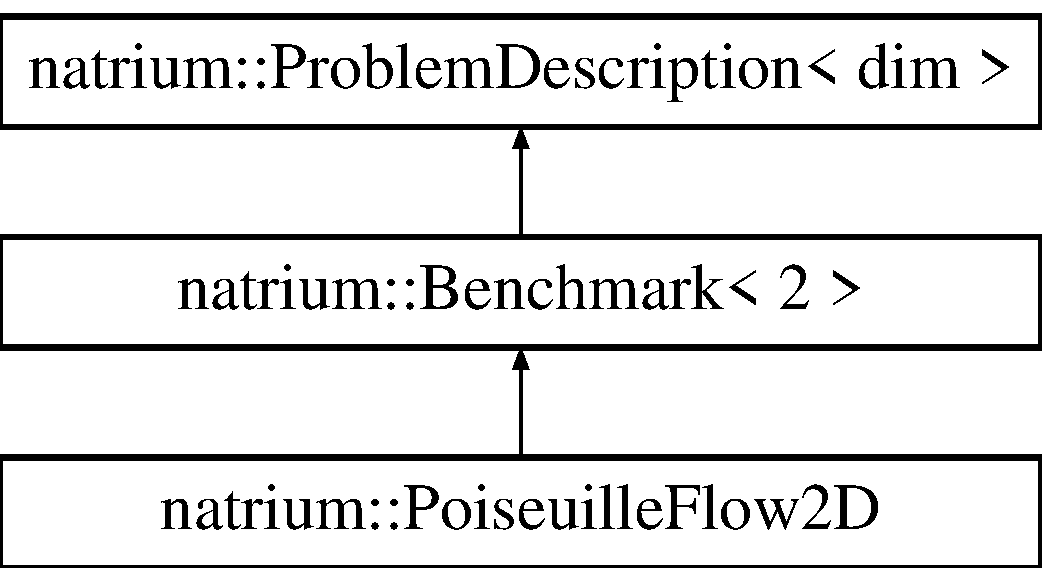
\includegraphics[height=2.000000cm]{classnatrium_1_1PoiseuilleFlow2D}
\end{center}
\end{figure}
\subsection*{Public Member Functions}
\begin{DoxyCompactItemize}
\item 
\hyperlink{classnatrium_1_1PoiseuilleFlow2D_a1834e3440ac19a8734f9133cd577e0ca}{Poiseuille\-Flow2\-D} (double viscosity, size\-\_\-t refinement\-Level)
\begin{DoxyCompactList}\small\item\em constructor \end{DoxyCompactList}\item 
\hypertarget{classnatrium_1_1PoiseuilleFlow2D_a62f9e7cfb2e32753b58eafb9d5936fd4}{virtual \hyperlink{classnatrium_1_1PoiseuilleFlow2D_a62f9e7cfb2e32753b58eafb9d5936fd4}{$\sim$\-Poiseuille\-Flow2\-D} ()}\label{classnatrium_1_1PoiseuilleFlow2D_a62f9e7cfb2e32753b58eafb9d5936fd4}

\begin{DoxyCompactList}\small\item\em destructor \end{DoxyCompactList}\item 
virtual void \hyperlink{classnatrium_1_1PoiseuilleFlow2D_a5f3475deac6f2666f181a052baf76502}{apply\-Initial\-Densities} (distributed\-\_\-vector \&initial\-Densities, vector$<$ dealii\-::\-Point$<$ 2 $>$ $>$ \&support\-Points) const 
\begin{DoxyCompactList}\small\item\em set initial densities \end{DoxyCompactList}\item 
virtual void \hyperlink{classnatrium_1_1PoiseuilleFlow2D_a8fe39ca61c90d194255e61d36c0681af}{apply\-Initial\-Velocities} (vector$<$ distributed\-\_\-vector $>$ \&initial\-Velocities, vector$<$ dealii\-::\-Point$<$ 2 $>$ $>$ \&support\-Points) const 
\begin{DoxyCompactList}\small\item\em set initial velocities \end{DoxyCompactList}\item 
\hypertarget{classnatrium_1_1PoiseuilleFlow2D_a7900b79dac4dc5c120d9a04d9d4138ac}{double \hyperlink{classnatrium_1_1PoiseuilleFlow2D_a7900b79dac4dc5c120d9a04d9d4138ac}{analytic\-Velocity1} (const dealii\-::\-Point$<$ 2 $>$ \&x, double t) const }\label{classnatrium_1_1PoiseuilleFlow2D_a7900b79dac4dc5c120d9a04d9d4138ac}

\begin{DoxyCompactList}\small\item\em analytic solution of the Taylor-\/\-Green vortex, first component of velocity vector \end{DoxyCompactList}\item 
\hypertarget{classnatrium_1_1PoiseuilleFlow2D_a373b2da2beb5eb83eb5caab3a421e356}{double \hyperlink{classnatrium_1_1PoiseuilleFlow2D_a373b2da2beb5eb83eb5caab3a421e356}{analytic\-Velocity2} (const dealii\-::\-Point$<$ 2 $>$ \&x, double t) const }\label{classnatrium_1_1PoiseuilleFlow2D_a373b2da2beb5eb83eb5caab3a421e356}

\begin{DoxyCompactList}\small\item\em analytic solution of the Taylor-\/\-Green vortex, second component of velocity vector \end{DoxyCompactList}\item 
\hypertarget{classnatrium_1_1PoiseuilleFlow2D_ae3c247688d49d23a5b0940e22f795309}{virtual double {\bfseries get\-Characteristic\-Velocity} () const }\label{classnatrium_1_1PoiseuilleFlow2D_ae3c247688d49d23a5b0940e22f795309}

\end{DoxyCompactItemize}


\subsection{Detailed Description}
Description of a simple Channel Flow The domain is \mbox{[}0,5\mbox{]}x\mbox{[}0,1\mbox{]}. 

\subsection{Constructor \& Destructor Documentation}
\hypertarget{classnatrium_1_1PoiseuilleFlow2D_a1834e3440ac19a8734f9133cd577e0ca}{\index{natrium\-::\-Poiseuille\-Flow2\-D@{natrium\-::\-Poiseuille\-Flow2\-D}!Poiseuille\-Flow2\-D@{Poiseuille\-Flow2\-D}}
\index{Poiseuille\-Flow2\-D@{Poiseuille\-Flow2\-D}!natrium::PoiseuilleFlow2D@{natrium\-::\-Poiseuille\-Flow2\-D}}
\subsubsection[{Poiseuille\-Flow2\-D}]{\setlength{\rightskip}{0pt plus 5cm}natrium\-::\-Poiseuille\-Flow2\-D\-::\-Poiseuille\-Flow2\-D (
\begin{DoxyParamCaption}
\item[{double}]{viscosity, }
\item[{size\-\_\-t}]{refinement\-Level}
\end{DoxyParamCaption}
)}}\label{classnatrium_1_1PoiseuilleFlow2D_a1834e3440ac19a8734f9133cd577e0ca}


constructor 

apply boundary values 

\subsection{Member Function Documentation}
\hypertarget{classnatrium_1_1PoiseuilleFlow2D_a5f3475deac6f2666f181a052baf76502}{\index{natrium\-::\-Poiseuille\-Flow2\-D@{natrium\-::\-Poiseuille\-Flow2\-D}!apply\-Initial\-Densities@{apply\-Initial\-Densities}}
\index{apply\-Initial\-Densities@{apply\-Initial\-Densities}!natrium::PoiseuilleFlow2D@{natrium\-::\-Poiseuille\-Flow2\-D}}
\subsubsection[{apply\-Initial\-Densities}]{\setlength{\rightskip}{0pt plus 5cm}void natrium\-::\-Poiseuille\-Flow2\-D\-::apply\-Initial\-Densities (
\begin{DoxyParamCaption}
\item[{distributed\-\_\-vector \&}]{initial\-Densities, }
\item[{vector$<$ dealii\-::\-Point$<$ 2 $>$ $>$ \&}]{support\-Points}
\end{DoxyParamCaption}
) const\hspace{0.3cm}{\ttfamily [virtual]}}}\label{classnatrium_1_1PoiseuilleFlow2D_a5f3475deac6f2666f181a052baf76502}


set initial densities 


\begin{DoxyParams}[1]{Parameters}
\mbox{\tt out}  & {\em initial\-Densities} & vector of densities; to be filled \\
\hline
\mbox{\tt in}  & {\em support\-Points} & the coordinates associated with each degree of freedom \\
\hline
\end{DoxyParams}
\hypertarget{classnatrium_1_1PoiseuilleFlow2D_a8fe39ca61c90d194255e61d36c0681af}{\index{natrium\-::\-Poiseuille\-Flow2\-D@{natrium\-::\-Poiseuille\-Flow2\-D}!apply\-Initial\-Velocities@{apply\-Initial\-Velocities}}
\index{apply\-Initial\-Velocities@{apply\-Initial\-Velocities}!natrium::PoiseuilleFlow2D@{natrium\-::\-Poiseuille\-Flow2\-D}}
\subsubsection[{apply\-Initial\-Velocities}]{\setlength{\rightskip}{0pt plus 5cm}void natrium\-::\-Poiseuille\-Flow2\-D\-::apply\-Initial\-Velocities (
\begin{DoxyParamCaption}
\item[{vector$<$ distributed\-\_\-vector $>$ \&}]{initial\-Velocities, }
\item[{vector$<$ dealii\-::\-Point$<$ 2 $>$ $>$ \&}]{support\-Points}
\end{DoxyParamCaption}
) const\hspace{0.3cm}{\ttfamily [virtual]}}}\label{classnatrium_1_1PoiseuilleFlow2D_a8fe39ca61c90d194255e61d36c0681af}


set initial velocities 


\begin{DoxyParams}[1]{Parameters}
\mbox{\tt out}  & {\em initial\-Velocities} & vector of velocities; to be filled \\
\hline
\mbox{\tt in}  & {\em support\-Points} & the coordinates associated with each degree of freedom \\
\hline
\end{DoxyParams}


The documentation for this class was generated from the following files\-:\begin{DoxyCompactItemize}
\item 
/home/kraemer/eclipse\-\_\-workspace/\-N\-A\-Triu\-M/src/examples/step-\/5/\hyperlink{PoiseuilleFlow2D_8h}{Poiseuille\-Flow2\-D.\-h}\item 
/home/kraemer/eclipse\-\_\-workspace/\-N\-A\-Triu\-M/src/examples/step-\/5/\hyperlink{PoiseuilleFlow2D_8cpp}{Poiseuille\-Flow2\-D.\-cpp}\end{DoxyCompactItemize}

\hypertarget{classnatrium_1_1ProblemDescription}{\section{natrium\-:\-:Problem\-Description$<$ dim $>$ Class Template Reference}
\label{classnatrium_1_1ProblemDescription}\index{natrium\-::\-Problem\-Description$<$ dim $>$@{natrium\-::\-Problem\-Description$<$ dim $>$}}
}


Abstract class for the description of a C\-F\-D problem. The description includes the computational mesh, boundary description, viscosity and initial values.  




{\ttfamily \#include $<$Problem\-Description.\-h$>$}

\subsection*{Public Member Functions}
\begin{DoxyCompactItemize}
\item 
\hypertarget{classnatrium_1_1ProblemDescription_aae378c7eb216b616de56dfcd162c02c2}{\hyperlink{classnatrium_1_1ProblemDescription_aae378c7eb216b616de56dfcd162c02c2}{Problem\-Description} (shared\-\_\-ptr$<$ dealii\-::\-Triangulation$<$ dim $>$ $>$ triangulation, double viscosity, double characteristic\-Length)}\label{classnatrium_1_1ProblemDescription_aae378c7eb216b616de56dfcd162c02c2}

\begin{DoxyCompactList}\small\item\em constructor \end{DoxyCompactList}\item 
\hypertarget{classnatrium_1_1ProblemDescription_a5270994970ddbd9f6fc98f292c1ccc0e}{virtual \hyperlink{classnatrium_1_1ProblemDescription_a5270994970ddbd9f6fc98f292c1ccc0e}{$\sim$\-Problem\-Description} ()}\label{classnatrium_1_1ProblemDescription_a5270994970ddbd9f6fc98f292c1ccc0e}

\begin{DoxyCompactList}\small\item\em destructor \end{DoxyCompactList}\item 
\hypertarget{classnatrium_1_1ProblemDescription_a69d3b6c08733468e6c9c152ce4f83585}{const shared\-\_\-ptr\\*
$<$ dealii\-::\-Triangulation$<$ dim $>$ $>$ \& {\bfseries get\-Triangulation} () const }\label{classnatrium_1_1ProblemDescription_a69d3b6c08733468e6c9c152ce4f83585}

\item 
\hypertarget{classnatrium_1_1ProblemDescription_abb061fe78c8d289fe2a4a9000015d842}{const shared\-\_\-ptr\\*
$<$ \hyperlink{classnatrium_1_1BoundaryCollection}{Boundary\-Collection}$<$ dim $>$ $>$ \& {\bfseries get\-Boundaries} () const }\label{classnatrium_1_1ProblemDescription_abb061fe78c8d289fe2a4a9000015d842}

\item 
virtual void \hyperlink{classnatrium_1_1ProblemDescription_ab4ccefafd2888510038259445076fed6}{apply\-Initial\-Densities} (distributed\-\_\-vector \&initial\-Densities, vector$<$ dealii\-::\-Point$<$ dim $>$ $>$ \&support\-Points) const =0
\begin{DoxyCompactList}\small\item\em set initial densities \end{DoxyCompactList}\item 
virtual void \hyperlink{classnatrium_1_1ProblemDescription_a28306325c69e7d2086a3dd7f8c514b21}{apply\-Initial\-Velocities} (vector$<$ distributed\-\_\-vector $>$ \&initial\-Velocities, vector$<$ dealii\-::\-Point$<$ dim $>$ $>$ \&support\-Points) const =0
\begin{DoxyCompactList}\small\item\em set initial velocities \end{DoxyCompactList}\item 
\hypertarget{classnatrium_1_1ProblemDescription_ae588b1e0ce4dd89e2fcfbb0c191b1c41}{void {\bfseries set\-Triangulation} (const shared\-\_\-ptr$<$ dealii\-::\-Triangulation$<$ dim $>$ $>$ \&triangulation)}\label{classnatrium_1_1ProblemDescription_ae588b1e0ce4dd89e2fcfbb0c191b1c41}

\item 
\hypertarget{classnatrium_1_1ProblemDescription_aadca2aac3953fa44bf9ce9cf43dc0417}{void {\bfseries set\-Boundaries} (const shared\-\_\-ptr$<$ \hyperlink{classnatrium_1_1BoundaryCollection}{Boundary\-Collection}$<$ dim $>$ $>$ \&boundaries)}\label{classnatrium_1_1ProblemDescription_aadca2aac3953fa44bf9ce9cf43dc0417}

\item 
\hypertarget{classnatrium_1_1ProblemDescription_a582ecf296837d78a8a00fd598de38de2}{double {\bfseries get\-Viscosity} () const }\label{classnatrium_1_1ProblemDescription_a582ecf296837d78a8a00fd598de38de2}

\item 
\hypertarget{classnatrium_1_1ProblemDescription_ad624cab941ab79af0422e5f7c735e8d8}{void {\bfseries set\-Viscosity} (double viscosity)}\label{classnatrium_1_1ProblemDescription_ad624cab941ab79af0422e5f7c735e8d8}

\item 
\hypertarget{classnatrium_1_1ProblemDescription_ac424dbc36ad2d61d128f3656a8d6952d}{double {\bfseries get\-Characteristic\-Length} () const }\label{classnatrium_1_1ProblemDescription_ac424dbc36ad2d61d128f3656a8d6952d}

\item 
\hypertarget{classnatrium_1_1ProblemDescription_adc48f96c34c6318d911bbc41582c202b}{void {\bfseries set\-Characteristic\-Length} (double characteristic\-Length)}\label{classnatrium_1_1ProblemDescription_adc48f96c34c6318d911bbc41582c202b}

\item 
\hypertarget{classnatrium_1_1ProblemDescription_a3af2ccea3bfbb7d1aa39570579fcf937}{virtual double {\bfseries get\-Characteristic\-Velocity} () const }\label{classnatrium_1_1ProblemDescription_a3af2ccea3bfbb7d1aa39570579fcf937}

\end{DoxyCompactItemize}


\subsection{Detailed Description}
\subsubsection*{template$<$size\-\_\-t dim$>$class natrium\-::\-Problem\-Description$<$ dim $>$}

Abstract class for the description of a C\-F\-D problem. The description includes the computational mesh, boundary description, viscosity and initial values. 


\begin{DoxyTemplParams}{Template Parameters}
{\em dim} & The dimension of the flow (2 or 3). \\
\hline
\end{DoxyTemplParams}


\subsection{Member Function Documentation}
\hypertarget{classnatrium_1_1ProblemDescription_ab4ccefafd2888510038259445076fed6}{\index{natrium\-::\-Problem\-Description@{natrium\-::\-Problem\-Description}!apply\-Initial\-Densities@{apply\-Initial\-Densities}}
\index{apply\-Initial\-Densities@{apply\-Initial\-Densities}!natrium::ProblemDescription@{natrium\-::\-Problem\-Description}}
\subsubsection[{apply\-Initial\-Densities}]{\setlength{\rightskip}{0pt plus 5cm}template$<$size\-\_\-t dim$>$ virtual void {\bf natrium\-::\-Problem\-Description}$<$ dim $>$\-::apply\-Initial\-Densities (
\begin{DoxyParamCaption}
\item[{distributed\-\_\-vector \&}]{initial\-Densities, }
\item[{vector$<$ dealii\-::\-Point$<$ dim $>$ $>$ \&}]{support\-Points}
\end{DoxyParamCaption}
) const\hspace{0.3cm}{\ttfamily [pure virtual]}}}\label{classnatrium_1_1ProblemDescription_ab4ccefafd2888510038259445076fed6}


set initial densities 


\begin{DoxyParams}[1]{Parameters}
\mbox{\tt out}  & {\em initial\-Densities} & vector of densities; to be filled \\
\hline
\mbox{\tt in}  & {\em support\-Points} & the coordinates associated with each degree of freedom \\
\hline
\end{DoxyParams}
\hypertarget{classnatrium_1_1ProblemDescription_a28306325c69e7d2086a3dd7f8c514b21}{\index{natrium\-::\-Problem\-Description@{natrium\-::\-Problem\-Description}!apply\-Initial\-Velocities@{apply\-Initial\-Velocities}}
\index{apply\-Initial\-Velocities@{apply\-Initial\-Velocities}!natrium::ProblemDescription@{natrium\-::\-Problem\-Description}}
\subsubsection[{apply\-Initial\-Velocities}]{\setlength{\rightskip}{0pt plus 5cm}template$<$size\-\_\-t dim$>$ virtual void {\bf natrium\-::\-Problem\-Description}$<$ dim $>$\-::apply\-Initial\-Velocities (
\begin{DoxyParamCaption}
\item[{vector$<$ distributed\-\_\-vector $>$ \&}]{initial\-Velocities, }
\item[{vector$<$ dealii\-::\-Point$<$ dim $>$ $>$ \&}]{support\-Points}
\end{DoxyParamCaption}
) const\hspace{0.3cm}{\ttfamily [pure virtual]}}}\label{classnatrium_1_1ProblemDescription_a28306325c69e7d2086a3dd7f8c514b21}


set initial velocities 


\begin{DoxyParams}[1]{Parameters}
\mbox{\tt out}  & {\em initial\-Velocities} & vector of velocities; to be filled \\
\hline
\mbox{\tt in}  & {\em support\-Points} & the coordinates associated with each degree of freedom \\
\hline
\end{DoxyParams}


The documentation for this class was generated from the following file\-:\begin{DoxyCompactItemize}
\item 
/home/kraemer/eclipse\-\_\-workspace/\-N\-A\-Triu\-M/src/natrium/problemdescription/\hyperlink{ProblemDescription_8h}{Problem\-Description.\-h}\end{DoxyCompactItemize}

\hypertarget{classnatrium_1_1RungeKutta5LowStorage}{\section{natrium\-:\-:\-Runge\-Kutta5\-Low\-Storage \-Class \-Reference}
\label{classnatrium_1_1RungeKutta5LowStorage}\index{natrium\-::\-Runge\-Kutta5\-Low\-Storage@{natrium\-::\-Runge\-Kutta5\-Low\-Storage}}
}


\-Implementation of the fifth-\/order \-Runge-\/\-Kutta time integration scheme with low storage consumption.  




{\ttfamily \#include $<$\-Runge\-Kutta5\-Low\-Storage.\-h$>$}

\-Inheritance diagram for natrium\-:\-:\-Runge\-Kutta5\-Low\-Storage\-:\begin{figure}[H]
\begin{center}
\leavevmode
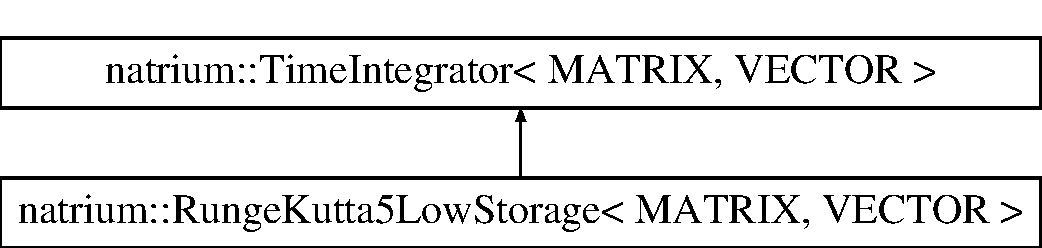
\includegraphics[height=2.000000cm]{classnatrium_1_1RungeKutta5LowStorage}
\end{center}
\end{figure}
\subsection*{\-Public \-Member \-Functions}
\begin{DoxyCompactItemize}
\item 
\hypertarget{classnatrium_1_1RungeKutta5LowStorage_adcb00ef16369158a395ecb54e5d5f91e}{\hyperlink{classnatrium_1_1RungeKutta5LowStorage_adcb00ef16369158a395ecb54e5d5f91e}{\-Runge\-Kutta5\-Low\-Storage} ()}\label{classnatrium_1_1RungeKutta5LowStorage_adcb00ef16369158a395ecb54e5d5f91e}

\begin{DoxyCompactList}\small\item\em constructor \end{DoxyCompactList}\item 
\hypertarget{classnatrium_1_1RungeKutta5LowStorage_a0d0e4591d2b671f450029bb3ba3053de}{virtual \hyperlink{classnatrium_1_1RungeKutta5LowStorage_a0d0e4591d2b671f450029bb3ba3053de}{$\sim$\-Runge\-Kutta5\-Low\-Storage} ()}\label{classnatrium_1_1RungeKutta5LowStorage_a0d0e4591d2b671f450029bb3ba3053de}

\begin{DoxyCompactList}\small\item\em destructor \end{DoxyCompactList}\end{DoxyCompactItemize}


\subsection{\-Detailed \-Description}
\-Implementation of the fifth-\/order \-Runge-\/\-Kutta time integration scheme with low storage consumption. 

\begin{DoxyNote}{\-Note}
\-The scheme is described in \-Min and \-Lee (2011)\-: \-A spectral-\/element discontinuous \-Galerkin lattice \-Boltzmann method for nearly incompressible flows, \-J\-C\-P 230 pp. 245-\/259. 
\end{DoxyNote}


\-The documentation for this class was generated from the following files\-:\begin{DoxyCompactItemize}
\item 
/home/kraemer/eclipse\-\_\-workspace/\-N\-A\-Triu\-M/src/timeintegration/\hyperlink{RungeKutta5LowStorage_8h}{\-Runge\-Kutta5\-Low\-Storage.\-h}\item 
/home/kraemer/eclipse\-\_\-workspace/\-N\-A\-Triu\-M/src/timeintegration/\hyperlink{RungeKutta5LowStorage_8cpp}{\-Runge\-Kutta5\-Low\-Storage.\-cpp}\end{DoxyCompactItemize}

\hypertarget{classnatrium_1_1SEDGMinLee}{
\section{natrium::SEDGMinLee$<$ dim $>$ Class Template Reference}
\label{classnatrium_1_1SEDGMinLee}\index{natrium::SEDGMinLee@{natrium::SEDGMinLee}}
}


This class solves the linear advection equations by a scheme which is used, e.g., by Min and Lee (2011): A spectral-\/element discontinuous Galerkin lattice Boltzmann method for nearly incompressible flows, JCP 230 pp. 245-\/259. The advection equations used in the Lattice Boltzmann on unstructured grids are \[ \partial_t f_{\alpha} + e_{\alpha} \partial_x f_{\alpha} = 0,\quad \forall {\alpha} = 1,\dots,Q-1 \] where $ f_{\alpha}(x,t) $ are the particle distribution functions, and $ e_{\alpha} $ are the particle velocities. The discontinuous Galerkin (DG) method turns these PDEs into a large system of ODEs which can then be solved by a time integration scheme. Whereas this class implements the SEDG spatial discretization, the time integration is done by a subclass of \hyperlink{classnatrium_1_1TimeIntegrator}{TimeIntegrator}, e.g. \hyperlink{classnatrium_1_1RungeKutta5LowStorage}{RungeKutta5LowStorage}. In other Finite Element schemes, degrees of freedom can belong to different elements (e.g. at corners of elements). In contrast, DG methods have the degrees of freedom belonging to a single element, which can lead to discontinuities at the element faces. To connect neighbor cells, the integral over the boundary of each cell incorporates the solution on neighbor cells. These contributions are called numerical fluxes. The DG scheme uses the weak formulation of the above equations on quadrilateral elements \$\$: \[ \left( \partial_t f_{\alpha} + \partial_x (e_{\alpha} f_{\alpha}), \Phi \right)_{\Omega_e} = \left(n \left[ e_i f_{\alpha} - F^{\ast}_{\alpha}(f) \right], \Phi \right)_{\partial \Omega_e}. \] In this formulation $ F^{\ast}_{i}(f) $ denotes the numerical fluxes. They can be be calculated as central fluxes or Lax-\/Friedrichs fluxes. Lax-\/Friedrichs is in general more accurate for the advection equation. For detailed information on the fluxes, see the cited paper. For spatial integration a Gauss-\/Lobatto quadrature is used, which has the advantage that the resulting mass matrix M\_\-\{\} = (, )\_\-\{\} is diagonal. This circumvents the solution of a linear equation system. Each advection equation leads to a ODE \[ \partial_t f_{\alpha} = M_{\alpha}^{-1}(- e_{\alpha x} D_{{\alpha}x} - e_{{\alpha}y} D_{{\alpha}y} + R_{\alpha}) f_{\alpha} + B_i f_{{\alpha}^{\ast}} + b_{\alpha}.\] Altogether, for the example of the \hyperlink{classnatrium_1_1D2Q9}{D2Q9}, the system becomes \[ \partial_t f_{1,\dots,Q} = \left( \matrix{ L_1 & 0 & B_1 & 0 & 0 & 0 & 0 & 0 \cr 0 & L_2 & 0 & B_2 & 0 & 0 & 0 & 0 \cr B_3 & 0 & L_3 & 0 & 0 & 0 & 0 & 0 \cr 0 & B_4 & 0 & L_4 & 0 & 0 & 0 & 0 \cr 0 & 0 & 0 & 0 & L_5 & 0 & B_5 & 0 \cr 0 & 0 & 0 & 0 & 0 & L_6 & 0 & B_6\cr 0 & 0 & 0 & 0 & B_7 & 0 & L_7 & 0 \cr 0 & 0 & 0 & 0 & 0 & B_8 & 0 & L_8 } \right) f_{1,\dots,Q} + \left( \matrix{ b_1 \cr b_2 \cr b_3 \cr b_4 \cr b_5 \cr b_6 \cr b_7 \cr b_8 }\right), \] where $ L_{\alpha} = M_{\alpha}^{-1}(- e_{{\alpha}x} D_{{\alpha}x} - e_{{\alpha}y} D_{{\alpha}y} + R_{\alpha}) $.  


{\ttfamily \#include $<$SEDGMinLee.h$>$}Inheritance diagram for natrium::SEDGMinLee$<$ dim $>$::\begin{figure}[H]
\begin{center}
\leavevmode
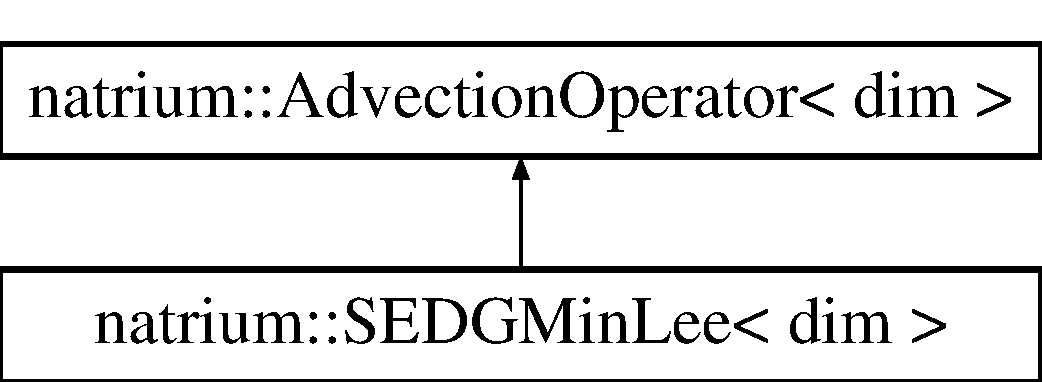
\includegraphics[height=2cm]{classnatrium_1_1SEDGMinLee}
\end{center}
\end{figure}
\subsection*{Public Member Functions}
\begin{DoxyCompactItemize}
\item 
\hyperlink{classnatrium_1_1SEDGMinLee_a6010ff397c7ea56751187084ad6e7ed0}{SEDGMinLee} (shared\_\-ptr$<$ Mesh$<$ dim $>$ $>$ triangulation, shared\_\-ptr$<$ \hyperlink{classnatrium_1_1BoundaryCollection}{BoundaryCollection}$<$ dim $>$ $>$ boundaries, size\_\-t orderOfFiniteElement, shared\_\-ptr$<$ \hyperlink{classnatrium_1_1Stencil}{Stencil} $>$ stencil, string inputDirectory=\char`\"{}\char`\"{}, bool useCentralFlux=false)
\begin{DoxyCompactList}\small\item\em constructor \item\end{DoxyCompactList}\item 
\hypertarget{classnatrium_1_1SEDGMinLee_a6c55a31bc4cb0e314876af7251ad8ce3}{
virtual \hyperlink{classnatrium_1_1SEDGMinLee_a6c55a31bc4cb0e314876af7251ad8ce3}{$\sim$SEDGMinLee} ()}
\label{classnatrium_1_1SEDGMinLee_a6c55a31bc4cb0e314876af7251ad8ce3}

\begin{DoxyCompactList}\small\item\em destructor \item\end{DoxyCompactList}\item 
virtual void \hyperlink{classnatrium_1_1SEDGMinLee_a5fa8b34df3c3bdd9f492a1e555effbe4}{reassemble} ()
\begin{DoxyCompactList}\small\item\em function to (re-\/)assemble linear system \item\end{DoxyCompactList}\item 
\hypertarget{classnatrium_1_1SEDGMinLee_a04707d696f7f466f17e3de055187ecd9}{
virtual void \hyperlink{classnatrium_1_1SEDGMinLee_a04707d696f7f466f17e3de055187ecd9}{stream} ()}
\label{classnatrium_1_1SEDGMinLee_a04707d696f7f466f17e3de055187ecd9}

\begin{DoxyCompactList}\small\item\em make streaming step \item\end{DoxyCompactList}\item 
virtual void \hyperlink{classnatrium_1_1SEDGMinLee_ab3cf80e18230ee7f08f4ed9883b9dadd}{saveCheckpoint} (const string \&directory) const 
\begin{DoxyCompactList}\small\item\em save matrices and status to files \item\end{DoxyCompactList}\item 
\hypertarget{classnatrium_1_1SEDGMinLee_adcf3f6321cbf27f6c540a6c5f21c7cb0}{
virtual const distributed\_\-sparse\_\-block\_\-matrix \& \hyperlink{classnatrium_1_1SEDGMinLee_adcf3f6321cbf27f6c540a6c5f21c7cb0}{getSystemMatrix} () const }
\label{classnatrium_1_1SEDGMinLee_adcf3f6321cbf27f6c540a6c5f21c7cb0}

\begin{DoxyCompactList}\small\item\em get global system matrix \item\end{DoxyCompactList}\item 
\hypertarget{classnatrium_1_1SEDGMinLee_ac1f5ecd80111566dd53804b6db2a1cb3}{
virtual void {\bfseries mapDoFsToSupportPoints} (std::map$<$ dealii::types::global\_\-dof\_\-index, dealii::Point$<$ dim $>$ $>$ \&supportPoints) const }
\label{classnatrium_1_1SEDGMinLee_ac1f5ecd80111566dd53804b6db2a1cb3}

\item 
\hypertarget{classnatrium_1_1SEDGMinLee_a3ffd3d7bc5aae9dbb5a021d7e4913f65}{
virtual const shared\_\-ptr$<$ dealii::DoFHandler$<$ dim $>$ $>$ \& {\bfseries getDoFHandler} () const }
\label{classnatrium_1_1SEDGMinLee_a3ffd3d7bc5aae9dbb5a021d7e4913f65}

\item 
\hypertarget{classnatrium_1_1SEDGMinLee_a10acabaac20a992130e88fb9bd395d31}{
const dealii::BlockSparsityPattern \& {\bfseries getBlockSparsityPattern} () const }
\label{classnatrium_1_1SEDGMinLee_a10acabaac20a992130e88fb9bd395d31}

\item 
const dealii::SparsityPattern \& \hyperlink{classnatrium_1_1SEDGMinLee_ac9392932aaab8186b427b9d12bc64771}{getSparsityPattern} (size\_\-t i) const 
\begin{DoxyCompactList}\small\item\em get sparsity pattern \item\end{DoxyCompactList}\item 
\hypertarget{classnatrium_1_1SEDGMinLee_ab888ac14b8ef33ed706b5d63deea86ae}{
const dealii::MappingQ$<$ dim $>$ \& {\bfseries getMapping} () const }
\label{classnatrium_1_1SEDGMinLee_ab888ac14b8ef33ed706b5d63deea86ae}

\item 
\hypertarget{classnatrium_1_1SEDGMinLee_aec38323cbd34487a73b4f62f0a310ceb}{
virtual const std::map$<$ size\_\-t, size\_\-t $>$ \& {\bfseries getCelldofToQIndex} () const }
\label{classnatrium_1_1SEDGMinLee_aec38323cbd34487a73b4f62f0a310ceb}

\item 
\hypertarget{classnatrium_1_1SEDGMinLee_a8b7d94c90ccfa5e341d854059d883f57}{
const vector$<$ std::map$<$ size\_\-t, size\_\-t $>$ $>$ \& {\bfseries getFacedofToQIndex} () const }
\label{classnatrium_1_1SEDGMinLee_a8b7d94c90ccfa5e341d854059d883f57}

\item 
\hypertarget{classnatrium_1_1SEDGMinLee_a653928dc9f0dd3715389b28196cab7bb}{
const shared\_\-ptr$<$ dealii::QGaussLobatto$<$ dim-\/1 $>$ $>$ \& {\bfseries getFaceQuadrature} () const }
\label{classnatrium_1_1SEDGMinLee_a653928dc9f0dd3715389b28196cab7bb}

\item 
\hypertarget{classnatrium_1_1SEDGMinLee_a7fd488e872e5cf9870be39f07a2dcd74}{
virtual const shared\_\-ptr$<$ dealii::FE\_\-DGQArbitraryNodes$<$ dim $>$ $>$ \& {\bfseries getFe} () const }
\label{classnatrium_1_1SEDGMinLee_a7fd488e872e5cf9870be39f07a2dcd74}

\item 
\hypertarget{classnatrium_1_1SEDGMinLee_a5dac839ef4963af315dba5f201bd763c}{
virtual size\_\-t {\bfseries getNumberOfDoFsPerCell} () const }
\label{classnatrium_1_1SEDGMinLee_a5dac839ef4963af315dba5f201bd763c}

\item 
\hypertarget{classnatrium_1_1SEDGMinLee_a4db0d2b4c857962d5425f755be3daf13}{
virtual const shared\_\-ptr$<$ dealii::QGaussLobatto$<$ dim $>$ $>$ \& {\bfseries getQuadrature} () const }
\label{classnatrium_1_1SEDGMinLee_a4db0d2b4c857962d5425f755be3daf13}

\item 
\hypertarget{classnatrium_1_1SEDGMinLee_a745a65de3ee72a250c0706e6c7fcc361}{
size\_\-t {\bfseries getOrderOfFiniteElement} () const }
\label{classnatrium_1_1SEDGMinLee_a745a65de3ee72a250c0706e6c7fcc361}

\item 
\hypertarget{classnatrium_1_1SEDGMinLee_af667cda1a894340f614da67c0a0ae5da}{
virtual size\_\-t {\bfseries getNumberOfDoFs} () const }
\label{classnatrium_1_1SEDGMinLee_af667cda1a894340f614da67c0a0ae5da}

\item 
\hypertarget{classnatrium_1_1SEDGMinLee_ac4d17489cf8bf5e98bd7bd4e3e32f0d4}{
virtual const distributed\_\-block\_\-vector \& {\bfseries getSystemVector} () const }
\label{classnatrium_1_1SEDGMinLee_ac4d17489cf8bf5e98bd7bd4e3e32f0d4}

\item 
\hypertarget{classnatrium_1_1SEDGMinLee_ab9bdc47144e9e45960ca1bee2593d713}{
{\footnotesize template$<$$>$ }\\void {\bfseries calculateAndDistributeLocalStiffnessMatrix} (size\_\-t alpha, const vector$<$ dealii::FullMatrix$<$ double $>$ $>$ \&derivativeMatrices, dealii::FullMatrix$<$ double $>$ \&systemMatrix, const vector$<$ double $>$ \&inverseLocalMassMatrix, const std::vector$<$ dealii::types::global\_\-dof\_\-index $>$ \&globalDoFs, size\_\-t dofsPerCell)}
\label{classnatrium_1_1SEDGMinLee_ab9bdc47144e9e45960ca1bee2593d713}

\item 
\hypertarget{classnatrium_1_1SEDGMinLee_a7d20a56bbe96969ef037be2a6f47d12d}{
{\footnotesize template$<$$>$ }\\void {\bfseries calculateAndDistributeLocalStiffnessMatrix} (size\_\-t alpha, const vector$<$ dealii::FullMatrix$<$ double $>$ $>$ \&derivativeMatrices, dealii::FullMatrix$<$ double $>$ \&systemMatrix, const vector$<$ double $>$ \&inverseLocalMassMatrix, const std::vector$<$ dealii::types::global\_\-dof\_\-index $>$ \&globalDoFs, size\_\-t dofsPerCell)}
\label{classnatrium_1_1SEDGMinLee_a7d20a56bbe96969ef037be2a6f47d12d}

\end{DoxyCompactItemize}


\subsection{Detailed Description}
\subsubsection*{template$<$size\_\-t dim$>$ class natrium::SEDGMinLee$<$ dim $>$}

This class solves the linear advection equations by a scheme which is used, e.g., by Min and Lee (2011): A spectral-\/element discontinuous Galerkin lattice Boltzmann method for nearly incompressible flows, JCP 230 pp. 245-\/259. The advection equations used in the Lattice Boltzmann on unstructured grids are \[ \partial_t f_{\alpha} + e_{\alpha} \partial_x f_{\alpha} = 0,\quad \forall {\alpha} = 1,\dots,Q-1 \] where $ f_{\alpha}(x,t) $ are the particle distribution functions, and $ e_{\alpha} $ are the particle velocities. The discontinuous Galerkin (DG) method turns these PDEs into a large system of ODEs which can then be solved by a time integration scheme. Whereas this class implements the SEDG spatial discretization, the time integration is done by a subclass of \hyperlink{classnatrium_1_1TimeIntegrator}{TimeIntegrator}, e.g. \hyperlink{classnatrium_1_1RungeKutta5LowStorage}{RungeKutta5LowStorage}. In other Finite Element schemes, degrees of freedom can belong to different elements (e.g. at corners of elements). In contrast, DG methods have the degrees of freedom belonging to a single element, which can lead to discontinuities at the element faces. To connect neighbor cells, the integral over the boundary of each cell incorporates the solution on neighbor cells. These contributions are called numerical fluxes. The DG scheme uses the weak formulation of the above equations on quadrilateral elements \$\$: \[ \left( \partial_t f_{\alpha} + \partial_x (e_{\alpha} f_{\alpha}), \Phi \right)_{\Omega_e} = \left(n \left[ e_i f_{\alpha} - F^{\ast}_{\alpha}(f) \right], \Phi \right)_{\partial \Omega_e}. \] In this formulation $ F^{\ast}_{i}(f) $ denotes the numerical fluxes. They can be be calculated as central fluxes or Lax-\/Friedrichs fluxes. Lax-\/Friedrichs is in general more accurate for the advection equation. For detailed information on the fluxes, see the cited paper. For spatial integration a Gauss-\/Lobatto quadrature is used, which has the advantage that the resulting mass matrix M\_\-\{\} = (, )\_\-\{\} is diagonal. This circumvents the solution of a linear equation system. Each advection equation leads to a ODE \[ \partial_t f_{\alpha} = M_{\alpha}^{-1}(- e_{\alpha x} D_{{\alpha}x} - e_{{\alpha}y} D_{{\alpha}y} + R_{\alpha}) f_{\alpha} + B_i f_{{\alpha}^{\ast}} + b_{\alpha}.\] Altogether, for the example of the \hyperlink{classnatrium_1_1D2Q9}{D2Q9}, the system becomes \[ \partial_t f_{1,\dots,Q} = \left( \matrix{ L_1 & 0 & B_1 & 0 & 0 & 0 & 0 & 0 \cr 0 & L_2 & 0 & B_2 & 0 & 0 & 0 & 0 \cr B_3 & 0 & L_3 & 0 & 0 & 0 & 0 & 0 \cr 0 & B_4 & 0 & L_4 & 0 & 0 & 0 & 0 \cr 0 & 0 & 0 & 0 & L_5 & 0 & B_5 & 0 \cr 0 & 0 & 0 & 0 & 0 & L_6 & 0 & B_6\cr 0 & 0 & 0 & 0 & B_7 & 0 & L_7 & 0 \cr 0 & 0 & 0 & 0 & 0 & B_8 & 0 & L_8 } \right) f_{1,\dots,Q} + \left( \matrix{ b_1 \cr b_2 \cr b_3 \cr b_4 \cr b_5 \cr b_6 \cr b_7 \cr b_8 }\right), \] where $ L_{\alpha} = M_{\alpha}^{-1}(- e_{{\alpha}x} D_{{\alpha}x} - e_{{\alpha}y} D_{{\alpha}y} + R_{\alpha}) $. 
\begin{DoxyTemplParams}{Template Parameters}
\item[{\em dim}]The dimension of the flow (2 or 3). \end{DoxyTemplParams}


\subsection{Constructor \& Destructor Documentation}
\hypertarget{classnatrium_1_1SEDGMinLee_a6010ff397c7ea56751187084ad6e7ed0}{
\index{natrium::SEDGMinLee@{natrium::SEDGMinLee}!SEDGMinLee@{SEDGMinLee}}
\index{SEDGMinLee@{SEDGMinLee}!natrium::SEDGMinLee@{natrium::SEDGMinLee}}
\subsubsection[{SEDGMinLee}]{\setlength{\rightskip}{0pt plus 5cm}template$<$size\_\-t dim$>$ {\bf natrium::SEDGMinLee}$<$ dim $>$::{\bf SEDGMinLee} (shared\_\-ptr$<$ Mesh$<$ dim $>$ $>$ {\em triangulation}, \/  shared\_\-ptr$<$ {\bf BoundaryCollection}$<$ dim $>$ $>$ {\em boundaries}, \/  size\_\-t {\em orderOfFiniteElement}, \/  shared\_\-ptr$<$ {\bf Stencil} $>$ {\em stencil}, \/  string {\em inputDirectory} = {\ttfamily \char`\"{}\char`\"{}}, \/  bool {\em useCentralFlux} = {\ttfamily false})\hspace{0.3cm}{\ttfamily  \mbox{[}inline\mbox{]}}}}
\label{classnatrium_1_1SEDGMinLee_a6010ff397c7ea56751187084ad6e7ed0}


constructor Constructor 
\begin{DoxyParams}{Parameters}
\item[\mbox{$\leftarrow$} {\em triangulation}]The global mesh. \item[\mbox{$\leftarrow$} {\em orderOfFiniteElement}]The number of nodes element and dimension \item[\mbox{$\leftarrow$} {\em stencil}]the DQ model \end{DoxyParams}


\subsection{Member Function Documentation}
\hypertarget{classnatrium_1_1SEDGMinLee_ac9392932aaab8186b427b9d12bc64771}{
\index{natrium::SEDGMinLee@{natrium::SEDGMinLee}!getSparsityPattern@{getSparsityPattern}}
\index{getSparsityPattern@{getSparsityPattern}!natrium::SEDGMinLee@{natrium::SEDGMinLee}}
\subsubsection[{getSparsityPattern}]{\setlength{\rightskip}{0pt plus 5cm}template$<$size\_\-t dim$>$ const dealii::SparsityPattern\& {\bf natrium::SEDGMinLee}$<$ dim $>$::getSparsityPattern (size\_\-t {\em i}) const\hspace{0.3cm}{\ttfamily  \mbox{[}inline\mbox{]}}}}
\label{classnatrium_1_1SEDGMinLee_ac9392932aaab8186b427b9d12bc64771}


get sparsity pattern \begin{DoxyNote}{Note}
not available for trilinos, as trilinos has an internal format for sparsity patterns (Epetra\_\-CrsGraph) 
\end{DoxyNote}
\hypertarget{classnatrium_1_1SEDGMinLee_a5fa8b34df3c3bdd9f492a1e555effbe4}{
\index{natrium::SEDGMinLee@{natrium::SEDGMinLee}!reassemble@{reassemble}}
\index{reassemble@{reassemble}!natrium::SEDGMinLee@{natrium::SEDGMinLee}}
\subsubsection[{reassemble}]{\setlength{\rightskip}{0pt plus 5cm}template$<$size\_\-t dim$>$ template void {\bf natrium::SEDGMinLee}$<$ dim $>$::reassemble ()\hspace{0.3cm}{\ttfamily  \mbox{[}inline, virtual\mbox{]}}}}
\label{classnatrium_1_1SEDGMinLee_a5fa8b34df3c3bdd9f492a1e555effbe4}


function to (re-\/)assemble linear system The template parameter must be made explicit in order for the code to compile. 

Implements \hyperlink{classnatrium_1_1AdvectionOperator_a89c25c3dae9a1e5973cd89fab8c2c052}{natrium::AdvectionOperator$<$ dim $>$}.\hypertarget{classnatrium_1_1SEDGMinLee_ab3cf80e18230ee7f08f4ed9883b9dadd}{
\index{natrium::SEDGMinLee@{natrium::SEDGMinLee}!saveCheckpoint@{saveCheckpoint}}
\index{saveCheckpoint@{saveCheckpoint}!natrium::SEDGMinLee@{natrium::SEDGMinLee}}
\subsubsection[{saveCheckpoint}]{\setlength{\rightskip}{0pt plus 5cm}template$<$size\_\-t dim$>$ template void {\bf natrium::SEDGMinLee}$<$ dim $>$::saveCheckpoint (const string \& {\em directory}) const\hspace{0.3cm}{\ttfamily  \mbox{[}inline, virtual\mbox{]}}}}
\label{classnatrium_1_1SEDGMinLee_ab3cf80e18230ee7f08f4ed9883b9dadd}


save matrices and status to files 
\begin{DoxyParams}{Parameters}
\item[\mbox{$\leftarrow$} {\em directory}]directory to save the matrix files to \end{DoxyParams}

\begin{DoxyExceptions}{Exceptions}
\item[{\em \hyperlink{classnatrium_1_1AdvectionSolverException}{AdvectionSolverException}}]\end{DoxyExceptions}


Implements \hyperlink{classnatrium_1_1AdvectionOperator_aca14260bae100874b0050a2a96d7a564}{natrium::AdvectionOperator$<$ dim $>$}.

The documentation for this class was generated from the following files:\begin{DoxyCompactItemize}
\item 
/mnt/fdrive/akraem3m/workspace/NATriuM/src/library/natrium/advection/\hyperlink{SEDGMinLee_8h}{SEDGMinLee.h}\item 
/mnt/fdrive/akraem3m/workspace/NATriuM/src/library/natrium/advection/\hyperlink{SEDGMinLee_8cpp}{SEDGMinLee.cpp}\end{DoxyCompactItemize}

\hypertarget{classnatrium_1_1SolverConfiguration}{
\section{natrium::SolverConfiguration Class Reference}
\label{classnatrium_1_1SolverConfiguration}\index{natrium::SolverConfiguration@{natrium::SolverConfiguration}}
}


Class that stores the configuration for a CFD simulation based on the Discrete Boltzmann Equation (DBE).  


{\ttfamily \#include $<$SolverConfiguration.h$>$}\subsection*{Public Member Functions}
\begin{DoxyCompactItemize}
\item 
\hypertarget{classnatrium_1_1SolverConfiguration_a9aa7109e2eac9b8a7b424a35509ccdb0}{
\hyperlink{classnatrium_1_1SolverConfiguration_a9aa7109e2eac9b8a7b424a35509ccdb0}{SolverConfiguration} ()}
\label{classnatrium_1_1SolverConfiguration_a9aa7109e2eac9b8a7b424a35509ccdb0}

\begin{DoxyCompactList}\small\item\em Constructor -\/-\/ initializes parameters with their default values. \item\end{DoxyCompactList}\item 
\hyperlink{classnatrium_1_1SolverConfiguration_a062fa86eca607f830540ef4f2c06f0b3}{SolverConfiguration} (const std::string \&XMLfilename)
\begin{DoxyCompactList}\small\item\em Constructor -\/-\/ initializes parameters from an xmlfile. \item\end{DoxyCompactList}\item 
\hypertarget{classnatrium_1_1SolverConfiguration_ac1b521d8c205b8774dbb7c038304336d}{
virtual \hyperlink{classnatrium_1_1SolverConfiguration_ac1b521d8c205b8774dbb7c038304336d}{$\sim$SolverConfiguration} ()}
\label{classnatrium_1_1SolverConfiguration_ac1b521d8c205b8774dbb7c038304336d}

\begin{DoxyCompactList}\small\item\em destructor \item\end{DoxyCompactList}\item 
\hypertarget{classnatrium_1_1SolverConfiguration_a03f1592b0ef8c53729c5bbb9b17e5eb4}{
void \hyperlink{classnatrium_1_1SolverConfiguration_a03f1592b0ef8c53729c5bbb9b17e5eb4}{readFromTextFile} (const std::string \&filename, const bool optional=true, const bool write\_\-stripped\_\-file=false)}
\label{classnatrium_1_1SolverConfiguration_a03f1592b0ef8c53729c5bbb9b17e5eb4}

\begin{DoxyCompactList}\small\item\em wrapper function for ParameterHandler::read\_\-input; directing cerr into a C++-\/Exception \item\end{DoxyCompactList}\item 
\hypertarget{classnatrium_1_1SolverConfiguration_a18c63509007270fa96212fef36a2c172}{
void \hyperlink{classnatrium_1_1SolverConfiguration_a18c63509007270fa96212fef36a2c172}{readFromXMLFile} (const std::string \&filename)}
\label{classnatrium_1_1SolverConfiguration_a18c63509007270fa96212fef36a2c172}

\begin{DoxyCompactList}\small\item\em wrapper function for ParameterHandler::read\_\-input\_\-from\_\-xml; directing cerr into a C++-\/Exception \item\end{DoxyCompactList}\item 
\hypertarget{classnatrium_1_1SolverConfiguration_a90f8fb87f504897d3bbbc746749d2967}{
void \hyperlink{classnatrium_1_1SolverConfiguration_a90f8fb87f504897d3bbbc746749d2967}{isConsistent} ()}
\label{classnatrium_1_1SolverConfiguration_a90f8fb87f504897d3bbbc746749d2967}

\begin{DoxyCompactList}\small\item\em Check if the configuration is consistent. \item\end{DoxyCompactList}\item 
void \hyperlink{classnatrium_1_1SolverConfiguration_a69c009fd87690677b66ab10a000d07f6}{prepareOutputDirectory} ()
\begin{DoxyCompactList}\small\item\em prepare the Output directory \item\end{DoxyCompactList}\item 
void \hyperlink{classnatrium_1_1SolverConfiguration_a368a252965c1b23f7ad6811fdd0adcd4}{checkProblem} (boost::shared\_\-ptr$<$ \hyperlink{classnatrium_1_1ProblemDescription}{ProblemDescription}$<$ 2 $>$ $>$)
\begin{DoxyCompactList}\small\item\em Check if the problem definition is in accordance with the solver configuration. \item\end{DoxyCompactList}\item 
void \hyperlink{classnatrium_1_1SolverConfiguration_a3c66c7b0c5de2bee900835931c50ed5a}{checkProblem} (boost::shared\_\-ptr$<$ \hyperlink{classnatrium_1_1ProblemDescription}{ProblemDescription}$<$ 3 $>$ $>$)
\begin{DoxyCompactList}\small\item\em Check if the problem definition is in accordance with the solver configuration. \item\end{DoxyCompactList}\item 
\hypertarget{classnatrium_1_1SolverConfiguration_aaf32180358f99d78d56b3435dff11a11}{
AdvectionSchemeName {\bfseries getAdvectionScheme} ()}
\label{classnatrium_1_1SolverConfiguration_aaf32180358f99d78d56b3435dff11a11}

\item 
\hypertarget{classnatrium_1_1SolverConfiguration_a4fef165cd5a17247203af08846ec0f31}{
void {\bfseries setAdvectionScheme} (AdvectionSchemeName advectionScheme)}
\label{classnatrium_1_1SolverConfiguration_a4fef165cd5a17247203af08846ec0f31}

\item 
\hypertarget{classnatrium_1_1SolverConfiguration_a90e61c6fa9387a1cbf5943674bf307a8}{
CollisionSchemeName {\bfseries getCollisionScheme} ()}
\label{classnatrium_1_1SolverConfiguration_a90e61c6fa9387a1cbf5943674bf307a8}

\item 
\hypertarget{classnatrium_1_1SolverConfiguration_a5e7241337aa70cbe4b8af29c9cb5cfe8}{
void {\bfseries setCollisionScheme} (CollisionSchemeName collisionScheme)}
\label{classnatrium_1_1SolverConfiguration_a5e7241337aa70cbe4b8af29c9cb5cfe8}

\item 
\hypertarget{classnatrium_1_1SolverConfiguration_a4ebcfcb30f5cb6efb0d9fb3978b9b90f}{
double {\bfseries getBGKSteadyStateGamma} ()}
\label{classnatrium_1_1SolverConfiguration_a4ebcfcb30f5cb6efb0d9fb3978b9b90f}

\item 
\hypertarget{classnatrium_1_1SolverConfiguration_a040a4e68a3ce9502e39deb343586d62b}{
void {\bfseries setBGKSteadyStateGamma} (double gamma)}
\label{classnatrium_1_1SolverConfiguration_a040a4e68a3ce9502e39deb343586d62b}

\item 
\hypertarget{classnatrium_1_1SolverConfiguration_ac1954ee6d225807f947222c437fcd6a4}{
size\_\-t {\bfseries getCommandLineVerbosity} ()}
\label{classnatrium_1_1SolverConfiguration_ac1954ee6d225807f947222c437fcd6a4}

\item 
\hypertarget{classnatrium_1_1SolverConfiguration_a906afb09b544bf2137c0d3bf9214b4a5}{
void {\bfseries setCommandLineVerbosity} (long int commandLineVerbosity)}
\label{classnatrium_1_1SolverConfiguration_a906afb09b544bf2137c0d3bf9214b4a5}

\item 
\hypertarget{classnatrium_1_1SolverConfiguration_a43270017646e2efa400ae84d644ac897}{
bool {\bfseries hasAnalyticSolution} ()}
\label{classnatrium_1_1SolverConfiguration_a43270017646e2efa400ae84d644ac897}

\item 
\hypertarget{classnatrium_1_1SolverConfiguration_ae23ef2513c7b4ed3eacd678e38ff146f}{
void {\bfseries setHasAnalyticSolution} (bool hasAnalyticSolution)}
\label{classnatrium_1_1SolverConfiguration_ae23ef2513c7b4ed3eacd678e38ff146f}

\item 
\hypertarget{classnatrium_1_1SolverConfiguration_afe9fd2087df0ab6066f260bf6bfd03ac}{
InitializationSchemeName {\bfseries getInitializationScheme} ()}
\label{classnatrium_1_1SolverConfiguration_afe9fd2087df0ab6066f260bf6bfd03ac}

\item 
\hypertarget{classnatrium_1_1SolverConfiguration_a4d867b8b8c0c08fc68b95f1a1a52c95d}{
void {\bfseries setInitializationScheme} (InitializationSchemeName initializationScheme)}
\label{classnatrium_1_1SolverConfiguration_a4d867b8b8c0c08fc68b95f1a1a52c95d}

\item 
\hypertarget{classnatrium_1_1SolverConfiguration_aa12123336ffa7489780baa45d99569b1}{
size\_\-t {\bfseries getIterativeInitializationNumberOfIterations} ()}
\label{classnatrium_1_1SolverConfiguration_aa12123336ffa7489780baa45d99569b1}

\item 
\hypertarget{classnatrium_1_1SolverConfiguration_ac4188dce03b129130f153f7028c3f79e}{
void {\bfseries setIterativeInitializationNumberOfIterations} (long int iterativeInitializationNumberOfIterations)}
\label{classnatrium_1_1SolverConfiguration_ac4188dce03b129130f153f7028c3f79e}

\item 
\hypertarget{classnatrium_1_1SolverConfiguration_a966eee9da52af6fbd1f8d5fad2b8427a}{
double {\bfseries getIterativeInitializationResidual} ()}
\label{classnatrium_1_1SolverConfiguration_a966eee9da52af6fbd1f8d5fad2b8427a}

\item 
\hypertarget{classnatrium_1_1SolverConfiguration_ad9551932a38bda46c8ca2ef88a73e754}{
void {\bfseries setIterativeInitializationResidual} (double iterativeInitializationResidual)}
\label{classnatrium_1_1SolverConfiguration_ad9551932a38bda46c8ca2ef88a73e754}

\item 
\hypertarget{classnatrium_1_1SolverConfiguration_a13121a202636553339d5b1f83d196fd7}{
size\_\-t {\bfseries getNumberOfTimeSteps} ()}
\label{classnatrium_1_1SolverConfiguration_a13121a202636553339d5b1f83d196fd7}

\item 
\hypertarget{classnatrium_1_1SolverConfiguration_a50c43893f5c6ed0d73fcccd64f523053}{
void {\bfseries setNumberOfTimeSteps} (long int numberOfTimeSteps)}
\label{classnatrium_1_1SolverConfiguration_a50c43893f5c6ed0d73fcccd64f523053}

\item 
\hypertarget{classnatrium_1_1SolverConfiguration_aa0d9cd3a8d2e6e04fc33e3b4fb8785d9}{
double {\bfseries getSimulationEndTime} ()}
\label{classnatrium_1_1SolverConfiguration_aa0d9cd3a8d2e6e04fc33e3b4fb8785d9}

\item 
\hypertarget{classnatrium_1_1SolverConfiguration_a0d64bd79313ae1aa022d9a2c0e6bc3fd}{
void {\bfseries setSimulationEndTime} (double end\_\-time)}
\label{classnatrium_1_1SolverConfiguration_a0d64bd79313ae1aa022d9a2c0e6bc3fd}

\item 
\hypertarget{classnatrium_1_1SolverConfiguration_a221b5a32cb4cc871536f68a26e14b3c8}{
double {\bfseries getConvergenceThreshold} ()}
\label{classnatrium_1_1SolverConfiguration_a221b5a32cb4cc871536f68a26e14b3c8}

\item 
\hypertarget{classnatrium_1_1SolverConfiguration_a8e7af89ae281933e0f70771ef09147b0}{
void {\bfseries setConvergenceThreshold} (double threshold)}
\label{classnatrium_1_1SolverConfiguration_a8e7af89ae281933e0f70771ef09147b0}

\item 
\hypertarget{classnatrium_1_1SolverConfiguration_a7b7ffc9156ba827ab74ff6f1d7bd9151}{
size\_\-t {\bfseries getOutputCheckpointInterval} ()}
\label{classnatrium_1_1SolverConfiguration_a7b7ffc9156ba827ab74ff6f1d7bd9151}

\item 
\hypertarget{classnatrium_1_1SolverConfiguration_ab7a39dfb46cb1b0c7b54b92700fd7360}{
void {\bfseries setOutputCheckpointInterval} (long int outputCheckpointInterval)}
\label{classnatrium_1_1SolverConfiguration_ab7a39dfb46cb1b0c7b54b92700fd7360}

\item 
\hypertarget{classnatrium_1_1SolverConfiguration_a6c0fb63902a6828c06c48918402375bb}{
size\_\-t {\bfseries getOutputTableInterval} ()}
\label{classnatrium_1_1SolverConfiguration_a6c0fb63902a6828c06c48918402375bb}

\item 
\hypertarget{classnatrium_1_1SolverConfiguration_a207c38e009015be45e74eaa86f9db7ad}{
void {\bfseries setOutputTableInterval} (long int outputTableInterval)}
\label{classnatrium_1_1SolverConfiguration_a207c38e009015be45e74eaa86f9db7ad}

\item 
\hypertarget{classnatrium_1_1SolverConfiguration_a2a0444878a5fb512772e024bc03ec076}{
const std::string {\bfseries getOutputDirectory} ()}
\label{classnatrium_1_1SolverConfiguration_a2a0444878a5fb512772e024bc03ec076}

\item 
\hypertarget{classnatrium_1_1SolverConfiguration_acd249488bb83773514c4d6917b5bfc3a}{
void {\bfseries setOutputDirectory} (const std::string \&outputDirectory)}
\label{classnatrium_1_1SolverConfiguration_acd249488bb83773514c4d6917b5bfc3a}

\item 
\hypertarget{classnatrium_1_1SolverConfiguration_aa7fdb1358469be8faf1cc14c64538927}{
size\_\-t {\bfseries getOutputSolutionInterval} ()}
\label{classnatrium_1_1SolverConfiguration_aa7fdb1358469be8faf1cc14c64538927}

\item 
\hypertarget{classnatrium_1_1SolverConfiguration_ab49c72f19d58f7408eb14ac7fd865b78}{
void {\bfseries setOutputSolutionInterval} (long int outputSolutionInterval)}
\label{classnatrium_1_1SolverConfiguration_ab49c72f19d58f7408eb14ac7fd865b78}

\item 
\hypertarget{classnatrium_1_1SolverConfiguration_a6ca256e404b94f7201ecace9307ef1df}{
bool {\bfseries isRestartAtLastCheckpoint} ()}
\label{classnatrium_1_1SolverConfiguration_a6ca256e404b94f7201ecace9307ef1df}

\item 
\hypertarget{classnatrium_1_1SolverConfiguration_af6077ef11412e53eb16c013b4362410e}{
void {\bfseries setRestartAtLastCheckpoint} (bool restartAtLastCheckpoint)}
\label{classnatrium_1_1SolverConfiguration_af6077ef11412e53eb16c013b4362410e}

\item 
\hypertarget{classnatrium_1_1SolverConfiguration_aecc2a87bc6e50d6e09ea035678478c4f}{
FluxTypeName {\bfseries getSedgFluxType} ()}
\label{classnatrium_1_1SolverConfiguration_aecc2a87bc6e50d6e09ea035678478c4f}

\item 
\hypertarget{classnatrium_1_1SolverConfiguration_a331256f91794e32be618b1162c321bdd}{
void {\bfseries setSedgFluxType} (FluxTypeName sedgFluxType)}
\label{classnatrium_1_1SolverConfiguration_a331256f91794e32be618b1162c321bdd}

\item 
\hypertarget{classnatrium_1_1SolverConfiguration_a1fad5bbbc062b1aad018da73e90033b2}{
size\_\-t {\bfseries getSedgOrderOfFiniteElement} ()}
\label{classnatrium_1_1SolverConfiguration_a1fad5bbbc062b1aad018da73e90033b2}

\item 
\hypertarget{classnatrium_1_1SolverConfiguration_a2a9ab8b6b6dcb47ad4bb85ef06e15dea}{
void {\bfseries setSedgOrderOfFiniteElement} (long int sedgOrderOfFiniteElement)}
\label{classnatrium_1_1SolverConfiguration_a2a9ab8b6b6dcb47ad4bb85ef06e15dea}

\item 
\hypertarget{classnatrium_1_1SolverConfiguration_adb7b45c43f97f0ce2ca288f92a32b577}{
double {\bfseries getStencilScaling} ()}
\label{classnatrium_1_1SolverConfiguration_adb7b45c43f97f0ce2ca288f92a32b577}

\item 
\hypertarget{classnatrium_1_1SolverConfiguration_a1dff19c0a3cc7386bd629dd72e59ac42}{
void {\bfseries setStencilScaling} (double stencilScaling)}
\label{classnatrium_1_1SolverConfiguration_a1dff19c0a3cc7386bd629dd72e59ac42}

\item 
\hypertarget{classnatrium_1_1SolverConfiguration_a962af94c9599c393d8a16d7f5ae04d6c}{
StencilType {\bfseries getStencil} ()}
\label{classnatrium_1_1SolverConfiguration_a962af94c9599c393d8a16d7f5ae04d6c}

\item 
\hypertarget{classnatrium_1_1SolverConfiguration_afa50192447fb027d0250a29b1ea86d1a}{
void {\bfseries setStencil} (StencilType stencil)}
\label{classnatrium_1_1SolverConfiguration_afa50192447fb027d0250a29b1ea86d1a}

\item 
\hypertarget{classnatrium_1_1SolverConfiguration_ac7e6189aaa1b54016993e852999376eb}{
TimeIntegratorName {\bfseries getTimeIntegrator} ()}
\label{classnatrium_1_1SolverConfiguration_ac7e6189aaa1b54016993e852999376eb}

\item 
\hypertarget{classnatrium_1_1SolverConfiguration_ac58399f50e64bc8b0efde5b51e246aeb}{
void {\bfseries setTimeIntegrator} (TimeIntegratorName timeIntegrator)}
\label{classnatrium_1_1SolverConfiguration_ac58399f50e64bc8b0efde5b51e246aeb}

\item 
\hypertarget{classnatrium_1_1SolverConfiguration_a0e2606b5c10964a08e7107dbe079a1ed}{
double {\bfseries getThetaMethodTheta} ()}
\label{classnatrium_1_1SolverConfiguration_a0e2606b5c10964a08e7107dbe079a1ed}

\item 
\hypertarget{classnatrium_1_1SolverConfiguration_acb2153b276dfc0e28bb2cabf8855acd0}{
void {\bfseries setThetaMethodTheta} (double theta)}
\label{classnatrium_1_1SolverConfiguration_acb2153b276dfc0e28bb2cabf8855acd0}

\item 
\hypertarget{classnatrium_1_1SolverConfiguration_a5ba156b86d81572776d8c20b04f21dcc}{
DealIntegratorName {\bfseries getDealIntegrator} ()}
\label{classnatrium_1_1SolverConfiguration_a5ba156b86d81572776d8c20b04f21dcc}

\item 
\hypertarget{classnatrium_1_1SolverConfiguration_acf54eacaa0135343d69a31f0bbc8031c}{
void {\bfseries setDealIntegrator} (DealIntegratorName integrator)}
\label{classnatrium_1_1SolverConfiguration_acf54eacaa0135343d69a31f0bbc8031c}

\item 
\hypertarget{classnatrium_1_1SolverConfiguration_a0678dd0f89508e37c5c555413d5dc258}{
DealSolverName {\bfseries getDealLinearSolver} ()}
\label{classnatrium_1_1SolverConfiguration_a0678dd0f89508e37c5c555413d5dc258}

\item 
\hypertarget{classnatrium_1_1SolverConfiguration_a63ab4a5ff44381dfff6558c030fa3665}{
void {\bfseries setDealLinearSolver} (DealSolverName solver)}
\label{classnatrium_1_1SolverConfiguration_a63ab4a5ff44381dfff6558c030fa3665}

\item 
\hypertarget{classnatrium_1_1SolverConfiguration_a7a017f7078ef42c350efbfca51d9681c}{
void {\bfseries setEmbeddedDealIntegratorParameters} (double coarsen\_\-param, double refine\_\-param, double min\_\-delta, double max\_\-delta, double refine\_\-tol, double coarsen\_\-tol)}
\label{classnatrium_1_1SolverConfiguration_a7a017f7078ef42c350efbfca51d9681c}

\item 
\hypertarget{classnatrium_1_1SolverConfiguration_a0e233c5ac8c6387bf31923700fd95b56}{
double {\bfseries getEmbeddedDealIntegratorCoarsenParameter} ()}
\label{classnatrium_1_1SolverConfiguration_a0e233c5ac8c6387bf31923700fd95b56}

\item 
\hypertarget{classnatrium_1_1SolverConfiguration_a9f8fda7b80e405dab21388cdb0eacbbe}{
double {\bfseries getEmbeddedDealIntegratorRefinementParameter} ()}
\label{classnatrium_1_1SolverConfiguration_a9f8fda7b80e405dab21388cdb0eacbbe}

\item 
\hypertarget{classnatrium_1_1SolverConfiguration_a42688d5882305d75929798685dcd3b0b}{
double {\bfseries getEmbeddedDealIntegratorMinimumTimeStep} ()}
\label{classnatrium_1_1SolverConfiguration_a42688d5882305d75929798685dcd3b0b}

\item 
\hypertarget{classnatrium_1_1SolverConfiguration_a01efc16a1f7c548ef83acdf4bb5bdaf4}{
double {\bfseries getEmbeddedDealIntegratorMaximumTimeStep} ()}
\label{classnatrium_1_1SolverConfiguration_a01efc16a1f7c548ef83acdf4bb5bdaf4}

\item 
\hypertarget{classnatrium_1_1SolverConfiguration_a2c6da5cc4bcfc653c0f3b93b57a4ddf5}{
double {\bfseries getEmbeddedDealIntegratorRefinementTolerance} ()}
\label{classnatrium_1_1SolverConfiguration_a2c6da5cc4bcfc653c0f3b93b57a4ddf5}

\item 
\hypertarget{classnatrium_1_1SolverConfiguration_afedfb3328b78940a7e929214c6d08741}{
double {\bfseries getEmbeddedDealIntegratorCoarsenTolerance} ()}
\label{classnatrium_1_1SolverConfiguration_afedfb3328b78940a7e929214c6d08741}

\item 
\hypertarget{classnatrium_1_1SolverConfiguration_ae446f5d60a09f30a43258a5ec2bebbbf}{
double {\bfseries getTimeStepSize} ()}
\label{classnatrium_1_1SolverConfiguration_ae446f5d60a09f30a43258a5ec2bebbbf}

\item 
\hypertarget{classnatrium_1_1SolverConfiguration_aab0d1b737708c92e83ebe3424b3bed4d}{
void {\bfseries setTimeStepSize} (double timeStepSize)}
\label{classnatrium_1_1SolverConfiguration_aab0d1b737708c92e83ebe3424b3bed4d}

\item 
\hypertarget{classnatrium_1_1SolverConfiguration_ac97dc43684f8a690de0f3e9c132dda02}{
bool {\bfseries isWriteALogFile} ()}
\label{classnatrium_1_1SolverConfiguration_ac97dc43684f8a690de0f3e9c132dda02}

\item 
\hypertarget{classnatrium_1_1SolverConfiguration_a6e50f8fc372b4346ba9f309d5d5f47b3}{
void {\bfseries setWriteALogFile} (bool writeALogFile)}
\label{classnatrium_1_1SolverConfiguration_a6e50f8fc372b4346ba9f309d5d5f47b3}

\item 
\hypertarget{classnatrium_1_1SolverConfiguration_ae4852378b026ccc913732eb8b20eca74}{
bool {\bfseries isSwitchOutputOff} ()}
\label{classnatrium_1_1SolverConfiguration_ae4852378b026ccc913732eb8b20eca74}

\item 
\hypertarget{classnatrium_1_1SolverConfiguration_afcae7f43456c2a127c242b230ea3a8a2}{
void {\bfseries setSwitchOutputOff} (bool switchOutputOff)}
\label{classnatrium_1_1SolverConfiguration_afcae7f43456c2a127c242b230ea3a8a2}

\item 
\hypertarget{classnatrium_1_1SolverConfiguration_a6e41f8ce5da4ecafe2e4326997e79f3d}{
bool {\bfseries isUserInteraction} ()}
\label{classnatrium_1_1SolverConfiguration_a6e41f8ce5da4ecafe2e4326997e79f3d}

\item 
\hypertarget{classnatrium_1_1SolverConfiguration_ad013b9240ee7ae0d5cc43ff5f588c3f3}{
void {\bfseries setUserInteraction} (bool userInteract)}
\label{classnatrium_1_1SolverConfiguration_ad013b9240ee7ae0d5cc43ff5f588c3f3}

\end{DoxyCompactItemize}


\subsection{Detailed Description}
Class that stores the configuration for a CFD simulation based on the Discrete Boltzmann Equation (DBE). \begin{DoxyNote}{Note}
The class is a subclass of dealii::ParameterHandler and functions as a wrapper. 

To integrate new parameter into the framework, you have to declare the paramters in the constructor and write the getter and setter. The setter and getter have to navigate through the sections of the Parameter handler and catch the exceptions thrown by the Parameter handler. Finally you have to update the preprocessor/NATriuM\_\-parameters.xml file, most easily run the UnitTests and copy results/NATriuM\_\-parameters.xml there. The latter file is automatically created according to the declared parameters. Every selection-\/type parameter (e.g. Advection scheme) is implemented as an enum for better handling through the command line. 
\end{DoxyNote}
\begin{Desc}
\item[Examples: ]\par


\hyperlink{step-0_8cpp-example}{step-\/0.cpp}.\end{Desc}


\subsection{Constructor \& Destructor Documentation}
\hypertarget{classnatrium_1_1SolverConfiguration_a062fa86eca607f830540ef4f2c06f0b3}{
\index{natrium::SolverConfiguration@{natrium::SolverConfiguration}!SolverConfiguration@{SolverConfiguration}}
\index{SolverConfiguration@{SolverConfiguration}!natrium::SolverConfiguration@{natrium::SolverConfiguration}}
\subsubsection[{SolverConfiguration}]{\setlength{\rightskip}{0pt plus 5cm}natrium::SolverConfiguration::SolverConfiguration (const std::string \& {\em XMLfilename})}}
\label{classnatrium_1_1SolverConfiguration_a062fa86eca607f830540ef4f2c06f0b3}


Constructor -\/-\/ initializes parameters from an xmlfile. 
\begin{DoxyExceptions}{Exceptions}
\item[{\em \hyperlink{classnatrium_1_1ConfigurationException}{ConfigurationException}}]if the XML file has wrong format \end{DoxyExceptions}


\subsection{Member Function Documentation}
\hypertarget{classnatrium_1_1SolverConfiguration_a3c66c7b0c5de2bee900835931c50ed5a}{
\index{natrium::SolverConfiguration@{natrium::SolverConfiguration}!checkProblem@{checkProblem}}
\index{checkProblem@{checkProblem}!natrium::SolverConfiguration@{natrium::SolverConfiguration}}
\subsubsection[{checkProblem}]{\setlength{\rightskip}{0pt plus 5cm}void natrium::SolverConfiguration::checkProblem (boost::shared\_\-ptr$<$ {\bf ProblemDescription}$<$ 3 $>$ $>$)\hspace{0.3cm}{\ttfamily  \mbox{[}inline\mbox{]}}}}
\label{classnatrium_1_1SolverConfiguration_a3c66c7b0c5de2bee900835931c50ed5a}


Check if the problem definition is in accordance with the solver configuration. 
\begin{DoxyParams}{Parameters}
\item[\mbox{$\leftarrow$} {\em cFDProblem}]Shared pointer to a problem description\end{DoxyParams}

\begin{DoxyExceptions}{Exceptions}
\item[{\em ...}]//TODO implement custom exception \end{DoxyExceptions}
\hypertarget{classnatrium_1_1SolverConfiguration_a368a252965c1b23f7ad6811fdd0adcd4}{
\index{natrium::SolverConfiguration@{natrium::SolverConfiguration}!checkProblem@{checkProblem}}
\index{checkProblem@{checkProblem}!natrium::SolverConfiguration@{natrium::SolverConfiguration}}
\subsubsection[{checkProblem}]{\setlength{\rightskip}{0pt plus 5cm}void natrium::SolverConfiguration::checkProblem (boost::shared\_\-ptr$<$ {\bf ProblemDescription}$<$ 2 $>$ $>$)\hspace{0.3cm}{\ttfamily  \mbox{[}inline\mbox{]}}}}
\label{classnatrium_1_1SolverConfiguration_a368a252965c1b23f7ad6811fdd0adcd4}


Check if the problem definition is in accordance with the solver configuration. 
\begin{DoxyParams}{Parameters}
\item[\mbox{$\leftarrow$} {\em cFDProblem}]Shared pointer to a problem description\end{DoxyParams}

\begin{DoxyExceptions}{Exceptions}
\item[{\em ...}]//TODO implement custom exception \end{DoxyExceptions}
\hypertarget{classnatrium_1_1SolverConfiguration_a69c009fd87690677b66ab10a000d07f6}{
\index{natrium::SolverConfiguration@{natrium::SolverConfiguration}!prepareOutputDirectory@{prepareOutputDirectory}}
\index{prepareOutputDirectory@{prepareOutputDirectory}!natrium::SolverConfiguration@{natrium::SolverConfiguration}}
\subsubsection[{prepareOutputDirectory}]{\setlength{\rightskip}{0pt plus 5cm}void natrium::SolverConfiguration::prepareOutputDirectory ()}}
\label{classnatrium_1_1SolverConfiguration_a69c009fd87690677b66ab10a000d07f6}


prepare the Output directory \begin{DoxyNote}{Note}
If 'User interaction' is enabled, user input is requested in case of possible overwriting 
\end{DoxyNote}

\begin{DoxyExceptions}{Exceptions}
\item[{\em SolverConfigurationError,if}]it was not possible \end{DoxyExceptions}


If not exists, try to create output directory

try to open all files

try to create a single file 

The documentation for this class was generated from the following files:\begin{DoxyCompactItemize}
\item 
/mnt/fdrive/akraem3m/workspace/NATriuM/src/library/natrium/solver/\hyperlink{SolverConfiguration_8h}{SolverConfiguration.h}\item 
/mnt/fdrive/akraem3m/workspace/NATriuM/src/library/natrium/solver/\hyperlink{SolverConfiguration_8cpp}{SolverConfiguration.cpp}\end{DoxyCompactItemize}

\hypertarget{classnatrium_1_1SolverStats}{\section{natrium\-:\-:Solver\-Stats$<$ dim $>$ Class Template Reference}
\label{classnatrium_1_1SolverStats}\index{natrium\-::\-Solver\-Stats$<$ dim $>$@{natrium\-::\-Solver\-Stats$<$ dim $>$}}
}


Container for solver statistics and table file.  




{\ttfamily \#include $<$Solver\-Stats.\-h$>$}

\subsection*{Public Member Functions}
\begin{DoxyCompactItemize}
\item 
\hypertarget{classnatrium_1_1SolverStats_aaa0b74781be83337875982f0a46c67b8}{\hyperlink{classnatrium_1_1SolverStats_aaa0b74781be83337875982f0a46c67b8}{Solver\-Stats} (\hyperlink{classnatrium_1_1CFDSolver}{C\-F\-D\-Solver}$<$ dim $>$ $\ast$cfdsolver, const std\-::string table\-File\-Name=\char`\"{}\char`\"{})}\label{classnatrium_1_1SolverStats_aaa0b74781be83337875982f0a46c67b8}

\begin{DoxyCompactList}\small\item\em Constructor, if second argument is \char`\"{}\char`\"{} (which it is by default), then no output file is created. \end{DoxyCompactList}\item 
\hypertarget{classnatrium_1_1SolverStats_a32c66bc8d05fbd0144dc9023fd17d3a8}{void {\bfseries print\-Header\-Line} ()}\label{classnatrium_1_1SolverStats_a32c66bc8d05fbd0144dc9023fd17d3a8}

\item 
\hypertarget{classnatrium_1_1SolverStats_a15b90f4fa22d7881a0ab868f2e12680b}{void {\bfseries update} ()}\label{classnatrium_1_1SolverStats_a15b90f4fa22d7881a0ab868f2e12680b}

\item 
\hypertarget{classnatrium_1_1SolverStats_a55101045c882c45fe3b46aa236d63604}{void {\bfseries print\-New\-Line} ()}\label{classnatrium_1_1SolverStats_a55101045c882c45fe3b46aa236d63604}

\item 
\hypertarget{classnatrium_1_1SolverStats_acf824edde9e155f0c19c591179fed5eb}{size\-\_\-t {\bfseries get\-Iteration\-Number} () const }\label{classnatrium_1_1SolverStats_acf824edde9e155f0c19c591179fed5eb}

\item 
\hypertarget{classnatrium_1_1SolverStats_a24d2637fa64a779c0f01820ae7e0dfa6}{double {\bfseries get\-Kin\-E} () const }\label{classnatrium_1_1SolverStats_a24d2637fa64a779c0f01820ae7e0dfa6}

\item 
\hypertarget{classnatrium_1_1SolverStats_ac880e86e2e93cafad88fa447ebb641b5}{double {\bfseries get\-Max\-U} () const }\label{classnatrium_1_1SolverStats_ac880e86e2e93cafad88fa447ebb641b5}

\item 
\hypertarget{classnatrium_1_1SolverStats_ae4ab93dfcac8500e41afe4d14b485a3a}{shared\-\_\-ptr$<$ std\-::fstream $>$ {\bfseries get\-Table\-File} () const }\label{classnatrium_1_1SolverStats_ae4ab93dfcac8500e41afe4d14b485a3a}

\item 
\hypertarget{classnatrium_1_1SolverStats_a7eb7473ffe34d624bb8c09666021a6e8}{double {\bfseries get\-Time} () const }\label{classnatrium_1_1SolverStats_a7eb7473ffe34d624bb8c09666021a6e8}

\item 
\hypertarget{classnatrium_1_1SolverStats_ade0d711e048a834547ad32643bc2b529}{bool {\bfseries is\-Up\-To\-Date} () const }\label{classnatrium_1_1SolverStats_ade0d711e048a834547ad32643bc2b529}

\item 
\hypertarget{classnatrium_1_1SolverStats_aedf3ce8027cba3da15c8b28241234c94}{const std\-::string \& {\bfseries get\-Filename} () const }\label{classnatrium_1_1SolverStats_aedf3ce8027cba3da15c8b28241234c94}

\end{DoxyCompactItemize}


\subsection{Detailed Description}
\subsubsection*{template$<$size\-\_\-t dim$>$class natrium\-::\-Solver\-Stats$<$ dim $>$}

Container for solver statistics and table file. 

\begin{DoxyNote}{Note}
As this class is a friend of \hyperlink{classnatrium_1_1CFDSolver}{C\-F\-D\-Solver}, it can access its private attributes 
\end{DoxyNote}


The documentation for this class was generated from the following file\-:\begin{DoxyCompactItemize}
\item 
/home/kraemer/eclipse\-\_\-workspace/\-N\-A\-Triu\-M/src/natrium/solver/Solver\-Stats.\-h\end{DoxyCompactItemize}

\hypertarget{classnatrium_1_1SteadyPeriodicTestFlow2D}{
\section{natrium::SteadyPeriodicTestFlow2D Class Reference}
\label{classnatrium_1_1SteadyPeriodicTestFlow2D}\index{natrium::SteadyPeriodicTestFlow2D@{natrium::SteadyPeriodicTestFlow2D}}
}


Description of a simple Periodic Flow (flow in square domain). The domain is \mbox{[}0,1\mbox{]}$^\wedge$2. The domain consists of 8 x 8 = 64 Elements (contrast to Min and Lee, who have 6 x 6).  


{\ttfamily \#include $<$PeriodicTestFlow2D.h$>$}Inheritance diagram for natrium::SteadyPeriodicTestFlow2D::\begin{figure}[H]
\begin{center}
\leavevmode
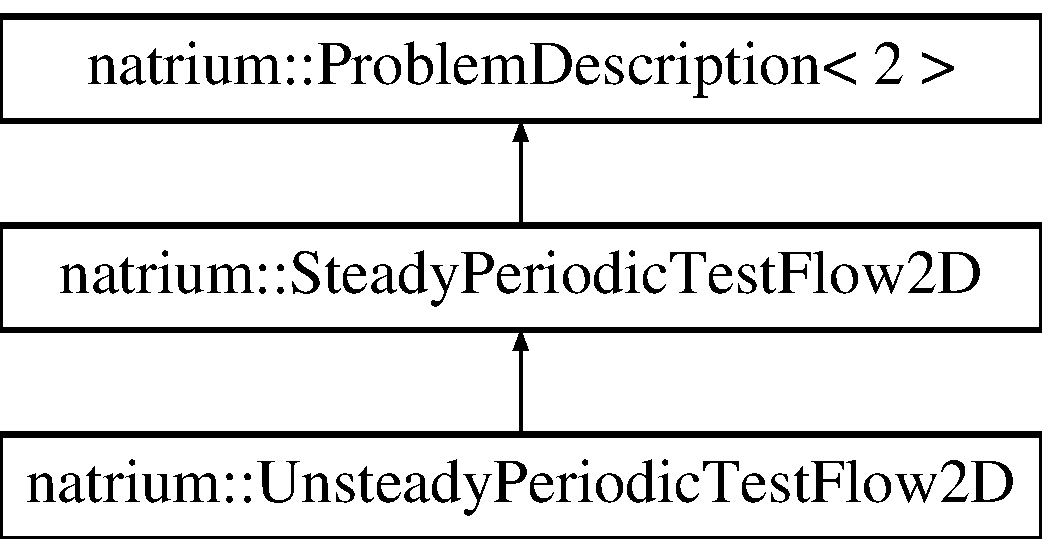
\includegraphics[height=3cm]{classnatrium_1_1SteadyPeriodicTestFlow2D}
\end{center}
\end{figure}
\subsection*{Classes}
\begin{DoxyCompactItemize}
\item 
class \hyperlink{classnatrium_1_1SteadyPeriodicTestFlow2D_1_1InitialVelocity}{InitialVelocity}
\end{DoxyCompactItemize}
\subsection*{Public Member Functions}
\begin{DoxyCompactItemize}
\item 
\hyperlink{classnatrium_1_1SteadyPeriodicTestFlow2D_a7db4598e86b34158612497ea2ff0ca74}{SteadyPeriodicTestFlow2D} (double viscosity, size\_\-t refinementLevel)
\begin{DoxyCompactList}\small\item\em constructor \item\end{DoxyCompactList}\item 
\hypertarget{classnatrium_1_1SteadyPeriodicTestFlow2D_a7344b71a404f2c4bbc73c1c738fdfa22}{
virtual \hyperlink{classnatrium_1_1SteadyPeriodicTestFlow2D_a7344b71a404f2c4bbc73c1c738fdfa22}{$\sim$SteadyPeriodicTestFlow2D} ()}
\label{classnatrium_1_1SteadyPeriodicTestFlow2D_a7344b71a404f2c4bbc73c1c738fdfa22}

\begin{DoxyCompactList}\small\item\em destructor \item\end{DoxyCompactList}\end{DoxyCompactItemize}


\subsection{Detailed Description}
Description of a simple Periodic Flow (flow in square domain). The domain is \mbox{[}0,1\mbox{]}$^\wedge$2. The domain consists of 8 x 8 = 64 Elements (contrast to Min and Lee, who have 6 x 6). 

\subsection{Constructor \& Destructor Documentation}
\hypertarget{classnatrium_1_1SteadyPeriodicTestFlow2D_a7db4598e86b34158612497ea2ff0ca74}{
\index{natrium::SteadyPeriodicTestFlow2D@{natrium::SteadyPeriodicTestFlow2D}!SteadyPeriodicTestFlow2D@{SteadyPeriodicTestFlow2D}}
\index{SteadyPeriodicTestFlow2D@{SteadyPeriodicTestFlow2D}!natrium::SteadyPeriodicTestFlow2D@{natrium::SteadyPeriodicTestFlow2D}}
\subsubsection[{SteadyPeriodicTestFlow2D}]{\setlength{\rightskip}{0pt plus 5cm}natrium::SteadyPeriodicTestFlow2D::SteadyPeriodicTestFlow2D (double {\em viscosity}, \/  size\_\-t {\em refinementLevel})\hspace{0.3cm}{\ttfamily  \mbox{[}inline\mbox{]}}}}
\label{classnatrium_1_1SteadyPeriodicTestFlow2D_a7db4598e86b34158612497ea2ff0ca74}


constructor 

apply boundary values 

The documentation for this class was generated from the following file:\begin{DoxyCompactItemize}
\item 
/mnt/fdrive/akraem3m/workspace/NATriuM/src/test/solver/\hyperlink{PeriodicTestFlow2D_8h}{PeriodicTestFlow2D.h}\end{DoxyCompactItemize}

\hypertarget{classTaylorGreenTest2D}{\section{Taylor\-Green\-Test2\-D Class Reference}
\label{classTaylorGreenTest2D}\index{Taylor\-Green\-Test2\-D@{Taylor\-Green\-Test2\-D}}
}


Description of a Taylor-\/\-Green vortex, a benchmark with only periodic boundaries.  




{\ttfamily \#include $<$Taylor\-Green\-Test2\-D.\-h$>$}

Inheritance diagram for Taylor\-Green\-Test2\-D\-:\begin{figure}[H]
\begin{center}
\leavevmode
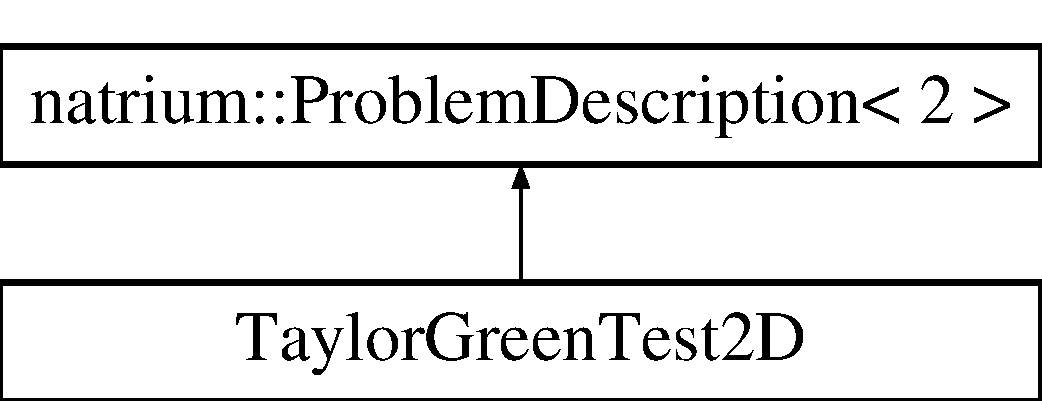
\includegraphics[height=2.000000cm]{classTaylorGreenTest2D}
\end{center}
\end{figure}
\subsection*{Public Member Functions}
\begin{DoxyCompactItemize}
\item 
\hyperlink{classTaylorGreenTest2D_a891500a30b0fae0784496f9c219bd31b}{Taylor\-Green\-Test2\-D} (double viscosity, size\-\_\-t refinement\-Level)
\begin{DoxyCompactList}\small\item\em constructor \end{DoxyCompactList}\item 
\hypertarget{classTaylorGreenTest2D_a393d90458a3415572c3d9bebccdcb662}{virtual \hyperlink{classTaylorGreenTest2D_a393d90458a3415572c3d9bebccdcb662}{$\sim$\-Taylor\-Green\-Test2\-D} ()}\label{classTaylorGreenTest2D_a393d90458a3415572c3d9bebccdcb662}

\begin{DoxyCompactList}\small\item\em destructor \end{DoxyCompactList}\item 
virtual void \hyperlink{classTaylorGreenTest2D_a02adafbe397ef264d790235320b4c4b6}{apply\-Initial\-Densities} (distributed\-\_\-vector \&initial\-Densities, vector$<$ dealii\-::\-Point$<$ 2 $>$ $>$ \&support\-Points) const 
\begin{DoxyCompactList}\small\item\em set initial densities \end{DoxyCompactList}\item 
virtual void \hyperlink{classTaylorGreenTest2D_ad4dfca769ef4500c236dda33d4d9ae54}{apply\-Initial\-Velocities} (vector$<$ distributed\-\_\-vector $>$ \&initial\-Velocities, vector$<$ dealii\-::\-Point$<$ 2 $>$ $>$ \&support\-Points) const 
\begin{DoxyCompactList}\small\item\em set initial velocities \end{DoxyCompactList}\item 
\hypertarget{classTaylorGreenTest2D_a2ae2c4a4ec55242c69a7c9cd60e8bc01}{double \hyperlink{classTaylorGreenTest2D_a2ae2c4a4ec55242c69a7c9cd60e8bc01}{analytic\-Velocity1} (const dealii\-::\-Point$<$ 2 $>$ \&x, double t) const }\label{classTaylorGreenTest2D_a2ae2c4a4ec55242c69a7c9cd60e8bc01}

\begin{DoxyCompactList}\small\item\em analytic solution of the Taylor-\/\-Green vortex, first component of velocity vector \end{DoxyCompactList}\item 
\hypertarget{classTaylorGreenTest2D_af7c07357ef5c57c46218b9c65e45572d}{double \hyperlink{classTaylorGreenTest2D_af7c07357ef5c57c46218b9c65e45572d}{analytic\-Velocity2} (const dealii\-::\-Point$<$ 2 $>$ \&x, double t) const }\label{classTaylorGreenTest2D_af7c07357ef5c57c46218b9c65e45572d}

\begin{DoxyCompactList}\small\item\em analytic solution of the Taylor-\/\-Green vortex, second component of velocity vector \end{DoxyCompactList}\end{DoxyCompactItemize}
\subsection*{Static Public Member Functions}
\begin{DoxyCompactItemize}
\item 
\hypertarget{classTaylorGreenTest2D_a648c0969136540979c37f81d3ab1f1b2}{static void {\bfseries get\-Analytic\-Solution} (double time, distributed\-\_\-vector \&analytic\-Solution1, distributed\-\_\-vector \&analytic\-Solution2, const vector$<$ dealii\-::\-Point$<$ 2 $>$ $>$ \&support\-Points, const \hyperlink{classTaylorGreenTest2D}{Taylor\-Green\-Test2\-D} \&tg\-Vortex)}\label{classTaylorGreenTest2D_a648c0969136540979c37f81d3ab1f1b2}

\end{DoxyCompactItemize}


\subsection{Detailed Description}
Description of a Taylor-\/\-Green vortex, a benchmark with only periodic boundaries. 

\subsection{Constructor \& Destructor Documentation}
\hypertarget{classTaylorGreenTest2D_a891500a30b0fae0784496f9c219bd31b}{\index{Taylor\-Green\-Test2\-D@{Taylor\-Green\-Test2\-D}!Taylor\-Green\-Test2\-D@{Taylor\-Green\-Test2\-D}}
\index{Taylor\-Green\-Test2\-D@{Taylor\-Green\-Test2\-D}!TaylorGreenTest2D@{Taylor\-Green\-Test2\-D}}
\subsubsection[{Taylor\-Green\-Test2\-D}]{\setlength{\rightskip}{0pt plus 5cm}Taylor\-Green\-Test2\-D\-::\-Taylor\-Green\-Test2\-D (
\begin{DoxyParamCaption}
\item[{double}]{viscosity, }
\item[{size\-\_\-t}]{refinement\-Level}
\end{DoxyParamCaption}
)\hspace{0.3cm}{\ttfamily [inline]}}}\label{classTaylorGreenTest2D_a891500a30b0fae0784496f9c219bd31b}


constructor 

apply boundary values 

\subsection{Member Function Documentation}
\hypertarget{classTaylorGreenTest2D_a02adafbe397ef264d790235320b4c4b6}{\index{Taylor\-Green\-Test2\-D@{Taylor\-Green\-Test2\-D}!apply\-Initial\-Densities@{apply\-Initial\-Densities}}
\index{apply\-Initial\-Densities@{apply\-Initial\-Densities}!TaylorGreenTest2D@{Taylor\-Green\-Test2\-D}}
\subsubsection[{apply\-Initial\-Densities}]{\setlength{\rightskip}{0pt plus 5cm}virtual void Taylor\-Green\-Test2\-D\-::apply\-Initial\-Densities (
\begin{DoxyParamCaption}
\item[{distributed\-\_\-vector \&}]{initial\-Densities, }
\item[{vector$<$ dealii\-::\-Point$<$ 2 $>$ $>$ \&}]{support\-Points}
\end{DoxyParamCaption}
) const\hspace{0.3cm}{\ttfamily [inline]}, {\ttfamily [virtual]}}}\label{classTaylorGreenTest2D_a02adafbe397ef264d790235320b4c4b6}


set initial densities 


\begin{DoxyParams}[1]{Parameters}
\mbox{\tt out}  & {\em initial\-Densities} & vector of densities; to be filled \\
\hline
\mbox{\tt in}  & {\em support\-Points} & the coordinates associated with each degree of freedom \\
\hline
\end{DoxyParams}
\hypertarget{classTaylorGreenTest2D_ad4dfca769ef4500c236dda33d4d9ae54}{\index{Taylor\-Green\-Test2\-D@{Taylor\-Green\-Test2\-D}!apply\-Initial\-Velocities@{apply\-Initial\-Velocities}}
\index{apply\-Initial\-Velocities@{apply\-Initial\-Velocities}!TaylorGreenTest2D@{Taylor\-Green\-Test2\-D}}
\subsubsection[{apply\-Initial\-Velocities}]{\setlength{\rightskip}{0pt plus 5cm}virtual void Taylor\-Green\-Test2\-D\-::apply\-Initial\-Velocities (
\begin{DoxyParamCaption}
\item[{vector$<$ distributed\-\_\-vector $>$ \&}]{initial\-Velocities, }
\item[{vector$<$ dealii\-::\-Point$<$ 2 $>$ $>$ \&}]{support\-Points}
\end{DoxyParamCaption}
) const\hspace{0.3cm}{\ttfamily [inline]}, {\ttfamily [virtual]}}}\label{classTaylorGreenTest2D_ad4dfca769ef4500c236dda33d4d9ae54}


set initial velocities 


\begin{DoxyParams}[1]{Parameters}
\mbox{\tt out}  & {\em initial\-Velocities} & vector of velocities; to be filled \\
\hline
\mbox{\tt in}  & {\em support\-Points} & the coordinates associated with each degree of freedom \\
\hline
\end{DoxyParams}


The documentation for this class was generated from the following file\-:\begin{DoxyCompactItemize}
\item 
/home/kraemer/eclipse\-\_\-workspace/\-N\-A\-Triu\-M/src/test/problemdescription/\hyperlink{TaylorGreenTest2D_8h}{Taylor\-Green\-Test2\-D.\-h}\end{DoxyCompactItemize}

\hypertarget{classnatrium_1_1TaylorGreenVortex2D}{
\section{natrium::TaylorGreenVortex2D Class Reference}
\label{classnatrium_1_1TaylorGreenVortex2D}\index{natrium::TaylorGreenVortex2D@{natrium::TaylorGreenVortex2D}}
}


Description of a simple Periodic Flow (flow in square domain). The domain is \mbox{[}0,1\mbox{]}$^\wedge$2. The domain consists of 8 x 8 = 64 Elements (contrast to Min and Lee, who have 6 x 6).  


{\ttfamily \#include $<$TaylorGreenVortex2D.h$>$}Inheritance diagram for natrium::TaylorGreenVortex2D::\begin{figure}[H]
\begin{center}
\leavevmode
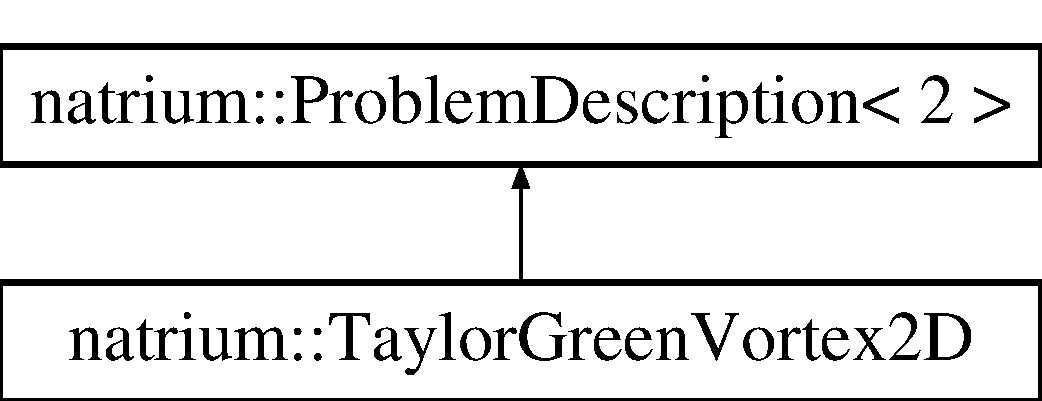
\includegraphics[height=3cm]{classnatrium_1_1TaylorGreenVortex2D}
\end{center}
\end{figure}
\subsection*{Classes}
\begin{DoxyCompactItemize}
\item 
class \hyperlink{classnatrium_1_1TaylorGreenVortex2D_1_1AnalyticDensity}{AnalyticDensity}
\begin{DoxyCompactList}\small\item\em class to describe the y-\/component of the analytic solution \item\end{DoxyCompactList}\item 
class \hyperlink{classnatrium_1_1TaylorGreenVortex2D_1_1AnalyticVelocity}{AnalyticVelocity}
\begin{DoxyCompactList}\small\item\em class to describe the x-\/component of the analytic solution \item\end{DoxyCompactList}\end{DoxyCompactItemize}
\subsection*{Public Member Functions}
\begin{DoxyCompactItemize}
\item 
\hyperlink{classnatrium_1_1TaylorGreenVortex2D_a7f03f55df315b2b2ac1671fa3d07e9df}{TaylorGreenVortex2D} (double viscosity, size\_\-t refinementLevel, double cs=0.57735026919, bool init\_\-rho\_\-analytically=false, double L=2 $\ast$M\_\-PI)
\begin{DoxyCompactList}\small\item\em constructor (with default cs=1/sqrt(3)) \item\end{DoxyCompactList}\item 
\hypertarget{classnatrium_1_1TaylorGreenVortex2D_abb6099f4f9791f7decabb35ccd3dbe49}{
virtual \hyperlink{classnatrium_1_1TaylorGreenVortex2D_abb6099f4f9791f7decabb35ccd3dbe49}{$\sim$TaylorGreenVortex2D} ()}
\label{classnatrium_1_1TaylorGreenVortex2D_abb6099f4f9791f7decabb35ccd3dbe49}

\begin{DoxyCompactList}\small\item\em destructor \item\end{DoxyCompactList}\item 
\hypertarget{classnatrium_1_1TaylorGreenVortex2D_af6f95264a645d97ea207b3e083b8994f}{
virtual void {\bfseries refine} (Mesh$<$ 2 $>$ \&mesh)}
\label{classnatrium_1_1TaylorGreenVortex2D_af6f95264a645d97ea207b3e083b8994f}

\item 
\hypertarget{classnatrium_1_1TaylorGreenVortex2D_a0319526156d349175c2cc7c499a81abe}{
virtual void {\bfseries transform} (Mesh$<$ 2 $>$ \&)}
\label{classnatrium_1_1TaylorGreenVortex2D_a0319526156d349175c2cc7c499a81abe}

\item 
\hypertarget{classnatrium_1_1TaylorGreenVortex2D_a8e58992bc24488b0bc4ea2df4971cd5a}{
virtual bool {\bfseries isCartesian} ()}
\label{classnatrium_1_1TaylorGreenVortex2D_a8e58992bc24488b0bc4ea2df4971cd5a}

\item 
\hypertarget{classnatrium_1_1TaylorGreenVortex2D_ad58ed418e97c541c3d9f8a1b7153bc08}{
void {\bfseries setHorizontalVelocity} (double u)}
\label{classnatrium_1_1TaylorGreenVortex2D_ad58ed418e97c541c3d9f8a1b7153bc08}

\item 
\hypertarget{classnatrium_1_1TaylorGreenVortex2D_a3f47e0968be3cd7ef9ec1cafef8124ab}{
double {\bfseries getHorizontalVelocity} () const }
\label{classnatrium_1_1TaylorGreenVortex2D_a3f47e0968be3cd7ef9ec1cafef8124ab}

\end{DoxyCompactItemize}


\subsection{Detailed Description}
Description of a simple Periodic Flow (flow in square domain). The domain is \mbox{[}0,1\mbox{]}$^\wedge$2. The domain consists of 8 x 8 = 64 Elements (contrast to Min and Lee, who have 6 x 6). 

\subsection{Constructor \& Destructor Documentation}
\hypertarget{classnatrium_1_1TaylorGreenVortex2D_a7f03f55df315b2b2ac1671fa3d07e9df}{
\index{natrium::TaylorGreenVortex2D@{natrium::TaylorGreenVortex2D}!TaylorGreenVortex2D@{TaylorGreenVortex2D}}
\index{TaylorGreenVortex2D@{TaylorGreenVortex2D}!natrium::TaylorGreenVortex2D@{natrium::TaylorGreenVortex2D}}
\subsubsection[{TaylorGreenVortex2D}]{\setlength{\rightskip}{0pt plus 5cm}natrium::TaylorGreenVortex2D::TaylorGreenVortex2D (double {\em viscosity}, \/  size\_\-t {\em refinementLevel}, \/  double {\em cs} = {\ttfamily 0.57735026919}, \/  bool {\em init\_\-rho\_\-analytically} = {\ttfamily false}, \/  double {\em L} = {\ttfamily 2$\ast$M\_\-PI})}}
\label{classnatrium_1_1TaylorGreenVortex2D_a7f03f55df315b2b2ac1671fa3d07e9df}


constructor (with default cs=1/sqrt(3)) 

apply boundary values 

The documentation for this class was generated from the following files:\begin{DoxyCompactItemize}
\item 
/mnt/fdrive/akraem3m/workspace/NATriuM/src/library/natrium/benchmarks/\hyperlink{TaylorGreenVortex2D_8h}{TaylorGreenVortex2D.h}\item 
/mnt/fdrive/akraem3m/workspace/NATriuM/src/library/natrium/benchmarks/\hyperlink{TaylorGreenVortex2D_8cpp}{TaylorGreenVortex2D.cpp}\end{DoxyCompactItemize}

\hypertarget{structnatrium_1_1IntegrationTestCases_1_1TestResult}{
\section{natrium::IntegrationTestCases::TestResult Struct Reference}
\label{structnatrium_1_1IntegrationTestCases_1_1TestResult}\index{natrium::IntegrationTestCases::TestResult@{natrium::IntegrationTestCases::TestResult}}
}
\subsection*{Public Attributes}
\begin{DoxyCompactItemize}
\item 
\hypertarget{structnatrium_1_1IntegrationTestCases_1_1TestResult_a30a8d5f69e4e0d7035a0437f3834b34e}{
size\_\-t {\bfseries id}}
\label{structnatrium_1_1IntegrationTestCases_1_1TestResult_a30a8d5f69e4e0d7035a0437f3834b34e}

\item 
\hypertarget{structnatrium_1_1IntegrationTestCases_1_1TestResult_a2a693e3dab3142fb650e7a6510ff89a7}{
string {\bfseries name}}
\label{structnatrium_1_1IntegrationTestCases_1_1TestResult_a2a693e3dab3142fb650e7a6510ff89a7}

\item 
\hypertarget{structnatrium_1_1IntegrationTestCases_1_1TestResult_af2e7a31b6543fe34f022156030945683}{
string {\bfseries details}}
\label{structnatrium_1_1IntegrationTestCases_1_1TestResult_af2e7a31b6543fe34f022156030945683}

\item 
\hypertarget{structnatrium_1_1IntegrationTestCases_1_1TestResult_a105402717441e46091e7be8106861f58}{
vector$<$ string $>$ {\bfseries quantity}}
\label{structnatrium_1_1IntegrationTestCases_1_1TestResult_a105402717441e46091e7be8106861f58}

\item 
\hypertarget{structnatrium_1_1IntegrationTestCases_1_1TestResult_a10182792d7b4027342ab4368bfa44fb6}{
vector$<$ double $>$ {\bfseries expected}}
\label{structnatrium_1_1IntegrationTestCases_1_1TestResult_a10182792d7b4027342ab4368bfa44fb6}

\item 
\hypertarget{structnatrium_1_1IntegrationTestCases_1_1TestResult_ad69e1b2e302d7b55272e87bc46ca513b}{
vector$<$ double $>$ {\bfseries threshold}}
\label{structnatrium_1_1IntegrationTestCases_1_1TestResult_ad69e1b2e302d7b55272e87bc46ca513b}

\item 
\hypertarget{structnatrium_1_1IntegrationTestCases_1_1TestResult_ac38f2c7a01b0e0501cadf4775bc26572}{
vector$<$ double $>$ {\bfseries outcome}}
\label{structnatrium_1_1IntegrationTestCases_1_1TestResult_ac38f2c7a01b0e0501cadf4775bc26572}

\item 
\hypertarget{structnatrium_1_1IntegrationTestCases_1_1TestResult_a7d0ecf418699d9754fa0a3bed2e34f48}{
boost::shared\_\-ptr$<$ std::stringstream $>$ {\bfseries error\_\-msg}}
\label{structnatrium_1_1IntegrationTestCases_1_1TestResult_a7d0ecf418699d9754fa0a3bed2e34f48}

\item 
\hypertarget{structnatrium_1_1IntegrationTestCases_1_1TestResult_af8b68ac3c5257163877d52c06d599424}{
double {\bfseries time}}
\label{structnatrium_1_1IntegrationTestCases_1_1TestResult_af8b68ac3c5257163877d52c06d599424}

\item 
\hypertarget{structnatrium_1_1IntegrationTestCases_1_1TestResult_abfd745aedfa8bfb6c6f2d93f61294954}{
bool {\bfseries success}}
\label{structnatrium_1_1IntegrationTestCases_1_1TestResult_abfd745aedfa8bfb6c6f2d93f61294954}

\end{DoxyCompactItemize}


The documentation for this struct was generated from the following file:\begin{DoxyCompactItemize}
\item 
/mnt/fdrive/akraem3m/workspace/NATriuM/src/test/integrationtest/IntegrationTestCases.h\end{DoxyCompactItemize}

\hypertarget{classnatrium_1_1ThetaMethod}{\section{natrium\-:\-:Theta\-Method$<$ M\-A\-T\-R\-I\-X, V\-E\-C\-T\-O\-R $>$ Class Template Reference}
\label{classnatrium_1_1ThetaMethod}\index{natrium\-::\-Theta\-Method$<$ M\-A\-T\-R\-I\-X, V\-E\-C\-T\-O\-R $>$@{natrium\-::\-Theta\-Method$<$ M\-A\-T\-R\-I\-X, V\-E\-C\-T\-O\-R $>$}}
}


Implementation of the Theta method for time integration.  




{\ttfamily \#include $<$Theta\-Method.\-h$>$}

Inheritance diagram for natrium\-:\-:Theta\-Method$<$ M\-A\-T\-R\-I\-X, V\-E\-C\-T\-O\-R $>$\-:\begin{figure}[H]
\begin{center}
\leavevmode
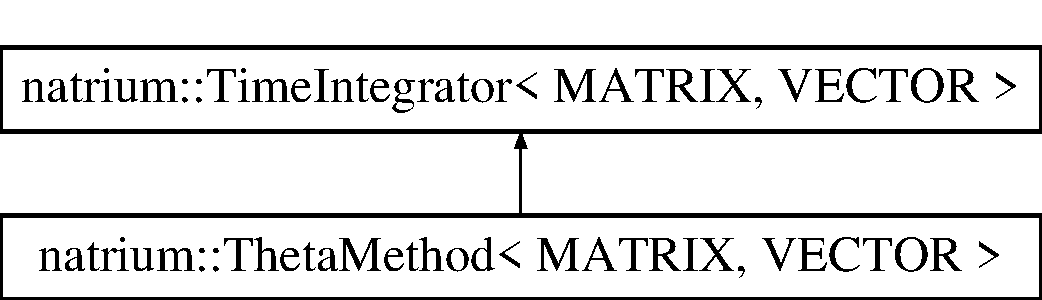
\includegraphics[height=2.000000cm]{classnatrium_1_1ThetaMethod}
\end{center}
\end{figure}
\subsection*{Public Member Functions}
\begin{DoxyCompactItemize}
\item 
\hyperlink{classnatrium_1_1ThetaMethod_a30c8135385f1612ab8e8e7dd8ad21e42}{Theta\-Method} (double time\-Step\-Size, size\-\_\-t problem\-Size, double theta)
\begin{DoxyCompactList}\small\item\em Constructor. \end{DoxyCompactList}\item 
\hyperlink{classnatrium_1_1ThetaMethod_ae5cd52ec9564393a9a14296262ae0512}{Theta\-Method} (double time\-Step\-Size, size\-\_\-t problem\-Size, size\-\_\-t number\-Of\-Blocks, double theta)
\begin{DoxyCompactList}\small\item\em Constructor. \end{DoxyCompactList}\item 
\hypertarget{classnatrium_1_1ThetaMethod_ac742c678ab9674722295585f10d27279}{virtual \hyperlink{classnatrium_1_1ThetaMethod_ac742c678ab9674722295585f10d27279}{$\sim$\-Theta\-Method} ()}\label{classnatrium_1_1ThetaMethod_ac742c678ab9674722295585f10d27279}

\begin{DoxyCompactList}\small\item\em destructor \end{DoxyCompactList}\item 
\hypertarget{classnatrium_1_1ThetaMethod_ae16bd6a1f7f10b161c10909ad6a8744c}{void \hyperlink{classnatrium_1_1ThetaMethod_ae16bd6a1f7f10b161c10909ad6a8744c}{step} (V\-E\-C\-T\-O\-R \&vector, const M\-A\-T\-R\-I\-X \&system\-Matrix, const V\-E\-C\-T\-O\-R \&system\-Vector)}\label{classnatrium_1_1ThetaMethod_ae16bd6a1f7f10b161c10909ad6a8744c}

\begin{DoxyCompactList}\small\item\em One time step of the theta method. \end{DoxyCompactList}\item 
\hypertarget{classnatrium_1_1ThetaMethod_af747ecc6907946598f01eca741a57dae}{{\footnotesize template$<$$>$ }\\{\bfseries Theta\-Method} (double time\-Step\-Size, size\-\_\-t problem\-Size, size\-\_\-t number\-Of\-Blocks, double theta)}\label{classnatrium_1_1ThetaMethod_af747ecc6907946598f01eca741a57dae}

\end{DoxyCompactItemize}


\subsection{Detailed Description}
\subsubsection*{template$<$class M\-A\-T\-R\-I\-X, class V\-E\-C\-T\-O\-R$>$class natrium\-::\-Theta\-Method$<$ M\-A\-T\-R\-I\-X, V\-E\-C\-T\-O\-R $>$}

Implementation of the Theta method for time integration. 

\subsection{Constructor \& Destructor Documentation}
\hypertarget{classnatrium_1_1ThetaMethod_a30c8135385f1612ab8e8e7dd8ad21e42}{\index{natrium\-::\-Theta\-Method@{natrium\-::\-Theta\-Method}!Theta\-Method@{Theta\-Method}}
\index{Theta\-Method@{Theta\-Method}!natrium::ThetaMethod@{natrium\-::\-Theta\-Method}}
\subsubsection[{Theta\-Method}]{\setlength{\rightskip}{0pt plus 5cm}template$<$class M\-A\-T\-R\-I\-X , class V\-E\-C\-T\-O\-R $>$ template {\bf natrium\-::\-Theta\-Method}$<$ M\-A\-T\-R\-I\-X, V\-E\-C\-T\-O\-R $>$\-::{\bf Theta\-Method} (
\begin{DoxyParamCaption}
\item[{double}]{time\-Step\-Size, }
\item[{size\-\_\-t}]{problem\-Size, }
\item[{double}]{theta}
\end{DoxyParamCaption}
)}}\label{classnatrium_1_1ThetaMethod_a30c8135385f1612ab8e8e7dd8ad21e42}


Constructor. 


\begin{DoxyParams}{Parameters}
{\em time\-Step\-Size} & The initial time step size \\
\hline
{\em problem\-Size} & the number of degrees of freedom \\
\hline
{\em theta} & theta = 0\-: Explicit Euler, theta = 1\-: implicit Euler, theta = 0.\-5\-: Crank-\/\-Nicholson. \\
\hline
\end{DoxyParams}
\hypertarget{classnatrium_1_1ThetaMethod_ae5cd52ec9564393a9a14296262ae0512}{\index{natrium\-::\-Theta\-Method@{natrium\-::\-Theta\-Method}!Theta\-Method@{Theta\-Method}}
\index{Theta\-Method@{Theta\-Method}!natrium::ThetaMethod@{natrium\-::\-Theta\-Method}}
\subsubsection[{Theta\-Method}]{\setlength{\rightskip}{0pt plus 5cm}template$<$class M\-A\-T\-R\-I\-X , class V\-E\-C\-T\-O\-R $>$ {\bf natrium\-::\-Theta\-Method}$<$ M\-A\-T\-R\-I\-X, V\-E\-C\-T\-O\-R $>$\-::{\bf Theta\-Method} (
\begin{DoxyParamCaption}
\item[{double}]{time\-Step\-Size, }
\item[{size\-\_\-t}]{problem\-Size, }
\item[{size\-\_\-t}]{number\-Of\-Blocks, }
\item[{double}]{theta}
\end{DoxyParamCaption}
)}}\label{classnatrium_1_1ThetaMethod_ae5cd52ec9564393a9a14296262ae0512}


Constructor. 


\begin{DoxyParams}{Parameters}
{\em time\-Step\-Size} & The initial time step size \\
\hline
{\em problem\-Size} & the number of degrees of freedom \\
\hline
{\em theta} & theta = 0\-: Explicit Euler, theta = 1\-: implicit Euler, theta = 0.\-5\-: Crank-\/\-Nicholson. \\
\hline
\end{DoxyParams}


The documentation for this class was generated from the following files\-:\begin{DoxyCompactItemize}
\item 
/home/kraemer/eclipse\-\_\-workspace/\-N\-A\-Triu\-M/src/natrium/timeintegration/\hyperlink{ThetaMethod_8h}{Theta\-Method.\-h}\item 
/home/kraemer/eclipse\-\_\-workspace/\-N\-A\-Triu\-M/src/natrium/timeintegration/\hyperlink{ThetaMethod_8cpp}{Theta\-Method.\-cpp}\end{DoxyCompactItemize}

\hypertarget{classnatrium_1_1TimeIntegrator}{\section{natrium\-:\-:Time\-Integrator$<$ M\-A\-T\-R\-I\-X, V\-E\-C\-T\-O\-R $>$ Class Template Reference}
\label{classnatrium_1_1TimeIntegrator}\index{natrium\-::\-Time\-Integrator$<$ M\-A\-T\-R\-I\-X, V\-E\-C\-T\-O\-R $>$@{natrium\-::\-Time\-Integrator$<$ M\-A\-T\-R\-I\-X, V\-E\-C\-T\-O\-R $>$}}
}


Abstract class for time integration (solution of ordinary differential equations (O\-D\-E)).  




{\ttfamily \#include $<$Time\-Integrator.\-h$>$}

Inheritance diagram for natrium\-:\-:Time\-Integrator$<$ M\-A\-T\-R\-I\-X, V\-E\-C\-T\-O\-R $>$\-:\begin{figure}[H]
\begin{center}
\leavevmode
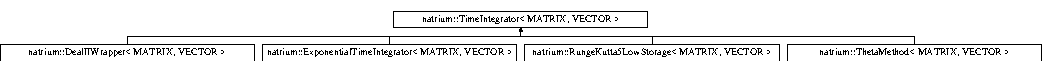
\includegraphics[height=1.666667cm]{classnatrium_1_1TimeIntegrator}
\end{center}
\end{figure}
\subsection*{Public Member Functions}
\begin{DoxyCompactItemize}
\item 
\hypertarget{classnatrium_1_1TimeIntegrator_a420ea9baabf0839bc8ecb5f5e02ce95b}{\hyperlink{classnatrium_1_1TimeIntegrator_a420ea9baabf0839bc8ecb5f5e02ce95b}{Time\-Integrator} (double time\-Step\-Size)}\label{classnatrium_1_1TimeIntegrator_a420ea9baabf0839bc8ecb5f5e02ce95b}

\begin{DoxyCompactList}\small\item\em constructor \end{DoxyCompactList}\item 
\hypertarget{classnatrium_1_1TimeIntegrator_a8795d06c5322b72a5a2a1f30aa7a051d}{virtual \hyperlink{classnatrium_1_1TimeIntegrator_a8795d06c5322b72a5a2a1f30aa7a051d}{$\sim$\-Time\-Integrator} ()}\label{classnatrium_1_1TimeIntegrator_a8795d06c5322b72a5a2a1f30aa7a051d}

\begin{DoxyCompactList}\small\item\em destructor \end{DoxyCompactList}\item 
\hypertarget{classnatrium_1_1TimeIntegrator_a6e763133e114cdd758307ca30b65f161}{double {\bfseries get\-Time\-Step\-Size} () const }\label{classnatrium_1_1TimeIntegrator_a6e763133e114cdd758307ca30b65f161}

\item 
\hypertarget{classnatrium_1_1TimeIntegrator_a18592866e946c63ab1595d3ab688ea6b}{void {\bfseries set\-Time\-Step\-Size} (double time\-Step\-Size)}\label{classnatrium_1_1TimeIntegrator_a18592866e946c63ab1595d3ab688ea6b}

\item 
\hypertarget{classnatrium_1_1TimeIntegrator_a09e1ad9254abec537cda42b1d2fb83e6}{virtual void \hyperlink{classnatrium_1_1TimeIntegrator_a09e1ad9254abec537cda42b1d2fb83e6}{step} (V\-E\-C\-T\-O\-R \&vector, const M\-A\-T\-R\-I\-X \&system\-Matrix, const V\-E\-C\-T\-O\-R \&system\-Vector)=0}\label{classnatrium_1_1TimeIntegrator_a09e1ad9254abec537cda42b1d2fb83e6}

\begin{DoxyCompactList}\small\item\em make one time integration step on vector using the system matrix \end{DoxyCompactList}\end{DoxyCompactItemize}


\subsection{Detailed Description}
\subsubsection*{template$<$class M\-A\-T\-R\-I\-X, class V\-E\-C\-T\-O\-R$>$class natrium\-::\-Time\-Integrator$<$ M\-A\-T\-R\-I\-X, V\-E\-C\-T\-O\-R $>$}

Abstract class for time integration (solution of ordinary differential equations (O\-D\-E)). 

\begin{DoxyNote}{Note}
The O\-D\-Es arise from the space discretization of the D\-B\-E, which is basically a partial differential equation (P\-D\-E). By application of a space discretization scheme (like discontinuous Galerkin or standard F\-E\-M methods) the space derivatives in the P\-D\-E are replaced with arithmetic expressions. The only remaining derivative is then the time derivative, which makes the equation an O\-D\-E. The latter can be solved using classical time integration methods like Runge-\/\-Kutta or Adams-\/\-Moulton. 
\end{DoxyNote}


The documentation for this class was generated from the following files\-:\begin{DoxyCompactItemize}
\item 
/home/kraemer/eclipse\-\_\-workspace/\-N\-A\-Triu\-M/src/natrium/timeintegration/\hyperlink{TimeIntegrator_8h}{Time\-Integrator.\-h}\item 
/home/kraemer/eclipse\-\_\-workspace/\-N\-A\-Triu\-M/src/natrium/timeintegration/\hyperlink{TimeIntegrator_8cpp}{Time\-Integrator.\-cpp}\end{DoxyCompactItemize}

\hypertarget{classnatrium_1_1UnsteadyPeriodicTestFlow2D}{\section{natrium\-:\-:Unsteady\-Periodic\-Test\-Flow2\-D Class Reference}
\label{classnatrium_1_1UnsteadyPeriodicTestFlow2D}\index{natrium\-::\-Unsteady\-Periodic\-Test\-Flow2\-D@{natrium\-::\-Unsteady\-Periodic\-Test\-Flow2\-D}}
}
Inheritance diagram for natrium\-:\-:Unsteady\-Periodic\-Test\-Flow2\-D\-:\begin{figure}[H]
\begin{center}
\leavevmode
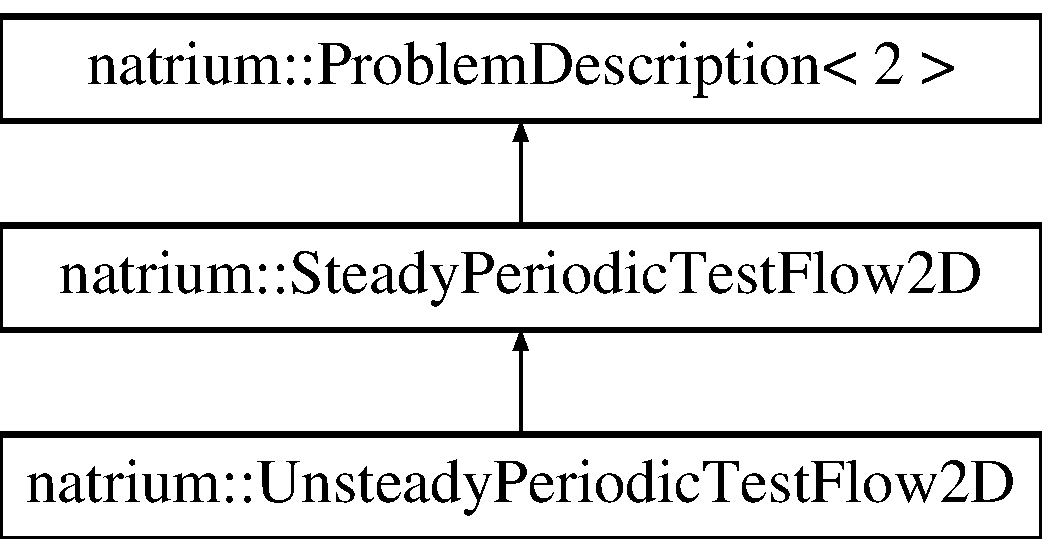
\includegraphics[height=3.000000cm]{classnatrium_1_1UnsteadyPeriodicTestFlow2D}
\end{center}
\end{figure}
\subsection*{Public Member Functions}
\begin{DoxyCompactItemize}
\item 
\hypertarget{classnatrium_1_1UnsteadyPeriodicTestFlow2D_a3a513d06c9018e78041cf8179ef2d80f}{\hyperlink{classnatrium_1_1UnsteadyPeriodicTestFlow2D_a3a513d06c9018e78041cf8179ef2d80f}{Unsteady\-Periodic\-Test\-Flow2\-D} (double viscosity, size\-\_\-t refinement\-Level)}\label{classnatrium_1_1UnsteadyPeriodicTestFlow2D_a3a513d06c9018e78041cf8179ef2d80f}

\begin{DoxyCompactList}\small\item\em constructor \end{DoxyCompactList}\item 
\hypertarget{classnatrium_1_1UnsteadyPeriodicTestFlow2D_aa91ea175e2993bf00f8a48fded987c54}{virtual \hyperlink{classnatrium_1_1UnsteadyPeriodicTestFlow2D_aa91ea175e2993bf00f8a48fded987c54}{$\sim$\-Unsteady\-Periodic\-Test\-Flow2\-D} ()}\label{classnatrium_1_1UnsteadyPeriodicTestFlow2D_aa91ea175e2993bf00f8a48fded987c54}

\begin{DoxyCompactList}\small\item\em destructor \end{DoxyCompactList}\item 
virtual void \hyperlink{classnatrium_1_1UnsteadyPeriodicTestFlow2D_a089ab3cde76dfade1eb8705051af123f}{apply\-Initial\-Densities} (distributed\-\_\-vector \&initial\-Densities, const vector$<$ dealii\-::\-Point$<$ 2 $>$ $>$ \&support\-Points) const 
\begin{DoxyCompactList}\small\item\em set initial densities \end{DoxyCompactList}\item 
virtual void \hyperlink{classnatrium_1_1UnsteadyPeriodicTestFlow2D_a5755fda1ff3726ffc543cf86b618d71e}{apply\-Initial\-Velocities} (vector$<$ distributed\-\_\-vector $>$ \&initial\-Velocities, const vector$<$ dealii\-::\-Point$<$ 2 $>$ $>$ \&support\-Points) const 
\begin{DoxyCompactList}\small\item\em set initial velocities \end{DoxyCompactList}\end{DoxyCompactItemize}


\subsection{Member Function Documentation}
\hypertarget{classnatrium_1_1UnsteadyPeriodicTestFlow2D_a089ab3cde76dfade1eb8705051af123f}{\index{natrium\-::\-Unsteady\-Periodic\-Test\-Flow2\-D@{natrium\-::\-Unsteady\-Periodic\-Test\-Flow2\-D}!apply\-Initial\-Densities@{apply\-Initial\-Densities}}
\index{apply\-Initial\-Densities@{apply\-Initial\-Densities}!natrium::UnsteadyPeriodicTestFlow2D@{natrium\-::\-Unsteady\-Periodic\-Test\-Flow2\-D}}
\subsubsection[{apply\-Initial\-Densities}]{\setlength{\rightskip}{0pt plus 5cm}virtual void natrium\-::\-Unsteady\-Periodic\-Test\-Flow2\-D\-::apply\-Initial\-Densities (
\begin{DoxyParamCaption}
\item[{distributed\-\_\-vector \&}]{initial\-Densities, }
\item[{const vector$<$ dealii\-::\-Point$<$ 2 $>$ $>$ \&}]{support\-Points}
\end{DoxyParamCaption}
) const\hspace{0.3cm}{\ttfamily [inline]}, {\ttfamily [virtual]}}}\label{classnatrium_1_1UnsteadyPeriodicTestFlow2D_a089ab3cde76dfade1eb8705051af123f}


set initial densities 


\begin{DoxyParams}[1]{Parameters}
\mbox{\tt out}  & {\em initial\-Densities} & vector of densities; to be filled \\
\hline
\mbox{\tt in}  & {\em support\-Points} & the coordinates associated with each degree of freedom \\
\hline
\end{DoxyParams}


Reimplemented from \hyperlink{classnatrium_1_1SteadyPeriodicTestFlow2D_a29474cd6d454c3f600693ae2c362cba2}{natrium\-::\-Steady\-Periodic\-Test\-Flow2\-D}.

\hypertarget{classnatrium_1_1UnsteadyPeriodicTestFlow2D_a5755fda1ff3726ffc543cf86b618d71e}{\index{natrium\-::\-Unsteady\-Periodic\-Test\-Flow2\-D@{natrium\-::\-Unsteady\-Periodic\-Test\-Flow2\-D}!apply\-Initial\-Velocities@{apply\-Initial\-Velocities}}
\index{apply\-Initial\-Velocities@{apply\-Initial\-Velocities}!natrium::UnsteadyPeriodicTestFlow2D@{natrium\-::\-Unsteady\-Periodic\-Test\-Flow2\-D}}
\subsubsection[{apply\-Initial\-Velocities}]{\setlength{\rightskip}{0pt plus 5cm}virtual void natrium\-::\-Unsteady\-Periodic\-Test\-Flow2\-D\-::apply\-Initial\-Velocities (
\begin{DoxyParamCaption}
\item[{vector$<$ distributed\-\_\-vector $>$ \&}]{initial\-Velocities, }
\item[{const vector$<$ dealii\-::\-Point$<$ 2 $>$ $>$ \&}]{support\-Points}
\end{DoxyParamCaption}
) const\hspace{0.3cm}{\ttfamily [inline]}, {\ttfamily [virtual]}}}\label{classnatrium_1_1UnsteadyPeriodicTestFlow2D_a5755fda1ff3726ffc543cf86b618d71e}


set initial velocities 


\begin{DoxyParams}[1]{Parameters}
\mbox{\tt out}  & {\em initial\-Velocities} & vector of velocities; to be filled \\
\hline
\mbox{\tt in}  & {\em support\-Points} & the coordinates associated with each degree of freedom \\
\hline
\end{DoxyParams}


Reimplemented from \hyperlink{classnatrium_1_1SteadyPeriodicTestFlow2D_ae0b3291a91029f62b41fd96a128f645a}{natrium\-::\-Steady\-Periodic\-Test\-Flow2\-D}.



The documentation for this class was generated from the following file\-:\begin{DoxyCompactItemize}
\item 
/home/kraemer/eclipse\-\_\-workspace/\-N\-A\-Triu\-M/src/test/solver/\hyperlink{PeriodicTestFlow2D_8h}{Periodic\-Test\-Flow2\-D.\-h}\end{DoxyCompactItemize}

\hypertarget{classWallTestDomain2D}{
\section{WallTestDomain2D Class Reference}
\label{classWallTestDomain2D}\index{WallTestDomain2D@{WallTestDomain2D}}
}


Description of a simple Flow with wall boundaries (flow in square domain). The domain is \mbox{[}0,1\mbox{]}$^\wedge$2. The domain consists of 4 elements.  


{\ttfamily \#include $<$WallTestDomain2D.h$>$}Inheritance diagram for WallTestDomain2D::\begin{figure}[H]
\begin{center}
\leavevmode
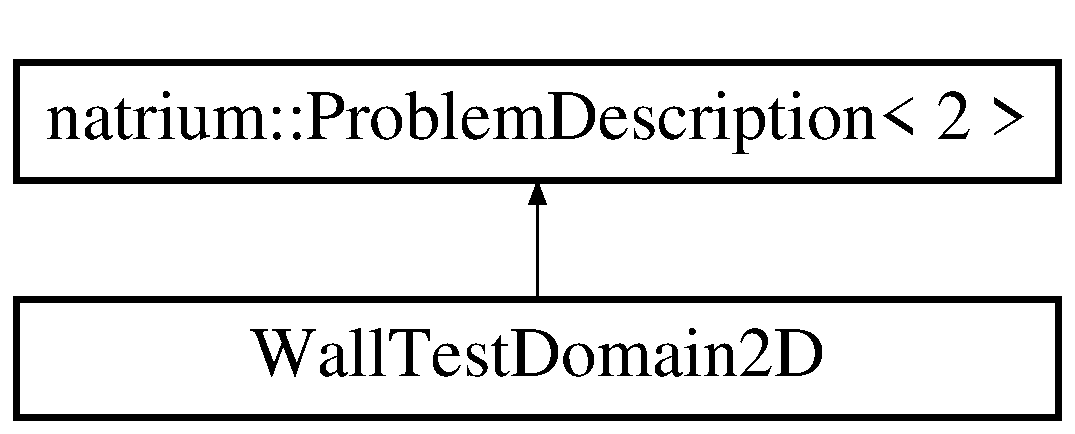
\includegraphics[height=2cm]{classWallTestDomain2D}
\end{center}
\end{figure}
\subsection*{Public Member Functions}
\begin{DoxyCompactItemize}
\item 
\hyperlink{classWallTestDomain2D_ae2a5588bd00b23f67587f5030520daca}{WallTestDomain2D} (size\_\-t refineLevel)
\begin{DoxyCompactList}\small\item\em constructor \item\end{DoxyCompactList}\item 
\hypertarget{classWallTestDomain2D_af086a6015fed51c4e1bd14e39fa52971}{
virtual \hyperlink{classWallTestDomain2D_af086a6015fed51c4e1bd14e39fa52971}{$\sim$WallTestDomain2D} ()}
\label{classWallTestDomain2D_af086a6015fed51c4e1bd14e39fa52971}

\begin{DoxyCompactList}\small\item\em destructor \item\end{DoxyCompactList}\item 
virtual void \hyperlink{classWallTestDomain2D_af8d57a6c29029514a2f2d09547f7fba1}{applyInitialDensities} (distributed\_\-vector \&initialDensities, const map$<$ dealii::types::global\_\-dof\_\-index, dealii::Point$<$ 2 $>$ $>$ \&) const 
\begin{DoxyCompactList}\small\item\em set initial densities \item\end{DoxyCompactList}\item 
virtual void \hyperlink{classWallTestDomain2D_ad2f712c227bc9ada17002006e90de3a1}{applyInitialVelocities} (vector$<$ distributed\_\-vector $>$ \&initialVelocities, const map$<$ dealii::types::global\_\-dof\_\-index, dealii::Point$<$ 2 $>$ $>$ \&) const 
\begin{DoxyCompactList}\small\item\em set initial velocities \item\end{DoxyCompactList}\item 
\hypertarget{classWallTestDomain2D_a5d7fbb94be87a914c46813eb0782f2f8}{
virtual void {\bfseries refine} (Mesh$<$ 2 $>$ \&mesh)}
\label{classWallTestDomain2D_a5d7fbb94be87a914c46813eb0782f2f8}

\item 
\hypertarget{classWallTestDomain2D_a66a7a884d0abd4c23144892bd9ff2fc9}{
virtual void {\bfseries transform} (Mesh$<$ 2 $>$ \&)}
\label{classWallTestDomain2D_a66a7a884d0abd4c23144892bd9ff2fc9}

\item 
\hypertarget{classWallTestDomain2D_adaf245867394b8767a1f9491b07fc639}{
virtual bool {\bfseries isCartesian} ()}
\label{classWallTestDomain2D_adaf245867394b8767a1f9491b07fc639}

\end{DoxyCompactItemize}


\subsection{Detailed Description}
Description of a simple Flow with wall boundaries (flow in square domain). The domain is \mbox{[}0,1\mbox{]}$^\wedge$2. The domain consists of 4 elements. 

\subsection{Constructor \& Destructor Documentation}
\hypertarget{classWallTestDomain2D_ae2a5588bd00b23f67587f5030520daca}{
\index{WallTestDomain2D@{WallTestDomain2D}!WallTestDomain2D@{WallTestDomain2D}}
\index{WallTestDomain2D@{WallTestDomain2D}!WallTestDomain2D@{WallTestDomain2D}}
\subsubsection[{WallTestDomain2D}]{\setlength{\rightskip}{0pt plus 5cm}WallTestDomain2D::WallTestDomain2D (size\_\-t {\em refineLevel})\hspace{0.3cm}{\ttfamily  \mbox{[}inline\mbox{]}}}}
\label{classWallTestDomain2D_ae2a5588bd00b23f67587f5030520daca}


constructor 

apply boundary values 

\subsection{Member Function Documentation}
\hypertarget{classWallTestDomain2D_af8d57a6c29029514a2f2d09547f7fba1}{
\index{WallTestDomain2D@{WallTestDomain2D}!applyInitialDensities@{applyInitialDensities}}
\index{applyInitialDensities@{applyInitialDensities}!WallTestDomain2D@{WallTestDomain2D}}
\subsubsection[{applyInitialDensities}]{\setlength{\rightskip}{0pt plus 5cm}virtual void WallTestDomain2D::applyInitialDensities (distributed\_\-vector \& {\em initialDensities}, \/  const map$<$ dealii::types::global\_\-dof\_\-index, dealii::Point$<$ 2 $>$ $>$ \&) const\hspace{0.3cm}{\ttfamily  \mbox{[}inline, virtual\mbox{]}}}}
\label{classWallTestDomain2D_af8d57a6c29029514a2f2d09547f7fba1}


set initial densities 
\begin{DoxyParams}{Parameters}
\item[\mbox{$\rightarrow$} {\em initialDensities}]vector of densities; to be filled \item[\mbox{$\leftarrow$} {\em supportPoints}]the coordinates associated with each degree of freedom \end{DoxyParams}
\hypertarget{classWallTestDomain2D_ad2f712c227bc9ada17002006e90de3a1}{
\index{WallTestDomain2D@{WallTestDomain2D}!applyInitialVelocities@{applyInitialVelocities}}
\index{applyInitialVelocities@{applyInitialVelocities}!WallTestDomain2D@{WallTestDomain2D}}
\subsubsection[{applyInitialVelocities}]{\setlength{\rightskip}{0pt plus 5cm}virtual void WallTestDomain2D::applyInitialVelocities (vector$<$ distributed\_\-vector $>$ \& {\em initialVelocities}, \/  const map$<$ dealii::types::global\_\-dof\_\-index, dealii::Point$<$ 2 $>$ $>$ \&) const\hspace{0.3cm}{\ttfamily  \mbox{[}inline, virtual\mbox{]}}}}
\label{classWallTestDomain2D_ad2f712c227bc9ada17002006e90de3a1}


set initial velocities 
\begin{DoxyParams}{Parameters}
\item[\mbox{$\rightarrow$} {\em initialVelocities}]vector of velocities; to be filled \item[\mbox{$\leftarrow$} {\em supportPoints}]the coordinates associated with each degree of freedom \end{DoxyParams}


The documentation for this class was generated from the following file:\begin{DoxyCompactItemize}
\item 
/mnt/fdrive/akraem3m/workspace/NATriuM/src/test/problemdescription/\hyperlink{WallTestDomain2D_8h}{WallTestDomain2D.h}\end{DoxyCompactItemize}

\chapter{File Documentation}
\hypertarget{advectionConvergence_8cpp}{\section{/home/kraemer/eclipse\-\_\-workspace/\-N\-A\-Triu\-M/src/analysis/convergence-\/analysis-\/advection-\/solver/advection\-Convergence.cpp File Reference}
\label{advectionConvergence_8cpp}\index{/home/kraemer/eclipse\-\_\-workspace/\-N\-A\-Triu\-M/src/analysis/convergence-\/analysis-\/advection-\/solver/advection\-Convergence.\-cpp@{/home/kraemer/eclipse\-\_\-workspace/\-N\-A\-Triu\-M/src/analysis/convergence-\/analysis-\/advection-\/solver/advection\-Convergence.\-cpp}}
}


Checks the convergence of the S\-E\-D\-G advection solver, analyzes the local discretization error in dependence of dt, dx and fe\-\_\-order.  


{\ttfamily \#include $<$fstream$>$}\\*
{\ttfamily \#include $<$dirent.\-h$>$}\\*
{\ttfamily \#include $<$sys/stat.\-h$>$}\\*
{\ttfamily \#include $<$stdlib.\-h$>$}\\*
{\ttfamily \#include \char`\"{}advection/\-S\-E\-D\-G\-Min\-Lee.\-h\char`\"{}}\\*
{\ttfamily \#include \char`\"{}problemdescription/\-Problem\-Description.\-h\char`\"{}}\\*
{\ttfamily \#include \char`\"{}timeintegration/\-Runge\-Kutta5\-Low\-Storage.\-h\char`\"{}}\\*
{\ttfamily \#include \char`\"{}boltzmannmodels/\-D2\-Q9\-Incompressible\-Model.\-h\char`\"{}}\\*
{\ttfamily \#include \char`\"{}utilities/\-Basic\-Names.\-h\char`\"{}}\\*
{\ttfamily \#include \char`\"{}utilities/\-Math.\-h\char`\"{}}\\*
{\ttfamily \#include \char`\"{}Periodic\-Test\-Domain2\-D.\-h\char`\"{}}\\*
\subsection*{Functions}
\begin{DoxyCompactItemize}
\item 
\hypertarget{advectionConvergence_8cpp_abd57c02428c2bb57f6490554bf755ba4}{void {\bfseries get\-Analytic\-Solution} (double time, distributed\-\_\-vector \&analytic\-Solution, const vector$<$ dealii\-::\-Point$<$ 2 $>$ $>$ \&support\-Points)}\label{advectionConvergence_8cpp_abd57c02428c2bb57f6490554bf755ba4}

\item 
\hypertarget{advectionConvergence_8cpp_a172e1b37d09ae4272e92fbc189bc78d2}{std\-::string {\bfseries one\-Test} (size\-\_\-t refinement\-Level, size\-\_\-t fe\-\_\-order, double delta\-T, size\-\_\-t number\-Of\-Time\-Steps, bool use\-Central\-Flux=false)}\label{advectionConvergence_8cpp_a172e1b37d09ae4272e92fbc189bc78d2}

\item 
\hypertarget{advectionConvergence_8cpp_ae66f6b31b5ad750f1fe042a706a4e3d4}{int {\bfseries main} ()}\label{advectionConvergence_8cpp_ae66f6b31b5ad750f1fe042a706a4e3d4}

\end{DoxyCompactItemize}


\subsection{Detailed Description}
Checks the convergence of the S\-E\-D\-G advection solver, analyzes the local discretization error in dependence of dt, dx and fe\-\_\-order. \begin{DoxyDate}{Date}
13.\-02.\-2014 
\end{DoxyDate}
\begin{DoxyAuthor}{Author}
Andreas Kraemer, Bonn-\/\-Rhein-\/\-Sieg University of Applied Sciences, Sankt Augustin 
\end{DoxyAuthor}

\hypertarget{convergence-analysis-basic_8cpp}{
\section{/mnt/fdrive/akraem3m/workspace/NATriuM/src/analysis/convergence-\/analysis-\/basic/convergence-\/analysis-\/basic.cpp File Reference}
\label{convergence-analysis-basic_8cpp}\index{/mnt/fdrive/akraem3m/workspace/NATriuM/src/analysis/convergence-\/analysis-\/basic/convergence-\/analysis-\/basic.cpp@{/mnt/fdrive/akraem3m/workspace/NATriuM/src/analysis/convergence-\/analysis-\/basic/convergence-\/analysis-\/basic.cpp}}
}


The convergence of the NATriuM solver is analyzed by application to the Taylor-\/Green vortex in 2D (only periodic walls). This script uses a linear scaling (= constant Mach number). Thus, there is a general compressibily error, which destroys the convergence for the finer meshes. To analyze the results, move the table\_\-order.txt and table\_\-results.txt files to NATriuM/src/analysis/convergence\_\-analysis\_\-basic/ and execute the gnuplot scripts.  
{\ttfamily \#include $<$fstream$>$}\par
{\ttfamily \#include $<$time.h$>$}\par
{\ttfamily \#include $<$stdlib.h$>$}\par
{\ttfamily \#include \char`\"{}deal.II/numerics/data\_\-out.h\char`\"{}}\par
{\ttfamily \#include \char`\"{}natrium/solver/BenchmarkCFDSolver.h\char`\"{}}\par
{\ttfamily \#include \char`\"{}natrium/solver/SolverConfiguration.h\char`\"{}}\par
{\ttfamily \#include \char`\"{}natrium/problemdescription/Benchmark.h\char`\"{}}\par
{\ttfamily \#include \char`\"{}natrium/utilities/BasicNames.h\char`\"{}}\par
{\ttfamily \#include \char`\"{}natrium/benchmarks/TaylorGreenVortex2D.h\char`\"{}}\par
\subsection*{Functions}
\begin{DoxyCompactItemize}
\item 
\hypertarget{convergence-analysis-basic_8cpp_ae66f6b31b5ad750f1fe042a706a4e3d4}{
int {\bfseries main} ()}
\label{convergence-analysis-basic_8cpp_ae66f6b31b5ad750f1fe042a706a4e3d4}

\end{DoxyCompactItemize}


\subsection{Detailed Description}
The convergence of the NATriuM solver is analyzed by application to the Taylor-\/Green vortex in 2D (only periodic walls). This script uses a linear scaling (= constant Mach number). Thus, there is a general compressibily error, which destroys the convergence for the finer meshes. To analyze the results, move the table\_\-order.txt and table\_\-results.txt files to NATriuM/src/analysis/convergence\_\-analysis\_\-basic/ and execute the gnuplot scripts. \begin{DoxyDate}{Date}
05.06.2014 
\end{DoxyDate}
\begin{DoxyAuthor}{Author}
Andreas Kraemer, Bonn-\/Rhein-\/Sieg University of Applied Sciences, Sankt Augustin 
\end{DoxyAuthor}

\hypertarget{convergence-analysis-junk_8cpp}{\section{/home/kraemer/eclipse\-\_\-workspace/\-N\-A\-Triu\-M/src/analysis/convergence-\/analysis-\/junk/convergence-\/analysis-\/junk.cpp File Reference}
\label{convergence-analysis-junk_8cpp}\index{/home/kraemer/eclipse\-\_\-workspace/\-N\-A\-Triu\-M/src/analysis/convergence-\/analysis-\/junk/convergence-\/analysis-\/junk.\-cpp@{/home/kraemer/eclipse\-\_\-workspace/\-N\-A\-Triu\-M/src/analysis/convergence-\/analysis-\/junk/convergence-\/analysis-\/junk.\-cpp}}
}
{\ttfamily \#include $<$fstream$>$}\\*
{\ttfamily \#include $<$time.\-h$>$}\\*
{\ttfamily \#include $<$stdlib.\-h$>$}\\*
{\ttfamily \#include \char`\"{}deal.\-I\-I/numerics/data\-\_\-out.\-h\char`\"{}}\\*
{\ttfamily \#include \char`\"{}solver/\-Benchmark\-C\-F\-D\-Solver.\-h\char`\"{}}\\*
{\ttfamily \#include \char`\"{}solver/\-Solver\-Configuration.\-h\char`\"{}}\\*
{\ttfamily \#include \char`\"{}collision/\-Collision.\-h\char`\"{}}\\*
{\ttfamily \#include \char`\"{}collision/\-B\-G\-K\-Transformed.\-h\char`\"{}}\\*
{\ttfamily \#include \char`\"{}boltzmannmodels/\-D2\-Q9\-Incompressible\-Model.\-h\char`\"{}}\\*
{\ttfamily \#include \char`\"{}problemdescription/\-Benchmark.\-h\char`\"{}}\\*
{\ttfamily \#include \char`\"{}utilities/\-Basic\-Names.\-h\char`\"{}}\\*
{\ttfamily \#include \char`\"{}../../examples/step-\/1/\-Taylor\-Green\-Vortex2\-D.\-h\char`\"{}}\\*
\subsection*{Functions}
\begin{DoxyCompactItemize}
\item 
\hypertarget{convergence-analysis-junk_8cpp_ae66f6b31b5ad750f1fe042a706a4e3d4}{int {\bfseries main} ()}\label{convergence-analysis-junk_8cpp_ae66f6b31b5ad750f1fe042a706a4e3d4}

\end{DoxyCompactItemize}


\subsection{Detailed Description}
convergence of the N\-A\-Triu\-M solver is analyzed by application to the Taylor-\/\-Green vortex in 2\-D (only periodic walls). This script uses a diffusive scaling (= increasing Mach number). Thus, the numerical solution convergence against the incompressible solution. To analyze the results, move the table\-\_\-order.\-txt and table\-\_\-results.\-txt files to N\-A\-Triu\-M/src/analysis/convergence\-\_\-analysis\-\_\-basic/ and execute the gnuplot scripts. \begin{DoxyDate}{Date}
05.\-06.\-2014 
\end{DoxyDate}
\begin{DoxyAuthor}{Author}
Andreas Kraemer, Bonn-\/\-Rhein-\/\-Sieg University of Applied Sciences, Sankt Augustin 
\end{DoxyAuthor}

\hypertarget{convergence-analysis-kinE_8cpp}{
\section{/mnt/fdrive/akraem3m/workspace/NATriuM/src/analysis/convergence-\/analysis-\/kinetic-\/energy/convergence-\/analysis-\/kinE.cpp File Reference}
\label{convergence-analysis-kinE_8cpp}\index{/mnt/fdrive/akraem3m/workspace/NATriuM/src/analysis/convergence-\/analysis-\/kinetic-\/energy/convergence-\/analysis-\/kinE.cpp@{/mnt/fdrive/akraem3m/workspace/NATriuM/src/analysis/convergence-\/analysis-\/kinetic-\/energy/convergence-\/analysis-\/kinE.cpp}}
}


Investigate the evolution of the kinetic energy over time.  
{\ttfamily \#include $<$fstream$>$}\par
{\ttfamily \#include $<$time.h$>$}\par
{\ttfamily \#include $<$stdlib.h$>$}\par
{\ttfamily \#include \char`\"{}deal.II/numerics/data\_\-out.h\char`\"{}}\par
{\ttfamily \#include \char`\"{}natrium/solver/BenchmarkCFDSolver.h\char`\"{}}\par
{\ttfamily \#include \char`\"{}natrium/solver/SolverConfiguration.h\char`\"{}}\par
{\ttfamily \#include \char`\"{}natrium/utilities/CFDSolverUtilities.h\char`\"{}}\par
{\ttfamily \#include \char`\"{}natrium/stencils/D2Q9.h\char`\"{}}\par
{\ttfamily \#include \char`\"{}natrium/collision/BGK.h\char`\"{}}\par
{\ttfamily \#include \char`\"{}natrium/problemdescription/Benchmark.h\char`\"{}}\par
{\ttfamily \#include \char`\"{}natrium/utilities/BasicNames.h\char`\"{}}\par
{\ttfamily \#include \char`\"{}natrium/benchmarks/TaylorGreenVortex2D.h\char`\"{}}\par
\subsection*{Functions}
\begin{DoxyCompactItemize}
\item 
\hypertarget{convergence-analysis-kinE_8cpp_ae66f6b31b5ad750f1fe042a706a4e3d4}{
int {\bfseries main} ()}
\label{convergence-analysis-kinE_8cpp_ae66f6b31b5ad750f1fe042a706a4e3d4}

\end{DoxyCompactItemize}


\subsection{Detailed Description}
Investigate the evolution of the kinetic energy over time. \begin{DoxyDate}{Date}
05.06.2014 
\end{DoxyDate}
\begin{DoxyAuthor}{Author}
Andreas Kraemer, Bonn-\/Rhein-\/Sieg University of Applied Sciences, Sankt Augustin 
\end{DoxyAuthor}

\hypertarget{convergence-analysis-p_8cpp}{\section{/home/kraemer/eclipse\-\_\-workspace/\-N\-A\-Triu\-M/src/analysis/convergence-\/analysis-\/p/convergence-\/analysis-\/p.cpp File Reference}
\label{convergence-analysis-p_8cpp}\index{/home/kraemer/eclipse\-\_\-workspace/\-N\-A\-Triu\-M/src/analysis/convergence-\/analysis-\/p/convergence-\/analysis-\/p.\-cpp@{/home/kraemer/eclipse\-\_\-workspace/\-N\-A\-Triu\-M/src/analysis/convergence-\/analysis-\/p/convergence-\/analysis-\/p.\-cpp}}
}


The convergence of the N\-A\-Triu\-M solver is analyzed by application to the Taylor-\/\-Green vortex in 2\-D (only periodic walls). This script uses a linear scaling (= constant Mach number). Thus, there is a general compressibily error, which destroys the convergence for the finer meshes. To analyze the results, move the table\-\_\-order.\-txt and table\-\_\-results.\-txt files to N\-A\-Triu\-M/src/analysis/convergence\-\_\-analysis\-\_\-basic/ and execute the gnuplot scripts.  


{\ttfamily \#include $<$fstream$>$}\\*
{\ttfamily \#include $<$time.\-h$>$}\\*
{\ttfamily \#include $<$stdlib.\-h$>$}\\*
{\ttfamily \#include \char`\"{}deal.\-I\-I/numerics/data\-\_\-out.\-h\char`\"{}}\\*
{\ttfamily \#include \char`\"{}solver/\-Benchmark\-C\-F\-D\-Solver.\-h\char`\"{}}\\*
{\ttfamily \#include \char`\"{}solver/\-Solver\-Configuration.\-h\char`\"{}}\\*
{\ttfamily \#include \char`\"{}problemdescription/\-Benchmark.\-h\char`\"{}}\\*
{\ttfamily \#include \char`\"{}utilities/\-Basic\-Names.\-h\char`\"{}}\\*
{\ttfamily \#include \char`\"{}utilities/\-C\-F\-D\-Solver\-Utilities.\-h\char`\"{}}\\*
{\ttfamily \#include \char`\"{}../../examples/step-\/1/\-Taylor\-Green\-Vortex2\-D.\-h\char`\"{}}\\*
\subsection*{Functions}
\begin{DoxyCompactItemize}
\item 
\hypertarget{convergence-analysis-p_8cpp_ae66f6b31b5ad750f1fe042a706a4e3d4}{int {\bfseries main} ()}\label{convergence-analysis-p_8cpp_ae66f6b31b5ad750f1fe042a706a4e3d4}

\end{DoxyCompactItemize}


\subsection{Detailed Description}
The convergence of the N\-A\-Triu\-M solver is analyzed by application to the Taylor-\/\-Green vortex in 2\-D (only periodic walls). This script uses a linear scaling (= constant Mach number). Thus, there is a general compressibily error, which destroys the convergence for the finer meshes. To analyze the results, move the table\-\_\-order.\-txt and table\-\_\-results.\-txt files to N\-A\-Triu\-M/src/analysis/convergence\-\_\-analysis\-\_\-basic/ and execute the gnuplot scripts. \begin{DoxyDate}{Date}
05.\-06.\-2014 
\end{DoxyDate}
\begin{DoxyAuthor}{Author}
Andreas Kraemer, Bonn-\/\-Rhein-\/\-Sieg University of Applied Sciences, Sankt Augustin 
\end{DoxyAuthor}

\hypertarget{convergence-analysis_8cpp}{\section{/home/kraemer/eclipse\-\_\-workspace/\-N\-A\-Triu\-M/src/analysis/convergence-\/analysis/convergence-\/analysis.cpp File Reference}
\label{convergence-analysis_8cpp}\index{/home/kraemer/eclipse\-\_\-workspace/\-N\-A\-Triu\-M/src/analysis/convergence-\/analysis/convergence-\/analysis.\-cpp@{/home/kraemer/eclipse\-\_\-workspace/\-N\-A\-Triu\-M/src/analysis/convergence-\/analysis/convergence-\/analysis.\-cpp}}
}


The convergence of the N\-A\-Triu\-M solver is analyzed by application to the Taylor-\/\-Green vortex in 2\-D (only periodic walls). This script uses a linear scaling (= constant Mach number). Thus, there is a general compressibily error, which destroys the convergence for the finer meshes. To analyze the results, move the table\-\_\-order.\-txt and table\-\_\-results.\-txt files to N\-A\-Triu\-M/src/analysis/convergence\-\_\-analysis\-\_\-basic/ and execute the gnuplot scripts.  


{\ttfamily \#include $<$fstream$>$}\\*
{\ttfamily \#include $<$time.\-h$>$}\\*
{\ttfamily \#include $<$stdlib.\-h$>$}\\*
{\ttfamily \#include $<$exception$>$}\\*
{\ttfamily \#include $<$ctime$>$}\\*
{\ttfamily \#include \char`\"{}deal.\-I\-I/numerics/data\-\_\-out.\-h\char`\"{}}\\*
{\ttfamily \#include \char`\"{}solver/\-Benchmark\-C\-F\-D\-Solver.\-h\char`\"{}}\\*
{\ttfamily \#include \char`\"{}solver/\-Solver\-Configuration.\-h\char`\"{}}\\*
{\ttfamily \#include \char`\"{}problemdescription/\-Benchmark.\-h\char`\"{}}\\*
{\ttfamily \#include \char`\"{}utilities/\-Basic\-Names.\-h\char`\"{}}\\*
{\ttfamily \#include \char`\"{}utilities/\-C\-F\-D\-Solver\-Utilities.\-h\char`\"{}}\\*
{\ttfamily \#include \char`\"{}../../examples/step-\/1/\-Taylor\-Green\-Vortex2\-D.\-h\char`\"{}}\\*
{\ttfamily \#include \char`\"{}../../examples/step-\/2/\-Couette\-Flow2\-D.\-h\char`\"{}}\\*
\subsection*{Functions}
\begin{DoxyCompactItemize}
\item 
\hypertarget{convergence-analysis_8cpp_a0ddf1224851353fc92bfbff6f499fa97}{int {\bfseries main} (int argc, char $\ast$argv\mbox{[}$\,$\mbox{]})}\label{convergence-analysis_8cpp_a0ddf1224851353fc92bfbff6f499fa97}

\end{DoxyCompactItemize}


\subsection{Detailed Description}
The convergence of the N\-A\-Triu\-M solver is analyzed by application to the Taylor-\/\-Green vortex in 2\-D (only periodic walls). This script uses a linear scaling (= constant Mach number). Thus, there is a general compressibily error, which destroys the convergence for the finer meshes. To analyze the results, move the table\-\_\-order.\-txt and table\-\_\-results.\-txt files to N\-A\-Triu\-M/src/analysis/convergence\-\_\-analysis\-\_\-basic/ and execute the gnuplot scripts. \begin{DoxyDate}{Date}
05.\-06.\-2014 
\end{DoxyDate}
\begin{DoxyAuthor}{Author}
Andreas Kraemer, Bonn-\/\-Rhein-\/\-Sieg University of Applied Sciences, Sankt Augustin 
\end{DoxyAuthor}

\hypertarget{analyzeMatrix_8cpp}{\section{/home/kraemer/eclipse\-\_\-workspace/\-N\-A\-Triu\-M/src/analysis/matrix-\/analysis/analyze\-Matrix.cpp File Reference}
\label{analyzeMatrix_8cpp}\index{/home/kraemer/eclipse\-\_\-workspace/\-N\-A\-Triu\-M/src/analysis/matrix-\/analysis/analyze\-Matrix.\-cpp@{/home/kraemer/eclipse\-\_\-workspace/\-N\-A\-Triu\-M/src/analysis/matrix-\/analysis/analyze\-Matrix.\-cpp}}
}


Executable for the analysis of spectra/pseudospectra of streaming matrices.  


{\ttfamily \#include \char`\"{}matrix\-Analysis.\-h\char`\"{}}\\*
{\ttfamily \#include \char`\"{}solver/\-Benchmark\-C\-F\-D\-Solver.\-h\char`\"{}}\\*
{\ttfamily \#include \char`\"{}solver/\-C\-F\-D\-Solver.\-h\char`\"{}}\\*
{\ttfamily \#include \char`\"{}problemdescription/\-Benchmark.\-h\char`\"{}}\\*
{\ttfamily \#include \char`\"{}utilities/\-C\-F\-D\-Solver\-Utilities.\-h\char`\"{}}\\*
{\ttfamily \#include \char`\"{}../examples/step-\/1/\-Taylor\-Green\-Vortex2\-D.\-h\char`\"{}}\\*
{\ttfamily \#include \char`\"{}../examples/step-\/2/\-Couette\-Flow2\-D.\-h\char`\"{}}\\*
{\ttfamily \#include \char`\"{}utilities/\-Basic\-Names.\-h\char`\"{}}\\*
\subsection*{Functions}
\begin{DoxyCompactItemize}
\item 
\hypertarget{analyzeMatrix_8cpp_ae66f6b31b5ad750f1fe042a706a4e3d4}{int {\bfseries main} ()}\label{analyzeMatrix_8cpp_ae66f6b31b5ad750f1fe042a706a4e3d4}

\end{DoxyCompactItemize}


\subsection{Detailed Description}
Executable for the analysis of spectra/pseudospectra of streaming matrices. \begin{DoxyDate}{Date}
01.\-08.\-2014 
\end{DoxyDate}
\begin{DoxyAuthor}{Author}
Andreas Kraemer, Bonn-\/\-Rhein-\/\-Sieg University of Applied Sciences, Sankt Augustin 
\end{DoxyAuthor}

\hypertarget{matrixAnalysis_8cpp}{
\section{/mnt/fdrive/akraem3m/workspace/NATriuM/src/analysis/matrix-\/analysis/matrixAnalysis.cpp File Reference}
\label{matrixAnalysis_8cpp}\index{/mnt/fdrive/akraem3m/workspace/NATriuM/src/analysis/matrix-\/analysis/matrixAnalysis.cpp@{/mnt/fdrive/akraem3m/workspace/NATriuM/src/analysis/matrix-\/analysis/matrixAnalysis.cpp}}
}


Computation and output of spectra/pseudospectra of streaming matrices.  
{\ttfamily \#include \char`\"{}matrixAnalysis.h\char`\"{}}\par
{\ttfamily \#include $<$fstream$>$}\par
{\ttfamily \#include $<$sstream$>$}\par
\subsection*{Namespaces}
\begin{DoxyCompactItemize}
\item 
namespace \hyperlink{namespacenatrium}{natrium}


\begin{DoxyCompactList}\small\item\em Definition of Grad's function to reconstruct missing distribution functions, e.g. at boundaries. \item\end{DoxyCompactList}\end{DoxyCompactItemize}


\subsection{Detailed Description}
Computation and output of spectra/pseudospectra of streaming matrices. \begin{DoxyDate}{Date}
01.08.2014 
\end{DoxyDate}
\begin{DoxyAuthor}{Author}
Andreas Kraemer, Bonn-\/Rhein-\/Sieg University of Applied Sciences, Sankt Augustin 
\end{DoxyAuthor}

\hypertarget{matrixAnalysis_8h}{
\section{/mnt/fdrive/akraem3m/workspace/NATriuM/src/analysis/matrix-\/analysis/matrixAnalysis.h File Reference}
\label{matrixAnalysis_8h}\index{/mnt/fdrive/akraem3m/workspace/NATriuM/src/analysis/matrix-\/analysis/matrixAnalysis.h@{/mnt/fdrive/akraem3m/workspace/NATriuM/src/analysis/matrix-\/analysis/matrixAnalysis.h}}
}


Header file for the computation of spectra/pseudospectra of streaming matrices.  
{\ttfamily \#include \char`\"{}natrium/solver/CFDSolver.h\char`\"{}}\par
{\ttfamily \#include \char`\"{}natrium/utilities/BasicNames.h\char`\"{}}\par
\subsection*{Classes}
\begin{DoxyCompactItemize}
\item 
class \hyperlink{classnatrium_1_1matrixAnalysis}{natrium::matrixAnalysis$<$ dim $>$}
\begin{DoxyCompactList}\small\item\em Calculation of spectra and pseudospectra of streaming matrices. \item\end{DoxyCompactList}\end{DoxyCompactItemize}


\subsection{Detailed Description}
Header file for the computation of spectra/pseudospectra of streaming matrices. \begin{DoxyDate}{Date}
01.08.2014 
\end{DoxyDate}
\begin{DoxyAuthor}{Author}
Andreas Kraemer, Bonn-\/Rhein-\/Sieg University of Applied Sciences, Sankt Augustin 
\end{DoxyAuthor}

\hypertarget{step-1_8cpp}{
\section{/mnt/fdrive/akraem3m/workspace/NATriuM/src/examples/step-\/1/step-\/1.cpp File Reference}
\label{step-1_8cpp}\index{/mnt/fdrive/akraem3m/workspace/NATriuM/src/examples/step-\/1/step-\/1.cpp@{/mnt/fdrive/akraem3m/workspace/NATriuM/src/examples/step-\/1/step-\/1.cpp}}
}


Taylor-\/Green vortex in 2D (only periodic walls).  
{\ttfamily \#include $<$fstream$>$}\par
{\ttfamily \#include $<$time.h$>$}\par
{\ttfamily \#include $<$stdlib.h$>$}\par
{\ttfamily \#include \char`\"{}deal.II/numerics/data\_\-out.h\char`\"{}}\par
{\ttfamily \#include \char`\"{}natrium/solver/BenchmarkCFDSolver.h\char`\"{}}\par
{\ttfamily \#include \char`\"{}natrium/solver/SolverConfiguration.h\char`\"{}}\par
{\ttfamily \#include \char`\"{}natrium/problemdescription/Benchmark.h\char`\"{}}\par
{\ttfamily \#include \char`\"{}natrium/utilities/BasicNames.h\char`\"{}}\par
{\ttfamily \#include \char`\"{}natrium/benchmarks/TaylorGreenVortex2D.h\char`\"{}}\par
\subsection*{Functions}
\begin{DoxyCompactItemize}
\item 
\hypertarget{step-1_8cpp_ae66f6b31b5ad750f1fe042a706a4e3d4}{
int {\bfseries main} ()}
\label{step-1_8cpp_ae66f6b31b5ad750f1fe042a706a4e3d4}

\end{DoxyCompactItemize}


\subsection{Detailed Description}
Taylor-\/Green vortex in 2D (only periodic walls). Simulation of the Taylor-\/Green decaying vortex in 2D (only periodic walls).

\begin{DoxyDate}{Date}
05.06.2014 
\end{DoxyDate}
\begin{DoxyAuthor}{Author}
Andreas Kraemer, Bonn-\/Rhein-\/Sieg University of Applied Sciences, Sankt Augustin 
\end{DoxyAuthor}

\hypertarget{CouetteFlow2D_8cpp}{
\section{/mnt/fdrive/akraem3m/workspace/NATriuM/src/library/natrium/benchmarks/CouetteFlow2D.cpp File Reference}
\label{CouetteFlow2D_8cpp}\index{/mnt/fdrive/akraem3m/workspace/NATriuM/src/library/natrium/benchmarks/CouetteFlow2D.cpp@{/mnt/fdrive/akraem3m/workspace/NATriuM/src/library/natrium/benchmarks/CouetteFlow2D.cpp}}
}
{\ttfamily \#include \char`\"{}CouetteFlow2D.h\char`\"{}}\par
{\ttfamily \#include \char`\"{}deal.II/grid/grid\_\-generator.h\char`\"{}}\par
{\ttfamily \#include \char`\"{}deal.II/grid/grid\_\-tools.h\char`\"{}}\par
{\ttfamily \#include \char`\"{}deal.II/grid/grid\_\-out.h\char`\"{}}\par
{\ttfamily \#include \char`\"{}deal.II/grid/tria\_\-accessor.h\char`\"{}}\par
{\ttfamily \#include \char`\"{}deal.II/grid/tria\_\-iterator.h\char`\"{}}\par
{\ttfamily \#include \char`\"{}deal.II/base/geometry\_\-info.h\char`\"{}}\par
{\ttfamily \#include \char`\"{}../problemdescription/PeriodicBoundary.h\char`\"{}}\par
{\ttfamily \#include \char`\"{}../problemdescription/LinearBoundaryRhoU.h\char`\"{}}\par
{\ttfamily \#include \char`\"{}../utilities/Logging.h\char`\"{}}\par
{\ttfamily \#include \char`\"{}../utilities/MPIGuard.h\char`\"{}}\par


\subsection{Detailed Description}
\begin{DoxyDate}{Date}
29.05.2013 
\end{DoxyDate}
\begin{DoxyAuthor}{Author}
Andreas Kraemer, Bonn-\/Rhein-\/Sieg University of Applied Sciences, Sankt Augustin 
\end{DoxyAuthor}

\hypertarget{CouetteFlow2D_8h}{\section{/home/kraemer/eclipse\-\_\-workspace/\-N\-A\-Triu\-M/src/examples/step-\/3/\-Couette\-Flow2\-D.h File Reference}
\label{CouetteFlow2D_8h}\index{/home/kraemer/eclipse\-\_\-workspace/\-N\-A\-Triu\-M/src/examples/step-\/3/\-Couette\-Flow2\-D.\-h@{/home/kraemer/eclipse\-\_\-workspace/\-N\-A\-Triu\-M/src/examples/step-\/3/\-Couette\-Flow2\-D.\-h}}
}


Description of a simple Couette Flow (regular channel flow in rectangular domain).  


{\ttfamily \#include \char`\"{}deal.\-I\-I/grid/tria.\-h\char`\"{}}\\*
{\ttfamily \#include \char`\"{}problemdescription/\-Problem\-Description.\-h\char`\"{}}\\*
{\ttfamily \#include \char`\"{}utilities/\-Basic\-Names.\-h\char`\"{}}\\*
\subsection*{Classes}
\begin{DoxyCompactItemize}
\item 
class \hyperlink{classnatrium_1_1CouetteFlow2D}{natrium\-::\-Couette\-Flow2\-D}
\begin{DoxyCompactList}\small\item\em Description of a simple Couette Flow (regular channel flow in square domain). The domain is \mbox{[}0,1\mbox{]}$^\wedge$2. The top plate is moved with constant velocity. The domain consists of 8 x 8 = 64 Elements (contrast to Min and Lee, who have 6 x 6). \end{DoxyCompactList}\end{DoxyCompactItemize}


\subsection{Detailed Description}
Description of a simple Couette Flow (regular channel flow in rectangular domain). \begin{DoxyDate}{Date}
29.\-05.\-2013 
\end{DoxyDate}
\begin{DoxyAuthor}{Author}
Andreas Kraemer, Bonn-\/\-Rhein-\/\-Sieg University of Applied Sciences, Sankt Augustin 
\end{DoxyAuthor}

\hypertarget{step-2_8cpp}{
\section{/mnt/fdrive/akraem3m/workspace/NATriuM/src/examples/step-\/2/step-\/2.cpp File Reference}
\label{step-2_8cpp}\index{/mnt/fdrive/akraem3m/workspace/NATriuM/src/examples/step-\/2/step-\/2.cpp@{/mnt/fdrive/akraem3m/workspace/NATriuM/src/examples/step-\/2/step-\/2.cpp}}
}


Second tutorial: Couette Flow in 2D.  
{\ttfamily \#include $<$stdlib.h$>$}\par
{\ttfamily \#include $<$sstream$>$}\par
{\ttfamily \#include \char`\"{}deal.II/numerics/data\_\-out.h\char`\"{}}\par
{\ttfamily \#include \char`\"{}natrium/solver/BenchmarkCFDSolver.h\char`\"{}}\par
{\ttfamily \#include \char`\"{}natrium/solver/SolverConfiguration.h\char`\"{}}\par
{\ttfamily \#include \char`\"{}natrium/problemdescription/Benchmark.h\char`\"{}}\par
{\ttfamily \#include \char`\"{}natrium/utilities/BasicNames.h\char`\"{}}\par
{\ttfamily \#include \char`\"{}natrium/benchmarks/CouetteFlow2D.h\char`\"{}}\par
\subsection*{Functions}
\begin{DoxyCompactItemize}
\item 
\hypertarget{step-2_8cpp_a3c04138a5bfe5d72780bb7e82a18e627}{
int {\bfseries main} (int argc, char $\ast$$\ast$argv)}
\label{step-2_8cpp_a3c04138a5bfe5d72780bb7e82a18e627}

\end{DoxyCompactItemize}


\subsection{Detailed Description}
Second tutorial: Couette Flow in 2D. Second tutorial: Poiseuille Flow in 2D.

\begin{DoxyDate}{Date}
24.10.2013 
\end{DoxyDate}
\begin{DoxyAuthor}{Author}
Andreas Kraemer, Bonn-\/Rhein-\/Sieg University of Applied Sciences, Sankt Augustin 
\end{DoxyAuthor}

\hypertarget{LidDrivenCavity2D_8cpp}{
\section{/mnt/fdrive/akraem3m/workspace/NATriuM/src/examples/step-\/0/LidDrivenCavity2D.cpp File Reference}
\label{LidDrivenCavity2D_8cpp}\index{/mnt/fdrive/akraem3m/workspace/NATriuM/src/examples/step-\/0/LidDrivenCavity2D.cpp@{/mnt/fdrive/akraem3m/workspace/NATriuM/src/examples/step-\/0/LidDrivenCavity2D.cpp}}
}


Lid-\/driven cavity with three static walls and one moving wall.  
{\ttfamily \#include \char`\"{}LidDrivenCavity2D.h\char`\"{}}\par
{\ttfamily \#include \char`\"{}natrium/boundaries/LinearFluxBoundaryRhoU.h\char`\"{}}\par
{\ttfamily \#include \char`\"{}deal.II/grid/grid\_\-generator.h\char`\"{}}\par
{\ttfamily \#include \char`\"{}deal.II/grid/tria\_\-accessor.h\char`\"{}}\par
{\ttfamily \#include \char`\"{}deal.II/grid/tria\_\-iterator.h\char`\"{}}\par
{\ttfamily \#include \char`\"{}deal.II/grid/grid\_\-tools.h\char`\"{}}\par
{\ttfamily \#include \char`\"{}natrium/utilities/Math.h\char`\"{}}\par
\subsection*{Namespaces}
\begin{DoxyCompactItemize}
\item 
namespace \hyperlink{namespacenatrium}{natrium}


\begin{DoxyCompactList}\small\item\em Definition of Grad's function to reconstruct missing distribution functions, e.g. at boundaries. \item\end{DoxyCompactList}\end{DoxyCompactItemize}


\subsection{Detailed Description}
Lid-\/driven cavity with three static walls and one moving wall. \begin{DoxyDate}{Date}
31.03.2014 
\end{DoxyDate}
\begin{DoxyAuthor}{Author}
Andreas Kraemer, Bonn-\/Rhein-\/Sieg University of Applied Sciences, Sankt Augustin 
\end{DoxyAuthor}

\hypertarget{LidDrivenCavity2D_8h}{\section{/home/kraemer/eclipse\-\_\-workspace/\-N\-A\-Triu\-M/src/examples/step-\/3/\-Lid\-Driven\-Cavity2\-D.h File Reference}
\label{LidDrivenCavity2D_8h}\index{/home/kraemer/eclipse\-\_\-workspace/\-N\-A\-Triu\-M/src/examples/step-\/3/\-Lid\-Driven\-Cavity2\-D.\-h@{/home/kraemer/eclipse\-\_\-workspace/\-N\-A\-Triu\-M/src/examples/step-\/3/\-Lid\-Driven\-Cavity2\-D.\-h}}
}


Driven cavity benchmark with three static and one moving wall.  


{\ttfamily \#include \char`\"{}deal.\-I\-I/grid/tria.\-h\char`\"{}}\\*
{\ttfamily \#include \char`\"{}deal.\-I\-I/base/function.\-h\char`\"{}}\\*
{\ttfamily \#include \char`\"{}problemdescription/\-Problem\-Description.\-h\char`\"{}}\\*
{\ttfamily \#include \char`\"{}utilities/\-Basic\-Names.\-h\char`\"{}}\\*
\subsection*{Classes}
\begin{DoxyCompactItemize}
\item 
class \hyperlink{classnatrium_1_1LidDrivenCavity2D}{natrium\-::\-Lid\-Driven\-Cavity2\-D}
\begin{DoxyCompactList}\small\item\em Description of a simple Channel Flow The domain is \mbox{[}0,5\mbox{]}x\mbox{[}0,1\mbox{]}. \end{DoxyCompactList}\end{DoxyCompactItemize}


\subsection{Detailed Description}
Driven cavity benchmark with three static and one moving wall. \begin{DoxyDate}{Date}
31.\-03.\-2014 
\end{DoxyDate}
\begin{DoxyAuthor}{Author}
Andreas Kraemer, Bonn-\/\-Rhein-\/\-Sieg University of Applied Sciences, Sankt Augustin 
\end{DoxyAuthor}

\hypertarget{PoiseuilleFlow2D_8cpp}{
\section{/mnt/fdrive/akraem3m/workspace/NATriuM/src/library/natrium/benchmarks/PoiseuilleFlow2D.cpp File Reference}
\label{PoiseuilleFlow2D_8cpp}\index{/mnt/fdrive/akraem3m/workspace/NATriuM/src/library/natrium/benchmarks/PoiseuilleFlow2D.cpp@{/mnt/fdrive/akraem3m/workspace/NATriuM/src/library/natrium/benchmarks/PoiseuilleFlow2D.cpp}}
}
{\ttfamily \#include \char`\"{}PoiseuilleFlow2D.h\char`\"{}}\par
{\ttfamily \#include \char`\"{}deal.II/grid/grid\_\-generator.h\char`\"{}}\par
{\ttfamily \#include \char`\"{}deal.II/grid/tria\_\-accessor.h\char`\"{}}\par
{\ttfamily \#include \char`\"{}deal.II/grid/tria\_\-iterator.h\char`\"{}}\par
{\ttfamily \#include \char`\"{}../problemdescription/LinearBoundaryRhoU.h\char`\"{}}\par
{\ttfamily \#include \char`\"{}../utilities/Math.h\char`\"{}}\par


\subsection{Detailed Description}
\begin{DoxyDate}{Date}
29.05.2013 
\end{DoxyDate}
\begin{DoxyAuthor}{Author}
Andreas Kraemer, Bonn-\/Rhein-\/Sieg University of Applied Sciences, Sankt Augustin 
\end{DoxyAuthor}

\hypertarget{PoiseuilleFlow2D_8h}{\section{/home/kraemer/eclipse\-\_\-workspace/\-N\-A\-Triu\-M/src/examples/step-\/2/\-Poiseuille\-Flow2\-D.h File Reference}
\label{PoiseuilleFlow2D_8h}\index{/home/kraemer/eclipse\-\_\-workspace/\-N\-A\-Triu\-M/src/examples/step-\/2/\-Poiseuille\-Flow2\-D.\-h@{/home/kraemer/eclipse\-\_\-workspace/\-N\-A\-Triu\-M/src/examples/step-\/2/\-Poiseuille\-Flow2\-D.\-h}}
}


Channel flow in 2\-D.  


{\ttfamily \#include \char`\"{}deal.\-I\-I/grid/tria.\-h\char`\"{}}\\*
{\ttfamily \#include \char`\"{}problemdescription/\-Problem\-Description.\-h\char`\"{}}\\*
{\ttfamily \#include \char`\"{}utilities/\-Basic\-Names.\-h\char`\"{}}\\*
\subsection*{Classes}
\begin{DoxyCompactItemize}
\item 
class \hyperlink{classnatrium_1_1PoiseuilleFlow2D}{natrium\-::\-Poiseuille\-Flow2\-D}
\begin{DoxyCompactList}\small\item\em Description of a simple Channel Flow The domain is \mbox{[}0,5\mbox{]}x\mbox{[}0,1\mbox{]}. \end{DoxyCompactList}\end{DoxyCompactItemize}


\subsection{Detailed Description}
Channel flow in 2\-D. \begin{DoxyDate}{Date}
29.\-05.\-2013 
\end{DoxyDate}
\begin{DoxyAuthor}{Author}
Andreas Kraemer, Bonn-\/\-Rhein-\/\-Sieg University of Applied Sciences, Sankt Augustin 
\end{DoxyAuthor}

\hypertarget{ComplexWall1_8cpp}{
\section{/mnt/fdrive/akraem3m/workspace/NATriuM/src/examples/step-\/6/ComplexWall1.cpp File Reference}
\label{ComplexWall1_8cpp}\index{/mnt/fdrive/akraem3m/workspace/NATriuM/src/examples/step-\/6/ComplexWall1.cpp@{/mnt/fdrive/akraem3m/workspace/NATriuM/src/examples/step-\/6/ComplexWall1.cpp}}
}
{\ttfamily \#include \char`\"{}ComplexWall1.h\char`\"{}}\par
{\ttfamily \#include $<$natrium/problemdescription/DirichletBoundaryRhoU.h$>$}\par
{\ttfamily \#include \char`\"{}deal.II/grid/grid\_\-generator.h\char`\"{}}\par
{\ttfamily \#include \char`\"{}deal.II/grid/grid\_\-tools.h\char`\"{}}\par
{\ttfamily \#include \char`\"{}deal.II/grid/grid\_\-out.h\char`\"{}}\par
{\ttfamily \#include \char`\"{}deal.II/grid/tria\_\-accessor.h\char`\"{}}\par
{\ttfamily \#include \char`\"{}deal.II/grid/tria\_\-iterator.h\char`\"{}}\par
{\ttfamily \#include \char`\"{}deal.II/base/geometry\_\-info.h\char`\"{}}\par
{\ttfamily \#include \char`\"{}natrium/problemdescription/PeriodicBoundary.h\char`\"{}}\par
{\ttfamily \#include \char`\"{}natrium/utilities/Logging.h\char`\"{}}\par


\subsection{Detailed Description}
\begin{DoxyDate}{Date}
29.05.2013 
\end{DoxyDate}
\begin{DoxyAuthor}{Author}
Andreas Kraemer, Bonn-\/Rhein-\/Sieg University of Applied Sciences, Sankt Augustin 
\end{DoxyAuthor}

\hypertarget{Cylinder2D_8cpp}{
\section{/mnt/fdrive/akraem3m/workspace/NATriuM/src/examples/step-\/9/Cylinder2D.cpp File Reference}
\label{Cylinder2D_8cpp}\index{/mnt/fdrive/akraem3m/workspace/NATriuM/src/examples/step-\/9/Cylinder2D.cpp@{/mnt/fdrive/akraem3m/workspace/NATriuM/src/examples/step-\/9/Cylinder2D.cpp}}
}
{\ttfamily \#include \char`\"{}Cylinder2D.h\char`\"{}}\par
{\ttfamily \#include \char`\"{}deal.II/grid/grid\_\-in.h\char`\"{}}\par
{\ttfamily \#include \char`\"{}deal.II/grid/grid\_\-tools.h\char`\"{}}\par
{\ttfamily \#include \char`\"{}deal.II/grid/tria\_\-accessor.h\char`\"{}}\par
{\ttfamily \#include \char`\"{}deal.II/grid/tria\_\-iterator.h\char`\"{}}\par
{\ttfamily \#include \char`\"{}deal.II/base/geometry\_\-info.h\char`\"{}}\par
{\ttfamily \#include \char`\"{}natrium/problemdescription/PeriodicBoundary.h\char`\"{}}\par
{\ttfamily \#include \char`\"{}natrium/problemdescription/MinLeeBoundary.h\char`\"{}}\par
{\ttfamily \#include \char`\"{}natrium/utilities/CFDSolverUtilities.h\char`\"{}}\par
{\ttfamily \#include \char`\"{}natrium/utilities/Logging.h\char`\"{}}\par


\subsection{Detailed Description}
\begin{DoxyDate}{Date}
09.10.2014 
\end{DoxyDate}
\begin{DoxyAuthor}{Author}
Andreas Kraemer, Bonn-\/Rhein-\/Sieg University of Applied Sciences, Sankt Augustin 
\end{DoxyAuthor}

\hypertarget{Cylinder2D_8h}{
\section{/mnt/fdrive/akraem3m/workspace/NATriuM/src/examples/step-\/9/Cylinder2D.h File Reference}
\label{Cylinder2D_8h}\index{/mnt/fdrive/akraem3m/workspace/NATriuM/src/examples/step-\/9/Cylinder2D.h@{/mnt/fdrive/akraem3m/workspace/NATriuM/src/examples/step-\/9/Cylinder2D.h}}
}


Description of the circular cylinder benchmark (Karman vortex street).  
{\ttfamily \#include \char`\"{}deal.II/grid/tria.h\char`\"{}}\par
{\ttfamily \#include \char`\"{}natrium/problemdescription/ProblemDescription.h\char`\"{}}\par
{\ttfamily \#include \char`\"{}natrium/utilities/BasicNames.h\char`\"{}}\par
\subsection*{Classes}
\begin{DoxyCompactItemize}
\item 
class \hyperlink{classnatrium_1_1Cylinder2D}{natrium::Cylinder2D}
\begin{DoxyCompactList}\small\item\em Description of the flow around a circular cylinder (regular channel flow in square domain). \item\end{DoxyCompactList}\end{DoxyCompactItemize}


\subsection{Detailed Description}
Description of the circular cylinder benchmark (Karman vortex street). \begin{DoxyDate}{Date}
09.10.2014 
\end{DoxyDate}
\begin{DoxyAuthor}{Author}
Andreas Kraemer, Bonn-\/Rhein-\/Sieg University of Applied Sciences, Sankt Augustin 
\end{DoxyAuthor}

\hypertarget{AdvectionOperator_8cpp}{
\section{/mnt/fdrive/akraem3m/workspace/NATriuM/src/library/natrium/advection/AdvectionOperator.cpp File Reference}
\label{AdvectionOperator_8cpp}\index{/mnt/fdrive/akraem3m/workspace/NATriuM/src/library/natrium/advection/AdvectionOperator.cpp@{/mnt/fdrive/akraem3m/workspace/NATriuM/src/library/natrium/advection/AdvectionOperator.cpp}}
}
{\ttfamily \#include \char`\"{}AdvectionOperator.h\char`\"{}}\par


\subsection{Detailed Description}
\begin{DoxyDate}{Date}
29.05.2013 
\end{DoxyDate}
\begin{DoxyAuthor}{Author}
Andreas Kraemer, Bonn-\/Rhein-\/Sieg University of Applied Sciences, Sankt Augustin 
\end{DoxyAuthor}

\hypertarget{AdvectionOperator_8h}{
\section{/mnt/fdrive/akraem3m/workspace/NATriuM/src/library/natrium/advection/AdvectionOperator.h File Reference}
\label{AdvectionOperator_8h}\index{/mnt/fdrive/akraem3m/workspace/NATriuM/src/library/natrium/advection/AdvectionOperator.h@{/mnt/fdrive/akraem3m/workspace/NATriuM/src/library/natrium/advection/AdvectionOperator.h}}
}


Abstract class for spatial part of the Advection Operator e\_\-i $\ast$ dx\_\-i f.  
{\ttfamily \#include \char`\"{}../utilities/BasicNames.h\char`\"{}}\par
{\ttfamily \#include \char`\"{}deal.II/dofs/dof\_\-handler.h\char`\"{}}\par
{\ttfamily \#include \char`\"{}deal.II/fe/fe\_\-dgq.h\char`\"{}}\par
{\ttfamily \#include \char`\"{}deal.II/base/quadrature\_\-lib.h\char`\"{}}\par
{\ttfamily \#include \char`\"{}deal.II/base/index\_\-set.h\char`\"{}}\par
\subsection*{Classes}
\begin{DoxyCompactItemize}
\item 
class \hyperlink{classnatrium_1_1AdvectionOperator}{natrium::AdvectionOperator$<$ dim $>$}
\begin{DoxyCompactList}\small\item\em Abstract class for spatial part of the Advection Operator e\_\-i $\ast$ dx\_\-i f. \item\end{DoxyCompactList}\end{DoxyCompactItemize}


\subsection{Detailed Description}
Abstract class for spatial part of the Advection Operator e\_\-i $\ast$ dx\_\-i f. \begin{DoxyDate}{Date}
29.05.2013 
\end{DoxyDate}
\begin{DoxyAuthor}{Author}
Andreas Kraemer, Bonn-\/Rhein-\/Sieg University of Applied Sciences, Sankt Augustin 
\end{DoxyAuthor}

\hypertarget{SEDGMinLee_8cpp}{
\section{/mnt/fdrive/akraem3m/workspace/NATriuM/src/library/natrium/advection/SEDGMinLee.cpp File Reference}
\label{SEDGMinLee_8cpp}\index{/mnt/fdrive/akraem3m/workspace/NATriuM/src/library/natrium/advection/SEDGMinLee.cpp@{/mnt/fdrive/akraem3m/workspace/NATriuM/src/library/natrium/advection/SEDGMinLee.cpp}}
}


Advection scheme proposed by Min and Lee (2011).  
{\ttfamily \#include \char`\"{}SEDGMinLee.h\char`\"{}}\par
{\ttfamily \#include $<$fstream$>$}\par
{\ttfamily \#include \char`\"{}deal.II/lac/compressed\_\-sparsity\_\-pattern.h\char`\"{}}\par
{\ttfamily \#include \char`\"{}deal.II/dofs/dof\_\-renumbering.h\char`\"{}}\par
{\ttfamily \#include \char`\"{}deal.II/grid/tria\_\-accessor.h\char`\"{}}\par
{\ttfamily \#include \char`\"{}deal.II/grid/tria\_\-iterator.h\char`\"{}}\par
{\ttfamily \#include \char`\"{}deal.II/fe/fe\_\-update\_\-flags.h\char`\"{}}\par
{\ttfamily \#include \char`\"{}deal.II/lac/matrix\_\-iterator.h\char`\"{}}\par
{\ttfamily \#include \char`\"{}deal.II/lac/sparsity\_\-tools.h\char`\"{}}\par
{\ttfamily \#include \char`\"{}../problemdescription/PeriodicBoundary.h\char`\"{}}\par
{\ttfamily \#include \char`\"{}../problemdescription/MinLeeBoundary.h\char`\"{}}\par
{\ttfamily \#include \char`\"{}../stencils/Stencil.h\char`\"{}}\par
{\ttfamily \#include \char`\"{}../utilities/DealiiExtensions.h\char`\"{}}\par


\subsection{Detailed Description}
Advection scheme proposed by Min and Lee (2011). \begin{DoxyDate}{Date}
29.05.2013 
\end{DoxyDate}
\begin{DoxyAuthor}{Author}
Andreas Kraemer, Bonn-\/Rhein-\/Sieg University of Applied Sciences, Sankt Augustin 
\end{DoxyAuthor}

\hypertarget{SEDGMinLee_8h}{\section{/home/kraemer/eclipse\-\_\-workspace/\-N\-A\-Triu\-M/src/natrium/advection/\-S\-E\-D\-G\-Min\-Lee.h File Reference}
\label{SEDGMinLee_8h}\index{/home/kraemer/eclipse\-\_\-workspace/\-N\-A\-Triu\-M/src/natrium/advection/\-S\-E\-D\-G\-Min\-Lee.\-h@{/home/kraemer/eclipse\-\_\-workspace/\-N\-A\-Triu\-M/src/natrium/advection/\-S\-E\-D\-G\-Min\-Lee.\-h}}
}


Advection operator proposed by Min and Lee (2011)\-: A spectral-\/elemennt discontinuous Galerkin lattice Boltzmann method for nearly incompressible flows, J\-C\-P 230 pp. 245-\/259.  


{\ttfamily \#include $<$map$>$}\\*
{\ttfamily \#include \char`\"{}deal.\-I\-I/grid/tria.\-h\char`\"{}}\\*
{\ttfamily \#include \char`\"{}deal.\-I\-I/fe/fe\-\_\-dgq.\-h\char`\"{}}\\*
{\ttfamily \#include \char`\"{}deal.\-I\-I/dofs/dof\-\_\-handler.\-h\char`\"{}}\\*
{\ttfamily \#include $<$deal.\-I\-I/dofs/dof\-\_\-tools.\-h$>$}\\*
{\ttfamily \#include \char`\"{}deal.\-I\-I/lac/sparse\-\_\-matrix.\-h\char`\"{}}\\*
{\ttfamily \#include \char`\"{}deal.\-I\-I/lac/block\-\_\-sparsity\-\_\-pattern.\-h\char`\"{}}\\*
{\ttfamily \#include \char`\"{}deal.\-I\-I/base/quadrature\-\_\-lib.\-h\char`\"{}}\\*
{\ttfamily \#include \char`\"{}Advection\-Operator.\-h\char`\"{}}\\*
{\ttfamily \#include \char`\"{}../problemdescription/\-Boundary\-Collection.\-h\char`\"{}}\\*
{\ttfamily \#include \char`\"{}../boltzmannmodels/\-Boltzmann\-Model.\-h\char`\"{}}\\*
{\ttfamily \#include \char`\"{}../utilities/\-Basic\-Names.\-h\char`\"{}}\\*
\subsection*{Classes}
\begin{DoxyCompactItemize}
\item 
class \hyperlink{classnatrium_1_1AdvectionSolverException}{natrium\-::\-Advection\-Solver\-Exception}
\begin{DoxyCompactList}\small\item\em Exception class for Advection\-Solver. \end{DoxyCompactList}\item 
class \hyperlink{classnatrium_1_1SEDGMinLee}{natrium\-::\-S\-E\-D\-G\-Min\-Lee$<$ dim $>$}
\begin{DoxyCompactList}\small\item\em This class solves the linear advection equations by a scheme which is used, e.\-g., by Min and Lee (2011)\-: A spectral-\/element discontinuous Galerkin lattice Boltzmann method for nearly incompressible flows, J\-C\-P 230 pp. 245-\/259. The advection equations used in the Lattice Boltzmann on unstructured grids are \[ \partial_t f_i + e_i \partial_x f_i = 0,\quad \forall i = 1,\dots,Q-1 \] where $ f_i(x,t) $ are the particle distribution functions, and $ e_i $ are the particle velocities. The discontinuous Galerkin (D\-G) method turns these P\-D\-Es into a large system of O\-D\-Es which can then be solved by a time integration scheme. Whereas this class implements the S\-E\-D\-G spatial discretization, the time integration is done by a subclass of \hyperlink{classnatrium_1_1TimeIntegrator}{Time\-Integrator}, e.\-g. \hyperlink{classnatrium_1_1RungeKutta5LowStorage}{Runge\-Kutta5\-Low\-Storage}. In other Finite Element schemes, degrees of freedom can belong to different elements (e.\-g. at corners of elements). In contrast, D\-G methods have the degrees of freedom belonging to a single element, which can lead to discontinuities at the element faces. To connect neighbor cells, the integral over the boundary of each cell incorporates the solution on neighbor cells. These contributions are called numerical fluxes. The D\-G scheme uses the weak formulation of the above equations on quadrilateral elements \$\$\-: \[ \left( \partial_t f_i + \partial_x (e_i f_i), \Phi \right)_{\Omega_e} = \left(n \left[ e_i f_i - F^{\ast}_{i}(f) \right], \Phi \right)_{\partial \Omega_e}. \] In this formulation $ F^{\ast}_{i}(f) $ denotes the numerical fluxes. They can be be calculated as central fluxes or Lax-\/\-Friedrichs fluxes. Lax-\/\-Friedrichs is in general more accurate for the advection equation. For detailed information on the fluxes, see the cited paper. For spatial integration a Gauss-\/\-Lobatto quadrature is used, which has the advantage that the resulting mass matrix M\-\_\-i = (, )\-\_\-\{\} is diagonal. This circumvents the solution of a linear equation system. including particle distributions f, system matrix L, diagonal mass matrix M, gradient matrices Dx, Dy, (Dz) and boundary matrix R. \end{DoxyCompactList}\end{DoxyCompactItemize}


\subsection{Detailed Description}
Advection operator proposed by Min and Lee (2011)\-: A spectral-\/elemennt discontinuous Galerkin lattice Boltzmann method for nearly incompressible flows, J\-C\-P 230 pp. 245-\/259. \begin{DoxyDate}{Date}
29.\-05.\-2013 
\end{DoxyDate}
\begin{DoxyAuthor}{Author}
Andreas Kraemer, Bonn-\/\-Rhein-\/\-Sieg University of Applied Sciences, Sankt Augustin 
\end{DoxyAuthor}

\hypertarget{BoltzmannModel_8cpp}{\section{/home/kraemer/eclipse\-\_\-workspace/\-N\-A\-Triu\-M/src/natrium/boltzmannmodels/\-Boltzmann\-Model.cpp File Reference}
\label{BoltzmannModel_8cpp}\index{/home/kraemer/eclipse\-\_\-workspace/\-N\-A\-Triu\-M/src/natrium/boltzmannmodels/\-Boltzmann\-Model.\-cpp@{/home/kraemer/eclipse\-\_\-workspace/\-N\-A\-Triu\-M/src/natrium/boltzmannmodels/\-Boltzmann\-Model.\-cpp}}
}


Abstract class for the description of a boltzmann model.  


{\ttfamily \#include \char`\"{}Boltzmann\-Model.\-h\char`\"{}}\\*


\subsection{Detailed Description}
Abstract class for the description of a boltzmann model. \begin{DoxyDate}{Date}
04.\-06.\-2013 
\end{DoxyDate}
\begin{DoxyAuthor}{Author}
Andreas Kraemer, Bonn-\/\-Rhein-\/\-Sieg University of Applied Sciences, Sankt Augustin 
\end{DoxyAuthor}

\hypertarget{BoltzmannModel_8h}{\section{/home/kraemer/eclipse\-\_\-workspace/\-N\-A\-Triu\-M/src/natrium/boltzmannmodels/\-Boltzmann\-Model.h File Reference}
\label{BoltzmannModel_8h}\index{/home/kraemer/eclipse\-\_\-workspace/\-N\-A\-Triu\-M/src/natrium/boltzmannmodels/\-Boltzmann\-Model.\-h@{/home/kraemer/eclipse\-\_\-workspace/\-N\-A\-Triu\-M/src/natrium/boltzmannmodels/\-Boltzmann\-Model.\-h}}
}


Abstract class for the description of a boltzmann model.  


{\ttfamily \#include \char`\"{}assert.\-h\char`\"{}}\\*
{\ttfamily \#include \char`\"{}../utilities/\-Math.\-h\char`\"{}}\\*
{\ttfamily \#include \char`\"{}../utilities/\-Basic\-Names.\-h\char`\"{}}\\*
\subsection*{Classes}
\begin{DoxyCompactItemize}
\item 
class \hyperlink{classnatrium_1_1BoltzmannModel}{natrium\-::\-Boltzmann\-Model}
\begin{DoxyCompactList}\small\item\em Abstract class for the description of a boltzmann model, e.\-g. D2\-Q9. \end{DoxyCompactList}\end{DoxyCompactItemize}
\subsection*{Enumerations}
\begin{DoxyCompactItemize}
\item 
enum {\bfseries Stencil\-Type} \{ {\bfseries natrium\-::\-Stencil\-\_\-\-D2\-Q9}
 \}
\begin{DoxyCompactList}\small\item\em Enum type for the difference stencil. \end{DoxyCompactList}\end{DoxyCompactItemize}


\subsection{Detailed Description}
Abstract class for the description of a boltzmann model. \begin{DoxyDate}{Date}
04.\-06.\-2013 
\end{DoxyDate}
\begin{DoxyAuthor}{Author}
Andreas Kraemer, Bonn-\/\-Rhein-\/\-Sieg University of Applied Sciences, Sankt Augustin 
\end{DoxyAuthor}

\hypertarget{D2Q9Model_8cpp}{\section{/home/kraemer/eclipse\-\_\-workspace/\-N\-A\-Triu\-M/src/boltzmannmodels/\-D2\-Q9\-Model.cpp \-File \-Reference}
\label{D2Q9Model_8cpp}\index{/home/kraemer/eclipse\-\_\-workspace/\-N\-A\-Triu\-M/src/boltzmannmodels/\-D2\-Q9\-Model.\-cpp@{/home/kraemer/eclipse\-\_\-workspace/\-N\-A\-Triu\-M/src/boltzmannmodels/\-D2\-Q9\-Model.\-cpp}}
}
{\ttfamily \#include \char`\"{}\-D2\-Q9\-Model.\-h\char`\"{}}\*
{\ttfamily \#include $<$math.\-h$>$}\*


\subsection{\-Detailed \-Description}
\begin{DoxyDate}{\-Date}
30.\-08.\-2013 
\end{DoxyDate}
\begin{DoxyAuthor}{\-Author}
\-Andreas \-Kraemer, \-Bonn-\/\-Rhein-\/\-Sieg \-University of \-Applied \-Sciences, \-Sankt \-Augustin 
\end{DoxyAuthor}

\hypertarget{D2Q9Model_8h}{\section{/home/kraemer/eclipse\-\_\-workspace/\-N\-A\-Triu\-M/src/natrium/boltzmannmodels/\-D2\-Q9\-Model.h File Reference}
\label{D2Q9Model_8h}\index{/home/kraemer/eclipse\-\_\-workspace/\-N\-A\-Triu\-M/src/natrium/boltzmannmodels/\-D2\-Q9\-Model.\-h@{/home/kraemer/eclipse\-\_\-workspace/\-N\-A\-Triu\-M/src/natrium/boltzmannmodels/\-D2\-Q9\-Model.\-h}}
}


D2\-Q9 Boltzmann Model.  


{\ttfamily \#include \char`\"{}Boltzmann\-Model.\-h\char`\"{}}\\*
{\ttfamily \#include \char`\"{}../utilities/\-Basic\-Names.\-h\char`\"{}}\\*
\subsection*{Classes}
\begin{DoxyCompactItemize}
\item 
class \hyperlink{classnatrium_1_1D2Q9Model}{natrium\-::\-D2\-Q9\-Model}
\begin{DoxyCompactList}\small\item\em D2\-Q9 Model. \end{DoxyCompactList}\end{DoxyCompactItemize}


\subsection{Detailed Description}
D2\-Q9 Boltzmann Model. \begin{DoxyDate}{Date}
02.\-06.\-2013 
\end{DoxyDate}
\begin{DoxyAuthor}{Author}
Andreas Kraemer, Bonn-\/\-Rhein-\/\-Sieg University of Applied Sciences, Sankt Augustin 
\end{DoxyAuthor}

\hypertarget{BGKTransformed_8cpp}{\section{/home/kraemer/eclipse\-\_\-workspace/\-N\-A\-Triu\-M/src/natrium/collision/\-B\-G\-K\-Transformed.cpp File Reference}
\label{BGKTransformed_8cpp}\index{/home/kraemer/eclipse\-\_\-workspace/\-N\-A\-Triu\-M/src/natrium/collision/\-B\-G\-K\-Transformed.\-cpp@{/home/kraemer/eclipse\-\_\-workspace/\-N\-A\-Triu\-M/src/natrium/collision/\-B\-G\-K\-Transformed.\-cpp}}
}
{\ttfamily \#include \char`\"{}B\-G\-K\-Transformed.\-h\char`\"{}}\\*


\subsection{Detailed Description}
\begin{DoxyDate}{Date}
29.\-05.\-2013 
\end{DoxyDate}
\begin{DoxyAuthor}{Author}
Andreas Kraemer, Bonn-\/\-Rhein-\/\-Sieg University of Applied Sciences, Sankt Augustin 
\end{DoxyAuthor}

\hypertarget{BGKTransformed_8h}{\section{/home/kraemer/eclipse\-\_\-workspace/\-N\-A\-Triu\-M/src/natrium/collisionmodels/\-B\-G\-K\-Transformed.h File Reference}
\label{BGKTransformed_8h}\index{/home/kraemer/eclipse\-\_\-workspace/\-N\-A\-Triu\-M/src/natrium/collisionmodels/\-B\-G\-K\-Transformed.\-h@{/home/kraemer/eclipse\-\_\-workspace/\-N\-A\-Triu\-M/src/natrium/collisionmodels/\-B\-G\-K\-Transformed.\-h}}
}


Description of the B\-G\-K model for the transformed particle distributions, as described in Global data which is used by Min and Lee (2011)\-: A spectral-\/elemennt discontinuous Galerkin lattice Boltzmann method for nearly incompressible flows, J\-C\-P 230 pp. 245-\/259.  


{\ttfamily \#include \char`\"{}Collision\-Model.\-h\char`\"{}}\\*
{\ttfamily \#include \char`\"{}../utilities/\-Basic\-Names.\-h\char`\"{}}\\*
{\ttfamily \#include \char`\"{}../solver/\-Distribution\-Functions.\-h\char`\"{}}\\*
\subsection*{Classes}
\begin{DoxyCompactItemize}
\item 
class \hyperlink{classnatrium_1_1BGKTransformed}{natrium\-::\-B\-G\-K\-Transformed}
\begin{DoxyCompactList}\small\item\em Description of the B\-G\-K model for the transformed particle distributions, as described in Global data which is used by Min and Lee (2011)\-: A spectral-\/element discontinuous Galerkin lattice Boltzmann method for nearly incompressible flows, J\-C\-P 230 pp. 245-\/259. \end{DoxyCompactList}\end{DoxyCompactItemize}


\subsection{Detailed Description}
Description of the B\-G\-K model for the transformed particle distributions, as described in Global data which is used by Min and Lee (2011)\-: A spectral-\/elemennt discontinuous Galerkin lattice Boltzmann method for nearly incompressible flows, J\-C\-P 230 pp. 245-\/259. \begin{DoxyDate}{Date}
29.\-05.\-2013 
\end{DoxyDate}
\begin{DoxyAuthor}{Author}
Andreas Kraemer, Bonn-\/\-Rhein-\/\-Sieg University of Applied Sciences, Sankt Augustin 
\end{DoxyAuthor}

\hypertarget{Benchmark_8cpp}{
\section{/mnt/fdrive/akraem3m/workspace/NATriuM/src/library/natrium/problemdescription/Benchmark.cpp File Reference}
\label{Benchmark_8cpp}\index{/mnt/fdrive/akraem3m/workspace/NATriuM/src/library/natrium/problemdescription/Benchmark.cpp@{/mnt/fdrive/akraem3m/workspace/NATriuM/src/library/natrium/problemdescription/Benchmark.cpp}}
}


Abstract class for the description of a CFD Benchmark problem.  
{\ttfamily \#include \char`\"{}Benchmark.h\char`\"{}}\par


\subsection{Detailed Description}
Abstract class for the description of a CFD Benchmark problem. \begin{DoxyDate}{Date}
26.05.2014 
\end{DoxyDate}
\begin{DoxyAuthor}{Author}
Andreas Kraemer, Bonn-\/Rhein-\/Sieg University of Applied Sciences, Sankt Augustin 
\end{DoxyAuthor}

\hypertarget{Benchmark_8h}{
\section{/mnt/fdrive/akraem3m/workspace/NATriuM/src/library/natrium/problemdescription/Benchmark.h File Reference}
\label{Benchmark_8h}\index{/mnt/fdrive/akraem3m/workspace/NATriuM/src/library/natrium/problemdescription/Benchmark.h@{/mnt/fdrive/akraem3m/workspace/NATriuM/src/library/natrium/problemdescription/Benchmark.h}}
}


Abstract class for the description of a CFD Benchmark problem.  
{\ttfamily \#include \char`\"{}deal.II/grid/tria.h\char`\"{}}\par
{\ttfamily \#include \char`\"{}deal.II/base/function.h\char`\"{}}\par
{\ttfamily \#include \char`\"{}BoundaryCollection.h\char`\"{}}\par
{\ttfamily \#include \char`\"{}../problemdescription/ProblemDescription.h\char`\"{}}\par
{\ttfamily \#include \char`\"{}../utilities/BasicNames.h\char`\"{}}\par
\subsection*{Classes}
\begin{DoxyCompactItemize}
\item 
class \hyperlink{classnatrium_1_1Benchmark}{natrium::Benchmark$<$ dim $>$}
\end{DoxyCompactItemize}
\subsection*{Namespaces}
\begin{DoxyCompactItemize}
\item 
namespace \hyperlink{namespacenatrium}{natrium}


\begin{DoxyCompactList}\small\item\em Definition of Grad's function to reconstruct missing distribution functions, e.g. at boundaries. \item\end{DoxyCompactList}\end{DoxyCompactItemize}


\subsection{Detailed Description}
Abstract class for the description of a CFD Benchmark problem. \begin{DoxyDate}{Date}
26.05.2014 
\end{DoxyDate}
\begin{DoxyAuthor}{Author}
Andreas Kraemer, Bonn-\/Rhein-\/Sieg University of Applied Sciences, Sankt Augustin 
\end{DoxyAuthor}

\hypertarget{Boundary_8cpp}{\section{/home/kraemer/eclipse\-\_\-workspace/\-N\-A\-Triu\-M/src/natrium/problemdescription/\-Boundary.cpp File Reference}
\label{Boundary_8cpp}\index{/home/kraemer/eclipse\-\_\-workspace/\-N\-A\-Triu\-M/src/natrium/problemdescription/\-Boundary.\-cpp@{/home/kraemer/eclipse\-\_\-workspace/\-N\-A\-Triu\-M/src/natrium/problemdescription/\-Boundary.\-cpp}}
}


Abstract class for the description of boundary conditions.  


{\ttfamily \#include \char`\"{}Boundary.\-h\char`\"{}}\\*


\subsection{Detailed Description}
Abstract class for the description of boundary conditions. \begin{DoxyDate}{Date}
24.\-10.\-2013 
\end{DoxyDate}
\begin{DoxyAuthor}{Author}
Andreas Kraemer, Bonn-\/\-Rhein-\/\-Sieg University of Applied Sciences, Sankt Augustin 
\end{DoxyAuthor}

\hypertarget{Boundary_8h}{
\section{/mnt/fdrive/akraem3m/workspace/NATriuM/src/library/natrium/boundaries/Boundary.h File Reference}
\label{Boundary_8h}\index{/mnt/fdrive/akraem3m/workspace/NATriuM/src/library/natrium/boundaries/Boundary.h@{/mnt/fdrive/akraem3m/workspace/NATriuM/src/library/natrium/boundaries/Boundary.h}}
}


Abstract class for Description of a Boundary object.  
{\ttfamily \#include \char`\"{}deal.II/grid/tria.h\char`\"{}}\par
{\ttfamily \#include \char`\"{}deal.II/dofs/dof\_\-handler.h\char`\"{}}\par
{\ttfamily \#include \char`\"{}deal.II/fe/fe\_\-values.h\char`\"{}}\par
{\ttfamily \#include \char`\"{}../utilities/BasicNames.h\char`\"{}}\par
{\ttfamily \#include \char`\"{}../utilities/BasicNames.h\char`\"{}}\par
\subsection*{Classes}
\begin{DoxyCompactItemize}
\item 
class \hyperlink{classnatrium_1_1Boundary}{natrium::Boundary$<$ dim $>$}
\begin{DoxyCompactList}\small\item\em Abstract class for the description of boundaries. Base class of \hyperlink{classnatrium_1_1PeriodicBoundary}{PeriodicBoundary}, InflowBoundary, etc. \item\end{DoxyCompactList}\end{DoxyCompactItemize}
\subsection*{Namespaces}
\begin{DoxyCompactItemize}
\item 
namespace \hyperlink{namespacenatrium}{natrium}


\begin{DoxyCompactList}\small\item\em Definition of Grad's function to reconstruct missing distribution functions, e.g. at boundaries. \item\end{DoxyCompactList}\end{DoxyCompactItemize}


\subsection{Detailed Description}
Abstract class for Description of a Boundary object. \begin{DoxyDate}{Date}
24.10.2013 
\end{DoxyDate}
\begin{DoxyAuthor}{Author}
Andreas Kraemer, Bonn-\/Rhein-\/Sieg University of Applied Sciences, Sankt Augustin 
\end{DoxyAuthor}

\hypertarget{BoundaryTools_8cpp}{
\section{/mnt/fdrive/akraem3m/workspace/NATriuM/src/library/natrium/problemdescription/BoundaryTools.cpp File Reference}
\label{BoundaryTools_8cpp}\index{/mnt/fdrive/akraem3m/workspace/NATriuM/src/library/natrium/problemdescription/BoundaryTools.cpp@{/mnt/fdrive/akraem3m/workspace/NATriuM/src/library/natrium/problemdescription/BoundaryTools.cpp}}
}
{\ttfamily \#include \char`\"{}BoundaryTools.h\char`\"{}}\par
{\ttfamily \#include \char`\"{}../utilities/Math.h\char`\"{}}\par


\subsection{Detailed Description}
\begin{DoxyDate}{Date}
14.11.2013 
\end{DoxyDate}
\begin{DoxyAuthor}{Author}
Andreas Kraemer, Bonn-\/Rhein-\/Sieg University of Applied Sciences, Sankt Augustin 
\end{DoxyAuthor}

\hypertarget{BoundaryTools_8h}{
\section{/mnt/fdrive/akraem3m/workspace/NATriuM/src/library/natrium/boundaries/BoundaryTools.h File Reference}
\label{BoundaryTools_8h}\index{/mnt/fdrive/akraem3m/workspace/NATriuM/src/library/natrium/boundaries/BoundaryTools.h@{/mnt/fdrive/akraem3m/workspace/NATriuM/src/library/natrium/boundaries/BoundaryTools.h}}
}
{\ttfamily \#include $<$string$>$}\par
{\ttfamily \#include \char`\"{}deal.II/base/point.h\char`\"{}}\par
{\ttfamily \#include \char`\"{}deal.II/base/function.h\char`\"{}}\par
{\ttfamily \#include \char`\"{}../utilities/BasicNames.h\char`\"{}}\par
{\ttfamily \#include \char`\"{}../utilities/NATriuMException.h\char`\"{}}\par
\subsection*{Classes}
\begin{DoxyCompactItemize}
\item 
class \hyperlink{classnatrium_1_1BoundaryTools_1_1BoundaryException}{natrium::BoundaryTools::BoundaryException}
\begin{DoxyCompactList}\small\item\em Exception class for Boundaries. \item\end{DoxyCompactList}\item 
class \hyperlink{classnatrium_1_1BoundaryTools_1_1BoundaryDensity}{natrium::BoundaryTools::BoundaryDensity$<$ dim $>$}
\item 
class \hyperlink{classnatrium_1_1BoundaryTools_1_1BoundaryVelocity}{natrium::BoundaryTools::BoundaryVelocity$<$ dim $>$}
\item 
class \hyperlink{classnatrium_1_1BoundaryTools_1_1point__sorter}{natrium::BoundaryTools::point\_\-sorter}
\begin{DoxyCompactList}\small\item\em function to compare points as map keys; the points with smaller x components fall before others. in case of equal x, the points with smaller y components will be placed first. \item\end{DoxyCompactList}\end{DoxyCompactItemize}
\subsection*{Namespaces}
\begin{DoxyCompactItemize}
\item 
namespace \hyperlink{namespacenatrium}{natrium}


\begin{DoxyCompactList}\small\item\em Definition of Grad's function to reconstruct missing distribution functions, e.g. at boundaries. \item\end{DoxyCompactList}\end{DoxyCompactItemize}
\subsection*{Enumerations}
\begin{DoxyCompactItemize}
\item 
enum {\bfseries DistributionCouplingAtBoundary} \{ {\bfseries COUPLE\_\-ONLY\_\-OPPOSITE\_\-DISTRIBUTIONS}, 
{\bfseries COUPLE\_\-ALL\_\-DISTRIBUTIONS}
 \}
\begin{DoxyCompactList}\small\item\em enum to describe couplings at the boundary \item\end{DoxyCompactList}\item 
enum {\bfseries PointCouplingAtBoundary} \{ {\bfseries COUPLE\_\-ONLY\_\-SINGLE\_\-POINTS}, 
{\bfseries COUPLE\_\-WHOLE\_\-FACE}
 \}
\begin{DoxyCompactList}\small\item\em enum to describe couplings at the boundary \item\end{DoxyCompactList}\end{DoxyCompactItemize}
\subsection*{Functions}
\begin{DoxyCompactItemize}
\item 
bool \hyperlink{namespacenatrium_1_1BoundaryTools_a64669bd0ddcea4f0eb21121beebcf76f}{natrium::BoundaryTools::checkParallelLines} (const dealii::Point$<$ 2 $>$ \&beginLine1, const dealii::Point$<$ 2 $>$ \&endLine1, dealii::Point$<$ 2 $>$ \&beginLine2, dealii::Point$<$ 2 $>$ \&endLine2, std::string \&errorMessage)
\begin{DoxyCompactList}\small\item\em Check if two lines in a 2D plane are parallel and not equal to each other. If they are antiparallel, swap begin and end of the second line. \item\end{DoxyCompactList}\item 
bool \hyperlink{namespacenatrium_1_1BoundaryTools_a4a6b2ff032061b8ebac2955d09630240}{natrium::BoundaryTools::getInterfacialLinesByBoundaryIndicator} (size\_\-t boundaryIndicator1, size\_\-t boundaryIndicator2, boost::shared\_\-ptr$<$ Mesh$<$ 2 $>$ $>$ triangulation, dealii::Point$<$ 2 $>$ \&beginLine1, dealii::Point$<$ 2 $>$ \&endLine1, dealii::Point$<$ 2 $>$ \&beginLine2, dealii::Point$<$ 2 $>$ \&endLine2, std::string \&errorMessage)
\begin{DoxyCompactList}\small\item\em Get the positions of the lines that define interfaces from the defining \hyperlink{classnatrium_1_1Boundary}{Boundary} indicators. \item\end{DoxyCompactList}\item 
{\footnotesize template$<$size\_\-t dim$>$ }\\void \hyperlink{namespacenatrium_1_1BoundaryTools_a89cbacd10c5ed2e0d49eb2c72b57fc4b}{natrium::BoundaryTools::CoupleDoFsAtBoundary} (dealii::TrilinosWrappers::SparsityPattern \&cSparse, const dealii::DoFHandler$<$ dim $>$ \&doFHandler, size\_\-t boundary\_\-id, PointCouplingAtBoundary coupling)
\begin{DoxyCompactList}\small\item\em This functions adds elements to the sparsity pattern to couple different distribution functions at the boundary. \item\end{DoxyCompactList}\end{DoxyCompactItemize}


\subsection{Detailed Description}
\begin{DoxyDate}{Date}
14.11.2013 
\end{DoxyDate}
\begin{DoxyAuthor}{Author}
Andreas Kraemer, Bonn-\/Rhein-\/Sieg University of Applied Sciences, Sankt Augustin 
\end{DoxyAuthor}

\hypertarget{MinLeeBoundary_8h}{\section{/home/kraemer/eclipse\-\_\-workspace/\-N\-A\-Triu\-M/src/natrium/problemdescription/\-Min\-Lee\-Boundary.h File Reference}
\label{MinLeeBoundary_8h}\index{/home/kraemer/eclipse\-\_\-workspace/\-N\-A\-Triu\-M/src/natrium/problemdescription/\-Min\-Lee\-Boundary.\-h@{/home/kraemer/eclipse\-\_\-workspace/\-N\-A\-Triu\-M/src/natrium/problemdescription/\-Min\-Lee\-Boundary.\-h}}
}


Description of a boundary as described by Min and Lee.  


{\ttfamily \#include $<$deal.\-I\-I/lac/compressed\-\_\-sparsity\-\_\-pattern.\-h$>$}\\*
{\ttfamily \#include \char`\"{}deal.\-I\-I/dofs/dof\-\_\-handler.\-h\char`\"{}}\\*
{\ttfamily \#include \char`\"{}deal.\-I\-I/base/function.\-h\char`\"{}}\\*
{\ttfamily \#include \char`\"{}Boundary.\-h\char`\"{}}\\*
{\ttfamily \#include \char`\"{}../boltzmannmodels/\-Boltzmann\-Model.\-h\char`\"{}}\\*
{\ttfamily \#include \char`\"{}../utilities/\-Basic\-Names.\-h\char`\"{}}\\*
\subsection*{Classes}
\begin{DoxyCompactItemize}
\item 
class \hyperlink{classnatrium_1_1BoundaryDensity}{natrium\-::\-Boundary\-Density}
\item 
class \hyperlink{classnatrium_1_1BoundaryVelocity}{natrium\-::\-Boundary\-Velocity}
\item 
class \hyperlink{classnatrium_1_1MinLeeBoundary}{natrium\-::\-Min\-Lee\-Boundary$<$ dim $>$}
\begin{DoxyCompactList}\small\item\em The boundary described by Min and Lee. For outgoing particle distribution functions the fluxes are set to 0 For incoming particle distributions fluxes are set to \[ f_{\alpha} - f^{+}_{\alpha} = f_{\alpha} - f_{\alpha^{*}} - 2w_{\alpha} \rho_{0} (e_{\alpha}\cdot u_{b})/c^{2}_{s}\]. \end{DoxyCompactList}\end{DoxyCompactItemize}


\subsection{Detailed Description}
Description of a boundary as described by Min and Lee. \begin{DoxyDate}{Date}
26.\-03.\-2014 
\end{DoxyDate}
\begin{DoxyAuthor}{Author}
Andreas Kraemer, Bonn-\/\-Rhein-\/\-Sieg University of Applied Sciences, Sankt Augustin 
\end{DoxyAuthor}

\hypertarget{PeriodicBoundary_8cpp}{
\section{/mnt/fdrive/akraem3m/workspace/NATriuM/src/library/natrium/problemdescription/PeriodicBoundary.cpp File Reference}
\label{PeriodicBoundary_8cpp}\index{/mnt/fdrive/akraem3m/workspace/NATriuM/src/library/natrium/problemdescription/PeriodicBoundary.cpp@{/mnt/fdrive/akraem3m/workspace/NATriuM/src/library/natrium/problemdescription/PeriodicBoundary.cpp}}
}


Description of a periodic boundary.  
{\ttfamily \#include \char`\"{}PeriodicBoundary.h\char`\"{}}\par
{\ttfamily \#include $<$iterator$>$}\par
{\ttfamily \#include \char`\"{}deal.II/grid/tria\_\-iterator.h\char`\"{}}\par
{\ttfamily \#include \char`\"{}deal.II/base/geometry\_\-info.h\char`\"{}}\par
{\ttfamily \#include \char`\"{}deal.II/dofs/dof\_\-tools.h\char`\"{}}\par
{\ttfamily \#include \char`\"{}deal.II/lac/constraint\_\-matrix.h\char`\"{}}\par
{\ttfamily \#include \char`\"{}../utilities/BasicNames.h\char`\"{}}\par
{\ttfamily \#include \char`\"{}../utilities/Math.h\char`\"{}}\par
{\ttfamily \#include \char`\"{}../utilities/Logging.h\char`\"{}}\par
{\ttfamily \#include \char`\"{}BoundaryTools.h\char`\"{}}\par


\subsection{Detailed Description}
Description of a periodic boundary. \begin{DoxyDate}{Date}
25.10.2013 
\end{DoxyDate}
\begin{DoxyAuthor}{Author}
Andreas Kraemer, Bonn-\/Rhein-\/Sieg University of Applied Sciences, Sankt Augustin 
\end{DoxyAuthor}

\hypertarget{PeriodicBoundary_8h}{
\section{/mnt/fdrive/akraem3m/workspace/NATriuM/src/library/natrium/boundaries/PeriodicBoundary.h File Reference}
\label{PeriodicBoundary_8h}\index{/mnt/fdrive/akraem3m/workspace/NATriuM/src/library/natrium/boundaries/PeriodicBoundary.h@{/mnt/fdrive/akraem3m/workspace/NATriuM/src/library/natrium/boundaries/PeriodicBoundary.h}}
}


Description of a periodic boundary on a line.  
{\ttfamily \#include $<$exception$>$}\par
{\ttfamily \#include $<$string$>$}\par
{\ttfamily \#include $<$map$>$}\par
{\ttfamily \#include \char`\"{}deal.II/base/point.h\char`\"{}}\par
{\ttfamily \#include \char`\"{}deal.II/grid/tria\_\-accessor.h\char`\"{}}\par
{\ttfamily \#include \char`\"{}deal.II/grid/tria\_\-iterator.h\char`\"{}}\par
{\ttfamily \#include \char`\"{}deal.II/grid/grid\_\-tools.h\char`\"{}}\par
{\ttfamily \#include \char`\"{}deal.II/dofs/dof\_\-handler.h\char`\"{}}\par
{\ttfamily \#include \char`\"{}deal.II/lac/compressed\_\-sparsity\_\-pattern.h\char`\"{}}\par
{\ttfamily \#include \char`\"{}Boundary.h\char`\"{}}\par
{\ttfamily \#include \char`\"{}../utilities/NATriuMException.h\char`\"{}}\par
{\ttfamily \#include \char`\"{}../utilities/Logging.h\char`\"{}}\par
{\ttfamily \#include \char`\"{}../utilities/DealiiExtensions.h\char`\"{}}\par
\subsection*{Classes}
\begin{DoxyCompactItemize}
\item 
class \hyperlink{classnatrium_1_1PeriodicBoundaryNotPossible}{natrium::PeriodicBoundaryNotPossible}
\begin{DoxyCompactList}\small\item\em Exception for impossible periodic boundary, e.g. when the interfaces don't have the same length. \item\end{DoxyCompactList}\item 
class \hyperlink{classnatrium_1_1PeriodicBoundary}{natrium::PeriodicBoundary$<$ dim $>$}
\begin{DoxyCompactList}\small\item\em A periodic boundary condition. Periodic boundaries have to be set before the grid is refined! \item\end{DoxyCompactList}\end{DoxyCompactItemize}
\subsection*{Namespaces}
\begin{DoxyCompactItemize}
\item 
namespace \hyperlink{namespacenatrium}{natrium}


\begin{DoxyCompactList}\small\item\em Definition of Grad's function to reconstruct missing distribution functions, e.g. at boundaries. \item\end{DoxyCompactList}\end{DoxyCompactItemize}


\subsection{Detailed Description}
Description of a periodic boundary on a line. \begin{DoxyDate}{Date}
25.10.2013 
\end{DoxyDate}
\begin{DoxyAuthor}{Author}
Andreas Kraemer, Bonn-\/Rhein-\/Sieg University of Applied Sciences, Sankt Augustin 
\end{DoxyAuthor}

\hypertarget{ProblemDescription_8h}{
\section{/mnt/fdrive/akraem3m/workspace/NATriuM/src/library/natrium/problemdescription/ProblemDescription.h File Reference}
\label{ProblemDescription_8h}\index{/mnt/fdrive/akraem3m/workspace/NATriuM/src/library/natrium/problemdescription/ProblemDescription.h@{/mnt/fdrive/akraem3m/workspace/NATriuM/src/library/natrium/problemdescription/ProblemDescription.h}}
}


Abstract class for the description of a CFD problem. The description includes the computational mesh, boundary description, viscosity and initial values.  
{\ttfamily \#include \char`\"{}deal.II/grid/tria.h\char`\"{}}\par
{\ttfamily \#include \char`\"{}deal.II/base/function.h\char`\"{}}\par
{\ttfamily \#include \char`\"{}BoundaryCollection.h\char`\"{}}\par
{\ttfamily \#include \char`\"{}ConstantExternalForce.h\char`\"{}}\par
{\ttfamily \#include \char`\"{}../utilities/Logging.h\char`\"{}}\par
{\ttfamily \#include \char`\"{}../utilities/BasicNames.h\char`\"{}}\par
{\ttfamily \#include \char`\"{}../utilities/MPIGuard.h\char`\"{}}\par
\subsection*{Classes}
\begin{DoxyCompactItemize}
\item 
class \hyperlink{classnatrium_1_1ProblemDescription}{natrium::ProblemDescription$<$ dim $>$}
\begin{DoxyCompactList}\small\item\em Abstract class for the description of a CFD problem. The description includes the computational mesh, boundary description, viscosity and initial values. \item\end{DoxyCompactList}\end{DoxyCompactItemize}
\subsection*{Namespaces}
\begin{DoxyCompactItemize}
\item 
namespace \hyperlink{namespacenatrium}{natrium}


\begin{DoxyCompactList}\small\item\em Definition of Grad's function to reconstruct missing distribution functions, e.g. at boundaries. \item\end{DoxyCompactList}\end{DoxyCompactItemize}


\subsection{Detailed Description}
Abstract class for the description of a CFD problem. The description includes the computational mesh, boundary description, viscosity and initial values. \begin{DoxyDate}{Date}
29.05.2013 
\end{DoxyDate}
\begin{DoxyAuthor}{Author}
Andreas Kraemer, Bonn-\/Rhein-\/Sieg University of Applied Sciences, Sankt Augustin 
\end{DoxyAuthor}

\hypertarget{CFDSolver_8cpp}{\section{/home/kraemer/eclipse\-\_\-workspace/\-N\-A\-Triu\-M/src/natrium/solver/\-C\-F\-D\-Solver.cpp File Reference}
\label{CFDSolver_8cpp}\index{/home/kraemer/eclipse\-\_\-workspace/\-N\-A\-Triu\-M/src/natrium/solver/\-C\-F\-D\-Solver.\-cpp@{/home/kraemer/eclipse\-\_\-workspace/\-N\-A\-Triu\-M/src/natrium/solver/\-C\-F\-D\-Solver.\-cpp}}
}
{\ttfamily \#include \char`\"{}C\-F\-D\-Solver.\-h\char`\"{}}\\*
{\ttfamily \#include $<$fstream$>$}\\*
{\ttfamily \#include $<$sstream$>$}\\*
{\ttfamily \#include $<$boost/filesystem.\-hpp$>$}\\*
{\ttfamily \#include \char`\"{}deal.\-I\-I/numerics/data\-\_\-out.\-h\char`\"{}}\\*
{\ttfamily \#include \char`\"{}deal.\-I\-I/fe/component\-\_\-mask.\-h\char`\"{}}\\*
{\ttfamily \#include \char`\"{}deal.\-I\-I/base/logstream.\-h\char`\"{}}\\*
{\ttfamily \#include \char`\"{}deal.\-I\-I/grid/grid\-\_\-tools.\-h\char`\"{}}\\*
{\ttfamily \#include \char`\"{}Physical\-Properties.\-h\char`\"{}}\\*
{\ttfamily \#include \char`\"{}../problemdescription/\-Boundary\-Collection.\-h\char`\"{}}\\*
{\ttfamily \#include \char`\"{}../timeintegration/\-Theta\-Method.\-h\char`\"{}}\\*
{\ttfamily \#include \char`\"{}../timeintegration/\-Runge\-Kutta5\-Low\-Storage.\-h\char`\"{}}\\*
{\ttfamily \#include \char`\"{}../utilities/\-Logging.\-h\char`\"{}}\\*
{\ttfamily \#include \char`\"{}../utilities/\-C\-F\-D\-Solver\-Utilities.\-h\char`\"{}}\\*


\subsection{Detailed Description}
\begin{DoxyDate}{Date}
29.\-05.\-2013 
\end{DoxyDate}
\begin{DoxyAuthor}{Author}
Andreas Kraemer, Bonn-\/\-Rhein-\/\-Sieg University of Applied Sciences, Sankt Augustin 
\end{DoxyAuthor}

\hypertarget{CFDSolver_8h}{\section{/home/kraemer/eclipse\-\_\-workspace/\-N\-A\-Triu\-M/src/natrium/solver/\-C\-F\-D\-Solver.h File Reference}
\label{CFDSolver_8h}\index{/home/kraemer/eclipse\-\_\-workspace/\-N\-A\-Triu\-M/src/natrium/solver/\-C\-F\-D\-Solver.\-h@{/home/kraemer/eclipse\-\_\-workspace/\-N\-A\-Triu\-M/src/natrium/solver/\-C\-F\-D\-Solver.\-h}}
}


C\-F\-D Solver, specified for Benchmark applications.  


{\ttfamily \#include $<$exception$>$}\\*
{\ttfamily \#include \char`\"{}deal.\-I\-I/numerics/data\-\_\-out.\-h\char`\"{}}\\*
{\ttfamily \#include \char`\"{}Solver\-Configuration.\-h\char`\"{}}\\*
{\ttfamily \#include \char`\"{}Distribution\-Functions.\-h\char`\"{}}\\*
{\ttfamily \#include \char`\"{}Solver\-Stats.\-h\char`\"{}}\\*
{\ttfamily \#include \char`\"{}../problemdescription/\-Problem\-Description.\-h\char`\"{}}\\*
{\ttfamily \#include \char`\"{}../advection/\-Advection\-Operator.\-h\char`\"{}}\\*
{\ttfamily \#include \char`\"{}../advection/\-S\-E\-D\-G\-Min\-Lee.\-h\char`\"{}}\\*
{\ttfamily \#include \char`\"{}../boltzmannmodels/\-Boltzmann\-Model.\-h\char`\"{}}\\*
{\ttfamily \#include \char`\"{}../boltzmannmodels/\-D2\-Q9\-Incompressible\-Model.\-h\char`\"{}}\\*
{\ttfamily \#include \char`\"{}../collisionmodels/\-Collision\-Model.\-h\char`\"{}}\\*
{\ttfamily \#include \char`\"{}../collisionmodels/\-B\-G\-K\-Transformed.\-h\char`\"{}}\\*
{\ttfamily \#include \char`\"{}../timeintegration/\-Time\-Integrator.\-h\char`\"{}}\\*
{\ttfamily \#include \char`\"{}../utilities/\-Basic\-Names.\-h\char`\"{}}\\*
{\ttfamily \#include \char`\"{}../utilities/\-Math.\-h\char`\"{}}\\*
\subsection*{Classes}
\begin{DoxyCompactItemize}
\item 
class \hyperlink{classnatrium_1_1CFDSolverException}{natrium\-::\-C\-F\-D\-Solver\-Exception}
\begin{DoxyCompactList}\small\item\em Exception class for \hyperlink{classnatrium_1_1CFDSolver}{C\-F\-D\-Solver}. \end{DoxyCompactList}\item 
class \hyperlink{classnatrium_1_1CFDSolver}{natrium\-::\-C\-F\-D\-Solver$<$ dim $>$}
\begin{DoxyCompactList}\small\item\em The central class for the C\-F\-D simulation based on the D\-B\-E. \end{DoxyCompactList}\end{DoxyCompactItemize}


\subsection{Detailed Description}
C\-F\-D Solver, specified for Benchmark applications. Central class of the C\-F\-D Simulation based on the Discrete Boltzmann Equation (D\-B\-E)

\begin{DoxyDate}{Date}
27.\-05.\-2014 
\end{DoxyDate}
\begin{DoxyAuthor}{Author}
Andreas Kraemer, Bonn-\/\-Rhein-\/\-Sieg University of Applied Sciences, Sankt Augustin
\end{DoxyAuthor}
\begin{DoxyDate}{Date}
29.\-05.\-2013 
\end{DoxyDate}
\begin{DoxyAuthor}{Author}
Andreas Kraemer, Bonn-\/\-Rhein-\/\-Sieg University of Applied Sciences, Sankt Augustin 
\end{DoxyAuthor}

\hypertarget{PhysicalProperties_8cpp}{\section{/home/kraemer/eclipse\-\_\-workspace/\-N\-A\-Triu\-M/src/natrium/solver/\-Physical\-Properties.cpp File Reference}
\label{PhysicalProperties_8cpp}\index{/home/kraemer/eclipse\-\_\-workspace/\-N\-A\-Triu\-M/src/natrium/solver/\-Physical\-Properties.\-cpp@{/home/kraemer/eclipse\-\_\-workspace/\-N\-A\-Triu\-M/src/natrium/solver/\-Physical\-Properties.\-cpp}}
}
{\ttfamily \#include \char`\"{}Physical\-Properties.\-h\char`\"{}}\\*


\subsection{Detailed Description}
\begin{DoxyDate}{Date}
06.\-06.\-2014 
\end{DoxyDate}
\begin{DoxyAuthor}{Author}
Andreas Kraemer, Bonn-\/\-Rhein-\/\-Sieg University of Applied Sciences, Sankt Augustin 
\end{DoxyAuthor}

\hypertarget{SolverConfiguration_8cpp}{
\section{/mnt/fdrive/akraem3m/workspace/NATriuM/src/library/natrium/solver/SolverConfiguration.cpp File Reference}
\label{SolverConfiguration_8cpp}\index{/mnt/fdrive/akraem3m/workspace/NATriuM/src/library/natrium/solver/SolverConfiguration.cpp@{/mnt/fdrive/akraem3m/workspace/NATriuM/src/library/natrium/solver/SolverConfiguration.cpp}}
}
{\ttfamily \#include \char`\"{}SolverConfiguration.h\char`\"{}}\par
{\ttfamily \#include $<$boost/filesystem.hpp$>$}\par
{\ttfamily \#include $<$boost/foreach.hpp$>$}\par


\subsection{Detailed Description}
\begin{DoxyDate}{Date}
29.05.2013 
\end{DoxyDate}
\begin{DoxyAuthor}{Author}
Andreas Kraemer, Bonn-\/Rhein-\/Sieg University of Applied Sciences, Sankt Augustin 
\end{DoxyAuthor}

\hypertarget{SolverConfiguration_8h}{\section{/home/kraemer/eclipse\-\_\-workspace/\-N\-A\-Triu\-M/src/natrium/solver/\-Solver\-Configuration.h File Reference}
\label{SolverConfiguration_8h}\index{/home/kraemer/eclipse\-\_\-workspace/\-N\-A\-Triu\-M/src/natrium/solver/\-Solver\-Configuration.\-h@{/home/kraemer/eclipse\-\_\-workspace/\-N\-A\-Triu\-M/src/natrium/solver/\-Solver\-Configuration.\-h}}
}


Class that stores the configuration for a C\-F\-D simulation based on the Discrete Boltzmann Equation (D\-B\-E).  


{\ttfamily \#include \char`\"{}../problemdescription/\-Problem\-Description.\-h\char`\"{}}\\*
{\ttfamily \#include \char`\"{}../boltzmannmodels/\-Boltzmann\-Model.\-h\char`\"{}}\\*
{\ttfamily \#include \char`\"{}../utilities/\-Basic\-Names.\-h\char`\"{}}\\*
{\ttfamily \#include \char`\"{}../utilities/\-Logging.\-h\char`\"{}}\\*
\subsection*{Classes}
\begin{DoxyCompactItemize}
\item 
class \hyperlink{classnatrium_1_1ConfigurationException}{natrium\-::\-Configuration\-Exception}
\begin{DoxyCompactList}\small\item\em Exception class for \hyperlink{classnatrium_1_1CFDSolver}{C\-F\-D\-Solver}. \end{DoxyCompactList}\item 
class \hyperlink{classnatrium_1_1SolverConfiguration}{natrium\-::\-Solver\-Configuration}
\begin{DoxyCompactList}\small\item\em Class that stores the configuration for a C\-F\-D simulation based on the Discrete Boltzmann Equation (D\-B\-E). \end{DoxyCompactList}\end{DoxyCompactItemize}
\subsection*{Enumerations}
\begin{DoxyCompactItemize}
\item 
enum {\bfseries Advection\-Operator\-Type} \{ {\bfseries Advection\-\_\-\-S\-E\-D\-G\-Min\-Lee}
 \}
\begin{DoxyCompactList}\small\item\em Implemented streaming data types. \end{DoxyCompactList}\item 
enum {\bfseries Collision\-Type} \{ {\bfseries Collision\-\_\-\-B\-G\-K\-Transformed}
 \}
\begin{DoxyCompactList}\small\item\em Implemented collision models. \end{DoxyCompactList}\item 
enum {\bfseries Time\-Integrator\-Type} \{ {\bfseries Integrator\-\_\-\-Runge\-Kutta5\-Low\-Storage}
 \}
\begin{DoxyCompactList}\small\item\em Implemented time integrators. \end{DoxyCompactList}\item 
enum {\bfseries Flux\-Type} \{ {\bfseries Flux\-\_\-\-Lax\-Friedrichs}, 
{\bfseries Flux\-\_\-\-Central}
 \}
\begin{DoxyCompactList}\small\item\em the numerical flux used to calculate the advection operator \end{DoxyCompactList}\item 
enum {\bfseries Output\-Flags} \{ \\*
{\bfseries out\-\_\-\-Command\-Line\-Error} = 1, 
{\bfseries out\-\_\-\-Command\-Line\-Basic} = 2, 
{\bfseries out\-\_\-\-Command\-Line\-Full} = 4, 
{\bfseries out\-\_\-\-Log\-File} = 8, 
\\*
{\bfseries out\-\_\-\-Vector\-Fields} = 16, 
{\bfseries out\-\_\-\-Checkpoints} = 32
 \}
\item 
enum {\bfseries Distribution\-Init\-Type} \{ {\bfseries Equilibrium}, 
{\bfseries Iterative}
 \}
\begin{DoxyCompactList}\small\item\em the initialization procedure for the distribution functions \end{DoxyCompactList}\end{DoxyCompactItemize}


\subsection{Detailed Description}
Class that stores the configuration for a C\-F\-D simulation based on the Discrete Boltzmann Equation (D\-B\-E). \begin{DoxyDate}{Date}
29.\-05.\-2013 
\end{DoxyDate}
\begin{DoxyAuthor}{Author}
Andreas Kraemer, Bonn-\/\-Rhein-\/\-Sieg University of Applied Sciences, Sankt Augustin 
\end{DoxyAuthor}

\hypertarget{ExponentialTimeIntegrator_8cpp}{
\section{/mnt/fdrive/akraem3m/workspace/NATriuM/src/library/natrium/timeintegration/ExponentialTimeIntegrator.cpp File Reference}
\label{ExponentialTimeIntegrator_8cpp}\index{/mnt/fdrive/akraem3m/workspace/NATriuM/src/library/natrium/timeintegration/ExponentialTimeIntegrator.cpp@{/mnt/fdrive/akraem3m/workspace/NATriuM/src/library/natrium/timeintegration/ExponentialTimeIntegrator.cpp}}
}
{\ttfamily \#include \char`\"{}ExponentialTimeIntegrator.h\char`\"{}}\par
{\ttfamily \#include $<$iostream$>$}\par
{\ttfamily \#include $<$cassert$>$}\par
{\ttfamily \#include \char`\"{}../utilities/Logging.h\char`\"{}}\par
{\ttfamily \#include \char`\"{}../utilities/Timing.h\char`\"{}}\par


\subsection{Detailed Description}
\begin{DoxyDate}{Date}
29.05.2013 
\end{DoxyDate}
\begin{DoxyAuthor}{Author}
Andreas Kraemer, Bonn-\/Rhein-\/Sieg University of Applied Sciences, Sankt Augustin 
\end{DoxyAuthor}

\hypertarget{ExponentialTimeIntegrator_8h}{\section{/home/kraemer/eclipse\-\_\-workspace/\-N\-A\-Triu\-M/src/natrium/timeintegration/\-Exponential\-Time\-Integrator.h File Reference}
\label{ExponentialTimeIntegrator_8h}\index{/home/kraemer/eclipse\-\_\-workspace/\-N\-A\-Triu\-M/src/natrium/timeintegration/\-Exponential\-Time\-Integrator.\-h@{/home/kraemer/eclipse\-\_\-workspace/\-N\-A\-Triu\-M/src/natrium/timeintegration/\-Exponential\-Time\-Integrator.\-h}}
}


Exponential time integration scheme for the solution of f' = L$\ast$f.  


{\ttfamily \#include \char`\"{}Time\-Integrator.\-h\char`\"{}}\\*
\subsection*{Classes}
\begin{DoxyCompactItemize}
\item 
class \hyperlink{classnatrium_1_1ExponentialTimeIntegrator}{natrium\-::\-Exponential\-Time\-Integrator}
\begin{DoxyCompactList}\small\item\em Exponential time integration scheme for the solution of f' = L$\ast$f, as used in Uga etal. (2012) Spectral-\/element discontinuous Galerkin lattice Boltzmann simulation of flow past two cylinders in tandem with an exponential time integrator, C\-M\-W\-A 65 pp. 239-\/251. \end{DoxyCompactList}\end{DoxyCompactItemize}


\subsection{Detailed Description}
Exponential time integration scheme for the solution of f' = L$\ast$f. \begin{DoxyDate}{Date}
29.\-05.\-2013 
\end{DoxyDate}
\begin{DoxyAuthor}{Author}
Andreas Kraemer, Bonn-\/\-Rhein-\/\-Sieg University of Applied Sciences, Sankt Augustin 
\end{DoxyAuthor}

\hypertarget{RungeKutta5LowStorage_8cpp}{
\section{/mnt/fdrive/akraem3m/workspace/NATriuM/src/library/natrium/timeintegration/RungeKutta5LowStorage.cpp File Reference}
\label{RungeKutta5LowStorage_8cpp}\index{/mnt/fdrive/akraem3m/workspace/NATriuM/src/library/natrium/timeintegration/RungeKutta5LowStorage.cpp@{/mnt/fdrive/akraem3m/workspace/NATriuM/src/library/natrium/timeintegration/RungeKutta5LowStorage.cpp}}
}
{\ttfamily \#include \char`\"{}RungeKutta5LowStorage.h\char`\"{}}\par
{\ttfamily \#include $<$cassert$>$}\par
{\ttfamily \#include \char`\"{}../utilities/Logging.h\char`\"{}}\par
{\ttfamily \#include \char`\"{}../utilities/SemiParallelMatrix.h\char`\"{}}\par
{\ttfamily \#include \char`\"{}../utilities/Timing.h\char`\"{}}\par
\subsection*{Namespaces}
\begin{DoxyCompactItemize}
\item 
namespace \hyperlink{namespacenatrium}{natrium}


\begin{DoxyCompactList}\small\item\em Definition of Grad's function to reconstruct missing distribution functions, e.g. at boundaries. \item\end{DoxyCompactList}\end{DoxyCompactItemize}


\subsection{Detailed Description}
\begin{DoxyDate}{Date}
29.05.2013 
\end{DoxyDate}
\begin{DoxyAuthor}{Author}
Andreas Kraemer, Bonn-\/Rhein-\/Sieg University of Applied Sciences, Sankt Augustin 
\end{DoxyAuthor}

\hypertarget{RungeKutta5LowStorage_8h}{\section{/home/kraemer/eclipse\-\_\-workspace/\-N\-A\-Triu\-M/src/natrium/timeintegration/\-Runge\-Kutta5\-Low\-Storage.h File Reference}
\label{RungeKutta5LowStorage_8h}\index{/home/kraemer/eclipse\-\_\-workspace/\-N\-A\-Triu\-M/src/natrium/timeintegration/\-Runge\-Kutta5\-Low\-Storage.\-h@{/home/kraemer/eclipse\-\_\-workspace/\-N\-A\-Triu\-M/src/natrium/timeintegration/\-Runge\-Kutta5\-Low\-Storage.\-h}}
}


Fifth-\/order Runge-\/\-Kutta time integration scheme with low storage consumption.  


{\ttfamily \#include \char`\"{}Time\-Integrator.\-h\char`\"{}}\\*
{\ttfamily \#include \char`\"{}../utilities/\-Basic\-Names.\-h\char`\"{}}\\*
\subsection*{Classes}
\begin{DoxyCompactItemize}
\item 
class \hyperlink{classnatrium_1_1RungeKutta5LowStorage}{natrium\-::\-Runge\-Kutta5\-Low\-Storage$<$ M\-A\-T\-R\-I\-X, V\-E\-C\-T\-O\-R $>$}
\begin{DoxyCompactList}\small\item\em Implementation of the fifth-\/order Runge-\/\-Kutta time integration scheme with low storage consumption. \end{DoxyCompactList}\end{DoxyCompactItemize}


\subsection{Detailed Description}
Fifth-\/order Runge-\/\-Kutta time integration scheme with low storage consumption. \begin{DoxyDate}{Date}
29.\-05.\-2013 
\end{DoxyDate}
\begin{DoxyAuthor}{Author}
Andreas Kraemer, Bonn-\/\-Rhein-\/\-Sieg University of Applied Sciences, Sankt Augustin 
\end{DoxyAuthor}

\hypertarget{ThetaMethod_8cpp}{\section{/home/kraemer/eclipse\-\_\-workspace/\-N\-A\-Triu\-M/src/natrium/timeintegration/\-Theta\-Method.cpp File Reference}
\label{ThetaMethod_8cpp}\index{/home/kraemer/eclipse\-\_\-workspace/\-N\-A\-Triu\-M/src/natrium/timeintegration/\-Theta\-Method.\-cpp@{/home/kraemer/eclipse\-\_\-workspace/\-N\-A\-Triu\-M/src/natrium/timeintegration/\-Theta\-Method.\-cpp}}
}
{\ttfamily \#include \char`\"{}Theta\-Method.\-h\char`\"{}}\\*
{\ttfamily \#include $<$cassert$>$}\\*
{\ttfamily \#include \char`\"{}deal.\-I\-I/lac/solver\-\_\-bicgstab.\-h\char`\"{}}\\*
{\ttfamily \#include \char`\"{}deal.\-I\-I/lac/identity\-\_\-matrix.\-h\char`\"{}}\\*
{\ttfamily \#include \char`\"{}deal.\-I\-I/lac/solver\-\_\-control.\-h\char`\"{}}\\*
{\ttfamily \#include \char`\"{}deal.\-I\-I/lac/precondition.\-h\char`\"{}}\\*


\subsection{Detailed Description}
\begin{DoxyDate}{Date}
29.\-05.\-2013 
\end{DoxyDate}
\begin{DoxyAuthor}{Author}
Andreas Kraemer, Bonn-\/\-Rhein-\/\-Sieg University of Applied Sciences, Sankt Augustin 
\end{DoxyAuthor}

\hypertarget{ThetaMethod_8h}{
\section{/mnt/fdrive/akraem3m/workspace/NATriuM/src/library/natrium/timeintegration/ThetaMethod.h File Reference}
\label{ThetaMethod_8h}\index{/mnt/fdrive/akraem3m/workspace/NATriuM/src/library/natrium/timeintegration/ThetaMethod.h@{/mnt/fdrive/akraem3m/workspace/NATriuM/src/library/natrium/timeintegration/ThetaMethod.h}}
}


Time integration scheme: theta = 0: Explicit Euler, theta = 1: implicit Euler, theta = 0.5: Crank-\/Nicholson.  
{\ttfamily \#include \char`\"{}TimeIntegrator.h\char`\"{}}\par
{\ttfamily \#include \char`\"{}../utilities/BasicNames.h\char`\"{}}\par
\subsection*{Classes}
\begin{DoxyCompactItemize}
\item 
class \hyperlink{classnatrium_1_1ThetaMethod}{natrium::ThetaMethod$<$ MATRIX, VECTOR $>$}
\begin{DoxyCompactList}\small\item\em Implementation of the Theta method for time integration. \item\end{DoxyCompactList}\end{DoxyCompactItemize}
\subsection*{Namespaces}
\begin{DoxyCompactItemize}
\item 
namespace \hyperlink{namespacenatrium}{natrium}


\begin{DoxyCompactList}\small\item\em Definition of Grad's function to reconstruct missing distribution functions, e.g. at boundaries. \item\end{DoxyCompactList}\end{DoxyCompactItemize}


\subsection{Detailed Description}
Time integration scheme: theta = 0: Explicit Euler, theta = 1: implicit Euler, theta = 0.5: Crank-\/Nicholson. \begin{DoxyDate}{Date}
19.08.2014 
\end{DoxyDate}
\begin{DoxyAuthor}{Author}
Andreas Kraemer, Bonn-\/Rhein-\/Sieg University of Applied Sciences, Sankt Augustin 
\end{DoxyAuthor}

\hypertarget{TimeIntegrator_8cpp}{\section{/home/kraemer/eclipse\-\_\-workspace/\-N\-A\-Triu\-M/src/timeintegration/\-Time\-Integrator.cpp \-File \-Reference}
\label{TimeIntegrator_8cpp}\index{/home/kraemer/eclipse\-\_\-workspace/\-N\-A\-Triu\-M/src/timeintegration/\-Time\-Integrator.\-cpp@{/home/kraemer/eclipse\-\_\-workspace/\-N\-A\-Triu\-M/src/timeintegration/\-Time\-Integrator.\-cpp}}
}
{\ttfamily \#include \char`\"{}\-Time\-Integrator.\-h\char`\"{}}\*


\subsection{\-Detailed \-Description}
\begin{DoxyDate}{\-Date}
29.\-05.\-2013 
\end{DoxyDate}
\begin{DoxyAuthor}{\-Author}
\-Andreas \-Kraemer, \-Bonn-\/\-Rhein-\/\-Sieg \-University of \-Applied \-Sciences, \-Sankt \-Augustin 
\end{DoxyAuthor}

\hypertarget{TimeIntegrator_8h}{\section{/home/kraemer/eclipse\-\_\-workspace/\-N\-A\-Triu\-M/src/natrium/timeintegration/\-Time\-Integrator.h File Reference}
\label{TimeIntegrator_8h}\index{/home/kraemer/eclipse\-\_\-workspace/\-N\-A\-Triu\-M/src/natrium/timeintegration/\-Time\-Integrator.\-h@{/home/kraemer/eclipse\-\_\-workspace/\-N\-A\-Triu\-M/src/natrium/timeintegration/\-Time\-Integrator.\-h}}
}


Abstract class for time integrationof ordinary differential equations (O\-D\-Es).  


{\ttfamily \#include \char`\"{}../utilities/\-Basic\-Names.\-h\char`\"{}}\\*
\subsection*{Classes}
\begin{DoxyCompactItemize}
\item 
class \hyperlink{classnatrium_1_1TimeIntegrator}{natrium\-::\-Time\-Integrator}
\begin{DoxyCompactList}\small\item\em Abstract class for time integration (solution of ordinary differential equations (O\-D\-E)). \end{DoxyCompactList}\end{DoxyCompactItemize}


\subsection{Detailed Description}
Abstract class for time integrationof ordinary differential equations (O\-D\-Es). \begin{DoxyDate}{Date}
29.\-05.\-2013 
\end{DoxyDate}
\begin{DoxyAuthor}{Author}
Andreas Kraemer, Bonn-\/\-Rhein-\/\-Sieg University of Applied Sciences, Sankt Augustin 
\end{DoxyAuthor}

\hypertarget{BasicNames_8h}{
\section{/mnt/fdrive/akraem3m/workspace/NATriuM/src/library/natrium/utilities/BasicNames.h File Reference}
\label{BasicNames_8h}\index{/mnt/fdrive/akraem3m/workspace/NATriuM/src/library/natrium/utilities/BasicNames.h@{/mnt/fdrive/akraem3m/workspace/NATriuM/src/library/natrium/utilities/BasicNames.h}}
}


Definition of the basic typedefs and names used in the Code;.  
{\ttfamily \#include $<$vector$>$}\par
{\ttfamily \#include $<$map$>$}\par
{\ttfamily \#include $<$iostream$>$}\par
{\ttfamily \#include $<$math.h$>$}\par
{\ttfamily \#include $<$mpi.h$>$}\par
{\ttfamily \#include \char`\"{}boost/shared\_\-ptr.hpp\char`\"{}}\par
{\ttfamily \#include \char`\"{}boost/make\_\-shared.hpp\char`\"{}}\par
{\ttfamily \#include \char`\"{}deal.II/base/point.h\char`\"{}}\par
{\ttfamily \#include \char`\"{}deal.II/numerics/vector\_\-tools.h\char`\"{}}\par
{\ttfamily \#include \char`\"{}deal.II/lac/block\_\-sparse\_\-matrix.h\char`\"{}}\par
{\ttfamily \#include \char`\"{}deal.II/base/types.h\char`\"{}}\par
{\ttfamily \#include \char`\"{}deal.II/base/conditional\_\-ostream.h\char`\"{}}\par
{\ttfamily \#include \char`\"{}deal.II/distributed/tria.h\char`\"{}}\par
\subsection*{Defines}
\begin{DoxyCompactItemize}
\item 
\hypertarget{BasicNames_8h_ae56590d1e05b212f7bb7b43baf3ab502}{
\#define {\bfseries WITH\_\-TRILINOS\_\-MPI}}
\label{BasicNames_8h_ae56590d1e05b212f7bb7b43baf3ab502}

\item 
\hypertarget{BasicNames_8h_ae2a281b5d4e54b28ed0e5a6c57df3138}{
\#define {\bfseries UNDISTRIBUTED\_\-VECTOR}(name, size)~distributed\_\-vector (name) (dealii::complete\_\-index\_\-set(size), MPI\_\-COMM\_\-WORLD)}
\label{BasicNames_8h_ae2a281b5d4e54b28ed0e5a6c57df3138}

\end{DoxyCompactItemize}
\subsection*{Typedefs}
\begin{DoxyCompactItemize}
\item 
\hypertarget{namespacenatrium_a67c39077adc6634f8fa3762b8eef24c4}{
typedef dealii::Vector$<$ double $>$ \hyperlink{namespacenatrium_a67c39077adc6634f8fa3762b8eef24c4}{natrium::numeric\_\-vector}}
\label{namespacenatrium_a67c39077adc6634f8fa3762b8eef24c4}

\begin{DoxyCompactList}\small\item\em vector for numeric operations \item\end{DoxyCompactList}\item 
\hypertarget{namespacenatrium_af033b61eba66ee890834d17f01c2ecb3}{
typedef dealii::BlockVector$<$ double $>$ {\bfseries natrium::block\_\-vector}}
\label{namespacenatrium_af033b61eba66ee890834d17f01c2ecb3}

\item 
\hypertarget{namespacenatrium_ad8cbec7aab93a74837b06ded39615d47}{
typedef dealii::FullMatrix$<$ double $>$ \hyperlink{namespacenatrium_ad8cbec7aab93a74837b06ded39615d47}{natrium::numeric\_\-matrix}}
\label{namespacenatrium_ad8cbec7aab93a74837b06ded39615d47}

\begin{DoxyCompactList}\small\item\em matrix for numeric operations \item\end{DoxyCompactList}\item 
\hypertarget{namespacenatrium_acd63e25d68fdb74dd9b789bb2e836cb8}{
typedef dealii::BlockSparseMatrix$<$ double $>$ \hyperlink{namespacenatrium_acd63e25d68fdb74dd9b789bb2e836cb8}{natrium::sparse\_\-block\_\-matrix}}
\label{namespacenatrium_acd63e25d68fdb74dd9b789bb2e836cb8}

\begin{DoxyCompactList}\small\item\em sparse matrix \item\end{DoxyCompactList}\item 
\hypertarget{namespacenatrium_ab028bf9ec4c04790f1851c2351d4ae5b}{
typedef dealii::SparseMatrix$<$ double $>$ {\bfseries natrium::sparse\_\-matrix}}
\label{namespacenatrium_ab028bf9ec4c04790f1851c2351d4ae5b}

\item 
\hypertarget{namespacenatrium_a860e92befb23651241c8b3d61a0d4034}{
typedef sparse\_\-matrix \hyperlink{namespacenatrium_a860e92befb23651241c8b3d61a0d4034}{natrium::distributed\_\-sparse\_\-matrix}}
\label{namespacenatrium_a860e92befb23651241c8b3d61a0d4034}

\begin{DoxyCompactList}\small\item\em matrix which can be distributed over different cores \item\end{DoxyCompactList}\item 
\hypertarget{namespacenatrium_a70f1738fc69761e34e1df08e0708d2f3}{
typedef sparse\_\-block\_\-matrix {\bfseries natrium::distributed\_\-sparse\_\-block\_\-matrix}}
\label{namespacenatrium_a70f1738fc69761e34e1df08e0708d2f3}

\item 
\hypertarget{namespacenatrium_a903d2b92917f582f2ff05f52160ab811}{
typedef dealii::TrilinosWrappers::MPI::Vector \hyperlink{namespacenatrium_a903d2b92917f582f2ff05f52160ab811}{natrium::distributed\_\-vector}}
\label{namespacenatrium_a903d2b92917f582f2ff05f52160ab811}

\begin{DoxyCompactList}\small\item\em vectors which can be distributed over multiple cores \item\end{DoxyCompactList}\item 
\hypertarget{namespacenatrium_ac1e32e729ff6f86147e9b109bbe41b48}{
typedef dealii::TrilinosWrappers::MPI::BlockVector {\bfseries natrium::distributed\_\-block\_\-vector}}
\label{namespacenatrium_ac1e32e729ff6f86147e9b109bbe41b48}

\end{DoxyCompactItemize}
\subsection*{Functions}
\begin{DoxyCompactItemize}
\item 
\hypertarget{namespacenatrium_a31c41694ea4808b3e801fd586bc10fef}{
void {\bfseries natrium::REINIT\_\-UNDISTRIBUTED\_\-BLOCK\_\-VECTOR} (distributed\_\-block\_\-vector \&bv, size\_\-t n\_\-blocks, size\_\-t block\_\-size)}
\label{namespacenatrium_a31c41694ea4808b3e801fd586bc10fef}

\item 
\hypertarget{namespacenatrium_ad9280c1cdcb421c6bf3f719ae2747120}{
void \hyperlink{namespacenatrium_ad9280c1cdcb421c6bf3f719ae2747120}{natrium::MPI\_\-sync} ()}
\label{namespacenatrium_ad9280c1cdcb421c6bf3f719ae2747120}

\begin{DoxyCompactList}\small\item\em Synchronize all MPI processes. \item\end{DoxyCompactList}\item 
bool \hyperlink{namespacenatrium_a791202a0d8b6bdac2c62f3ae63905a36}{natrium::is\_\-MPI\_\-rank\_\-0} ()
\end{DoxyCompactItemize}
\subsection*{Variables}
\begin{DoxyCompactItemize}
\item 
dealii::ConditionalOStream \hyperlink{namespacenatrium_a3cedd4d2c74ed3a6e0f61166ddff40d1}{natrium::perr}
\item 
\hypertarget{namespacenatrium_ae1c1457daa96180a3ee2057cf5f7f9e3}{
dealii::ConditionalOStream {\bfseries natrium::pout}}
\label{namespacenatrium_ae1c1457daa96180a3ee2057cf5f7f9e3}

\end{DoxyCompactItemize}


\subsection{Detailed Description}
Definition of the basic typedefs and names used in the Code;. \begin{DoxyNote}{Note}
As this file is used by most of the others it can contain different compiler flags and other global settings 
\end{DoxyNote}
\begin{DoxyDate}{Date}
30.08.2013 
\end{DoxyDate}
\begin{DoxyAuthor}{Author}
Andreas Kraemer, Bonn-\/Rhein-\/Sieg University of Applied Sciences, Sankt Augustin 
\end{DoxyAuthor}

\hypertarget{CFDSolverUtilities_8cpp}{
\section{/mnt/fdrive/akraem3m/workspace/NATriuM/src/library/natrium/utilities/CFDSolverUtilities.cpp File Reference}
\label{CFDSolverUtilities_8cpp}\index{/mnt/fdrive/akraem3m/workspace/NATriuM/src/library/natrium/utilities/CFDSolverUtilities.cpp@{/mnt/fdrive/akraem3m/workspace/NATriuM/src/library/natrium/utilities/CFDSolverUtilities.cpp}}
}
{\ttfamily \#include \char`\"{}CFDSolverUtilities.h\char`\"{}}\par
{\ttfamily \#include $<$fstream$>$}\par
{\ttfamily \#include \char`\"{}deal.II/grid/grid\_\-tools.h\char`\"{}}\par
{\ttfamily \#include \char`\"{}deal.II/grid/grid\_\-out.h\char`\"{}}\par
{\ttfamily \#include \char`\"{}deal.II/base/geometry\_\-info.h\char`\"{}}\par
\subsection*{Namespaces}
\begin{DoxyCompactItemize}
\item 
namespace \hyperlink{namespacenatrium}{natrium}


\begin{DoxyCompactList}\small\item\em Definition of Grad's function to reconstruct missing distribution functions, e.g. at boundaries. \item\end{DoxyCompactList}\end{DoxyCompactItemize}


\subsection{Detailed Description}
\begin{DoxyDate}{Date}
04.08.2014 
\end{DoxyDate}
\begin{DoxyAuthor}{Author}
Andreas Kraemer, Bonn-\/Rhein-\/Sieg University of Applied Sciences, Sankt Augustin 
\end{DoxyAuthor}

\hypertarget{CFDSolverUtilities_8h}{\section{/home/kraemer/eclipse\-\_\-workspace/\-N\-A\-Triu\-M/src/natrium/utilities/\-C\-F\-D\-Solver\-Utilities.h File Reference}
\label{CFDSolverUtilities_8h}\index{/home/kraemer/eclipse\-\_\-workspace/\-N\-A\-Triu\-M/src/natrium/utilities/\-C\-F\-D\-Solver\-Utilities.\-h@{/home/kraemer/eclipse\-\_\-workspace/\-N\-A\-Triu\-M/src/natrium/utilities/\-C\-F\-D\-Solver\-Utilities.\-h}}
}


General utility functions for the C\-F\-D solver.  


{\ttfamily \#include \char`\"{}deal.\-I\-I/grid/tria.\-h\char`\"{}}\\*
{\ttfamily \#include \char`\"{}deal.\-I\-I/grid/grid\-\_\-tools.\-h\char`\"{}}\\*
{\ttfamily \#include \char`\"{}deal.\-I\-I/base/quadrature\-\_\-lib.\-h\char`\"{}}\\*
{\ttfamily \#include \char`\"{}../utilities/\-Basic\-Names.\-h\char`\"{}}\\*
\subsection*{Functions}
\begin{DoxyCompactItemize}
\item 
\hypertarget{namespacenatrium_1_1CFDSolverUtilities_a48b631fb44a1a7f9da997746cb302798}{{\footnotesize template$<$size\-\_\-t dim$>$ }\\double {\bfseries natrium\-::\-C\-F\-D\-Solver\-Utilities\-::get\-Minimum\-Do\-F\-Distance\-G\-L\-L} (const dealii\-::\-Triangulation$<$ dim $>$ \&tria, const size\-\_\-t order\-Of\-Finite\-Element)}\label{namespacenatrium_1_1CFDSolverUtilities_a48b631fb44a1a7f9da997746cb302798}

\end{DoxyCompactItemize}


\subsection{Detailed Description}
General utility functions for the C\-F\-D solver. \begin{DoxyDate}{Date}
04.\-08.\-2014 
\end{DoxyDate}
\begin{DoxyAuthor}{Author}
Andreas Kraemer, Bonn-\/\-Rhein-\/\-Sieg University of Applied Sciences, Sankt Augustin 
\end{DoxyAuthor}

\hypertarget{Logging_8h}{
\section{/mnt/fdrive/akraem3m/workspace/NATriuM/src/library/natrium/utilities/Logging.h File Reference}
\label{Logging_8h}\index{/mnt/fdrive/akraem3m/workspace/NATriuM/src/library/natrium/utilities/Logging.h@{/mnt/fdrive/akraem3m/workspace/NATriuM/src/library/natrium/utilities/Logging.h}}
}


Definition of logging output streams.  
{\ttfamily \#include $<$fstream$>$}\par
{\ttfamily \#include $<$iostream$>$}\par
{\ttfamily \#include \char`\"{}deal.II/base/logstream.h\char`\"{}}\par
{\ttfamily \#include \char`\"{}BasicNames.h\char`\"{}}\par
\subsection*{Classes}
\begin{DoxyCompactItemize}
\item 
class \hyperlink{classnatrium_1_1Logging}{natrium::Logging}
\begin{DoxyCompactList}\small\item\em this class is responsible for output streams to the command line and log file \item\end{DoxyCompactList}\end{DoxyCompactItemize}
\subsection*{Enumerations}
\begin{DoxyCompactItemize}
\item 
enum {\bfseries LogLevel} \{ \par
{\bfseries SILENT}, 
{\bfseries ERROR}, 
{\bfseries WARNING}, 
{\bfseries WELCOME}, 
\par
{\bfseries BASIC}, 
{\bfseries DETAILED}, 
{\bfseries DEAL\_\-II\_\-BASIC}, 
{\bfseries DEAL\_\-II\_\-DETAILED}, 
\par
{\bfseries ALL}
 \}
\end{DoxyCompactItemize}
\subsection*{Functions}
\begin{DoxyCompactItemize}
\item 
Logging \& \hyperlink{namespacenatrium_ad2838e1bab766ae66a68aa1ac6f2f7cb}{natrium::LOG} (LogLevel level)
\begin{DoxyCompactList}\small\item\em can be used like \char`\"{}LOG(ERROR) $<$$<$ ...;\char`\"{}, to write output to the log file and command line \item\end{DoxyCompactList}\item 
Logging \& \hyperlink{namespacenatrium_addbc7112675b740db86c1c775fce7b1d}{natrium::LOGGER} ()
\begin{DoxyCompactList}\small\item\em is used to access the default logging instance m\_\-LOGGER; e.g. LOGGER().setLogFile(...) \item\end{DoxyCompactList}\item 
\hypertarget{namespacenatrium_acdc05b9a9596bba608cb1af116a15538}{
const std::string {\bfseries natrium::currentDateTime} ()}
\label{namespacenatrium_acdc05b9a9596bba608cb1af116a15538}

\end{DoxyCompactItemize}


\subsection{Detailed Description}
Definition of logging output streams. \begin{DoxyDate}{Date}
19.02.2014 
\end{DoxyDate}
\begin{DoxyAuthor}{Author}
Andreas Kraemer, Bonn-\/Rhein-\/Sieg University of Applied Sciences, Sankt Augustin
\end{DoxyAuthor}
\begin{DoxyDate}{Date}
18.02.2014 
\end{DoxyDate}
\begin{DoxyAuthor}{Author}
Andreas Kraemer, Bonn-\/Rhein-\/Sieg University of Applied Sciences, Sankt Augustin 
\end{DoxyAuthor}

\hypertarget{Math_8h}{
\section{/mnt/fdrive/akraem3m/workspace/NATriuM/src/library/natrium/utilities/Math.h File Reference}
\label{Math_8h}\index{/mnt/fdrive/akraem3m/workspace/NATriuM/src/library/natrium/utilities/Math.h@{/mnt/fdrive/akraem3m/workspace/NATriuM/src/library/natrium/utilities/Math.h}}
}


Definition of basic math functionality.  
{\ttfamily \#include $<$functional$>$}\par
{\ttfamily \#include $<$math.h$>$}\par
{\ttfamily \#include \char`\"{}deal.II/base/index\_\-set.h\char`\"{}}\par
{\ttfamily \#include \char`\"{}deal.II/base/tensor.h\char`\"{}}\par
{\ttfamily \#include \char`\"{}BasicNames.h\char`\"{}}\par
\subsection*{Classes}
\begin{DoxyCompactItemize}
\item 
class \hyperlink{classnatrium_1_1own__double__less}{natrium::own\_\-double\_\-less}
\begin{DoxyCompactList}\small\item\em function to compare doubles as map keys; regards two doubles equal if they are in a epsilon(=1e-\/7)-\/range. \item\end{DoxyCompactList}\end{DoxyCompactItemize}
\subsection*{Namespaces}
\begin{DoxyCompactItemize}
\item 
namespace \hyperlink{namespacenatrium}{natrium}


\begin{DoxyCompactList}\small\item\em Definition of Grad's function to reconstruct missing distribution functions, e.g. at boundaries. \item\end{DoxyCompactList}\item 
namespace \hyperlink{namespacenatrium_1_1Math}{natrium::Math}


\begin{DoxyCompactList}\small\item\em namespace which contains basic math functions \item\end{DoxyCompactList}\end{DoxyCompactItemize}
\subsection*{Functions}
\begin{DoxyCompactItemize}
\item 
\hypertarget{namespacenatrium_1_1Math_a60a79394533003516ee1895b0cb93c73}{
double \hyperlink{namespacenatrium_1_1Math_a60a79394533003516ee1895b0cb93c73}{natrium::Math::scalar\_\-product} (const numeric\_\-vector \&x, const numeric\_\-vector \&y)}
\label{namespacenatrium_1_1Math_a60a79394533003516ee1895b0cb93c73}

\begin{DoxyCompactList}\small\item\em scalar product \item\end{DoxyCompactList}\item 
\hypertarget{namespacenatrium_1_1Math_a951fe967a78de6add632ac1944465bf3}{
void \hyperlink{namespacenatrium_1_1Math_a951fe967a78de6add632ac1944465bf3}{natrium::Math::scale\_\-vector} (double a, numeric\_\-vector \&x)}
\label{namespacenatrium_1_1Math_a951fe967a78de6add632ac1944465bf3}

\begin{DoxyCompactList}\small\item\em scale existing vector \item\end{DoxyCompactList}\item 
\hypertarget{namespacenatrium_1_1Math_af6c85a423e8c6ec87858a3d48669a271}{
numeric\_\-vector \hyperlink{namespacenatrium_1_1Math_af6c85a423e8c6ec87858a3d48669a271}{natrium::Math::scalar\_\-vector} (double a, const numeric\_\-vector \&x)}
\label{namespacenatrium_1_1Math_af6c85a423e8c6ec87858a3d48669a271}

\begin{DoxyCompactList}\small\item\em scalar times vector \item\end{DoxyCompactList}\item 
\hypertarget{namespacenatrium_1_1Math_adce2097ce0c14661aac3eaff3a03e183}{
void {\bfseries natrium::Math::add\_\-vector} (numeric\_\-vector \&x, const numeric\_\-vector \&y)}
\label{namespacenatrium_1_1Math_adce2097ce0c14661aac3eaff3a03e183}

\item 
\hypertarget{namespacenatrium_1_1Math_aa836548ce124ae68fe267d0c988add9b}{
void {\bfseries natrium::Math::subtract\_\-vector} (numeric\_\-vector \&x, const numeric\_\-vector \&y)}
\label{namespacenatrium_1_1Math_aa836548ce124ae68fe267d0c988add9b}

\item 
\hypertarget{namespacenatrium_1_1Math_a3fbf64e851a081a568d1fce928380074}{
double {\bfseries natrium::Math::euclidean\_\-norm} (numeric\_\-vector \&x)}
\label{namespacenatrium_1_1Math_a3fbf64e851a081a568d1fce928380074}

\item 
\hypertarget{namespacenatrium_1_1Math_a5e27b57b0c8ef5db261c6fd6cc7f8b08}{
bool {\bfseries natrium::Math::is\_\-angle\_\-small} (dealii::Tensor$<$ 1, 2 $>$ vector1, dealii::Tensor$<$ 1, 2 $>$ vector2, double thresholdDegrees=0.0)}
\label{namespacenatrium_1_1Math_a5e27b57b0c8ef5db261c6fd6cc7f8b08}

\item 
{\footnotesize template$<$class VECTOR $>$ }\\double \hyperlink{namespacenatrium_1_1Math_afdfb0b93daae2db1221dc22e268c631d}{natrium::Math::maxVelocityNorm} (const vector$<$ VECTOR $>$ \&velocity, const dealii::IndexSet \&locally\_\-owned\_\-dofs)
\begin{DoxyCompactList}\small\item\em Calculate the maximum of the euclidean velocity norm. \item\end{DoxyCompactList}\item 
{\footnotesize template$<$class VECTOR $>$ }\\double \hyperlink{namespacenatrium_1_1Math_ac6abc916cc66dda84a4e5c28e61be560}{natrium::Math::velocity2Norm} (const vector$<$ VECTOR $>$ \&velocity, const dealii::IndexSet \&locally\_\-owned\_\-dofs)
\begin{DoxyCompactList}\small\item\em Calculate the euclidean norm of the velocity over all points (not in the finite element space, but element-\/wise). \item\end{DoxyCompactList}\item 
\hypertarget{namespacenatrium_ae701d55b10027c6e5affa8bf49f9d87f}{
{\footnotesize template$<$size\_\-t dim$>$ }\\dealii::Tensor$<$ 1, dim $>$ {\bfseries natrium::vectorToTensor} (const numeric\_\-vector \&v)}
\label{namespacenatrium_ae701d55b10027c6e5affa8bf49f9d87f}

\end{DoxyCompactItemize}
\subsection*{Variables}
\begin{DoxyCompactItemize}
\item 
\hypertarget{namespacenatrium_1_1Math_a1ef5edf004cf147f3b3e9d36a7af4b00}{
const double {\bfseries natrium::Math::PI} = 3.141592653589793238462}
\label{namespacenatrium_1_1Math_a1ef5edf004cf147f3b3e9d36a7af4b00}

\end{DoxyCompactItemize}


\subsection{Detailed Description}
Definition of basic math functionality. \begin{DoxyDate}{Date}
18.02.2014 
\end{DoxyDate}
\begin{DoxyAuthor}{Author}
Andreas Kraemer, Bonn-\/Rhein-\/Sieg University of Applied Sciences, Sankt Augustin 
\end{DoxyAuthor}

\hypertarget{SEDGMinLee__test_8cpp}{\section{/home/kraemer/eclipse\-\_\-workspace/\-N\-A\-Triu\-M/src/test/advection/\-S\-E\-D\-G\-Min\-Lee\-\_\-test.cpp File Reference}
\label{SEDGMinLee__test_8cpp}\index{/home/kraemer/eclipse\-\_\-workspace/\-N\-A\-Triu\-M/src/test/advection/\-S\-E\-D\-G\-Min\-Lee\-\_\-test.\-cpp@{/home/kraemer/eclipse\-\_\-workspace/\-N\-A\-Triu\-M/src/test/advection/\-S\-E\-D\-G\-Min\-Lee\-\_\-test.\-cpp}}
}
{\ttfamily \#include \char`\"{}advection/\-S\-E\-D\-G\-Min\-Lee.\-h\char`\"{}}\\*
{\ttfamily \#include $<$fstream$>$}\\*
{\ttfamily \#include $<$map$>$}\\*
{\ttfamily \#include \char`\"{}complex.\-h\char`\"{}}\\*
{\ttfamily \#include $<$cstring$>$}\\*
{\ttfamily \#include $<$string$>$}\\*
{\ttfamily \#include $<$dirent.\-h$>$}\\*
{\ttfamily \#include $<$sys/stat.\-h$>$}\\*
{\ttfamily \#include $<$stdlib.\-h$>$}\\*
{\ttfamily \#include \char`\"{}boost/test/unit\-\_\-test.\-hpp\char`\"{}}\\*
{\ttfamily \#include \char`\"{}deal.\-I\-I/numerics/data\-\_\-out.\-h\char`\"{}}\\*
{\ttfamily \#include \char`\"{}deal.\-I\-I/fe/fe\-\_\-dgq.\-h\char`\"{}}\\*
{\ttfamily \#include \char`\"{}deal.\-I\-I/fe/fe\-\_\-update\-\_\-flags.\-h\char`\"{}}\\*
{\ttfamily \#include \char`\"{}deal.\-I\-I/dofs/dof\-\_\-tools.\-h\char`\"{}}\\*
{\ttfamily \#include \char`\"{}deal.\-I\-I/base/quadrature\-\_\-lib.\-h\char`\"{}}\\*
{\ttfamily \#include \char`\"{}deal.\-I\-I/lac/lapack\-\_\-full\-\_\-matrix.\-h\char`\"{}}\\*
{\ttfamily \#include \char`\"{}boltzmannmodels/\-D2\-Q9\-Incompressible\-Model.\-h\char`\"{}}\\*
{\ttfamily \#include \char`\"{}timeintegration/\-Runge\-Kutta5\-Low\-Storage.\-h\char`\"{}}\\*
{\ttfamily \#include \char`\"{}Periodic\-Test\-Domain2\-D.\-h\char`\"{}}\\*
{\ttfamily \#include \char`\"{}utilities/\-Basic\-Names.\-h\char`\"{}}\\*
\subsection*{Functions}
\begin{DoxyCompactItemize}
\item 
\hypertarget{namespacenatrium_ad78ce248f34db62b3d9bd2e6cf959cbc}{{\bfseries natrium\-::\-B\-O\-O\-S\-T\-\_\-\-A\-U\-T\-O\-\_\-\-T\-E\-S\-T\-\_\-\-C\-A\-S\-E} (S\-E\-D\-G\-Min\-Lee\-\_\-\-Construction\-\_\-test)}\label{namespacenatrium_ad78ce248f34db62b3d9bd2e6cf959cbc}

\item 
\hypertarget{namespacenatrium_a7510cddf2a5057595ad4e7f3c7bddff8}{{\bfseries natrium\-::\-B\-O\-O\-S\-T\-\_\-\-A\-U\-T\-O\-\_\-\-T\-E\-S\-T\-\_\-\-C\-A\-S\-E} (S\-E\-D\-G\-Min\-Lee\-\_\-system\-Matrix\-\_\-test)}\label{namespacenatrium_a7510cddf2a5057595ad4e7f3c7bddff8}

\item 
\hypertarget{namespacenatrium_ae9b4ffa9f8ace78360f43adc88f28bee}{{\bfseries natrium\-::\-B\-O\-O\-S\-T\-\_\-\-A\-U\-T\-O\-\_\-\-T\-E\-S\-T\-\_\-\-C\-A\-S\-E} (S\-E\-D\-G\-Min\-Lee\-\_\-steady\-Streaming\-\_\-test)}\label{namespacenatrium_ae9b4ffa9f8ace78360f43adc88f28bee}

\item 
\hypertarget{namespacenatrium_a635e77494362fb2b4f16eefebcd688b3}{{\bfseries natrium\-::\-B\-O\-O\-S\-T\-\_\-\-A\-U\-T\-O\-\_\-\-T\-E\-S\-T\-\_\-\-C\-A\-S\-E} (S\-E\-D\-G\-Min\-Lee\-\_\-streaming\-\_\-test)}\label{namespacenatrium_a635e77494362fb2b4f16eefebcd688b3}

\item 
{\bfseries natrium\-::\-B\-O\-O\-S\-T\-\_\-\-A\-U\-T\-O\-\_\-\-T\-E\-S\-T\-\_\-\-C\-A\-S\-E} (S\-E\-D\-G\-Min\-Lee\-\_\-\-R\-Kstreaming\-\_\-test)
\item 
\hypertarget{namespacenatrium_ae770b0311667837cbe15679c4f642d8d}{{\bfseries natrium\-::\-B\-O\-O\-S\-T\-\_\-\-A\-U\-T\-O\-\_\-\-T\-E\-S\-T\-\_\-\-C\-A\-S\-E} (S\-E\-D\-G\-Min\-Lee\-\_\-\-Save\-And\-Load\-Checkpoints\-\_\-test)}\label{namespacenatrium_ae770b0311667837cbe15679c4f642d8d}

\end{DoxyCompactItemize}


\subsection{Detailed Description}
\begin{DoxyDate}{Date}
29.\-05.\-2013 
\end{DoxyDate}
\begin{DoxyAuthor}{Author}
Andreas Kraemer, Bonn-\/\-Rhein-\/\-Sieg University of Applied Sciences, Sankt Augustin 
\end{DoxyAuthor}

\hypertarget{BGKTransformed__test_8cpp}{\section{/home/kraemer/eclipse\-\_\-workspace/\-N\-A\-Triu\-M/src/test/collision/\-B\-G\-K\-Transformed\-\_\-test.cpp File Reference}
\label{BGKTransformed__test_8cpp}\index{/home/kraemer/eclipse\-\_\-workspace/\-N\-A\-Triu\-M/src/test/collision/\-B\-G\-K\-Transformed\-\_\-test.\-cpp@{/home/kraemer/eclipse\-\_\-workspace/\-N\-A\-Triu\-M/src/test/collision/\-B\-G\-K\-Transformed\-\_\-test.\-cpp}}
}
{\ttfamily \#include \char`\"{}collision/\-B\-G\-K\-Transformed.\-h\char`\"{}}\\*
{\ttfamily \#include \char`\"{}boost/test/unit\-\_\-test.\-hpp\char`\"{}}\\*
{\ttfamily \#include \char`\"{}boltzmannmodels/\-D2\-Q9\-Incompressible\-Model.\-h\char`\"{}}\\*
{\ttfamily \#include \char`\"{}boltzmannmodels/\-D2\-Q9\-Pseudopotential\-Model.\-h\char`\"{}}\\*
{\ttfamily \#include \char`\"{}boltzmannmodels/\-Boltzmann\-Model.\-h\char`\"{}}\\*
{\ttfamily \#include \char`\"{}advection/\-S\-E\-D\-G\-Min\-Lee.\-h\char`\"{}}\\*
{\ttfamily \#include \char`\"{}../advection/\-Periodic\-Test\-Domain2\-D.\-h\char`\"{}}\\*
{\ttfamily \#include \char`\"{}utilities/\-Basic\-Names.\-h\char`\"{}}\\*
\subsection*{Functions}
\begin{DoxyCompactItemize}
\item 
\hypertarget{namespacenatrium_a3a20117f2585387bac5810467d42a88d}{{\bfseries natrium\-::\-B\-O\-O\-S\-T\-\_\-\-A\-U\-T\-O\-\_\-\-T\-E\-S\-T\-\_\-\-C\-A\-S\-E} (B\-G\-K\-Transformed\-Construction\-\_\-test)}\label{namespacenatrium_a3a20117f2585387bac5810467d42a88d}

\item 
\hypertarget{namespacenatrium_a6ce1302a46e04fc5543da6b5be69cd2b}{{\bfseries natrium\-::\-B\-O\-O\-S\-T\-\_\-\-A\-U\-T\-O\-\_\-\-T\-E\-S\-T\-\_\-\-C\-A\-S\-E} (B\-G\-K\-Transformed\-Getter\-\_\-test)}\label{namespacenatrium_a6ce1302a46e04fc5543da6b5be69cd2b}

\item 
\hypertarget{namespacenatrium_ab581ebfe5bf0ba7ca697a2df4c541aac}{{\bfseries natrium\-::\-B\-O\-O\-S\-T\-\_\-\-A\-U\-T\-O\-\_\-\-T\-E\-S\-T\-\_\-\-C\-A\-S\-E} (B\-G\-K\-Transformed\-Collision\-Invariants\-\_\-test)}\label{namespacenatrium_ab581ebfe5bf0ba7ca697a2df4c541aac}

\item 
\hypertarget{namespacenatrium_a8a8aa5909d6d81701447570890d505ac}{{\bfseries natrium\-::\-B\-O\-O\-S\-T\-\_\-\-A\-U\-T\-O\-\_\-\-T\-E\-S\-T\-\_\-\-C\-A\-S\-E} (B\-G\-K\-Transformed\-\_\-collide\-All\-\_\-test)}\label{namespacenatrium_a8a8aa5909d6d81701447570890d505ac}

\item 
\hypertarget{namespacenatrium_a6b2447b15394d87be9365443b169ef52}{{\bfseries natrium\-::\-B\-O\-O\-S\-T\-\_\-\-A\-U\-T\-O\-\_\-\-T\-E\-S\-T\-\_\-\-C\-A\-S\-E} (B\-G\-K\-Transformed\-\_\-collide\-All\-\_\-\-P\-P\-Model\-\_\-test)}\label{namespacenatrium_a6b2447b15394d87be9365443b169ef52}

\end{DoxyCompactItemize}


\subsection{Detailed Description}
\begin{DoxyDate}{Date}
29.\-05.\-2013 
\end{DoxyDate}
\begin{DoxyAuthor}{Author}
Andreas Kraemer, Bonn-\/\-Rhein-\/\-Sieg University of Applied Sciences, Sankt Augustin 
\end{DoxyAuthor}

\hypertarget{Collision__test_8cpp}{\section{/home/kraemer/eclipse\-\_\-workspace/\-N\-A\-Triu\-M/src/test/collision/\-Collision\-\_\-test.cpp File Reference}
\label{Collision__test_8cpp}\index{/home/kraemer/eclipse\-\_\-workspace/\-N\-A\-Triu\-M/src/test/collision/\-Collision\-\_\-test.\-cpp@{/home/kraemer/eclipse\-\_\-workspace/\-N\-A\-Triu\-M/src/test/collision/\-Collision\-\_\-test.\-cpp}}
}
{\ttfamily \#include \char`\"{}collision/\-Collision.\-h\char`\"{}}\\*
{\ttfamily \#include \char`\"{}collision/\-B\-G\-K\-Transformed.\-h\char`\"{}}\\*
{\ttfamily \#include \char`\"{}boost/test/unit\-\_\-test.\-hpp\char`\"{}}\\*
{\ttfamily \#include \char`\"{}solver/\-Distribution\-Functions.\-h\char`\"{}}\\*
{\ttfamily \#include \char`\"{}boltzmannmodels/\-D2\-Q9\-Incompressible\-Model.\-h\char`\"{}}\\*
{\ttfamily \#include \char`\"{}boltzmannmodels/\-Boltzmann\-Model.\-h\char`\"{}}\\*
{\ttfamily \#include \char`\"{}utilities/\-Basic\-Names.\-h\char`\"{}}\\*
\subsection*{Functions}
\begin{DoxyCompactItemize}
\item 
\hypertarget{namespacenatrium_ac1452d9d98f062e595d28f44e791ade9}{{\bfseries natrium\-::\-B\-O\-O\-S\-T\-\_\-\-A\-U\-T\-O\-\_\-\-T\-E\-S\-T\-\_\-\-C\-A\-S\-E} (Collision\-\_\-test\-\_\-low\-\_\-level\-\_\-\-D2\-Q9)}\label{namespacenatrium_ac1452d9d98f062e595d28f44e791ade9}

\end{DoxyCompactItemize}


\subsection{Detailed Description}
\begin{DoxyDate}{Date}
29.\-05.\-2013 
\end{DoxyDate}
\begin{DoxyAuthor}{Author}
Andreas Kraemer, Bonn-\/\-Rhein-\/\-Sieg University of Applied Sciences, Sankt Augustin 
\end{DoxyAuthor}

\hypertarget{start-test_8cpp}{
\section{/mnt/fdrive/akraem3m/workspace/NATriuM/src/test/integrationtest/start-\/test.cpp File Reference}
\label{start-test_8cpp}\index{/mnt/fdrive/akraem3m/workspace/NATriuM/src/test/integrationtest/start-\/test.cpp@{/mnt/fdrive/akraem3m/workspace/NATriuM/src/test/integrationtest/start-\/test.cpp}}
}


Execute integration test cases.  
{\ttfamily \#include $<$fstream$>$}\par
{\ttfamily \#include $<$time.h$>$}\par
{\ttfamily \#include $<$stdlib.h$>$}\par
{\ttfamily \#include \char`\"{}IntegrationTestCases.h\char`\"{}}\par
{\ttfamily \#include \char`\"{}natrium/utilities/HtmlTrace.h\char`\"{}}\par
{\ttfamily \#include \char`\"{}natrium/utilities/MPIGuard.h\char`\"{}}\par
\subsection*{Functions}
\begin{DoxyCompactItemize}
\item 
\hypertarget{start-test_8cpp_a363deb579434784ee372fb2d37def478}{
void {\bfseries print\_\-line\_\-html} (\hyperlink{structnatrium_1_1IntegrationTestCases_1_1TestResult}{IntegrationTestCases::TestResult} \&result, std::ofstream \&html)}
\label{start-test_8cpp_a363deb579434784ee372fb2d37def478}

\item 
\hypertarget{start-test_8cpp_a3c04138a5bfe5d72780bb7e82a18e627}{
int {\bfseries main} (int argc, char $\ast$$\ast$argv)}
\label{start-test_8cpp_a3c04138a5bfe5d72780bb7e82a18e627}

\end{DoxyCompactItemize}


\subsection{Detailed Description}
Execute integration test cases. \begin{DoxyDate}{Date}
29.01.2015 
\end{DoxyDate}
\begin{DoxyAuthor}{Author}
Andreas Kraemer, Bonn-\/Rhein-\/Sieg University of Applied Sciences, Sankt Augustin 
\end{DoxyAuthor}

\hypertarget{MainTest_8cpp}{\section{/home/kraemer/eclipse\-\_\-workspace/\-N\-A\-Triu\-M/src/test/\-Main\-Test.cpp File Reference}
\label{MainTest_8cpp}\index{/home/kraemer/eclipse\-\_\-workspace/\-N\-A\-Triu\-M/src/test/\-Main\-Test.\-cpp@{/home/kraemer/eclipse\-\_\-workspace/\-N\-A\-Triu\-M/src/test/\-Main\-Test.\-cpp}}
}
{\ttfamily \#include \char`\"{}boost/test/unit\-\_\-test.\-hpp\char`\"{}}\\*
{\ttfamily \#include \char`\"{}utilities/\-Basic\-Names.\-h\char`\"{}}\\*
{\ttfamily \#include \char`\"{}utilities/\-M\-P\-I\-Guard.\-h\char`\"{}}\\*
\subsection*{Macros}
\begin{DoxyCompactItemize}
\item 
\hypertarget{MainTest_8cpp_a139f00d2466d591f60b8d6a73c8273f1}{\#define {\bfseries B\-O\-O\-S\-T\-\_\-\-T\-E\-S\-T\-\_\-\-D\-Y\-N\-\_\-\-L\-I\-N\-K}}\label{MainTest_8cpp_a139f00d2466d591f60b8d6a73c8273f1}

\item 
\hypertarget{MainTest_8cpp_a6b2a3852db8bb19ab6909bac01859985}{\#define {\bfseries B\-O\-O\-S\-T\-\_\-\-T\-E\-S\-T\-\_\-\-M\-O\-D\-U\-L\-E}~Main}\label{MainTest_8cpp_a6b2a3852db8bb19ab6909bac01859985}

\end{DoxyCompactItemize}
\subsection*{Functions}
\begin{DoxyCompactItemize}
\item 
\hypertarget{MainTest_8cpp_a9c41da4623dd5959379210b165660935}{{\bfseries B\-O\-O\-S\-T\-\_\-\-A\-U\-T\-O\-\_\-\-T\-E\-S\-T\-\_\-\-C\-A\-S\-E} (Boost\-\_\-test)}\label{MainTest_8cpp_a9c41da4623dd5959379210b165660935}

\end{DoxyCompactItemize}


\subsection{Detailed Description}
\begin{DoxyDate}{Date}
04.\-09.\-2013 
\end{DoxyDate}
\begin{DoxyAuthor}{Author}
Andreas Kraemer, Bonn-\/\-Rhein-\/\-Sieg University of Applied Sciences, Sankt Augustin 
\end{DoxyAuthor}

\hypertarget{BoundaryTools__test_8cpp}{
\section{/mnt/fdrive/akraem3m/workspace/NATriuM/src/test/boundaries/BoundaryTools\_\-test.cpp File Reference}
\label{BoundaryTools__test_8cpp}\index{/mnt/fdrive/akraem3m/workspace/NATriuM/src/test/boundaries/BoundaryTools\_\-test.cpp@{/mnt/fdrive/akraem3m/workspace/NATriuM/src/test/boundaries/BoundaryTools\_\-test.cpp}}
}


Unit tests for all functions ins \hyperlink{BoundaryTools_8h}{BoundaryTools.h}.  
{\ttfamily \#include \char`\"{}natrium/boundaries/BoundaryTools.h\char`\"{}}\par
{\ttfamily \#include $<$string$>$}\par
{\ttfamily \#include \char`\"{}boost/test/unit\_\-test.hpp\char`\"{}}\par
{\ttfamily \#include \char`\"{}deal.II/base/point.h\char`\"{}}\par
{\ttfamily \#include \char`\"{}natrium/utilities/BasicNames.h\char`\"{}}\par
\subsection*{Functions}
\begin{DoxyCompactItemize}
\item 
\hypertarget{BoundaryTools__test_8cpp_a07b4f459b06c2d69df892b8e098512c7}{
{\bfseries BOOST\_\-AUTO\_\-TEST\_\-CASE} (BoundaryTools\_\-CheckParallelLines\_\-test)}
\label{BoundaryTools__test_8cpp_a07b4f459b06c2d69df892b8e098512c7}

\end{DoxyCompactItemize}


\subsection{Detailed Description}
Unit tests for all functions ins \hyperlink{BoundaryTools_8h}{BoundaryTools.h}. \begin{DoxyDate}{Date}
29.05.2013 
\end{DoxyDate}
\begin{DoxyAuthor}{Author}
Andreas Kraemer, Bonn-\/Rhein-\/Sieg University of Applied Sciences, Sankt Augustin 
\end{DoxyAuthor}

\hypertarget{MinLeeBoundary2D__test_8cpp}{
\section{/mnt/fdrive/akraem3m/workspace/NATriuM/src/test/problemdescription/MinLeeBoundary2D\_\-test.cpp File Reference}
\label{MinLeeBoundary2D__test_8cpp}\index{/mnt/fdrive/akraem3m/workspace/NATriuM/src/test/problemdescription/MinLeeBoundary2D\_\-test.cpp@{/mnt/fdrive/akraem3m/workspace/NATriuM/src/test/problemdescription/MinLeeBoundary2D\_\-test.cpp}}
}
{\ttfamily \#include \char`\"{}natrium/problemdescription/MinLeeBoundary.h\char`\"{}}\par
{\ttfamily \#include \char`\"{}boost/test/unit\_\-test.hpp\char`\"{}}\par
{\ttfamily \#include \char`\"{}deal.II/base/function.h\char`\"{}}\par
{\ttfamily \#include \char`\"{}deal.II/dofs/dof\_\-tools.h\char`\"{}}\par
{\ttfamily \#include \char`\"{}deal.II/fe/component\_\-mask.h\char`\"{}}\par
{\ttfamily \#include \char`\"{}deal.II/base/index\_\-set.h\char`\"{}}\par
{\ttfamily \#include \char`\"{}natrium/utilities/BasicNames.h\char`\"{}}\par
{\ttfamily \#include \char`\"{}natrium/stencils/D2Q9.h\char`\"{}}\par
{\ttfamily \#include \char`\"{}natrium/problemdescription/ProblemDescription.h\char`\"{}}\par
{\ttfamily \#include \char`\"{}natrium/advection/SEDGMinLee.h\char`\"{}}\par
{\ttfamily \#include \char`\"{}natrium/solver/CFDSolver.h\char`\"{}}\par
{\ttfamily \#include \char`\"{}natrium/solver/SolverConfiguration.h\char`\"{}}\par
{\ttfamily \#include \char`\"{}WallTestDomain2D.h\char`\"{}}\par
\subsection*{Classes}
\begin{DoxyCompactItemize}
\item 
class \hyperlink{classnatrium_1_1BoundaryTestDensity}{natrium::BoundaryTestDensity}
\item 
class \hyperlink{classnatrium_1_1BoundaryTestVelocity}{natrium::BoundaryTestVelocity}
\end{DoxyCompactItemize}
\subsection*{Functions}
\begin{DoxyCompactItemize}
\item 
\hypertarget{namespacenatrium_aef3b6ea008e0c1eb144d8e365ff720a6}{
{\bfseries natrium::BOOST\_\-AUTO\_\-TEST\_\-CASE} (MinLeeBoundary2D\_\-Construction\_\-test)}
\label{namespacenatrium_aef3b6ea008e0c1eb144d8e365ff720a6}

\item 
\hypertarget{namespacenatrium_a9752ebd8cb080b5c72378999df0eacbc}{
{\bfseries natrium::BOOST\_\-AUTO\_\-TEST\_\-CASE} (MinLeeBoundary2D\_\-SparsityPattern\_\-test)}
\label{namespacenatrium_a9752ebd8cb080b5c72378999df0eacbc}

\item 
\hypertarget{namespacenatrium_a82a1f2b4e5c64f874d6cf397df9c0485}{
{\bfseries natrium::BOOST\_\-AUTO\_\-TEST\_\-CASE} (MinLeeBoundary2D\_\-MassConservation\_\-test)}
\label{namespacenatrium_a82a1f2b4e5c64f874d6cf397df9c0485}

\item 
\hypertarget{namespacenatrium_a7c81115342592d2df7c0e196724970d3}{
{\bfseries natrium::BOOST\_\-AUTO\_\-TEST\_\-CASE} (MinLeeBoundary2D\_\-BoundaryVelocity\_\-test)}
\label{namespacenatrium_a7c81115342592d2df7c0e196724970d3}

\end{DoxyCompactItemize}


\subsection{Detailed Description}
\begin{DoxyDate}{Date}
25.10.2013 
\end{DoxyDate}
\begin{DoxyAuthor}{Author}
Andreas Kraemer, Bonn-\/Rhein-\/Sieg University of Applied Sciences, Sankt Augustin 
\end{DoxyAuthor}

\hypertarget{PeriodicBoundary2D__test_8cpp}{
\section{/mnt/fdrive/akraem3m/workspace/NATriuM/src/test/problemdescription/PeriodicBoundary2D\_\-test.cpp File Reference}
\label{PeriodicBoundary2D__test_8cpp}\index{/mnt/fdrive/akraem3m/workspace/NATriuM/src/test/problemdescription/PeriodicBoundary2D\_\-test.cpp@{/mnt/fdrive/akraem3m/workspace/NATriuM/src/test/problemdescription/PeriodicBoundary2D\_\-test.cpp}}
}
{\ttfamily \#include \char`\"{}natrium/problemdescription/PeriodicBoundary.h\char`\"{}}\par
{\ttfamily \#include $<$iterator$>$}\par
{\ttfamily \#include \char`\"{}boost/test/unit\_\-test.hpp\char`\"{}}\par
{\ttfamily \#include \char`\"{}deal.II/base/point.h\char`\"{}}\par
{\ttfamily \#include \char`\"{}deal.II/grid/grid\_\-generator.h\char`\"{}}\par
{\ttfamily \#include \char`\"{}deal.II/grid/tria\_\-iterator.h\char`\"{}}\par
{\ttfamily \#include \char`\"{}deal.II/grid/tria\_\-accessor.h\char`\"{}}\par
{\ttfamily \#include \char`\"{}deal.II/lac/constraint\_\-matrix.h\char`\"{}}\par
{\ttfamily \#include \char`\"{}deal.II/fe/fe\_\-q.h\char`\"{}}\par
{\ttfamily \#include \char`\"{}deal.II/fe/fe\_\-dgq.h\char`\"{}}\par
{\ttfamily \#include \char`\"{}deal.II/base/quadrature\_\-lib.h\char`\"{}}\par
{\ttfamily \#include \char`\"{}natrium/solver/SolverConfiguration.h\char`\"{}}\par
{\ttfamily \#include \char`\"{}natrium/solver/CFDSolver.h\char`\"{}}\par
{\ttfamily \#include \char`\"{}natrium/problemdescription/ProblemDescription.h\char`\"{}}\par
{\ttfamily \#include \char`\"{}natrium/utilities/BasicNames.h\char`\"{}}\par
{\ttfamily \#include \char`\"{}natrium/benchmarks/TaylorGreenVortex2D.h\char`\"{}}\par
{\ttfamily \#include \char`\"{}TaylorGreenTest2D.h\char`\"{}}\par
\subsection*{Functions}
\begin{DoxyCompactItemize}
\item 
\hyperlink{namespacenatrium_a4090d871d84ad4fb470c0b909c8aa3a2}{natrium::BOOST\_\-AUTO\_\-TEST\_\-CASE} (PeriodicBoundary2D\_\-ConstructionByBoundaryIndicator\_\-test)
\item 
\hyperlink{namespacenatrium_ac3aa16cb6afbde804febb51c503b72e3}{natrium::BOOST\_\-AUTO\_\-TEST\_\-CASE} (PeriodicBoundary2D\_\-forDiscontinuousGalerkin\_\-test)
\end{DoxyCompactItemize}


\subsection{Detailed Description}
\begin{DoxyDate}{Date}
25.10.2013 
\end{DoxyDate}
\begin{DoxyAuthor}{Author}
Andreas Kraemer, Bonn-\/Rhein-\/Sieg University of Applied Sciences, Sankt Augustin 
\end{DoxyAuthor}

\hypertarget{ProblemDescription__test_8cpp}{\section{/home/kraemer/eclipse\-\_\-workspace/\-N\-A\-Triu\-M/src/test/problemdescription/\-Problem\-Description\-\_\-test.cpp File Reference}
\label{ProblemDescription__test_8cpp}\index{/home/kraemer/eclipse\-\_\-workspace/\-N\-A\-Triu\-M/src/test/problemdescription/\-Problem\-Description\-\_\-test.\-cpp@{/home/kraemer/eclipse\-\_\-workspace/\-N\-A\-Triu\-M/src/test/problemdescription/\-Problem\-Description\-\_\-test.\-cpp}}
}
{\ttfamily \#include \char`\"{}../../problemdescription/\-Problem\-Description.\-h\char`\"{}}\\*


\subsection{Detailed Description}
\begin{DoxyDate}{Date}
29.\-05.\-2013 
\end{DoxyDate}
\begin{DoxyAuthor}{Author}
Andreas Kraemer, Bonn-\/\-Rhein-\/\-Sieg University of Applied Sciences, Sankt Augustin 
\end{DoxyAuthor}

\hypertarget{TaylorGreenTest2D_8h}{
\section{/mnt/fdrive/akraem3m/workspace/NATriuM/src/test/problemdescription/TaylorGreenTest2D.h File Reference}
\label{TaylorGreenTest2D_8h}\index{/mnt/fdrive/akraem3m/workspace/NATriuM/src/test/problemdescription/TaylorGreenTest2D.h@{/mnt/fdrive/akraem3m/workspace/NATriuM/src/test/problemdescription/TaylorGreenTest2D.h}}
}


Description of a simple Periodic Flow (in rectangular domain).  
{\ttfamily \#include \char`\"{}deal.II/grid/tria.h\char`\"{}}\par
{\ttfamily \#include \char`\"{}natrium/problemdescription/ProblemDescription.h\char`\"{}}\par
{\ttfamily \#include \char`\"{}natrium/utilities/BasicNames.h\char`\"{}}\par
\subsection*{Classes}
\begin{DoxyCompactItemize}
\item 
class \hyperlink{classTaylorGreenTest2D}{TaylorGreenTest2D}
\begin{DoxyCompactList}\small\item\em Description of a Taylor-\/Green vortex, a benchmark with only periodic boundaries. \item\end{DoxyCompactList}\end{DoxyCompactItemize}


\subsection{Detailed Description}
Description of a simple Periodic Flow (in rectangular domain). \begin{DoxyDate}{Date}
29.05.2013 
\end{DoxyDate}
\begin{DoxyAuthor}{Author}
Andreas Kraemer, Bonn-\/Rhein-\/Sieg University of Applied Sciences, Sankt Augustin 
\end{DoxyAuthor}

\hypertarget{WallTestDomain2D_8h}{
\section{/mnt/fdrive/akraem3m/workspace/NATriuM/src/test/problemdescription/WallTestDomain2D.h File Reference}
\label{WallTestDomain2D_8h}\index{/mnt/fdrive/akraem3m/workspace/NATriuM/src/test/problemdescription/WallTestDomain2D.h@{/mnt/fdrive/akraem3m/workspace/NATriuM/src/test/problemdescription/WallTestDomain2D.h}}
}


Description of a simple flow with walls (in square domain).  
{\ttfamily \#include $<$natrium/problemdescription/DirichletBoundaryRhoU.h$>$}\par
{\ttfamily \#include \char`\"{}deal.II/grid/tria.h\char`\"{}}\par
{\ttfamily \#include \char`\"{}deal.II/grid/grid\_\-generator.h\char`\"{}}\par
{\ttfamily \#include \char`\"{}natrium/problemdescription/ProblemDescription.h\char`\"{}}\par
{\ttfamily \#include \char`\"{}natrium/utilities/BasicNames.h\char`\"{}}\par
\subsection*{Classes}
\begin{DoxyCompactItemize}
\item 
class \hyperlink{classWallTestDomain2D}{WallTestDomain2D}
\begin{DoxyCompactList}\small\item\em Description of a simple Flow with wall boundaries (flow in square domain). The domain is \mbox{[}0,1\mbox{]}$^\wedge$2. The domain consists of 4 elements. \item\end{DoxyCompactList}\end{DoxyCompactItemize}


\subsection{Detailed Description}
Description of a simple flow with walls (in square domain). \begin{DoxyDate}{Date}
29.05.2013 
\end{DoxyDate}
\begin{DoxyAuthor}{Author}
Andreas Kraemer, Bonn-\/Rhein-\/Sieg University of Applied Sciences, Sankt Augustin 
\end{DoxyAuthor}

\hypertarget{CFDSolver__test_8cpp}{\section{/home/kraemer/eclipse\-\_\-workspace/\-N\-A\-Triu\-M/src/test/solver/\-C\-F\-D\-Solver\-\_\-test.cpp File Reference}
\label{CFDSolver__test_8cpp}\index{/home/kraemer/eclipse\-\_\-workspace/\-N\-A\-Triu\-M/src/test/solver/\-C\-F\-D\-Solver\-\_\-test.\-cpp@{/home/kraemer/eclipse\-\_\-workspace/\-N\-A\-Triu\-M/src/test/solver/\-C\-F\-D\-Solver\-\_\-test.\-cpp}}
}
{\ttfamily \#include \char`\"{}solver/\-C\-F\-D\-Solver.\-h\char`\"{}}\\*
{\ttfamily \#include \char`\"{}boost/test/unit\-\_\-test.\-hpp\char`\"{}}\\*
{\ttfamily \#include \char`\"{}utilities/\-Basic\-Names.\-h\char`\"{}}\\*
{\ttfamily \#include \char`\"{}Periodic\-Test\-Flow2\-D.\-h\char`\"{}}\\*
\subsection*{Functions}
\begin{DoxyCompactItemize}
\item 
\hypertarget{namespacenatrium_a271d07a7da6606cbde36ee419b272cae}{{\bfseries natrium\-::\-B\-O\-O\-S\-T\-\_\-\-A\-U\-T\-O\-\_\-\-T\-E\-S\-T\-\_\-\-C\-A\-S\-E} (C\-F\-D\-Solver\-\_\-\-Create\-Test\-Flow\-\_\-test)}\label{namespacenatrium_a271d07a7da6606cbde36ee419b272cae}

\item 
\hypertarget{namespacenatrium_ac80f837d01c91dcae6c12c68137218dc}{{\bfseries natrium\-::\-B\-O\-O\-S\-T\-\_\-\-A\-U\-T\-O\-\_\-\-T\-E\-S\-T\-\_\-\-C\-A\-S\-E} (C\-F\-D\-Solver\-\_\-\-Construction\-\_\-test)}\label{namespacenatrium_ac80f837d01c91dcae6c12c68137218dc}

\item 
\hypertarget{namespacenatrium_a12ba8ff19abf98381f5fa015c524a2f0}{{\bfseries natrium\-::\-B\-O\-O\-S\-T\-\_\-\-A\-U\-T\-O\-\_\-\-T\-E\-S\-T\-\_\-\-C\-A\-S\-E} (C\-F\-D\-Solver\-\_\-\-Steady\-Streaming\-\_\-test)}\label{namespacenatrium_a12ba8ff19abf98381f5fa015c524a2f0}

\item 
\hypertarget{namespacenatrium_acb3795cef35aaf5ceb1beddbe38498bb}{{\bfseries natrium\-::\-B\-O\-O\-S\-T\-\_\-\-A\-U\-T\-O\-\_\-\-T\-E\-S\-T\-\_\-\-C\-A\-S\-E} (C\-F\-D\-Solver\-\_\-\-Unsteady\-Streaming\-\_\-test)}\label{namespacenatrium_acb3795cef35aaf5ceb1beddbe38498bb}

\item 
\hypertarget{namespacenatrium_a919d8c6f9f1a0df849d52fc6b8bf3299}{{\bfseries natrium\-::\-B\-O\-O\-S\-T\-\_\-\-A\-U\-T\-O\-\_\-\-T\-E\-S\-T\-\_\-\-C\-A\-S\-E} (C\-F\-D\-Solver\-\_\-\-Restart\-\_\-test)}\label{namespacenatrium_a919d8c6f9f1a0df849d52fc6b8bf3299}

\end{DoxyCompactItemize}


\subsection{Detailed Description}
\begin{DoxyDate}{Date}
29.\-05.\-2013 
\end{DoxyDate}
\begin{DoxyAuthor}{Author}
Andreas Kraemer, Bonn-\/\-Rhein-\/\-Sieg University of Applied Sciences, Sankt Augustin 
\end{DoxyAuthor}

\hypertarget{DistributionFunctions__test_8cpp}{
\section{/mnt/fdrive/akraem3m/workspace/NATriuM/src/test/solver/DistributionFunctions\_\-test.cpp File Reference}
\label{DistributionFunctions__test_8cpp}\index{/mnt/fdrive/akraem3m/workspace/NATriuM/src/test/solver/DistributionFunctions\_\-test.cpp@{/mnt/fdrive/akraem3m/workspace/NATriuM/src/test/solver/DistributionFunctions\_\-test.cpp}}
}
{\ttfamily \#include \char`\"{}natrium/solver/DistributionFunctions.h\char`\"{}}\par
{\ttfamily \#include \char`\"{}boost/test/unit\_\-test.hpp\char`\"{}}\par
{\ttfamily \#include \char`\"{}natrium/utilities/BasicNames.h\char`\"{}}\par
\subsection*{Namespaces}
\begin{DoxyCompactItemize}
\item 
namespace \hyperlink{namespacenatrium}{natrium}


\begin{DoxyCompactList}\small\item\em Definition of Grad's function to reconstruct missing distribution functions, e.g. at boundaries. \item\end{DoxyCompactList}\end{DoxyCompactItemize}
\subsection*{Functions}
\begin{DoxyCompactItemize}
\item 
\hyperlink{namespacenatrium_a3fc48dbb8fbf2d4a981c1d02ef5e555e}{natrium::BOOST\_\-AUTO\_\-TEST\_\-CASE} (DistributionFunctions\_\-Construction\_\-test)
\end{DoxyCompactItemize}


\subsection{Detailed Description}
\begin{DoxyDate}{Date}
29.05.2013 
\end{DoxyDate}
\begin{DoxyAuthor}{Author}
Andreas Kraemer, Bonn-\/Rhein-\/Sieg University of Applied Sciences, Sankt Augustin 
\end{DoxyAuthor}

\hypertarget{PeriodicTestFlow2D_8h}{
\section{/mnt/fdrive/akraem3m/workspace/NATriuM/src/test/solver/PeriodicTestFlow2D.h File Reference}
\label{PeriodicTestFlow2D_8h}\index{/mnt/fdrive/akraem3m/workspace/NATriuM/src/test/solver/PeriodicTestFlow2D.h@{/mnt/fdrive/akraem3m/workspace/NATriuM/src/test/solver/PeriodicTestFlow2D.h}}
}


Description of a simple Periodic Flow (in rectangular domain).  
{\ttfamily \#include \char`\"{}deal.II/grid/tria.h\char`\"{}}\par
{\ttfamily \#include \char`\"{}deal.II/grid/grid\_\-generator.h\char`\"{}}\par
{\ttfamily \#include \char`\"{}deal.II/grid/tria\_\-accessor.h\char`\"{}}\par
{\ttfamily \#include \char`\"{}deal.II/grid/tria\_\-iterator.h\char`\"{}}\par
{\ttfamily \#include \char`\"{}natrium/boundaries/PeriodicBoundary.h\char`\"{}}\par
{\ttfamily \#include \char`\"{}natrium/problemdescription/ProblemDescription.h\char`\"{}}\par
{\ttfamily \#include \char`\"{}natrium/utilities/BasicNames.h\char`\"{}}\par
\subsection*{Classes}
\begin{DoxyCompactItemize}
\item 
class \hyperlink{classSteadyPeriodicTestFlow2D}{SteadyPeriodicTestFlow2D}
\begin{DoxyCompactList}\small\item\em Description of a simple Periodic Flow (flow in square domain). The domain is \mbox{[}0,1\mbox{]}$^\wedge$2. The domain consists of 8 x 8 = 64 Elements (contrast to Min and Lee, who have 6 x 6). \item\end{DoxyCompactList}\item 
class \hyperlink{classSteadyPeriodicTestFlow2D_1_1InitialVelocity}{SteadyPeriodicTestFlow2D::InitialVelocity}
\item 
class \hyperlink{classUnsteadyPeriodicTestFlow2D}{UnsteadyPeriodicTestFlow2D}
\item 
class \hyperlink{classUnsteadyPeriodicTestFlow2D_1_1UnsteadyInitialVelocity}{UnsteadyPeriodicTestFlow2D::UnsteadyInitialVelocity}
\end{DoxyCompactItemize}


\subsection{Detailed Description}
Description of a simple Periodic Flow (in rectangular domain). \begin{DoxyDate}{Date}
29.05.2013 
\end{DoxyDate}
\begin{DoxyAuthor}{Author}
Andreas Kraemer, Bonn-\/Rhein-\/Sieg University of Applied Sciences, Sankt Augustin 
\end{DoxyAuthor}

\hypertarget{SolverConfiguration__test_8cpp}{\section{/home/kraemer/eclipse\-\_\-workspace/\-N\-A\-Triu\-M/src/test/solver/\-Solver\-Configuration\-\_\-test.cpp \-File \-Reference}
\label{SolverConfiguration__test_8cpp}\index{/home/kraemer/eclipse\-\_\-workspace/\-N\-A\-Triu\-M/src/test/solver/\-Solver\-Configuration\-\_\-test.\-cpp@{/home/kraemer/eclipse\-\_\-workspace/\-N\-A\-Triu\-M/src/test/solver/\-Solver\-Configuration\-\_\-test.\-cpp}}
}
{\ttfamily \#include \char`\"{}../../solver/\-Solver\-Configuration.\-h\char`\"{}}\*


\subsection{\-Detailed \-Description}
\begin{DoxyDate}{\-Date}
29.\-05.\-2013 
\end{DoxyDate}
\begin{DoxyAuthor}{\-Author}
\-Andreas \-Kraemer, \-Bonn-\/\-Rhein-\/\-Sieg \-University of \-Applied \-Sciences, \-Sankt \-Augustin 
\end{DoxyAuthor}

\hypertarget{ExponentialTimeIntegrator__test_8cpp}{
\section{/mnt/fdrive/akraem3m/workspace/NATriuM/src/test/timeintegration/ExponentialTimeIntegrator\_\-test.cpp File Reference}
\label{ExponentialTimeIntegrator__test_8cpp}\index{/mnt/fdrive/akraem3m/workspace/NATriuM/src/test/timeintegration/ExponentialTimeIntegrator\_\-test.cpp@{/mnt/fdrive/akraem3m/workspace/NATriuM/src/test/timeintegration/ExponentialTimeIntegrator\_\-test.cpp}}
}
{\ttfamily \#include $<$iostream$>$}\par
{\ttfamily \#include \char`\"{}boost/test/unit\_\-test.hpp\char`\"{}}\par
{\ttfamily \#include \char`\"{}deal.II/lac/sparsity\_\-pattern.h\char`\"{}}\par
{\ttfamily \#include \char`\"{}deal.II/lac/compressed\_\-sparsity\_\-pattern.h\char`\"{}}\par
{\ttfamily \#include \char`\"{}natrium/utilities/BasicNames.h\char`\"{}}\par
{\ttfamily \#include \char`\"{}natrium/timeintegration/ExponentialTimeIntegrator.h\char`\"{}}\par
{\ttfamily \#include \char`\"{}natrium/benchmarks/AdvectionBenchmark.h\char`\"{}}\par
\subsection*{Namespaces}
\begin{DoxyCompactItemize}
\item 
namespace \hyperlink{namespacenatrium}{natrium}


\begin{DoxyCompactList}\small\item\em Definition of Grad's function to reconstruct missing distribution functions, e.g. at boundaries. \item\end{DoxyCompactList}\end{DoxyCompactItemize}
\subsection*{Functions}
\begin{DoxyCompactItemize}
\item 
\hypertarget{namespacenatrium_a061f5535433c3c834eca7c3438d8d438}{
{\bfseries natrium::BOOST\_\-AUTO\_\-TEST\_\-CASE} (ExponentialTimeIntegrator\_\-test)}
\label{namespacenatrium_a061f5535433c3c834eca7c3438d8d438}

\item 
\hypertarget{namespacenatrium_a3ae22811692fba80a6a0de5b843877fe}{
{\bfseries natrium::BOOST\_\-AUTO\_\-TEST\_\-CASE} (ExponentialTimeIntegrator\_\-MPI\_\-test)}
\label{namespacenatrium_a3ae22811692fba80a6a0de5b843877fe}

\end{DoxyCompactItemize}


\subsection{Detailed Description}
\begin{DoxyDate}{Date}
29.05.2013 
\end{DoxyDate}
\begin{DoxyAuthor}{Author}
Andreas Kraemer, Bonn-\/Rhein-\/Sieg University of Applied Sciences, Sankt Augustin 
\end{DoxyAuthor}

\hypertarget{RungeKutta5LowStorage__test_8cpp}{
\section{/mnt/fdrive/akraem3m/workspace/NATriuM/src/test/timeintegration/RungeKutta5LowStorage\_\-test.cpp File Reference}
\label{RungeKutta5LowStorage__test_8cpp}\index{/mnt/fdrive/akraem3m/workspace/NATriuM/src/test/timeintegration/RungeKutta5LowStorage\_\-test.cpp@{/mnt/fdrive/akraem3m/workspace/NATriuM/src/test/timeintegration/RungeKutta5LowStorage\_\-test.cpp}}
}
{\ttfamily \#include \char`\"{}natrium/timeintegration/RungeKutta5LowStorage.h\char`\"{}}\par
{\ttfamily \#include \char`\"{}boost/test/unit\_\-test.hpp\char`\"{}}\par
{\ttfamily \#include \char`\"{}deal.II/lac/sparsity\_\-pattern.h\char`\"{}}\par
{\ttfamily \#include \char`\"{}deal.II/lac/compressed\_\-sparsity\_\-pattern.h\char`\"{}}\par
{\ttfamily \#include \char`\"{}natrium/utilities/BasicNames.h\char`\"{}}\par
\subsection*{Functions}
\begin{DoxyCompactItemize}
\item 
\hypertarget{namespacenatrium_a11f2ca3b923a75460c139b6a8a5829ae}{
{\bfseries natrium::BOOST\_\-AUTO\_\-TEST\_\-CASE} (RungeKutta5LowStorage\_\-Convergence\_\-test)}
\label{namespacenatrium_a11f2ca3b923a75460c139b6a8a5829ae}

\end{DoxyCompactItemize}


\subsection{Detailed Description}
\begin{DoxyDate}{Date}
29.05.2013 
\end{DoxyDate}
\begin{DoxyAuthor}{Author}
Andreas Kraemer, Bonn-\/Rhein-\/Sieg University of Applied Sciences, Sankt Augustin 
\end{DoxyAuthor}

\hypertarget{ThetaMethod__test_8cpp}{
\section{/mnt/fdrive/akraem3m/workspace/NATriuM/src/test/timeintegration/ThetaMethod\_\-test.cpp File Reference}
\label{ThetaMethod__test_8cpp}\index{/mnt/fdrive/akraem3m/workspace/NATriuM/src/test/timeintegration/ThetaMethod\_\-test.cpp@{/mnt/fdrive/akraem3m/workspace/NATriuM/src/test/timeintegration/ThetaMethod\_\-test.cpp}}
}
{\ttfamily \#include \char`\"{}natrium/timeintegration/ThetaMethod.h\char`\"{}}\par
{\ttfamily \#include \char`\"{}boost/test/unit\_\-test.hpp\char`\"{}}\par
{\ttfamily \#include \char`\"{}deal.II/lac/sparsity\_\-pattern.h\char`\"{}}\par
{\ttfamily \#include \char`\"{}deal.II/lac/compressed\_\-sparsity\_\-pattern.h\char`\"{}}\par
{\ttfamily \#include \char`\"{}natrium/benchmarks/AdvectionBenchmark.h\char`\"{}}\par
{\ttfamily \#include \char`\"{}natrium/utilities/BasicNames.h\char`\"{}}\par
\subsection*{Namespaces}
\begin{DoxyCompactItemize}
\item 
namespace \hyperlink{namespacenatrium}{natrium}


\begin{DoxyCompactList}\small\item\em Definition of Grad's function to reconstruct missing distribution functions, e.g. at boundaries. \item\end{DoxyCompactList}\end{DoxyCompactItemize}
\subsection*{Functions}
\begin{DoxyCompactItemize}
\item 
\hypertarget{namespacenatrium_ab2f8301ae61e983bdf79275749c43db5}{
{\bfseries natrium::BOOST\_\-AUTO\_\-TEST\_\-CASE} (ThetaMethod\_\-Convergence\_\-test)}
\label{namespacenatrium_ab2f8301ae61e983bdf79275749c43db5}

\item 
\hypertarget{namespacenatrium_ab08bd8b94d961571a14c779cb6f43ea5}{
{\bfseries natrium::BOOST\_\-AUTO\_\-TEST\_\-CASE} (ThetaMethod\_\-MultiBlock\_\-test)}
\label{namespacenatrium_ab08bd8b94d961571a14c779cb6f43ea5}

\item 
\hypertarget{namespacenatrium_ad6e4cd3c4519457f2fcab08ccf941cab}{
{\bfseries natrium::BOOST\_\-AUTO\_\-TEST\_\-CASE} (ThetaMethod\_\-MPI\_\-test)}
\label{namespacenatrium_ad6e4cd3c4519457f2fcab08ccf941cab}

\end{DoxyCompactItemize}


\subsection{Detailed Description}
\begin{DoxyDate}{Date}
29.05.2013 
\end{DoxyDate}
\begin{DoxyAuthor}{Author}
Andreas Kraemer, Bonn-\/Rhein-\/Sieg University of Applied Sciences, Sankt Augustin 
\end{DoxyAuthor}

\hypertarget{TimeIntegrator__test_8cpp}{
\section{/mnt/fdrive/akraem3m/workspace/NATriuM/src/test/timeintegration/TimeIntegrator\_\-test.cpp File Reference}
\label{TimeIntegrator__test_8cpp}\index{/mnt/fdrive/akraem3m/workspace/NATriuM/src/test/timeintegration/TimeIntegrator\_\-test.cpp@{/mnt/fdrive/akraem3m/workspace/NATriuM/src/test/timeintegration/TimeIntegrator\_\-test.cpp}}
}
{\ttfamily \#include \char`\"{}natrium/timeintegration/TimeIntegrator.h\char`\"{}}\par


\subsection{Detailed Description}
\begin{DoxyDate}{Date}
29.05.2013 
\end{DoxyDate}
\begin{DoxyAuthor}{Author}
Andreas Kraemer, Bonn-\/Rhein-\/Sieg University of Applied Sciences, Sankt Augustin 
\end{DoxyAuthor}

\hypertarget{BasicNames__test_8cpp}{
\section{/mnt/fdrive/akraem3m/workspace/NATriuM/src/test/utilities/BasicNames\_\-test.cpp File Reference}
\label{BasicNames__test_8cpp}\index{/mnt/fdrive/akraem3m/workspace/NATriuM/src/test/utilities/BasicNames\_\-test.cpp@{/mnt/fdrive/akraem3m/workspace/NATriuM/src/test/utilities/BasicNames\_\-test.cpp}}
}
{\ttfamily \#include \char`\"{}natrium/utilities/BasicNames.h\char`\"{}}\par
{\ttfamily \#include \char`\"{}boost/test/unit\_\-test.hpp\char`\"{}}\par


\subsection{Detailed Description}
\begin{DoxyDate}{Date}
18.10.2013 
\end{DoxyDate}
\begin{DoxyAuthor}{Author}
Andreas Kraemer, Bonn-\/Rhein-\/Sieg University of Applied Sciences, Sankt Augustin 
\end{DoxyAuthor}

\hypertarget{CFDSolverUtilities__test_8cpp}{
\section{/mnt/fdrive/akraem3m/workspace/NATriuM/src/test/utilities/CFDSolverUtilities\_\-test.cpp File Reference}
\label{CFDSolverUtilities__test_8cpp}\index{/mnt/fdrive/akraem3m/workspace/NATriuM/src/test/utilities/CFDSolverUtilities\_\-test.cpp@{/mnt/fdrive/akraem3m/workspace/NATriuM/src/test/utilities/CFDSolverUtilities\_\-test.cpp}}
}
{\ttfamily \#include \char`\"{}natrium/utilities/CFDSolverUtilities.h\char`\"{}}\par
{\ttfamily \#include \char`\"{}deal.II/grid/tria.h\char`\"{}}\par
{\ttfamily \#include \char`\"{}deal.II/grid/grid\_\-generator.h\char`\"{}}\par
{\ttfamily \#include \char`\"{}boost/test/unit\_\-test.hpp\char`\"{}}\par
\subsection*{Functions}
\begin{DoxyCompactItemize}
\item 
\hypertarget{namespacenatrium_a373dbad4fef7c7a61a60bdb02ad96334}{
{\bfseries natrium::BOOST\_\-AUTO\_\-TEST\_\-CASE} (CFDSolverUtilities\_\-DoFDistance\_\-test)}
\label{namespacenatrium_a373dbad4fef7c7a61a60bdb02ad96334}

\end{DoxyCompactItemize}


\subsection{Detailed Description}
\begin{DoxyDate}{Date}
04.08.2014 
\end{DoxyDate}
\begin{DoxyAuthor}{Author}
Andreas Kraemer, Bonn-\/Rhein-\/Sieg University of Applied Sciences, Sankt Augustin 
\end{DoxyAuthor}

\hypertarget{Logging__test_8cpp}{
\section{/mnt/fdrive/akraem3m/workspace/NATriuM/src/test/utilities/Logging\_\-test.cpp File Reference}
\label{Logging__test_8cpp}\index{/mnt/fdrive/akraem3m/workspace/NATriuM/src/test/utilities/Logging\_\-test.cpp@{/mnt/fdrive/akraem3m/workspace/NATriuM/src/test/utilities/Logging\_\-test.cpp}}
}
{\ttfamily \#include \char`\"{}natrium/utilities/Logging.h\char`\"{}}\par
{\ttfamily \#include $<$time.h$>$}\par
{\ttfamily \#include \char`\"{}boost/test/unit\_\-test.hpp\char`\"{}}\par


\subsection{Detailed Description}
\begin{DoxyDate}{Date}
23.05.2014 
\end{DoxyDate}
\begin{DoxyAuthor}{Author}
Andreas Kraemer, Bonn-\/Rhein-\/Sieg University of Applied Sciences, Sankt Augustin 
\end{DoxyAuthor}

\hypertarget{Math__test_8cpp}{\section{/home/kraemer/eclipse\-\_\-workspace/\-N\-A\-Triu\-M/src/test/utilities/\-Math\-\_\-test.cpp File Reference}
\label{Math__test_8cpp}\index{/home/kraemer/eclipse\-\_\-workspace/\-N\-A\-Triu\-M/src/test/utilities/\-Math\-\_\-test.\-cpp@{/home/kraemer/eclipse\-\_\-workspace/\-N\-A\-Triu\-M/src/test/utilities/\-Math\-\_\-test.\-cpp}}
}
{\ttfamily \#include \char`\"{}utilities/\-Math.\-h\char`\"{}}\\*
{\ttfamily \#include \char`\"{}boost/test/unit\-\_\-test.\-hpp\char`\"{}}\\*
{\ttfamily \#include \char`\"{}utilities/\-Basic\-Names.\-h\char`\"{}}\\*
\subsection*{Functions}
\begin{DoxyCompactItemize}
\item 
\hypertarget{namespacenatrium_a1ccd12b5301561e908ab18bec38078c3}{{\bfseries natrium\-::\-B\-O\-O\-S\-T\-\_\-\-A\-U\-T\-O\-\_\-\-T\-E\-S\-T\-\_\-\-C\-A\-S\-E} (Math\-\_\-\-Velocity\-Norm\-\_\-test)}\label{namespacenatrium_a1ccd12b5301561e908ab18bec38078c3}

\end{DoxyCompactItemize}


\subsection{Detailed Description}
\begin{DoxyDate}{Date}
23.\-05.\-2014 
\end{DoxyDate}
\begin{DoxyAuthor}{Author}
Andreas Kraemer, Bonn-\/\-Rhein-\/\-Sieg University of Applied Sciences, Sankt Augustin 
\end{DoxyAuthor}

%--- End generated contents ---

% Index
\newpage
\phantomsection
\addcontentsline{toc}{chapter}{Index}
\printindex

\end{document}
